%!TEX root = modelguide.tex <- not sure what this does

\def\maindoc{}% let subchapters know the entire manual is being typeset
\def\doctitle{ArtiSynth Modeling Guide}

\def\pdfbreak{\iflatexml\else\\\fi}

% starting definitions for both the main document and stand-alone chapters
\documentclass{book}

\def\mech{artisynth.core.mechmodels}
\def\mgeo{maspack.geometry}

% Add search paths for input files
\makeatletter
\def\input@path{{../}{../../}{../texinputs/}}
\makeatother

\usepackage{amsmath}
\usepackage{framed}
%%
%% Default settings for artisynth
%%
\NeedsTeXFormat{LaTeX2e}
%%\ProvidesPackage{artisynthDoc}[2012/04/05]

\usepackage[T1]{fontenc}
\usepackage[latin1]{inputenc}
\usepackage{listings}
\usepackage{makeidx}
\usepackage{latexml}
\usepackage{graphicx}
\usepackage{framed}
\usepackage{booktabs}
\usepackage{color}

\newcommand{\pubdate}{\today}
\newcommand{\setpubdate}[1]{\renewcommand{\pubdate}{#1}}
\newcommand{\code}[1]{{\tt #1}}

\iflatexml
\usepackage{hyperref}
\setlength\parindent{0pt} 
\else
%% then we are making a PDF, so include things that LaTeXML can't handle: 
%% docbook style, \RaggedRight
\usepackage{ifxetex}
\usepackage{xstring}
\usepackage{pslatex} % fixes fonts; in particular sets a better-fitting \tt font

\usepackage[most]{tcolorbox}
\definecolor{shadecolor}{rgb}{0.95,0.95,0.95}
\tcbset{
    frame code={}
    center title,
    left=0pt,
    right=0pt,
    top=0pt,
    bottom=0pt,
    colback=shadecolor,
    colframe=white,
    width=\dimexpr\textwidth\relax,
    enlarge left by=0mm,
    boxsep=0pt,
    arc=0pt,outer arc=0pt,
}%

\usepackage[A4]{artisynth_papersize}
%\usepackage[letter]{artisynth_papersize}
\usepackage[hyperlink]{asciidoc-dblatex} 

%\usepackage{verbatim}
\usepackage{ragged2e}
\setlength{\RaggedRightRightskip}{0pt plus 4em}
\RaggedRight
\renewcommand{\DBKpubdate}{\pubdate}
\renewcommand{\DBKreleaseinfo}{}
\fi

% set hypertext links to be dark blue:
\definecolor{darkblue}{rgb}{0,0,0.8}
\definecolor{sidebar}{rgb}{0.5,0.5,0.7}
\hypersetup{colorlinks=true,urlcolor=darkblue,linkcolor=darkblue,breaklinks=true}

%%%%%%%%%%%%%%%%%%%%%%%%%%%%%%%%%%%%%%%%%%%%%%%%%%%%%%%%%%%%%%%%%%%%%%%%%%%%%
%
% Define macros for handling javadoc class and method references
%
%%%%%%%%%%%%%%%%%%%%%%%%%%%%%%%%%%%%%%%%%%%%%%%%%%%%%%%%%%%%%%%%%%%%%%%%%%%%%
\makeatletter

% macro to enable line break if inside a PDF file
\def\pdfbreak{\iflatexml\else\\\fi}

% code inspired by http://stackoverflow.com/questions/2457780/latex-apply-an-operation-to-every-character-in-a-string
\def\removeargs #1{\doremoveargs#1$\wholeString\unskip}
\def\doremoveargs#1#2\wholeString{\if#1$%
\else\if#1({()}\else{#1}\taketherest#2\fi\fi}
\def\taketherest#1\fi
{\fi \doremoveargs#1\wholeString}

% Note: still doesn't work properly when called on macro output ...
% i.e., \dottoslash{\concatnames{model}{base}{foo}} fails 
\def\dottoslash #1{\dodottoslash#1$\wholeString\unskip}
\def\dodottoslash#1#2\wholeString{\if#1$%
\else\if#1.{/}\else{#1}\fi\dottaketherest#2\fi}
\def\dottaketherest#1\fi{\fi \dodottoslash#1\wholeString}

\def\hashtodot #1{\dohashtodot#1$\wholeString\unskip}
\def\dohashtodot#1#2\wholeString{\if#1$X%
\else\if#1\#{.}\else{#1}\fi\hashtaketherest#2\fi}
\def\hashtaketherest#1\fi{\fi \dohashtodot#1\wholeString}

%\dollartodot{#1} does the same thing as \StrSubstitute[0]{#1}{\$}{.}
% from the packahe xstring. We define \dollartodot instead because
% LaTeXML does not implement xstring.
%
% Note that for the substituion to work, we need \ifx instead of \if,
% since otherwise escaped characters won't work properly:
% if #1 = \$, then \if#1* seems to compare '\' and '$' (and output '*'),
% rather than comparing '$' to '*'
\def\dollartodot #1{\dodollartodot#1*\wholeString\unskip}
\def\dodollartodot#1#2\wholeString{\ifx#1*%
\else \ifx#1\${.}\else{#1}\fi\dollartaketherest#2\fi}
\def\dollartaketherest#1\fi{\fi \dodollartodot#1\wholeString}

% concatenates up to three class/method names together, adding '.' characters
% between them. The first and/or second argument may be empty, in which case
% the '.' is omitted. To check to see if these arguments are empty, we
% use a contruction '\if#1@@', which will return true iff #1 is empty
% (on the assumption that #1 will not contain a '@' character).
\def\concatnames
#1#2#3{\if#1@@\if#2@@#3\else #2.#3\fi\else\if#2@@#1.#3\else#1.#2.#3\fi\fi}

\newcommand{\javabase}{}
\newcommand{\setjavabase}[1]{\renewcommand{\javabase}{#1}}

\def\artisynthDocBase{@ARTISYNTHDOCBASE}

\iflatexml
\def\ifempty#1{\def\temp{#1}\ifx\temp\empty}%
\newcommand{\artisynthManual}[3][]{%
   \ifempty{#1}
      \href{@ARTISYNTHDOCBASE/#2/#2.html}{#3}%
    \else
      \href{@ARTISYNTHDOCBASE/#1/#2.html}{#3}%
    \fi
}
\else
\newcommand{\artisynthManual}[3][]{%
\href{https://www.artisynth.org/@ARTISYNTHDOCBASE/#2.pdf}{#3}}
\fi

%\href{@ARTISYNTHDOCBASE/#2/#2.html}{#3}}



\newcommand{\javaclassx}[2][]{%
% Includes code to prevent an extra '.' at the front if #1 is empty. It
% works like this: if '#1' is empty, then '#1.' expands to '.', and so 
% '\if#1..' will return true, in which case we just output '#2'.
\href{@JDOCBEGIN/\concatnames{\javabase}{#1}{#2}@JDOCEND}{#2}}
\newcommand{\javaclass}[2][]{%
\href{@JDOCBEGIN/\concatnames{}{#1}{#2}@JDOCEND}{\dollartodot{#2}}}
\newcommand{\javaclassAlt}[2]{%
\href{@JDOCBEGIN/\concatnames{}{}{#1}@JDOCEND}{#2}}

\newcommand{\javamethodArgsx}[2][]{%
\href{@JDOCBEGIN/\concatnames{\javabase}{#1}{#2}@JDOCEND}{#2}}
\newcommand{\javamethodArgs}[2][]{%
\href{@JDOCBEGIN/\concatnames{}{#1}{#2}@JDOCEND}{#2}}
\newcommand{\javamethodAlt}[2]{%
\href{@JDOCBEGIN/\concatnames{}{}{#1}@JDOCEND}{#2}}
\newcommand{\javamethodAltx}[2]{%
\href{@JDOCBEGIN/\concatnames{\javabase}{}{#1}@JDOCEND}{#2}}

\newcommand{\javamethodNoArgsx}[2][]{%
\href{@JDOCBEGIN/\concatnames{\javabase}{#1}{#2}@JDOCEND}{\removeargs{#2}}}
\newcommand{\javamethodNoArgs}[2][]{%
\href{@JDOCBEGIN/\concatnames{}{#1}{#2}@JDOCEND}{\removeargs{#2}}}

\newcommand{\javamethod}{\@ifstar\javamethodNoArgs\javamethodArgs}
\newcommand{\javamethodx}{\@ifstar\javamethodNoArgsx\javamethodArgsx}

%%%%%%%%%%%%%%%%%%%%%%%%%%%%%%%%%%%%%%%%%%%%%%%%%%%%%%%%%%%%%%%%%%%%%%%%%%%%%
%
% Define macros for sidebars
%
%%%%%%%%%%%%%%%%%%%%%%%%%%%%%%%%%%%%%%%%%%%%%%%%%%%%%%%%%%%%%%%%%%%%%%%%%%%%%

\iflatexml
\newenvironment{sideblock}{\begin{quote}}{\end{quote}}
\else
\usepackage[strict]{changepage}
\definecolor{sidebarshade}{rgb}{1.0,0.97,0.8}
\newenvironment{sideblock}{%
    \def\FrameCommand{%
    \hspace{1pt}%
    {\color{sidebar}\vrule width 2pt}%
    %{\vrule width 2pt}%
    {\color{sidebarshade}\vrule width 4pt}%
    \colorbox{sidebarshade}%
  }%
  \MakeFramed{\advance\hsize-\width\FrameRestore}%
  \noindent\hspace{-4.55pt}% disable indenting first paragraph
  \begin{adjustwidth}{}{7pt}%
  %\vspace{2pt}\vspace{2pt}%
}
{%
  \vspace{2pt}\end{adjustwidth}\endMakeFramed%
}
\fi

\iflatexml
\newenvironment{shadedregion}{%
  \definecolor{shadecolor}{rgb}{0.96,0.96,0.98}%
  \begin{shaded*}%
% Put text inside a quote to create a surrounding blockquote that
% will properly accept the color and padding attributes
  \begin{quote}%
}
{%
  \end{quote}%
  \end{shaded*}%
}
\else
\newenvironment{shadedregion}{%
  \definecolor{shadecolor}{rgb}{0.96,0.96,0.98}%
  \begin{shaded*}%
}
{%
  \end{shaded*}%
}
\fi

% Wanted to create a 'listing' environment because lstlisting is
% tedious to type and because under latexml it may need
% some massaging to get it to work properly. But hard to do
% because of the verbatim nature of listing
%\iflatexml
%\newenvironment{listing}{\begin{lstlisting}}{\end{lstlisting}}%
%\else
%\newenvironment{listing}{\begin{lstlisting}}{\end{lstlisting}}%
%\fi

\iflatexml\else
% fancyhdr was complaining that it wanted a 36pt header height ...
\setlength{\headheight}{36pt}
\fi

% macro for backslash character
\newcommand\BKS{\textbackslash}

% macro for double hyphen (to prevent conversion of -- into -)
\newcommand\DHY{-{}-}

% Convenience stuff
\newcommand{\ifLaTeXMLelse}[2]{%
  \iflatexml %
  #1 %
  \else %
  #2 %
  \fi %
}

\newcommand{\ifLaTeXML}[1]{ %
  \iflatexml %
  #1 %
  \fi %
}

% new methodtable environment for documenting methods

% base width of the method table
\newlength{\methodtablewidth}
\iflatexml
\setlength{\methodtablewidth}{1.6\textwidth}
\else
\setlength{\methodtablewidth}{0.94\textwidth}
\fi
% horizontal space added at end of call to \methodentry
\newlength{\methodskip}
\setlength{\methodskip}{0pt}
% lengths set inside methodtable environment:
\newlength{\methodsiglength} % length of the method signature
\newlength{\methodcomlength} % length of the method comment
\setlength{\methodsiglength}{0.5\methodtablewidth}
\setlength{\methodcomlength}{0.5\methodtablewidth}

% command to add a method to a method table:
% arg #1: package and signature for finding URL
% arg #2: anchor text
% arg #3: comment describing the method
\newcommand{\methodentry}[3]{%
\javamethodAlt{#1}{\parbox[t]{\methodsiglength}{#2}}&
{\parbox[t]{\methodcomlength}{#3}}\\%
\noalign{\vspace{\methodskip}}}

% methodtable environment takes two arguments, both scale factors for
% methodtablewidth:
% arg #1: width of the method signature column
% arg #2: width of the method comment column
\newenvironment{methodtable}[3][0pt]{%
\begingroup
\setlength{\topskip}{0pt}
\setlength{\methodskip}{#1}
\setlength{\methodsiglength}{#2\methodtablewidth}%
\setlength{\methodcomlength}{#3\methodtablewidth}%
\iflatexml
\begin{snugshade}
\else
\begin{tcolorbox}
\fi
\renewcommand{\arraystretch}{1}
\begin{tabular}{ll}}{%
\end{tabular}
\renewcommand{\arraystretch}{1}
\iflatexml
\end{snugshade}
\else
\end{tcolorbox}
\fi
\endgroup}

% commands for added top, mid and bottom lines in the table.
% uses booktabs for PDF, regular hline for HTML
\newcommand{\topline}{\iflatexml\hline\else\toprule\fi}
\newcommand{\midline}{\iflatexml\hline\else\midrule\fi}
\newcommand{\botline}{\iflatexml\hline\else\bottomrule\fi}
\newcommand{\blankline}{%
\multicolumn{2}{l}{\iflatexml{@SPACE}\else\phantom{M}\fi}\\}%
% add vertical space within a two colum method environment
\newcommand{\methodspace}[1]{%
\iflatexml
\multicolumn{2}{l}{@VERTSPACE[#1]}\\
\else
\noalign{\vspace{#1}}%
\fi}%
% break a line and add an indentation of 1em
\newcommand{\brh}{\\\phantom{M}}

\makeatother

\def\matl{\left(\begin{matrix}}
\def\matr{\end{matrix}\right)}

\def\Bthe{\boldsymbol\theta}
\def\Btau{\boldsymbol\tau}
\def\Bom{\boldsymbol\omega}
\def\Bdel{\boldsymbol\delta}
\def\Blam{\boldsymbol\lambda}
\def\Bphi{\boldsymbol\phi}
\def\Bxi{\boldsymbol\xi}
\def\Bgam{\boldsymbol\gamma}
\def\Bsig{\boldsymbol\sigma}
\def\Bnu{\boldsymbol\nu}
\def\Bmu{\boldsymbol\mu}

\def\A{{\bf A}}
\def\B{{\bf B}}
\def\C{{\bf C}}
\def\D{{\bf D}}
\def\F{{\bf F}}
\def\G{{\bf G}}
\def\H{{\bf H}}
\def\I{{\bf I}}
\def\J{{\bf J}}
\def\K{{\bf K}}
\def\Jc{{\bf J}_c}
\def\L{{\bf L}}
\def\M{{\bf M}}
\def\N{{\bf N}}
\def\O{{\bf O}}
\def\P{{\bf P}}
\def\Q{{\bf Q}}
\def\R{{\bf R}}
\def\T{{\bf T}}
\def\U{{\bf U}}
\def\W{{\bf W}}
\def\X{{\bf X}}
\def\Minv{{\bf M}^{-1}}

\def\a{{\bf a}}
\def\b{{\bf b}}
\def\c{{\bf c}}
\def\d{{\bf d}}
\def\e{{\bf e}}
\def\f{{\bf f}}
\def\g{{\bf g}}
\def\k{{\bf k}}
\def\l{{\bf l}}
\def\m{{\bf m}}
\def\n{{\bf n}}
\def\p{{\bf p}}
\def\q{{\bf q}}
\def\r{{\bf r}}
\def\u{{\bf u}}
\def\v{{\bf v}}
\def\w{{\bf w}}
\def\x{{\bf x}}
\def\y{{\bf y}}
\def\z{{\bf z}}

\def\ma{{\bf m}_\alpha}
\def\mb{{\bf m}_\beta}
\def\va{{\bf v}_\alpha}
\def\vb{{\bf v}_\beta}
\def\vp{{\bf v}_\rho}
\def\vk{{\bf v}_k}
\def\ua{{\bf u}_\alpha}
\def\ub{{\bf u}_\beta}
\def\uk{{\bf u}_k}
\def\uj{{\bf u}_j}
\def\mar{{\bf m}_{\alpha r}}
\def\mbr{{\bf m}_{\beta r}}

\def\Maa{{\bf M}_{\alpha\alpha}}
\def\Mab{{\bf M}_{\alpha\beta}}
\def\Mba{{\bf M}_{\beta\alpha}}
\def\Mbb{{\bf M}_{\beta\beta}}
\def\hatMaa{\hat{\bf M}_{\alpha\alpha}}
\def\hatMab{\hat{\bf M}_{\alpha\beta}}
\def\hatMba{\hat{\bf M}_{\beta\alpha}}
\def\hatMbb{\hat{\bf M}_{\beta\beta}}
\def\Mbp{{\bf M}_{\beta\rho}}
\def\Map{{\bf M}_{\alpha\rho}}
\def\Mpa{{\bf M}_{\rho\alpha}}
\def\Mpb{{\bf M}_{\rho\beta}}
\def\Mpp{{\bf M}_{\rho\rho}}
\def\Mbk{{\bf M}_{\beta k}}
\def\Mak{{\bf M}_{\alpha k}}
\def\Mka{{\bf M}_{k\alpha}}
\def\Mkb{{\bf M}_{k\beta}}
\def\Mkk{{\bf M}_{kk}}

\def\Ga{{\bf G}_{\alpha}}
\def\Gp{{\bf G}_{\rho}}
\def\Gaa{{\bf G}_{\alpha\alpha}}
\def\Gab{{\bf G}_{\alpha\beta}}
\def\Gba{{\bf G}_{\beta\alpha}}
\def\Gbb{{\bf G}_{\beta\beta}}
\def\Gap{{\bf G}_{\alpha\rho}}
\def\Gpa{{\bf G}_{\rho\alpha}}
\def\Gbp{{\bf G}_{\beta\rho}}
\def\Gak{{\bf G}_{\alpha k}}
\def\Gka{{\bf G}_{k\alpha}}
\def\Gja{{\bf G}_{j\alpha}}
\def\Gkb{{\bf G}_{k\beta}}
\def\Gbk{{\bf G}_{\beta k}}

\def\lama{\Blam_{\alpha}}
\def\lamb{\Blam_{\beta}}
\def\lamp{\Blam_{\rho}}
\def\lamk{\Blam_{k}}
\def\lams{\Blam_{\sigma}}

\def\ba{{\bf b}_{\alpha}}
\def\bb{{\bf b}_{\beta}}
\def\fp{{\bf f}_{\rho}}
\def\fa{{\bf f}_{\alpha}}
\def\qa{{\bf q}_{\alpha}}
\def\qb{{\bf q}_{\beta}}
\def\za{{\bf z}_{\alpha}}
\def\zb{{\bf z}_{\beta}}
\def\wa{{\bf w}_{\alpha}}
\def\wb{{\bf w}_{\beta}}

\def\Na{\bar{\bf N}_{\alpha}}
\def\Nb{\bar{\bf N}_{\beta}}

\def\Up{{\bf U}_p}
\def\Un{{\bf U}_n}

\def\dFdl{\frac{\partial F}{\partial l}}
\def\dFddl{\frac{\partial F}{\partial \dot l}}

\def\Sr{s_\theta}
\def\Cr{c_\theta}
\def\Sp{s_\phi}
\def\Cp{c_\phi}
\def\Sy{s_\psi}
\def\Cy{c_\psi}
\def\Sa{s_{\alpha}}
\def\Ca{c_{\alpha}}
\def\Vp{v_{\phi}}


\iflatexml
\else
\usepackage{biblatex}
\addbibresource{references.bib}
\fi

\setcounter{tocdepth}{5}
\setcounter{secnumdepth}{3}

\title{\doctitle}
\ifdefined\maindoc
\author{John Lloyd and Antonio S\'anchez}
\setpubdate{Last update: March, 2021}

\iflatexml
\date{}
\fi
\fi

% graphics paths
\graphicspath{{./}{images/}}

% Listings settings
\definecolor{myblue}{rgb}{0,0,0.6}
\definecolor{mygreen}{rgb}{0,0.6,0}
\definecolor{mygray}{rgb}{0.5,0.5,0.5}
\definecolor{mylightgray}{rgb}{0.95,0.95,0.95}
\definecolor{mymauve}{rgb}{0.58,0,0.82}
\definecolor{myblack}{rgb}{0,0,0}
\lstset{
   language=Java,                   % text highlighting for Java
   breakatwhitespace=false,         % automatic breaks only at whitespace
   breaklines=true,                 % automatic line breaking
   commentstyle=\color{mygreen},    % comment style
   keepspaces=true,                 % keeps spaces in text
   keywordstyle=\color{myblue},     % keyword style
   numbers=none,                    % line-numbers; values: (none, left, right)
   numbersep=5pt,                   % how far the line-numbers are from code
   numberstyle=\tiny\color{mygray}, % line-numbers style
   showspaces=false,                % show spaces everywhere
   showstringspaces=false,          % underline spaces within strings
   showtabs=false,                  % show tabs
   stepnumber=1,                    % the step between two line-numbers
   stringstyle=\color{mymauve},     % string literal style
   tabsize=3,                       % sets default tabsize to 3 spaces
   backgroundcolor=\color{mylightgray}, % background color
   frame=single, 					% adds a frame around the code
   rulesepcolor=\color{mygray},
   rulecolor=\color{myblack},
   framerule=0pt,
   xleftmargin=2.2ex,               % numbers inside box
   framexleftmargin=2.2ex,			% indentation of frame
}

\begin{document}

\frontmatter

%\layout
\maketitle

\iflatexml{\large\pubdate}\fi

\tableofcontents


% basic links to other docs: http://www.artisynth.org/doc/html/xxx/xxx.html#sec

\chapter*{Preface}
\addcontentsline{toc}{chapter}{\protect\numberline{}Preface}

This guide describes how to create mechanical and biomechanical models
in ArtiSynth using its Java API. 

It is assumed that the reader is familiar with basic Java programming,
including variable assignment, control flow, exceptions, functions and
methods, object construction, inheritance, and method overloading.
Some familiarity with the basic I/O classes defined in {\tt
java.io.*}, including input and output streams and the specification
of file paths using {\tt File}, as well as the collection classes
{\tt ArrayList} and {\tt LinkedList} defined in {\tt java.util.*}, is
also assumed.

\section*{How to read this guide}
\addcontentsline{toc}{section}{\protect\numberline{}How to read this guide}

Section \ref{Overview:sec} offers a general overview of ArtiSynth's
software design, and briefly describes the algorithms used for
physical simulation (Section \ref{PhysicsSimulation:sec}). The latter
section may be skipped on first reading. A more comprehensive
\href{http://www.artisynth.org/doc/artisynth.pdf}{overview paper} is
available online.

The remainder of the manual gives details instructions on how to build
various types of mechanical and biomechanical models.  Sections
\ref{MechModelsI:sec} and \ref{MechModelsII:sec} give detailed
information about building general mechanical models, involving
particles, springs, rigid bodies, joints, constraints, and
contact. Section \ref{SimulationControl:sec} describes how to add
control panels, controllers, and input and output data streams to a
simulation.  Section \ref{FEMModels:sec} describes how to incorporate
finite element models. The required mathematics is reviewed in Section
\ref{MathematicalReview:sec}.

If time permits, the reader will profit from a top-to-bottom read.
However, this may not always be necessary. Many of the sections
contain detailed examples, all of which are available in
the package {\tt artisynth.demos.tutorial} and which may be run from
ArtiSynth using {\sf Models > All demos > tutorials}. 
More experienced readers may wish to find an appropriate example and
then work backwards into the text and preceding sections for any
needed explanatory detail.

\mainmatter

\ifdefined\maindoc\else
% typesetting this chapter as a standalone document
\def\doctitle{ArtiSynth Overview}
% starting definitions for both the main document and stand-alone chapters
\documentclass{book}

\def\mech{artisynth.core.mechmodels}
\def\mgeo{maspack.geometry}

% Add search paths for input files
\makeatletter
\def\input@path{{../}{../../}{../texinputs/}}
\makeatother

\usepackage{amsmath}
\usepackage{framed}
%%
%% Default settings for artisynth
%%
\NeedsTeXFormat{LaTeX2e}
%%\ProvidesPackage{artisynthDoc}[2012/04/05]

\usepackage[T1]{fontenc}
\usepackage[latin1]{inputenc}
\usepackage{listings}
\usepackage{makeidx}
\usepackage{latexml}
\usepackage{graphicx}
\usepackage{framed}
\usepackage{booktabs}
\usepackage{color}

\newcommand{\pubdate}{\today}
\newcommand{\setpubdate}[1]{\renewcommand{\pubdate}{#1}}
\newcommand{\code}[1]{{\tt #1}}

\iflatexml
\usepackage{hyperref}
\setlength\parindent{0pt} 
\else
%% then we are making a PDF, so include things that LaTeXML can't handle: 
%% docbook style, \RaggedRight
\usepackage{ifxetex}
\usepackage{xstring}
\usepackage{pslatex} % fixes fonts; in particular sets a better-fitting \tt font

\usepackage[most]{tcolorbox}
\definecolor{shadecolor}{rgb}{0.95,0.95,0.95}
\tcbset{
    frame code={}
    center title,
    left=0pt,
    right=0pt,
    top=0pt,
    bottom=0pt,
    colback=shadecolor,
    colframe=white,
    width=\dimexpr\textwidth\relax,
    enlarge left by=0mm,
    boxsep=0pt,
    arc=0pt,outer arc=0pt,
}%

\usepackage[A4]{artisynth_papersize}
%\usepackage[letter]{artisynth_papersize}
\usepackage[hyperlink]{asciidoc-dblatex} 

%\usepackage{verbatim}
\usepackage{ragged2e}
\setlength{\RaggedRightRightskip}{0pt plus 4em}
\RaggedRight
\renewcommand{\DBKpubdate}{\pubdate}
\renewcommand{\DBKreleaseinfo}{}
\fi

% set hypertext links to be dark blue:
\definecolor{darkblue}{rgb}{0,0,0.8}
\definecolor{sidebar}{rgb}{0.5,0.5,0.7}
\hypersetup{colorlinks=true,urlcolor=darkblue,linkcolor=darkblue,breaklinks=true}

%%%%%%%%%%%%%%%%%%%%%%%%%%%%%%%%%%%%%%%%%%%%%%%%%%%%%%%%%%%%%%%%%%%%%%%%%%%%%
%
% Define macros for handling javadoc class and method references
%
%%%%%%%%%%%%%%%%%%%%%%%%%%%%%%%%%%%%%%%%%%%%%%%%%%%%%%%%%%%%%%%%%%%%%%%%%%%%%
\makeatletter

% macro to enable line break if inside a PDF file
\def\pdfbreak{\iflatexml\else\\\fi}

% code inspired by http://stackoverflow.com/questions/2457780/latex-apply-an-operation-to-every-character-in-a-string
\def\removeargs #1{\doremoveargs#1$\wholeString\unskip}
\def\doremoveargs#1#2\wholeString{\if#1$%
\else\if#1({()}\else{#1}\taketherest#2\fi\fi}
\def\taketherest#1\fi
{\fi \doremoveargs#1\wholeString}

% Note: still doesn't work properly when called on macro output ...
% i.e., \dottoslash{\concatnames{model}{base}{foo}} fails 
\def\dottoslash #1{\dodottoslash#1$\wholeString\unskip}
\def\dodottoslash#1#2\wholeString{\if#1$%
\else\if#1.{/}\else{#1}\fi\dottaketherest#2\fi}
\def\dottaketherest#1\fi{\fi \dodottoslash#1\wholeString}

\def\hashtodot #1{\dohashtodot#1$\wholeString\unskip}
\def\dohashtodot#1#2\wholeString{\if#1$X%
\else\if#1\#{.}\else{#1}\fi\hashtaketherest#2\fi}
\def\hashtaketherest#1\fi{\fi \dohashtodot#1\wholeString}

%\dollartodot{#1} does the same thing as \StrSubstitute[0]{#1}{\$}{.}
% from the packahe xstring. We define \dollartodot instead because
% LaTeXML does not implement xstring.
%
% Note that for the substituion to work, we need \ifx instead of \if,
% since otherwise escaped characters won't work properly:
% if #1 = \$, then \if#1* seems to compare '\' and '$' (and output '*'),
% rather than comparing '$' to '*'
\def\dollartodot #1{\dodollartodot#1*\wholeString\unskip}
\def\dodollartodot#1#2\wholeString{\ifx#1*%
\else \ifx#1\${.}\else{#1}\fi\dollartaketherest#2\fi}
\def\dollartaketherest#1\fi{\fi \dodollartodot#1\wholeString}

% concatenates up to three class/method names together, adding '.' characters
% between them. The first and/or second argument may be empty, in which case
% the '.' is omitted. To check to see if these arguments are empty, we
% use a contruction '\if#1@@', which will return true iff #1 is empty
% (on the assumption that #1 will not contain a '@' character).
\def\concatnames
#1#2#3{\if#1@@\if#2@@#3\else #2.#3\fi\else\if#2@@#1.#3\else#1.#2.#3\fi\fi}

\newcommand{\javabase}{}
\newcommand{\setjavabase}[1]{\renewcommand{\javabase}{#1}}

\def\artisynthDocBase{@ARTISYNTHDOCBASE}

\iflatexml
\def\ifempty#1{\def\temp{#1}\ifx\temp\empty}%
\newcommand{\artisynthManual}[3][]{%
   \ifempty{#1}
      \href{@ARTISYNTHDOCBASE/#2/#2.html}{#3}%
    \else
      \href{@ARTISYNTHDOCBASE/#1/#2.html}{#3}%
    \fi
}
\else
\newcommand{\artisynthManual}[3][]{%
\href{https://www.artisynth.org/@ARTISYNTHDOCBASE/#2.pdf}{#3}}
\fi

%\href{@ARTISYNTHDOCBASE/#2/#2.html}{#3}}



\newcommand{\javaclassx}[2][]{%
% Includes code to prevent an extra '.' at the front if #1 is empty. It
% works like this: if '#1' is empty, then '#1.' expands to '.', and so 
% '\if#1..' will return true, in which case we just output '#2'.
\href{@JDOCBEGIN/\concatnames{\javabase}{#1}{#2}@JDOCEND}{#2}}
\newcommand{\javaclass}[2][]{%
\href{@JDOCBEGIN/\concatnames{}{#1}{#2}@JDOCEND}{\dollartodot{#2}}}
\newcommand{\javaclassAlt}[2]{%
\href{@JDOCBEGIN/\concatnames{}{}{#1}@JDOCEND}{#2}}

\newcommand{\javamethodArgsx}[2][]{%
\href{@JDOCBEGIN/\concatnames{\javabase}{#1}{#2}@JDOCEND}{#2}}
\newcommand{\javamethodArgs}[2][]{%
\href{@JDOCBEGIN/\concatnames{}{#1}{#2}@JDOCEND}{#2}}
\newcommand{\javamethodAlt}[2]{%
\href{@JDOCBEGIN/\concatnames{}{}{#1}@JDOCEND}{#2}}
\newcommand{\javamethodAltx}[2]{%
\href{@JDOCBEGIN/\concatnames{\javabase}{}{#1}@JDOCEND}{#2}}

\newcommand{\javamethodNoArgsx}[2][]{%
\href{@JDOCBEGIN/\concatnames{\javabase}{#1}{#2}@JDOCEND}{\removeargs{#2}}}
\newcommand{\javamethodNoArgs}[2][]{%
\href{@JDOCBEGIN/\concatnames{}{#1}{#2}@JDOCEND}{\removeargs{#2}}}

\newcommand{\javamethod}{\@ifstar\javamethodNoArgs\javamethodArgs}
\newcommand{\javamethodx}{\@ifstar\javamethodNoArgsx\javamethodArgsx}

%%%%%%%%%%%%%%%%%%%%%%%%%%%%%%%%%%%%%%%%%%%%%%%%%%%%%%%%%%%%%%%%%%%%%%%%%%%%%
%
% Define macros for sidebars
%
%%%%%%%%%%%%%%%%%%%%%%%%%%%%%%%%%%%%%%%%%%%%%%%%%%%%%%%%%%%%%%%%%%%%%%%%%%%%%

\iflatexml
\newenvironment{sideblock}{\begin{quote}}{\end{quote}}
\else
\usepackage[strict]{changepage}
\definecolor{sidebarshade}{rgb}{1.0,0.97,0.8}
\newenvironment{sideblock}{%
    \def\FrameCommand{%
    \hspace{1pt}%
    {\color{sidebar}\vrule width 2pt}%
    %{\vrule width 2pt}%
    {\color{sidebarshade}\vrule width 4pt}%
    \colorbox{sidebarshade}%
  }%
  \MakeFramed{\advance\hsize-\width\FrameRestore}%
  \noindent\hspace{-4.55pt}% disable indenting first paragraph
  \begin{adjustwidth}{}{7pt}%
  %\vspace{2pt}\vspace{2pt}%
}
{%
  \vspace{2pt}\end{adjustwidth}\endMakeFramed%
}
\fi

\iflatexml
\newenvironment{shadedregion}{%
  \definecolor{shadecolor}{rgb}{0.96,0.96,0.98}%
  \begin{shaded*}%
% Put text inside a quote to create a surrounding blockquote that
% will properly accept the color and padding attributes
  \begin{quote}%
}
{%
  \end{quote}%
  \end{shaded*}%
}
\else
\newenvironment{shadedregion}{%
  \definecolor{shadecolor}{rgb}{0.96,0.96,0.98}%
  \begin{shaded*}%
}
{%
  \end{shaded*}%
}
\fi

% Wanted to create a 'listing' environment because lstlisting is
% tedious to type and because under latexml it may need
% some massaging to get it to work properly. But hard to do
% because of the verbatim nature of listing
%\iflatexml
%\newenvironment{listing}{\begin{lstlisting}}{\end{lstlisting}}%
%\else
%\newenvironment{listing}{\begin{lstlisting}}{\end{lstlisting}}%
%\fi

\iflatexml\else
% fancyhdr was complaining that it wanted a 36pt header height ...
\setlength{\headheight}{36pt}
\fi

% macro for backslash character
\newcommand\BKS{\textbackslash}

% macro for double hyphen (to prevent conversion of -- into -)
\newcommand\DHY{-{}-}

% Convenience stuff
\newcommand{\ifLaTeXMLelse}[2]{%
  \iflatexml %
  #1 %
  \else %
  #2 %
  \fi %
}

\newcommand{\ifLaTeXML}[1]{ %
  \iflatexml %
  #1 %
  \fi %
}

% new methodtable environment for documenting methods

% base width of the method table
\newlength{\methodtablewidth}
\iflatexml
\setlength{\methodtablewidth}{1.6\textwidth}
\else
\setlength{\methodtablewidth}{0.94\textwidth}
\fi
% horizontal space added at end of call to \methodentry
\newlength{\methodskip}
\setlength{\methodskip}{0pt}
% lengths set inside methodtable environment:
\newlength{\methodsiglength} % length of the method signature
\newlength{\methodcomlength} % length of the method comment
\setlength{\methodsiglength}{0.5\methodtablewidth}
\setlength{\methodcomlength}{0.5\methodtablewidth}

% command to add a method to a method table:
% arg #1: package and signature for finding URL
% arg #2: anchor text
% arg #3: comment describing the method
\newcommand{\methodentry}[3]{%
\javamethodAlt{#1}{\parbox[t]{\methodsiglength}{#2}}&
{\parbox[t]{\methodcomlength}{#3}}\\%
\noalign{\vspace{\methodskip}}}

% methodtable environment takes two arguments, both scale factors for
% methodtablewidth:
% arg #1: width of the method signature column
% arg #2: width of the method comment column
\newenvironment{methodtable}[3][0pt]{%
\begingroup
\setlength{\topskip}{0pt}
\setlength{\methodskip}{#1}
\setlength{\methodsiglength}{#2\methodtablewidth}%
\setlength{\methodcomlength}{#3\methodtablewidth}%
\iflatexml
\begin{snugshade}
\else
\begin{tcolorbox}
\fi
\renewcommand{\arraystretch}{1}
\begin{tabular}{ll}}{%
\end{tabular}
\renewcommand{\arraystretch}{1}
\iflatexml
\end{snugshade}
\else
\end{tcolorbox}
\fi
\endgroup}

% commands for added top, mid and bottom lines in the table.
% uses booktabs for PDF, regular hline for HTML
\newcommand{\topline}{\iflatexml\hline\else\toprule\fi}
\newcommand{\midline}{\iflatexml\hline\else\midrule\fi}
\newcommand{\botline}{\iflatexml\hline\else\bottomrule\fi}
\newcommand{\blankline}{%
\multicolumn{2}{l}{\iflatexml{@SPACE}\else\phantom{M}\fi}\\}%
% add vertical space within a two colum method environment
\newcommand{\methodspace}[1]{%
\iflatexml
\multicolumn{2}{l}{@VERTSPACE[#1]}\\
\else
\noalign{\vspace{#1}}%
\fi}%
% break a line and add an indentation of 1em
\newcommand{\brh}{\\\phantom{M}}

\makeatother

\def\matl{\left(\begin{matrix}}
\def\matr{\end{matrix}\right)}

\def\Bthe{\boldsymbol\theta}
\def\Btau{\boldsymbol\tau}
\def\Bom{\boldsymbol\omega}
\def\Bdel{\boldsymbol\delta}
\def\Blam{\boldsymbol\lambda}
\def\Bphi{\boldsymbol\phi}
\def\Bxi{\boldsymbol\xi}
\def\Bgam{\boldsymbol\gamma}
\def\Bsig{\boldsymbol\sigma}
\def\Bnu{\boldsymbol\nu}
\def\Bmu{\boldsymbol\mu}

\def\A{{\bf A}}
\def\B{{\bf B}}
\def\C{{\bf C}}
\def\D{{\bf D}}
\def\F{{\bf F}}
\def\G{{\bf G}}
\def\H{{\bf H}}
\def\I{{\bf I}}
\def\J{{\bf J}}
\def\K{{\bf K}}
\def\Jc{{\bf J}_c}
\def\L{{\bf L}}
\def\M{{\bf M}}
\def\N{{\bf N}}
\def\O{{\bf O}}
\def\P{{\bf P}}
\def\Q{{\bf Q}}
\def\R{{\bf R}}
\def\T{{\bf T}}
\def\U{{\bf U}}
\def\W{{\bf W}}
\def\X{{\bf X}}
\def\Minv{{\bf M}^{-1}}

\def\a{{\bf a}}
\def\b{{\bf b}}
\def\c{{\bf c}}
\def\d{{\bf d}}
\def\e{{\bf e}}
\def\f{{\bf f}}
\def\g{{\bf g}}
\def\k{{\bf k}}
\def\l{{\bf l}}
\def\m{{\bf m}}
\def\n{{\bf n}}
\def\p{{\bf p}}
\def\q{{\bf q}}
\def\r{{\bf r}}
\def\u{{\bf u}}
\def\v{{\bf v}}
\def\w{{\bf w}}
\def\x{{\bf x}}
\def\y{{\bf y}}
\def\z{{\bf z}}

\def\ma{{\bf m}_\alpha}
\def\mb{{\bf m}_\beta}
\def\va{{\bf v}_\alpha}
\def\vb{{\bf v}_\beta}
\def\vp{{\bf v}_\rho}
\def\vk{{\bf v}_k}
\def\ua{{\bf u}_\alpha}
\def\ub{{\bf u}_\beta}
\def\uk{{\bf u}_k}
\def\uj{{\bf u}_j}
\def\mar{{\bf m}_{\alpha r}}
\def\mbr{{\bf m}_{\beta r}}

\def\Maa{{\bf M}_{\alpha\alpha}}
\def\Mab{{\bf M}_{\alpha\beta}}
\def\Mba{{\bf M}_{\beta\alpha}}
\def\Mbb{{\bf M}_{\beta\beta}}
\def\hatMaa{\hat{\bf M}_{\alpha\alpha}}
\def\hatMab{\hat{\bf M}_{\alpha\beta}}
\def\hatMba{\hat{\bf M}_{\beta\alpha}}
\def\hatMbb{\hat{\bf M}_{\beta\beta}}
\def\Mbp{{\bf M}_{\beta\rho}}
\def\Map{{\bf M}_{\alpha\rho}}
\def\Mpa{{\bf M}_{\rho\alpha}}
\def\Mpb{{\bf M}_{\rho\beta}}
\def\Mpp{{\bf M}_{\rho\rho}}
\def\Mbk{{\bf M}_{\beta k}}
\def\Mak{{\bf M}_{\alpha k}}
\def\Mka{{\bf M}_{k\alpha}}
\def\Mkb{{\bf M}_{k\beta}}
\def\Mkk{{\bf M}_{kk}}

\def\Ga{{\bf G}_{\alpha}}
\def\Gp{{\bf G}_{\rho}}
\def\Gaa{{\bf G}_{\alpha\alpha}}
\def\Gab{{\bf G}_{\alpha\beta}}
\def\Gba{{\bf G}_{\beta\alpha}}
\def\Gbb{{\bf G}_{\beta\beta}}
\def\Gap{{\bf G}_{\alpha\rho}}
\def\Gpa{{\bf G}_{\rho\alpha}}
\def\Gbp{{\bf G}_{\beta\rho}}
\def\Gak{{\bf G}_{\alpha k}}
\def\Gka{{\bf G}_{k\alpha}}
\def\Gja{{\bf G}_{j\alpha}}
\def\Gkb{{\bf G}_{k\beta}}
\def\Gbk{{\bf G}_{\beta k}}

\def\lama{\Blam_{\alpha}}
\def\lamb{\Blam_{\beta}}
\def\lamp{\Blam_{\rho}}
\def\lamk{\Blam_{k}}
\def\lams{\Blam_{\sigma}}

\def\ba{{\bf b}_{\alpha}}
\def\bb{{\bf b}_{\beta}}
\def\fp{{\bf f}_{\rho}}
\def\fa{{\bf f}_{\alpha}}
\def\qa{{\bf q}_{\alpha}}
\def\qb{{\bf q}_{\beta}}
\def\za{{\bf z}_{\alpha}}
\def\zb{{\bf z}_{\beta}}
\def\wa{{\bf w}_{\alpha}}
\def\wb{{\bf w}_{\beta}}

\def\Na{\bar{\bf N}_{\alpha}}
\def\Nb{\bar{\bf N}_{\beta}}

\def\Up{{\bf U}_p}
\def\Un{{\bf U}_n}

\def\dFdl{\frac{\partial F}{\partial l}}
\def\dFddl{\frac{\partial F}{\partial \dot l}}

\def\Sr{s_\theta}
\def\Cr{c_\theta}
\def\Sp{s_\phi}
\def\Cp{c_\phi}
\def\Sy{s_\psi}
\def\Cy{c_\psi}
\def\Sa{s_{\alpha}}
\def\Ca{c_{\alpha}}
\def\Vp{v_{\phi}}


\iflatexml
\else
\usepackage{biblatex}
\addbibresource{references.bib}
\fi

\setcounter{tocdepth}{5}
\setcounter{secnumdepth}{3}

\title{\doctitle}
\ifdefined\maindoc
\author{John Lloyd and Antonio S\'anchez}
\setpubdate{Last update: March, 2021}

\iflatexml
\date{}
\fi
\fi

% graphics paths
\graphicspath{{./}{images/}}

% Listings settings
\definecolor{myblue}{rgb}{0,0,0.6}
\definecolor{mygreen}{rgb}{0,0.6,0}
\definecolor{mygray}{rgb}{0.5,0.5,0.5}
\definecolor{mylightgray}{rgb}{0.95,0.95,0.95}
\definecolor{mymauve}{rgb}{0.58,0,0.82}
\definecolor{myblack}{rgb}{0,0,0}
\lstset{
   language=Java,                   % text highlighting for Java
   breakatwhitespace=false,         % automatic breaks only at whitespace
   breaklines=true,                 % automatic line breaking
   commentstyle=\color{mygreen},    % comment style
   keepspaces=true,                 % keeps spaces in text
   keywordstyle=\color{myblue},     % keyword style
   numbers=none,                    % line-numbers; values: (none, left, right)
   numbersep=5pt,                   % how far the line-numbers are from code
   numberstyle=\tiny\color{mygray}, % line-numbers style
   showspaces=false,                % show spaces everywhere
   showstringspaces=false,          % underline spaces within strings
   showtabs=false,                  % show tabs
   stepnumber=1,                    % the step between two line-numbers
   stringstyle=\color{mymauve},     % string literal style
   tabsize=3,                       % sets default tabsize to 3 spaces
   backgroundcolor=\color{mylightgray}, % background color
   frame=single, 					% adds a frame around the code
   rulesepcolor=\color{mygray},
   rulecolor=\color{myblack},
   framerule=0pt,
   xleftmargin=2.2ex,               % numbers inside box
   framexleftmargin=2.2ex,			% indentation of frame
}

\begin{document}

\frontmatter

%\layout
\maketitle

\iflatexml{\large\pubdate}\fi

\tableofcontents

\mainmatter
\fi

\chapter{ArtiSynth Overview}
\label{Overview:sec}

ArtiSynth is an open-source, Java-based system for creating and
simulating mechanical and biomechanical models, with specific
capabilities for the combined simulation of rigid and deformable
bodies, together with contact and constraints. It is presently
directed at application domains in biomechanics, medicine, physiology,
and dentistry, but it can also be applied to other areas such as
traditional mechanical simulation, ergonomic design, and graphical and
visual effects.

\section{System structure}

An ArtiSynth model is composed of a hierarchy of models and model
components which are implemented by
various Java classes. These may include sub-models (including finite
element models), particles, rigid bodies, springs, connectors, and
constraints.  The component hierarchy may be in turn connected to
various {\it agent} components, such as control panels, controllers
and monitors, and input and output data streams (i.e., {\it probes}),
which have the ability to control and record the simulation as it
advances in time. Agents are presented in more detail in Section
\ref{SimulationControl:sec}. 

The models and agents are collected together within a top-level
component known as a {\it root model}.  Simulation proceeds under the
control of a {\it scheduler}, which advances the models through time
using a physics simulator. A rich graphical user interface (GUI)
allows users to view and edit the model hierarchy, modify component
properties, and edit and temporally arrange the input and output
probes using a {\it timeline} display.

\subsection{Model components}

Every ArtiSynth component is an instance of
\javaclass[artisynth.core.modelbase]{ModelComponent}. When connected
to the hierarchy, it is assigned a unique number relative to its
parent; the parent and number can be obtained using the methods
\javamethod[artisynth.core.modelbase.ModelComponent]{getParent()} and
\javamethod[artisynth.core.modelbase.ModelComponent]{getNumber()},
respectively.  Components may also be assigned a name (using
\javamethod*[artisynth.core.modelbase.ModelComponent]{setName()})
which is then returned using
\javamethod*[artisynth.core.modelbase.ModelComponent]{getName()}.

A sub-interface of {\tt ModelComponent} includes
\javaclass[artisynth.core.modelbase]{CompositeComponent}, which
contains child components.  A
\javaclass[artisynth.core.modelbase]{ComponentList} is a {\tt
CompositeComponent} which simply contains a list of other components
(such as particles, rigid bodies, sub-models, etc.).

Components which contain state information (such as position and
velocity) should extend 
\javaclass[artisynth.core.modelbase]{HasState}, 
which provides the methods
\javamethod*[artisynth.core.modelbase.HasState]{getState()}
and
\javamethod*[artisynth.core.modelbase.HasState]{setState()}
for saving and restoring state.

A
\javaclass[artisynth.core.modelbase]{Model}
is a sub-interface of {\tt CompositeComponent} and {\tt
HasState} that contains the notion of advancing through time and which
implements this with the methods {\tt initialize(t0)} and {\tt
advance(t0, t1, flags)}, as discussed further in
Section \ref{ModelAdvancement:sec}.
The most common instance of {\tt Model} used
in ArtiSynth is {\tt MechModel} (Section \ref{MechModel:sec}), which
is the top-level container for a mechanical or biomechanical model.

\subsection{The RootModel}
\label{RootModel:sec}

The top-level component in the hierarchy is the {\it root model},
which is a subclass of \javaclass[artisynth.core.workspace]{RootModel}
and which contains a list of models along with lists of agents used to
control and interact with these models. The component lists in {\tt
RootModel} include:

\begin{shadedregion}
\begin{tabular}{ll}
\tt models & top-level models of the component hierarchy \\
\tt inputProbes & input data streams for controlling the simulation \\
\tt controllers & functions for controlling the simulation \\
\tt monitors & functions for observing the simulation \\
\tt outputProbes & output data streams for observing the simulation \\
\end{tabular}
\end{shadedregion}

Each agent may be associated with a specific top-level model.

\subsection{Component path names}
\label{PathNames:sec}

The names and/or numbers of a component and its ancestors can be used to
form a component path name. This path has a construction 
analogous to Unix file path names, with the '/' character acting as a
separator. Absolute paths start with '/', which indicates the root
model. Relative paths omit the leading '/' and can begin lower down
in the hierarchy. A typical path name might be
\begin{verbatim}
  /models/JawHyoidModel/axialSprings/lad
\end{verbatim}
For nameless components in the path, their numbers can be used
instead.  Numbers can also be used for components that have
names. Hence the path above could also be represented using
only numbers, as in
\begin{verbatim}
  /0/0/1/5
\end{verbatim}
although this would most likely appear only in machine-generated
output.

\subsection{Model advancement}
\label{ModelAdvancement:sec}

ArtiSynth simulation proceeds by advancing all of the root model's
top-level models through a sequence of time steps. Every time
step is achieved by calling each model's 
\javamethod*[artisynth.core.modelbase.Model]{advance()} method:
\begin{lstlisting}[]
  public StepAdjustment advance (double t0, double t1) {
     ... perform simulation ...
  }
\end{lstlisting}
This method advances the model from time {\tt t0} to time {\tt t1},
performing whatever physical simulation is required (see Section
\ref{PhysicsSimulation:sec}). The method may optionally return a {\tt
StepAdjustment} indicating that the step size ({\tt t1} - {\tt t0}) was
too large and that the advance should be redone with a smaller step
size. 

The root model has it's own
\javamethod*[artisynth.core.workspace.RootModel]{advance()}, which in
turn calls the advance method for all of the top-level models, in
sequence. The advance of each model is surrounded by the application
of whatever 
agents are associated with that model. This is done
by calling the agent's {\tt apply()} method:
\begin{lstlisting}[]
   model.preadvance (t0, t1);
   for (each input probe p) {
      p.apply (t1);
   }
   for (each controller c) {
      c.apply (t0, t1);
   }
   model.advance (t0, t1);
   for (each monitor m) {
      m.apply (t0, t1);
   }
   for (each output probe p) {
      p.apply (t1);
   }
\end{lstlisting}
Agents not associated with a specific model are applied before (or
after) the advance of all other models.

More precise details about model advancement are given in the 
\artisynthManual{artisynth}{ArtiSynth Reference Manual}.

\subsection{MechModel}
\label{MechModel:sec}

Most ArtiSynth applications contain a single top-level model which is
an instance of \javaclass[artisynth.core.mechmodels]{MechModel}.  This
is a\pdfbreak
\javaclass[artisynth.core.modelbase]{CompositeComponent} that may
(recursively) contain an arbitrary number of mechanical components,
including finite element models, other {\tt MechModel}s, particles,
rigid bodies, constraints, attachments, and various force effectors.
The {\tt MechModel} {\tt advance()} method invokes a physics simulator
that advances these components forward in time (Section
\ref{PhysicsSimulation:sec}).

For convenience each {\tt MechModel} contains a number of predefined
containers for different component types, including:

%\begin{framed}%
%\colorbox{shadecolor}{%
\begin{shadedregion}
\begin{tabular}{ll}
\tt particles & 3 DOF particles \\
\tt points & other 3 DOF points \\
\tt rigidBodies & 6 DOF rigid bodies \\
\tt frames & other 6 DOF frames \\
\tt axialSprings & point-to-point springs \\
\tt connectors & joint-type connectors between bodies \\
\tt constrainers & general constraints \\
\tt forceEffectors & general force-effectors \\
\tt attachments & attachments between dynamic components \\
\tt renderables & renderable components (for visualization only) \\
\end{tabular}
\end{shadedregion}
Each of these is a child component of {\tt MechModel} and is
implemented as a
\javaclass[artisynth.core.modelbase]{ComponentList}. Special methods
are provided for adding and removing items from them. However,
applications are not required to use these containers, and may instead
create any component containment structure that is appropriate.
%(Section \ref{GeneralArrangements:sec}).  
If not used, the containers will simply remain empty.

\section{Physics simulation}
\label{PhysicsSimulation:sec}

Only a brief summary of ArtiSynth physics simulation is described
here.  Full details are given in \cite{lloyd2012artisynth} and in the
related
\href{http://www.artisynth.org/doc/artisynth.pdf}{overview paper}.

For purposes of physics simulation, the components of a {\tt
MechModel} are grouped as follows:

\begin{description}
	
\item[Dynamic components] \mbox{}\hfill\\ Components, such as a
particles and rigid bodies, that contain position and velocity state,
as well as mass. All dynamic components are instances of
the Java interface
\javaclass[artisynth.core.mechmodels]{DynamicComponent}.

\item[Force effectors] \mbox{}\hfill\\
Components, such as springs or finite elements,
that exert forces between dynamic components.
All force effectors are instances of the Java interface
\javaclass[artisynth.core.mechmodels]{ForceEffector}.

\item[Constrainers] \mbox{}\hfill\\
Components that enforce constraints between dynamic components. 
All constrainers are instances of the Java interface
\javaclass[artisynth.core.mechmodels]{Constrainer}.

\item[Attachments] \mbox{}\hfill\\
Attachments between dynamic components. While technically these
are constraints, they are implemented using a different approach.
All attachment components are instances of
\javaclass[artisynth.core.mechmodels]{DynamicAttachment}.

\end{description}

The positions, velocities, and forces associated with all the
dynamic components are denoted by the composite vectors 
$\q$, $\u$, and $\f$. 
In addition, the composite mass matrix is given by
$\M$. 
Newton's second law then gives
\begin{equation}
\f = \frac{d \M \u}{d t} = \M \dot\u + \dot\M \u,
\label{newton:eqn}
\end{equation}
%
where the $\dot\M \u$ accounts for various ``fictitious'' forces.

Each integration step involves solving for
the velocities $\u^{k+1}$ at time step $k+1$ given the velocities and forces
at step $k$. One way to do this is to solve the expression
%
\begin{equation}
\M \, \u^{k+1} = \M \u^k + h \bar\f
\label{velupdate:eqn}
\end{equation}
%
for $\u^{k+1}$, where $h$ is the step size and 
$\bar\f \equiv \f - \dot\M \u$. Given the updated velocities $\u^{k+1}$, one can
determine $\dot\q^{k+1}$ from
%
\begin{equation}
\dot\q^{k+1} = \Q \u^{k+1},
\end{equation}
%
where $\Q$ accounts for situations (like rigid bodies) where $\dot\q \ne
\u$, and then solve for the updated positions using 
%
\begin{equation}
\q^{k+1} = \q^k + h \dot \q^{k+1}.
\label{posupdate:eqn}
\end{equation}
%
(\ref{velupdate:eqn}) and (\ref{posupdate:eqn}) together comprise a
simple {\it symplectic Euler} integrator.

In addition to forces, bilateral and unilateral constraints give rise to
locally linear constraints on $\u$ of the form
%
\begin{equation}
\G(\q) \u = 0, \qquad \N(\q) \u \ge 0.
\label{constraints:eqn}
\end{equation}
%
Bilateral constraints may include rigid body joints, FEM
incompressibility, and point-surface constraints, while unilateral
constraints include contact and joint limits.  Constraints give rise
to constraint forces (in the directions $\G(\q)^T$ and $\N(\q)^T$)
which supplement the forces of (\ref{newton:eqn}) in order to enforce
the constraint conditions.  In addition, for unilateral constraints,
we have a complementarity condition in which $\N \u > 0$ implies no
constraint force, and a constraint force implies $\N \u = 0$.  Any
given constraint usually involves only a few dynamic components and so
$\G$ and $\N$ are generally sparse.

Adding constraints to the velocity solve (\ref{velupdate:eqn})
leads to a mixed linear complementarity problem (MLCP)
of the form
\begin{gather}
\left(
\begin{matrix}
\hat\M^{k} & -\G^{T} & -\N^{T} \\
\G & 0 & 0 \\
\N & 0 & 0 
\end{matrix}
\right)
\left(
\begin{matrix}
\u^{k+1} \\
\tilde\Blam \\
\tilde\Bthe
\end{matrix}
\right)
+
\left(
\begin{matrix}
-\M \u^{k} - h \hat\f^{k} \\
-\g \\
-\n
\end{matrix}
\right)
=
\left(
\begin{matrix}
0 \\
0 \\
\w
\end{matrix}
\right), \notag \\
0 \le \Bthe \perp \w \ge 0,
\label{KKTvelocity:eqn}
\end{gather}
where $\w$ is a slack variable, $\tilde\Blam$ and $\tilde\Bthe$ give the force
constraint impulses over the time step, and $\g$ and $\n$ are
derivative terms defined by
%
\begin{equation}
\g \equiv -h \dot\G \u^k, \quad \n \equiv -h \dot\N \u^k,
\end{equation}
%
to account for time variations in $\G$ and $\N$.
In addition,
$\hat\M$ and $\hat\f$ are $\M$ and $\bar\f$ augmented with stiffness
and damping terms terms to accommodate implicit integration, which
is often required for problems involving deformable bodies.
The actual constraint forces $\Blam$ and $\Bthe$ can be determined
by dividing the impulses by the time step $h$:
%
\begin{equation}
\Blam = \tilde\Blam/h, \quad \Bthe = \tilde\Bthe/h.
\label{impulsesToForces:eqn}
\end{equation}
%

We note here that ArtiSynth uses a {\it full coordinate} formulation,
in which the position of each dynamic body is solved using full, or
unconstrained, coordinates, with constraint relationships acting to
restrict these coordinates. In constract, some other simulation
systems, including OpenSim \cite{delp2007opensim}, use {\it reduced}
coordinates, in which the system dynamics are formulated using a
smaller set of coordinates (such as joint angles) that implicitly take
the system's constraints into account. Each methodology has its own
advantages. Reduced formulations yield systems with fewer degrees of
freedom and no constraint errors. On the other hand, full coordinates
make it easier to combine and connect a wide range of components,
including rigid bodies and FEM models.

Attachments between components can be implemented by constraining the
velocities of the attached components using special constraints of the
form
%
\begin{equation}
\u_j = -\G_{j\alpha} \u_\alpha
\label{attachments:eqn}
\end{equation}
%
where $\u_j$ and $\u_\alpha$ denote the velocities of the attached and
non-attached components. The constraint matrix $\G_{j\alpha}$ is
sparse, with a non-zero block entry for each {\it master} component to
which the attached component is connected. The simplest case involves
attaching a point $j$ to another point $k$, with the simple velocity relationship
%
\begin{equation}
\u_j = \u_k
\end{equation}
%
That means that $\G_{j\alpha}$ has a single entry of $-\I$ (where $\I$
is the $3 \times 3$ identity matrix) in the $k$-th block column.
Another common case involves connecting a point $j$ to
a rigid frame $k$. The velocity relationship for this is
%
\begin{equation}
\u_j = \u_k - \l_j \times \Bom_k
\end{equation}
%
where $\u_k$ and $\Bom_k$ are the translational and rotational
velocity of the frame and $l_j$ is the location of the point relative
to the frame's origin (as seen in world coordinates). The corresponding
$\G_{j\alpha}$ contains a single $3 \times 6$ block entry of the form
%
\begin{equation}
\left(\begin{matrix}
\I & [ l_j ]
\end{matrix}\right)
\end{equation}
%
in the $k-th$ block column, where
%
\begin{equation}
[ l ] \equiv 
\left(\begin{matrix}
0 & -l_z & l_y \\
l_z & 0 & -l_x \\
-l_y & l_x & 0
\end{matrix}\right)
\end{equation}
%
is a skew-symmetric {\it cross product matrix}.
The attachment constraints $\G_{j\alpha}$ 
could be added directly to
(\ref{KKTvelocity:eqn}), but their special form allows us to
explicitly solve for $\u_j$, and hence reduce the size of
(\ref{KKTvelocity:eqn}), by factoring out the attached velocities
before solution.

The MLCP (\ref{KKTvelocity:eqn}) corresponds to a single step
integrator. However, higher order integrators, such as Newmark
methods, usually give rise to MLCPs with an equivalent form.  Most
ArtiSynth integrators use some variation of (\ref{KKTvelocity:eqn}) to
determine the system velocity at each time step.

To set up (\ref{KKTvelocity:eqn}), the {\tt MechModel} component
hierarchy is traversed and the methods of the different component
types are queried for the required values.  Dynamic components (type
{\tt DynamicComponent}) provide $\q$, $\u$, and $\M$; force effectors
({\tt ForceEffector}) determine $\hat\f$ and the stiffness/damping
augmentation used to produce $\hat\M$; constrainers ({\tt
Constrainer}) supply $\G$, $\N$, $\g$ and $\n$, and attachments ({\tt
DynamicAttachment}) provide the information needed to factor out
attached velocities.

\section{Basic packages}

The core code of the ArtiSynth project is divided into three main
packages, each with a number of sub-packages.

\subsection{maspack}

The packages under {\tt maspack} contain general computational
utilities that are independent of ArtiSynth and could be
used in a variety of other contexts. The main packages are:

\begin{lstlisting}[]
maspack.util               // general utilities
maspack.matrix             // matrix and linear algebra
maspack.graph              // graph algorithms
maspack.fileutil           // remote file access 
maspack.properties         // property implementation
maspack.spatialmotion      // 3D spatial motion and dynamics
maspack.solvers            // LCP solvers and linear solver interfaces
maspack.render             // viewer and rendering classes
maspack.geometry           // 3D geometry and meshes
maspack.collision          // collision detection
maspack.widgets            // Java swing widgets for maspack data types 
maspack.apps               // stand-alone programs based only on maspack
\end{lstlisting}

\subsection{artisynth.core}

The packages under {\tt artisynth.core} contain the core code for
ArtiSynth model components and its GUI infrastructure.

\begin{lstlisting}[]
artisynth.core.util        // general ArtiSynth utilities
artisynth.core.modelbase   // base classes for model components
artisynth.core.materials   // materials for springs and finite elements
artisynth.core.mechmodels  // basic mechanical models
artisynth.core.femmodels   // finite element models
artisynth.core.probes      // input and output probes
artisynth.core.workspace   // RootModel and associated components
artisynth.core.driver      // start ArtiSynth and drive the simulation
artisynth.core.gui         // graphical interface
artisynth.core.inverse     // inverse tracking controller
artisynth.core.moviemaker  // used for making movies
artisynth.core.renderables // components that are strictly visual
artisynth.core.opensim     // OpenSim model parser (under development)
artisynth.core.mfreemodels // mesh free models (experimental, not supported)
\end{lstlisting}

\subsection{artisynth.demos}

These packages contain demonstration models that illustrate
ArtiSynth's modeling capabilities:

\begin{lstlisting}[]
artisynth.demos.mech       // mechanical model demos
artisynth.demos.fem        // demos involving finite elements
artisynth.demos.inverse    // demos involving inverse control
artisynth.demos.tutorial   // demos in this manual
\end{lstlisting}

\section{Properties}
\label{Properties:sec}

ArtiSynth components expose {\it properties}, which provide a uniform
interface for accessing their internal parameters and
state. Properties vary from component to component; those for {\tt
RigidBody} include {\tt position}, {\tt orientation}, {\tt mass}, and
{\tt density}, while those for {\tt AxialSpring} include {\tt
restLength} and {\tt material}. Properties are particularly
useful for automatically creating control panels and
probes, as described in Section \ref{SimulationControl:sec}.
They are also used for automating component serialization.

Properties are described only briefly in this section; 
more detailed descriptions are available in the\pdfbreak
\artisynthManual{maspack}{Maspack Reference Manual} and the 
\href{http://www.artisynth.org/doc/artisynth.pdf}{overview paper}.

The set of properties defined for a component is fixed for that
component's class; while property values may vary between component
instances, their definitions are class-specific.  
Properties are exported by a class through code contained in the class
definition, as described in Section \ref{CustomProperties:sec}.

\subsection{Querying and setting property values}
\label{ControllingPropertyValues:sec}

Each property has a unique name that can be used to access its value
interactively in the GUI. This can be done either by using a custom
control panel (Section \ref{ControlPanels:sec}) or by selecting the
component and choosing {\sf Edit properties ...} from the right-click
context menu).

Properties can also be accessed in code using their set/get accessor
methods. Unless otherwise specified, the names for these are formed by
simply prepending {\tt set} or {\tt get} to the property's name.
More specifically, a property with the name {\sf foo} and a value type
of {\tt Bar} will usually have accessor signatures of
%
\begin{lstlisting}[]
  Bar getFoo()

  void setFoo (Bar value)
\end{lstlisting}
%

\subsection{Property handles and paths}
\label{PropertyHandlesAndPaths:sec}

A property's name can also be used to obtain a {\it
property handle} through which its value may be queried or
set generically. Property handles are implemented by
the class \javaclass[maspack.properties]{Property} and are returned by
the component's
\javamethod*[maspack.properties.HasProperties]{getProperty()} method.
{\tt getProperty()} takes a property's name and returns the
corresponding handle. For example, components of type {\tt Muscle}
have a property {\tt excitation}, for which a handle
may be obtained using a code fragment such as
\begin{lstlisting}[]
  Muscle muscle; 
  ...
  Property prop = muscle.getProperty ("excitation");
\end{lstlisting}
Property handles can also be obtained for
sub-components, using a {\it property path} that consists
of a path to the sub-component followed by a colon
`{\tt :}' and the property name. For example,
to obtain the {\tt excitation} property for a sub-component
located by {\tt axialSprings/lad} relative to a {\tt MechModel},
one could use a call of the form
\begin{lstlisting}[]
  MechModel mech;
  ...
  Property prop = mech.getProperty ("axialSprings/lad:excitation");
\end{lstlisting}

\subsection{Composite and inheritable properties}
\label{CompositeInheritableProperties:sec}

\begin{figure}[t]
\begin{center}
 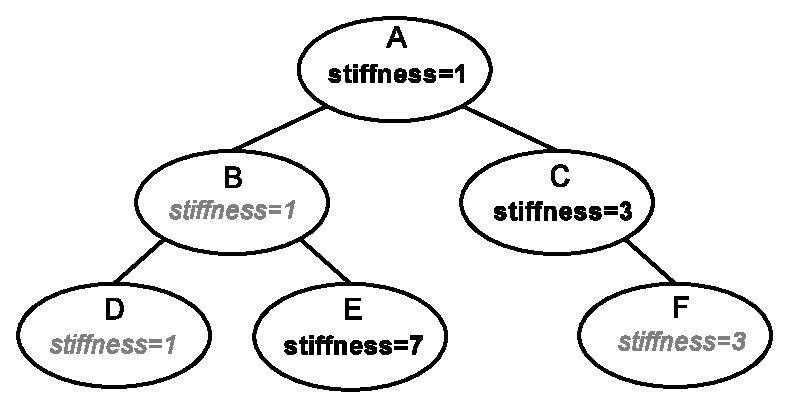
\includegraphics[width=3.75in]{images/inheritedProperties}
\end{center}
\caption{Inheritance of a property named {\it stiffness} among
a component hierarchy. Explicit settings are in bold; inherited settings
are in gray italic.}
\label{inheritedProperties:fig}
\end{figure}

Composite properties are possible, in which a property value is a
composite object that in turn has sub-properties. A good example of
this is the {\tt RenderProps} class, which is
associated with the property {\tt renderProps} for renderable objects
and which itself can have a number of sub-properties such as {\tt
visible}, {\tt faceStyle}, {\tt faceColor}, {\tt lineStyle}, {\tt
lineColor}, etc.

Properties can be declared to be {\tt inheritable}, so that their
values can be inherited from the same properties hosted by ancestor
components further up the component hierarchy. Inheritable properties
require a more elaborate declaration and are associated with a {\it
mode} which may be either {\tt Explicit} or {\tt Inherited}.  If a
property's mode is inherited, then its value is obtained from
the closest ancestor exposing the same property whose mode is
explicit. In Figure (\ref{inheritedProperties:fig}), the property {\it
stiffness} is explicitly set in components A, C, and E, and inherited
in B and D (which inherit from A) and F (which inherits from C).

\section{Creating an application model}
\label{CreatingAnApplication:sec}

ArtiSynth applications are created by writing and compiling
an {\it application model} that is a subclass of {\tt RootModel}.
This application-specific root model is then loaded and run by the
ArtiSynth program.

The code for the application model should:

\begin{itemize}

\item Declare a no-args constructor

\item Override the {\tt RootModel}
\javamethod*[artisynth.core.workspace.RootModel]{build()}
method to construct the application.

\end{itemize}

ArtiSynth can load a model either using the build method
or by reading it from a file:

\begin{description}

\item[Build method] \mbox{}

ArtiSynth creates an instance of the
model using the no-args constructor, assigns it a name
(which is either user-specified or the simple name of the class), and
then calls the {\tt build()} method to perform the actual
construction.

\item[Reading from a file] \mbox{}

ArtiSynth creates an instance of the
model using the no-args constructor, and then the model is named
and constructed by reading the file.

\end{description}

The no-args constructor should perform whatever initialization is
required in both cases, while the {\tt build()} method takes the place of the
file specification. Unless a model is originally created using a file
specification (which is very tedious), the first time
creation of a model will almost always entail using the {\tt build()}
method.

The general template for application model code looks like this:

\begin{lstlisting}[]
package artisynth.models.experimental; // package where the model resides
import artisynth.core.workspace.RootModel;
... other imports ...

public class MyModel extends RootModel {

   // no-args constructor
   public MyModel() {
      ... basic initialization ...
   }

   // build method to do model construction
   public void build (String[] args) {
      ... code to build the model ....
   }
}
\end{lstlisting}
Here, the model itself is called {\tt MyModel}, and is defined in the
(hypothetical) 
package {\tt artisynth.models.experimental} (placing models in the super
package {\tt artisynth.models} is common practice but not
necessary).

\begin{sideblock}
Note: The {\tt build()} method was only introduced in ArtiSynth
3.1. Prior to that, application models were constructed using a
constructor taking a {\tt String} argument supplying the name of the
model. This method of model construction still works but is
deprecated.
\end{sideblock}

\subsection{Implementing the build() method}

As mentioned above, the {\tt build()} method is responsible for actual
model construction.  Many applications are built using a single
top-level {\tt MechModel}.  Build methods for these may look
like the following:
\begin{lstlisting}[]
   public void build (String[] args) {
      MechModel mech = new MechModel("mech");
      addModel (mech);

      ... create and add components to the mech model ...
      ... create and add any needed agents to the root model ...

   }
\end{lstlisting}
First, a \javaclass[artisynth.core.mechmodels]{MechModel} is created
(with the name {\tt "mech"} in this example, although any name, or no
name, may be given) and added to the list of models in the root
model. Subsequent code then creates and adds the components required
by the {\tt MechModel}, as described in Sections
\ref{MechModelsI:sec}, \ref{MechModelsII:sec} and \ref{FEMModels:sec}.
The {\tt build()} method also creates and adds to the root model any
agents required by the application (controllers, probes, etc.), as
described in Section \ref{SimulationControl:sec}.

When constructing a model, there is no fixed order in which components
need to be added. For instance, in the above example, {\tt
addModel(mech)} could be called near the end of the {\tt build()}
method rather than at the beginning. The only restriction is that when
a component is added to the hierarchy, all other components that it
refers to should already have been added to the hierarchy. For
instance, an axial spring (Section \ref{ParticlesAndSprings:sec})
refers to two points. When it is added to the hierarchy, those two
points should already be present in the hierarchy.

The {\tt build()} method supplies a {\tt String} array as an argument,
which can be used to transmit application arguments in a manner
analogous to the {\tt args} argument passed to static {\tt main()}
methods. In cases where the model is specified directly on the
ArtiSynth command line (using the {\tt -model <classname>} option), it
is possible to also specify arguments for the {\tt build()} method.
This is done by enclosing the desired
arguments within square brackets {\tt [ ]} immediately following the
{\tt -model} option. So, for example,
%
\begin{verbatim}
> artisynth -model projects.MyModel [ -foo 123 ]
\end{verbatim}
%
would cause the strings {\tt "-foo"} and {\tt "123"} to
be passed to the {\tt build()} method of {\tt MyModel}.

\subsection{Making models visible to ArtiSynth}

In order to load an application model into ArtiSynth, the classes
associated with its implementation must be made visible to ArtiSynth.
This usually involves adding the top-level class directory associated
with the application code to the classpath used by ArtiSynth.

\begin{sideblock}
The demonstration models referred to in this guide belong to the
package {\tt artisynth.demos.tutorial} and are already visible to
ArtiSynth.
\end{sideblock}

In most current ArtiSynth projects, classes are stored in
a directory tree separate from the source code, with the top-level
class directory named {\tt classes}, located one level below
the project root directory. A typical top-level class directory
might be stored in a location like this:
\begin{verbatim}
  /home/joeuser/artisynthProjects/classes
\end{verbatim}
In the example shown in Section \ref{CreatingAnApplication:sec}, the
model was created in the package {\tt artisynth.models.experimental}.
Since Java classes are arranged in a directory structure that mirrors
package names, with respect to the sample project directory shown
above, the model class would be located in
\begin{verbatim}
  /home/joeuser/artisynthProjects/classes/artisynth/models/experimental
\end{verbatim}

At present there are three ways to make top-level class directories
known to ArtiSynth:

\begin{description}

\item[Add projects to your Eclipse launch configuration]\mbox{}

If you are using the Eclipse IDE, then you can add the project in
which are developing your model code to the launch configuration that
you use to run ArtiSynth. Other IDEs will presumably provide similar
functionality.

\item[Add the directories to the EXTCLASSPATH file]\mbox{}

You can explicitly list class directories in the file EXTCLASSPATH,
located in the ArtiSynth root directory (it may be necessary to create
this file).

\item[Add the directories to your CLASSPATH environment variable]\mbox{}

If you are running ArtiSynth from the command line, using the {\tt
artisynth} command (or {\tt artisynth.bat} on Windows), then you can
define a CLASSPATH environment variable in your environment and add
the needed directories to this.

\end{description}

All of these methods are described in more detail in the ``Installing
External Models and Packages'' section of the ArtiSynth Installation
Guide (available for 
\artisynthManual[installation/linuxInstallation]{linuxInstallation}{Linux}, 
\artisynthManual[installation/windowsInstallation]{windowsInstallation}{Windows},
and 
\artisynthManual[installation/macosInstallation]{macosInstallation}{MacOS}).

\subsection{Loading and running a model}
\label{LoadingAndRunning:sec}

If a model's classes are visible to ArtiSynth, then it may be loaded
into ArtiSynth in several ways:

\begin{description}

\item[Loading by class path]\mbox{}

A model may be loaded by directly by choosing {\sf File > Load from
class ...} and directly specifying its class name. It is also possible
to use the {\tt -model <classname>} command line argument to have a
model loaded directly into ArtiSynth when it starts up.

\item[Loading from the Models menu]\mbox{}

A faster way to load a model is by selecting it in one of the {\sf
Models} submenus. This may require editing the model menu
configuration files.

\item[Loading from a file]\mbox{}

If a model has previously been saved to a file, it may be loaded from
that file by choosing {\sf File > Load model ...}.

\end{description}

These methods are described in detail in the 
section ``Loading and Simulating Models'' of the\pdfbreak
\artisynthManual{uiguide}{ArtiSynth User Interface Guide}.

\begin{sideblock}
The demonstration models referred to in this guide should already
be present in the models menu and may be loaded
from the submenu {\sf Models > All demos > tutorial}.
\end{sideblock}

Once a model is loaded, it can be simulated, or {\it run}.
Simulation
of the model can then be started, paused, single-stepped, or reset
using the play controls (Figure \ref{PlayControlsFig})
located at the upper right of the ArtiSynth window frame.

\begin{figure}[ht]
\begin{center}
\iflatexml
\includegraphics[]{../uiguide/images/playControls}
\else
\includegraphics[width=2.5in]{../uiguide/images/playControls}
\fi
\end{center}
\caption{The ArtiSynth play controls. From left to right: step size
control, current simulation time, and the reset, skip-back,
play/pause, single-step and skip-forward buttons.}%
\label{PlayControlsFig}
\end{figure}

Comprehensive information on exploring and interacting with models is
given in the
\artisynthManual{uiguide}{ArtiSynth User Interface Guide}.

\ifdefined\maindoc
\else
\end{document}
\fi

\section{Supporting classes}

ArtiSynth uses a large number of supporting classes, mostly defined in
the super package {\tt maspack}, for handling mathematical and
geometric quantities. Those that are refered to in this manual are
summarized in this section.

\subsection{Vectors and matrices}

Among the most basic classes are those used to implement vectors and
matrices, defined in {\tt mapack.matrix}. All vector classes implement
the interface \javaclass[maspack.matrix]{Vector} and all matrix
classes implement \javaclass[maspack.matrix]{Matrix}, which provide a
number of standard methods for setting and accessing values and
reading and writing from I/O streams. 

General sized vectors and matrices are implemented by
\javaclass[maspack.matrix]{VectorNd} and
\javaclass[maspack.matrix]{MatrixNd}. These provide all the usual
methods for linear algebra operations such as addition, scaling, and
multiplication:
%
\begin{lstlisting}[]
  VectorNd v1 = new VectorNd (5);        // create a 5 element vector
  VectorNd v2 = new VectorNd (5); 
  VectorNd vr = new VectorNd (5); 
  MatrixNd M = new MatrixNd (5, 5);      // create a 5 x 5 matrix

  M.setIdentity();                       // M = I
  M.scale (4);                           // M = 4*M

  v1.set (new double[] {1, 2, 3, 4, 5}); // set values
  v2.set (new double[] {0, 1, 0, 2, 0});
  v1.add (v2);                           // v1 += v2
  M.mul (vr, v1);                        // vr = M*v1

  System.out.println ("result=" + vr.toString ("%8.3f"));
\end{lstlisting}
%
As illustrated in the above example, vectors and matrices both provide
a {\tt toString()} method that allows their elements to be formated
using a C-printf style format string. This is useful for providing
concise and uniformly formatted output, particularly for diagnostics.
The output from the above example is
%
\begin{verbatim}
  result=   4.000   12.000   12.000   24.000   20.000
\end{verbatim}
%
Detailed specifications for the format string are provided in the
documentation for \javamethod[maspack.util]{NumberFormat.set(String)}.
If either no format string, or the string {\tt "\%g"}, is specified,
{\tt toString()} formats all numbers using the full-precision output
provided by {\tt Double.toString(value)}.

For computational efficiency, a number of fixed-size vectors and
matrices are also provided. The most commonly used are those defined
for three dimensions, including \javaclass[maspack.matrix]{Vector3d}
and \javaclass[maspack.matrix]{Matrix3d}:
%
\begin{lstlisting}[]
  Vector3d v1 = new Vector3d (1, 2, 3);
  Vector3d v2 = new Vector3d (3, 4, 5);
  Vector3d vr = new Vector3d ();
  Matrix3d M = new Matrix3d();

  M.set (1, 2, 3,  4, 5, 6,  7, 8, 9);

  M.mul (vr, v1);        // vr = M * v1
  vr.scaledAdd (2, v2);  // vr += 2*v2;
  vr.normalize();        // normalize vr
  System.out.println ("result=" + vr.toString ("%8.3f"));
\end{lstlisting}
%

\subsection{Rotations and transformations}
\label{RigidTransform3d:sec}

{\tt maspack.matrix} contains a number classes that implement rotation
matrices, rigid transforms, and affine transforms. 

Rotations (Section \ref{Rotations:sec}) are commonly described using a
\javaclass[maspack.matrix]{RotationMatrix3d}, which implements a
rotation matrix and contains numerous methods for setting rotation
values and transforming other quantities. Some of the more commonly
used methods are:
%
\begin{lstlisting}[]
   RotationMatrix3d();         // create and set to the identity
   RotationMatrix3d(u, angle); // create and set using an axis-angle

   setAxisAngle (u, ang);      // set using an axis-angle
   setRpy (roll, pitch, yaw);  // set using roll-pitch-yaw angles
   setEuler (phi, theta, psi); // set using Euler angles
   invert ();                  // invert this rotation
   mul (R)                     // post multiply this rotation by R
   mul (R1, R2);               // set this rotation to R1*R2
   mul (vr, v1);               // vr = R*v1, where R is this rotation
\end{lstlisting}
%
Rotations can also be described by
\javaclass[maspack.matrix]{AxisAngle}, which characterizes a rotation
as a single rotation about a specific axis.

Rigid transforms (Section \ref{RigidTransforms:sec}) are used by
ArtiSynth to describe a rigid body's pose, as well as its relative
position and orientation with respect to other bodies and coordinate
frames.  They are implemented by
\javaclass[maspack.matrix]{RigidTransform3d}, which exposes its
rotational and translational components directly through the fields
{\tt R} (a {\tt RotationMatrix3d}) and {\tt p} (a {\tt
Vector3d}). Rotational and translational values can be set and
accessed directly through these fields.  In addition, {\tt
RigidTransform3d} provides numerous methods, some of the more commonly
used of which include:
%
\begin{lstlisting}[]
   RigidTransform3d();         // create and set to the identity
   RigidTransfrom3d(x, y, z);  // create and set translation to x, y, z

   // create and set translation to x, y, z and rotation to roll-pitch-yaw
   RigidTransfrom3d(x, y, z, roll, pitch, yaw);

   invert ();                  // invert this transform
   mul (T)                     // post multiply this transform by T
   mul (T1, T2);               // set this transform to T1*T2
   mulLeftInverse (T1, T2);    // set this transform to inv(T1)*T2
\end{lstlisting}
%

Affine transforms (Section \ref{AffineTransforms:sec}) are used by
ArtiSynth to effect scaling and shearing transformations on
components. They are implemented by
\javaclass[maspack.matrix]{AffineTransform3d}.

Rigid transformations are actually a specialized form of affine
transformation in which the basic transform matrix equals a rotation.
{\tt RigidTransform3d} and {\tt AffineTransform3d} hence both derive
from the same base class
\javaclass[maspack.matrix]{AffineTransform3dBase}.

\subsection{Points and Vectors}

The rotations and transforms described above can be used to transform
both vectors and points in space.

Vectors are most commonly implemented using
\javaclass[maspack.matrix]{Vector3d}, while points can be implemented
using the subclass \javaclass[maspack.matrix]{Point3d}.  The only
difference between {\tt Vector3d} and {\tt Point3d} is that the former
ignores the translational component of rigid and affine transforms;
i.e., as described in Sections \ref{RigidTransforms:sec} and
\ref{AffineTransforms:sec}, a vector {\tt v} has
an implied homogeneous representation of
%
\begin{equation}
\v^* \equiv \matl \v \\ 0 \matr,
\end{equation}
%
while the representation for a point {\tt p} is
%
\begin{equation}
\p^* \equiv \matl \p \\ 1 \matr.
\end{equation}
%

Both classes provide a number of methods for applying rotational and
affine transforms. Those used for rotations are
%
\begin{lstlisting}[]
  void transform (R);             // this = R * this
  void transform (R, v1);         // this = R * v1
  void inverseTransform (R);      // this = inverse(R) * this
  void inverseTransform (R, v1);  // this = inverse(R) * v1
\end{lstlisting}
%
where {\tt R} is a rotation matrix and {\tt v1} is a vector (or a point
in the case of {\tt Point3d}).

The methods for applying rigid or affine transforms include:
\begin{lstlisting}[]
  void transform (X);             // transforms this by X         
  void transform (X, v1);         // sets this to v1 transformed by X
  void inverseTransform (X);      // transforms this by the inverse of X
  void inverseTransform (X, v1);  // sets this to v1 transformed by inverse of X
\end{lstlisting}
where {\tt X} is a rigid or affine transform.
As described above, in the case of {\tt Vector3d}, these methods
ignore the translational part of the transform and apply only the
matrix component ({\tt R} for a {\tt RigidTransform3d} and {\tt A} for
an {\tt AffineTransform3d}).
In particular, that means that for a {\tt RigidTransform3d} given by {\tt X}
and a {\tt Vector3d} given by {\tt v},
the method calls
%
\begin{lstlisting}[]
  v.transform (X.R)
  v.transform (X)
\end{lstlisting}
%
produce the same result.

\subsection{Spatial vectors and inertias}
\label{SpatialVectors:sec}

The velocities, forces and inertias associated with 3D coordinate
frames and rigid bodies are represented using the 6 DOF spatial
quantities described in Sections \ref{SpatialVelocitiesAndForces:sec}
and \ref{SpatialInertia:sec}. These are implemented by classes in the
package {\tt maspack.spatialmotion}.

Spatial velocities (or twists) are implemented by
\javaclass[maspack.spatialmotion]{Twist}, which exposes its
translational and angular velocity components through the publicly
accessible fields {\tt v} and {\tt w}, while spatial forces (or
wrenches) are implemented by
\javaclass[maspack.spatialmotion]{Wrench}, which exposes its
translational force and moment components through the publicly
accessible fields {\tt f} and {\tt m}.

Both {\tt Twist} and {\tt Wrench} contain methods for algebraic
operations such as addition and scaling. They also contain {\tt
transform()} methods for applying rotational and rigid transforms.
The rotation methods simply transform each component by the supplied
rotation matrix. The rigid transform methods, on the other hand,
assume that the supplied argument represents a transform between two
frames fixed within a rigid body, and transform the twist or wrench
accordingly, using either (\ref{XvelAB:eqn}) or (\ref{XforceAB:eqn}).

The spatial inertia for a rigid body is implemented by
\javaclass[maspack.spatialmotion]{SpatialInertia}, which contains a
number of methods for setting its value given various mass, center of
mass, and inertia values, and querying the values of its components.
It also contains methods for scaling and adding, transforming between
coordinate systems, inversion, and multiplying by spatial vectors.

\subsection{Meshes}
\label{Meshes:sec}

ArtiSynth makes extensive use of 3D meshes, which are defined in {\tt
maspack.geometry}.  They are used for a variety of purposes, including
visualization, collision detection, and computing physical properties
(such as inertia or stiffness variation within a finite element
model).

A mesh is essentially a collection of vertices
(i.e., points) that are topologically connected in some way.  All
meshes extend the abstract base class
\javaclass[maspack.geometry]{MeshBase}, which supports the vertex
definitions, while subclasses provide the topology.

Through {\tt MeshBase}, all meshes provide methods for
adding and accessing vertices. Some of these include:
%
\begin{lstlisting}[]
  int getNumVertices();              // return the number of vertices
  Vertex3d getVertex (int idx);      // return the idx-th vertex
  void addVertex (Vertex3d vtx);     // add vertex vtx to the mesh
  Vertex3d addVertex (Point3d p);    // create and return a vertex at position p
  void removeVertex (Vertex3d vtx);  // remove vertex vtx for the mesh
  ArrayList<Vertex3d> getVertices(); // return the list of vertices
\end{lstlisting}
%
Vertices are implemented by \javaclass[maspack.geometry]{Vertex3d},
which defines the position of the vertex (returned by the method
\javamethod*[maspack.geometry.Vertex3d]{getPosition()}), and also
contains support for topological connections. In addition, each vertex
maintains an index, obtainable via
\javamethod*[maspack.geometry.Vertex3d]{getIndex()}, that equals the
index of its location within the mesh's vertex list. This makes it
easy to set up parallel array structures for augmenting mesh vertex
properties.

Mesh subclasses currently include:

\begin{description}

\item[\protect{\javaclass[maspack.geometry]{PolygonalMesh}}]\mbox{}

Implements a 2D surface
mesh containing faces implemented using half-edges.

\item[\protect{\javaclass[maspack.geometry]{PolylineMesh}}]\mbox{}

Implements a mesh
consisting of connected line-segments (polylines).

\item[\protect{\javaclass[maspack.geometry]{PointMesh}}]\mbox{}

Implements a point cloud with
no topological connectivity.

\end{description}

\javaclass[maspack.geometry]{PolygonalMesh} is used quite extensively
and provides a number of methods for implementing faces, including:
%
\begin{lstlisting}[]
  int getNumFaces();              // return the number of faces
  Face getFace (int idx);         // return the idx-th face
  Face addFace (int[] vidxs);     // create and add a face from specified vertex indices
  void removeFace (Face f);       // remove the face f
  ArrayList<Face> getFaces();     // return the list of faces
\end{lstlisting}
%
The class \javaclass[maspack.geometry]{Face} implements a face as a
counter-clockwise arrangement of vertices linked together by
half-edges (class \javaclass[maspack.geometry]{HalfEdge}).
{\tt Face} also supplies a face's (outward facing) normal
via 
\javamethod[maspack.geometry.Face]{getNormal()}.

Some mesh uses within ArtiSynth, such as collision detection, require a
{\it triangular} mesh; i.e., one where all faces have three vertices.
The method \javamethod[maspack.geometry.PolygonalMesh]{isTriangular()}
can be used to check for this. Meshes that are not triangular can be
made triangular using 
\javamethod[maspack.geometry.PolygonalMesh]{triangulate()}.

\subsubsection{Mesh creation}

It is possible to create a mesh by direct construction. For example,
the following code fragment creates a simple closed tetrahedral
surface:
%
\begin{lstlisting}[]
   // a simple four-faced tetrahedral mesh 
   PolygonalMesh mesh = new PolygonalMesh();
   mesh.addVertex (0, 0, 0);
   mesh.addVertex (1, 0, 0);
   mesh.addVertex (0, 1, 0);
   mesh.addVertex (0, 0, 1);
   mesh.addFace (new int[] { 0, 2, 1 });
   mesh.addFace (new int[] { 0, 3, 2 });
   mesh.addFace (new int[] { 0, 1, 3 });
   mesh.addFace (new int[] { 1, 2, 3 });      
\end{lstlisting}
%

However, meshes are more commonly created using either one of the
factory methods supplied by \javaclass[maspack.geometry]{MeshFactory},
or by reading a definition from a file (Section \ref{MeshFileIO:sec}).

Some of the more commonly used factory methods for creating polyhedral
meshes include:
%
\begin{lstlisting}[]
  MeshFactory.createSphere (radius, nslices, nlevels);
  MeshFactory.createBox (widthx, widthy, widthz);
  MeshFactory.createCylinder (radius, height, nslices);
  MeshFactory.createPrism (double[] xycoords, height);
  MeshFactory.createTorus (rmajor, rminor, nmajor, nminor);
\end{lstlisting}
%
Each factory method creates a mesh in some standard coordinate
frame. After creation, the mesh can be transformed using the
\javamethodAlt{maspack.geometry.MeshBase.transform(AffineTransform3dBase)}%
{transform(X)} method, where {\tt X} is either a rigid transform (
\javaclass[maspack.matrix]{RigidTransform3d}) or a more general affine
transform (\javaclass[maspack.matrix]{AffineTransform3d}).
For example, to create a rotated box centered on $(5, 6, 7)$,
one could do:
%
\begin{lstlisting}[]
  // create a box centered at the origin with widths 10, 20, 30:
  PolygonalMesh box = MeshFactor.createBox (10, 20, 20);

  // move the origin to 5, 6, 7 and rotate using roll-pitch-yaw
  // angles 0, 0, 45 degrees:
  box.transform (
     new RigidTransform3d (5, 6, 7,  0, 0, Math.toRadians(45)));
\end{lstlisting}
%
One can also scale a mesh using
\javamethodAlt{maspack.geometry.MeshBase.scale(double)}{scale(s)},
where {\tt s} is a single scale factor, or
\javamethodAlt{maspack.geometry.MeshBase.scale(double,double,double)}%
{scale(sx,sy,sz)}, where {\tt sx}, {\tt sy}, and {\tt sz} are separate
scale factors for the x, y and z axes. This provides a useful way to
create an ellipsoid:
%
\begin{lstlisting}[]
   // start with a unit sphere with 12 slices and 6 levels ...
  PolygonalMesh ellipsoid = MeshFactor.createSphere (1.0, 12, 6);

  // and then turn it into an ellipsoid by scaling about the axes:
  ellipsoid.scale (1.0, 2.0, 3.0);
\end{lstlisting}
%
\javaclass[maspack.geometry]{MeshFactory} can also be used to create
new meshes by performing boolean operations on existing ones:
%
\begin{lstlisting}[]
  MeshFactory.getIntersection (mesh1, mesh2);
  MeshFactory.getUnion (mesh1, mesh2);
  MeshFactory.getSubtraction (mesh1, mesh2);
\end{lstlisting}
%

\subsubsection{Reading and writing mesh files}
\label{MeshFileIO:sec}

The package {\tt maspack.geometry.io} supplies a number of classes for
writing and reading meshes to and from files of different formats.

Some of the supported formats and their associated readers and writers
include:

\begin{tabular}{|lll|}
\hline
Extension & Format & Reader/writer classes \\
\hline
.obj & Alias Wavefront & \tt WavefrontReader, WavefrontWriter \\
.ply & Polygon file format & \tt PlyReader, PlyWriter \\
.stl & STereoLithography & \tt StlReader, StlWriter \\
.gts & GNU triangulated surface & \tt GtsReader, GtsWriter \\
.off & Object file format & \tt OffReader, OffWriter \\
\hline
\end{tabular}

The general usage pattern for these classes is to construct the
desired reader or writer with a path to the desired file, and then
call {\tt readMesh()} or {\tt writeMesh()} as appropriate:
%
\begin{lstlisting}[]
   // read a mesh from a .obj file:
   WavefrontReader reader = new WavefrontReader ("meshes/torus.obj");
   PolygonalMesh mesh = null;
   try {
      mesh = reader.readMesh();
   }
   catch (IOException e) {
      System.err.println ("Can't read mesh:");
      e.printStackTrace();
   }
\end{lstlisting}
%
Both {\tt readMesh()} and {\tt writeMesh()} may throw I/O exceptions,
which must be either caught, as in the example above, or
thrown out of the calling routine.

For convenience, one can also use the classes
\javaclass[maspack.geometry.io]{GenericMeshReader} or
\javaclass[maspack.geometry.io]{GenericMeshWriter}, which internally
create an appropriate reader or writer based on the file
extension. This enables the writing of code
that does not depend on the file format:
%
\begin{lstlisting}[]
   String fileName;
   ...
   PolygonalMesh mesh = null;
   try {
      mesh = (PolygonalMesh)GenericMeshReader.readMesh(fileName);
   }
   catch (IOException e) {
      System.err.println ("Can't read mesh:");
      e.printStackTrace();
   }
\end{lstlisting}
%
Here, {\tt fileName} can refer to a mesh of any format supported by
{\tt GenericMeshReader}. Note that the mesh returned by {\tt
readMesh()} is explicitly cast to {\tt PolygonalMesh}.  This is
because {\tt readMesh()} returns the superclass {\tt MeshBase}, since
the default mesh created for some file formats may be different from
{\tt PolygonalMesh}.

\ifdefined\maindoc\else
% typesetting this chapter as a standalone document
\def\doctitle{Mechanical Models I}
% starting definitions for both the main document and stand-alone chapters
\documentclass{book}

\def\mech{artisynth.core.mechmodels}
\def\mgeo{maspack.geometry}

% Add search paths for input files
\makeatletter
\def\input@path{{../}{../../}{../texinputs/}}
\makeatother

\usepackage{amsmath}
\usepackage{framed}
%%
%% Default settings for artisynth
%%
\NeedsTeXFormat{LaTeX2e}
%%\ProvidesPackage{artisynthDoc}[2012/04/05]

\usepackage[T1]{fontenc}
\usepackage[latin1]{inputenc}
\usepackage{listings}
\usepackage{makeidx}
\usepackage{latexml}
\usepackage{graphicx}
\usepackage{framed}
\usepackage{booktabs}
\usepackage{color}

\newcommand{\pubdate}{\today}
\newcommand{\setpubdate}[1]{\renewcommand{\pubdate}{#1}}
\newcommand{\code}[1]{{\tt #1}}

\iflatexml
\usepackage{hyperref}
\setlength\parindent{0pt} 
\else
%% then we are making a PDF, so include things that LaTeXML can't handle: 
%% docbook style, \RaggedRight
\usepackage{ifxetex}
\usepackage{xstring}
\usepackage{pslatex} % fixes fonts; in particular sets a better-fitting \tt font

\usepackage[most]{tcolorbox}
\definecolor{shadecolor}{rgb}{0.95,0.95,0.95}
\tcbset{
    frame code={}
    center title,
    left=0pt,
    right=0pt,
    top=0pt,
    bottom=0pt,
    colback=shadecolor,
    colframe=white,
    width=\dimexpr\textwidth\relax,
    enlarge left by=0mm,
    boxsep=0pt,
    arc=0pt,outer arc=0pt,
}%

\usepackage[A4]{artisynth_papersize}
%\usepackage[letter]{artisynth_papersize}
\usepackage[hyperlink]{asciidoc-dblatex} 

%\usepackage{verbatim}
\usepackage{ragged2e}
\setlength{\RaggedRightRightskip}{0pt plus 4em}
\RaggedRight
\renewcommand{\DBKpubdate}{\pubdate}
\renewcommand{\DBKreleaseinfo}{}
\fi

% set hypertext links to be dark blue:
\definecolor{darkblue}{rgb}{0,0,0.8}
\definecolor{sidebar}{rgb}{0.5,0.5,0.7}
\hypersetup{colorlinks=true,urlcolor=darkblue,linkcolor=darkblue,breaklinks=true}

%%%%%%%%%%%%%%%%%%%%%%%%%%%%%%%%%%%%%%%%%%%%%%%%%%%%%%%%%%%%%%%%%%%%%%%%%%%%%
%
% Define macros for handling javadoc class and method references
%
%%%%%%%%%%%%%%%%%%%%%%%%%%%%%%%%%%%%%%%%%%%%%%%%%%%%%%%%%%%%%%%%%%%%%%%%%%%%%
\makeatletter

% macro to enable line break if inside a PDF file
\def\pdfbreak{\iflatexml\else\\\fi}

% code inspired by http://stackoverflow.com/questions/2457780/latex-apply-an-operation-to-every-character-in-a-string
\def\removeargs #1{\doremoveargs#1$\wholeString\unskip}
\def\doremoveargs#1#2\wholeString{\if#1$%
\else\if#1({()}\else{#1}\taketherest#2\fi\fi}
\def\taketherest#1\fi
{\fi \doremoveargs#1\wholeString}

% Note: still doesn't work properly when called on macro output ...
% i.e., \dottoslash{\concatnames{model}{base}{foo}} fails 
\def\dottoslash #1{\dodottoslash#1$\wholeString\unskip}
\def\dodottoslash#1#2\wholeString{\if#1$%
\else\if#1.{/}\else{#1}\fi\dottaketherest#2\fi}
\def\dottaketherest#1\fi{\fi \dodottoslash#1\wholeString}

\def\hashtodot #1{\dohashtodot#1$\wholeString\unskip}
\def\dohashtodot#1#2\wholeString{\if#1$X%
\else\if#1\#{.}\else{#1}\fi\hashtaketherest#2\fi}
\def\hashtaketherest#1\fi{\fi \dohashtodot#1\wholeString}

%\dollartodot{#1} does the same thing as \StrSubstitute[0]{#1}{\$}{.}
% from the packahe xstring. We define \dollartodot instead because
% LaTeXML does not implement xstring.
%
% Note that for the substituion to work, we need \ifx instead of \if,
% since otherwise escaped characters won't work properly:
% if #1 = \$, then \if#1* seems to compare '\' and '$' (and output '*'),
% rather than comparing '$' to '*'
\def\dollartodot #1{\dodollartodot#1*\wholeString\unskip}
\def\dodollartodot#1#2\wholeString{\ifx#1*%
\else \ifx#1\${.}\else{#1}\fi\dollartaketherest#2\fi}
\def\dollartaketherest#1\fi{\fi \dodollartodot#1\wholeString}

% concatenates up to three class/method names together, adding '.' characters
% between them. The first and/or second argument may be empty, in which case
% the '.' is omitted. To check to see if these arguments are empty, we
% use a contruction '\if#1@@', which will return true iff #1 is empty
% (on the assumption that #1 will not contain a '@' character).
\def\concatnames
#1#2#3{\if#1@@\if#2@@#3\else #2.#3\fi\else\if#2@@#1.#3\else#1.#2.#3\fi\fi}

\newcommand{\javabase}{}
\newcommand{\setjavabase}[1]{\renewcommand{\javabase}{#1}}

\def\artisynthDocBase{@ARTISYNTHDOCBASE}

\iflatexml
\def\ifempty#1{\def\temp{#1}\ifx\temp\empty}%
\newcommand{\artisynthManual}[3][]{%
   \ifempty{#1}
      \href{@ARTISYNTHDOCBASE/#2/#2.html}{#3}%
    \else
      \href{@ARTISYNTHDOCBASE/#1/#2.html}{#3}%
    \fi
}
\else
\newcommand{\artisynthManual}[3][]{%
\href{https://www.artisynth.org/@ARTISYNTHDOCBASE/#2.pdf}{#3}}
\fi

%\href{@ARTISYNTHDOCBASE/#2/#2.html}{#3}}



\newcommand{\javaclassx}[2][]{%
% Includes code to prevent an extra '.' at the front if #1 is empty. It
% works like this: if '#1' is empty, then '#1.' expands to '.', and so 
% '\if#1..' will return true, in which case we just output '#2'.
\href{@JDOCBEGIN/\concatnames{\javabase}{#1}{#2}@JDOCEND}{#2}}
\newcommand{\javaclass}[2][]{%
\href{@JDOCBEGIN/\concatnames{}{#1}{#2}@JDOCEND}{\dollartodot{#2}}}
\newcommand{\javaclassAlt}[2]{%
\href{@JDOCBEGIN/\concatnames{}{}{#1}@JDOCEND}{#2}}

\newcommand{\javamethodArgsx}[2][]{%
\href{@JDOCBEGIN/\concatnames{\javabase}{#1}{#2}@JDOCEND}{#2}}
\newcommand{\javamethodArgs}[2][]{%
\href{@JDOCBEGIN/\concatnames{}{#1}{#2}@JDOCEND}{#2}}
\newcommand{\javamethodAlt}[2]{%
\href{@JDOCBEGIN/\concatnames{}{}{#1}@JDOCEND}{#2}}
\newcommand{\javamethodAltx}[2]{%
\href{@JDOCBEGIN/\concatnames{\javabase}{}{#1}@JDOCEND}{#2}}

\newcommand{\javamethodNoArgsx}[2][]{%
\href{@JDOCBEGIN/\concatnames{\javabase}{#1}{#2}@JDOCEND}{\removeargs{#2}}}
\newcommand{\javamethodNoArgs}[2][]{%
\href{@JDOCBEGIN/\concatnames{}{#1}{#2}@JDOCEND}{\removeargs{#2}}}

\newcommand{\javamethod}{\@ifstar\javamethodNoArgs\javamethodArgs}
\newcommand{\javamethodx}{\@ifstar\javamethodNoArgsx\javamethodArgsx}

%%%%%%%%%%%%%%%%%%%%%%%%%%%%%%%%%%%%%%%%%%%%%%%%%%%%%%%%%%%%%%%%%%%%%%%%%%%%%
%
% Define macros for sidebars
%
%%%%%%%%%%%%%%%%%%%%%%%%%%%%%%%%%%%%%%%%%%%%%%%%%%%%%%%%%%%%%%%%%%%%%%%%%%%%%

\iflatexml
\newenvironment{sideblock}{\begin{quote}}{\end{quote}}
\else
\usepackage[strict]{changepage}
\definecolor{sidebarshade}{rgb}{1.0,0.97,0.8}
\newenvironment{sideblock}{%
    \def\FrameCommand{%
    \hspace{1pt}%
    {\color{sidebar}\vrule width 2pt}%
    %{\vrule width 2pt}%
    {\color{sidebarshade}\vrule width 4pt}%
    \colorbox{sidebarshade}%
  }%
  \MakeFramed{\advance\hsize-\width\FrameRestore}%
  \noindent\hspace{-4.55pt}% disable indenting first paragraph
  \begin{adjustwidth}{}{7pt}%
  %\vspace{2pt}\vspace{2pt}%
}
{%
  \vspace{2pt}\end{adjustwidth}\endMakeFramed%
}
\fi

\iflatexml
\newenvironment{shadedregion}{%
  \definecolor{shadecolor}{rgb}{0.96,0.96,0.98}%
  \begin{shaded*}%
% Put text inside a quote to create a surrounding blockquote that
% will properly accept the color and padding attributes
  \begin{quote}%
}
{%
  \end{quote}%
  \end{shaded*}%
}
\else
\newenvironment{shadedregion}{%
  \definecolor{shadecolor}{rgb}{0.96,0.96,0.98}%
  \begin{shaded*}%
}
{%
  \end{shaded*}%
}
\fi

% Wanted to create a 'listing' environment because lstlisting is
% tedious to type and because under latexml it may need
% some massaging to get it to work properly. But hard to do
% because of the verbatim nature of listing
%\iflatexml
%\newenvironment{listing}{\begin{lstlisting}}{\end{lstlisting}}%
%\else
%\newenvironment{listing}{\begin{lstlisting}}{\end{lstlisting}}%
%\fi

\iflatexml\else
% fancyhdr was complaining that it wanted a 36pt header height ...
\setlength{\headheight}{36pt}
\fi

% macro for backslash character
\newcommand\BKS{\textbackslash}

% macro for double hyphen (to prevent conversion of -- into -)
\newcommand\DHY{-{}-}

% Convenience stuff
\newcommand{\ifLaTeXMLelse}[2]{%
  \iflatexml %
  #1 %
  \else %
  #2 %
  \fi %
}

\newcommand{\ifLaTeXML}[1]{ %
  \iflatexml %
  #1 %
  \fi %
}

% new methodtable environment for documenting methods

% base width of the method table
\newlength{\methodtablewidth}
\iflatexml
\setlength{\methodtablewidth}{1.6\textwidth}
\else
\setlength{\methodtablewidth}{0.94\textwidth}
\fi
% horizontal space added at end of call to \methodentry
\newlength{\methodskip}
\setlength{\methodskip}{0pt}
% lengths set inside methodtable environment:
\newlength{\methodsiglength} % length of the method signature
\newlength{\methodcomlength} % length of the method comment
\setlength{\methodsiglength}{0.5\methodtablewidth}
\setlength{\methodcomlength}{0.5\methodtablewidth}

% command to add a method to a method table:
% arg #1: package and signature for finding URL
% arg #2: anchor text
% arg #3: comment describing the method
\newcommand{\methodentry}[3]{%
\javamethodAlt{#1}{\parbox[t]{\methodsiglength}{#2}}&
{\parbox[t]{\methodcomlength}{#3}}\\%
\noalign{\vspace{\methodskip}}}

% methodtable environment takes two arguments, both scale factors for
% methodtablewidth:
% arg #1: width of the method signature column
% arg #2: width of the method comment column
\newenvironment{methodtable}[3][0pt]{%
\begingroup
\setlength{\topskip}{0pt}
\setlength{\methodskip}{#1}
\setlength{\methodsiglength}{#2\methodtablewidth}%
\setlength{\methodcomlength}{#3\methodtablewidth}%
\iflatexml
\begin{snugshade}
\else
\begin{tcolorbox}
\fi
\renewcommand{\arraystretch}{1}
\begin{tabular}{ll}}{%
\end{tabular}
\renewcommand{\arraystretch}{1}
\iflatexml
\end{snugshade}
\else
\end{tcolorbox}
\fi
\endgroup}

% commands for added top, mid and bottom lines in the table.
% uses booktabs for PDF, regular hline for HTML
\newcommand{\topline}{\iflatexml\hline\else\toprule\fi}
\newcommand{\midline}{\iflatexml\hline\else\midrule\fi}
\newcommand{\botline}{\iflatexml\hline\else\bottomrule\fi}
\newcommand{\blankline}{%
\multicolumn{2}{l}{\iflatexml{@SPACE}\else\phantom{M}\fi}\\}%
% add vertical space within a two colum method environment
\newcommand{\methodspace}[1]{%
\iflatexml
\multicolumn{2}{l}{@VERTSPACE[#1]}\\
\else
\noalign{\vspace{#1}}%
\fi}%
% break a line and add an indentation of 1em
\newcommand{\brh}{\\\phantom{M}}

\makeatother

\def\matl{\left(\begin{matrix}}
\def\matr{\end{matrix}\right)}

\def\Bthe{\boldsymbol\theta}
\def\Btau{\boldsymbol\tau}
\def\Bom{\boldsymbol\omega}
\def\Bdel{\boldsymbol\delta}
\def\Blam{\boldsymbol\lambda}
\def\Bphi{\boldsymbol\phi}
\def\Bxi{\boldsymbol\xi}
\def\Bgam{\boldsymbol\gamma}
\def\Bsig{\boldsymbol\sigma}
\def\Bnu{\boldsymbol\nu}
\def\Bmu{\boldsymbol\mu}

\def\A{{\bf A}}
\def\B{{\bf B}}
\def\C{{\bf C}}
\def\D{{\bf D}}
\def\F{{\bf F}}
\def\G{{\bf G}}
\def\H{{\bf H}}
\def\I{{\bf I}}
\def\J{{\bf J}}
\def\K{{\bf K}}
\def\Jc{{\bf J}_c}
\def\L{{\bf L}}
\def\M{{\bf M}}
\def\N{{\bf N}}
\def\O{{\bf O}}
\def\P{{\bf P}}
\def\Q{{\bf Q}}
\def\R{{\bf R}}
\def\T{{\bf T}}
\def\U{{\bf U}}
\def\W{{\bf W}}
\def\X{{\bf X}}
\def\Minv{{\bf M}^{-1}}

\def\a{{\bf a}}
\def\b{{\bf b}}
\def\c{{\bf c}}
\def\d{{\bf d}}
\def\e{{\bf e}}
\def\f{{\bf f}}
\def\g{{\bf g}}
\def\k{{\bf k}}
\def\l{{\bf l}}
\def\m{{\bf m}}
\def\n{{\bf n}}
\def\p{{\bf p}}
\def\q{{\bf q}}
\def\r{{\bf r}}
\def\u{{\bf u}}
\def\v{{\bf v}}
\def\w{{\bf w}}
\def\x{{\bf x}}
\def\y{{\bf y}}
\def\z{{\bf z}}

\def\ma{{\bf m}_\alpha}
\def\mb{{\bf m}_\beta}
\def\va{{\bf v}_\alpha}
\def\vb{{\bf v}_\beta}
\def\vp{{\bf v}_\rho}
\def\vk{{\bf v}_k}
\def\ua{{\bf u}_\alpha}
\def\ub{{\bf u}_\beta}
\def\uk{{\bf u}_k}
\def\uj{{\bf u}_j}
\def\mar{{\bf m}_{\alpha r}}
\def\mbr{{\bf m}_{\beta r}}

\def\Maa{{\bf M}_{\alpha\alpha}}
\def\Mab{{\bf M}_{\alpha\beta}}
\def\Mba{{\bf M}_{\beta\alpha}}
\def\Mbb{{\bf M}_{\beta\beta}}
\def\hatMaa{\hat{\bf M}_{\alpha\alpha}}
\def\hatMab{\hat{\bf M}_{\alpha\beta}}
\def\hatMba{\hat{\bf M}_{\beta\alpha}}
\def\hatMbb{\hat{\bf M}_{\beta\beta}}
\def\Mbp{{\bf M}_{\beta\rho}}
\def\Map{{\bf M}_{\alpha\rho}}
\def\Mpa{{\bf M}_{\rho\alpha}}
\def\Mpb{{\bf M}_{\rho\beta}}
\def\Mpp{{\bf M}_{\rho\rho}}
\def\Mbk{{\bf M}_{\beta k}}
\def\Mak{{\bf M}_{\alpha k}}
\def\Mka{{\bf M}_{k\alpha}}
\def\Mkb{{\bf M}_{k\beta}}
\def\Mkk{{\bf M}_{kk}}

\def\Ga{{\bf G}_{\alpha}}
\def\Gp{{\bf G}_{\rho}}
\def\Gaa{{\bf G}_{\alpha\alpha}}
\def\Gab{{\bf G}_{\alpha\beta}}
\def\Gba{{\bf G}_{\beta\alpha}}
\def\Gbb{{\bf G}_{\beta\beta}}
\def\Gap{{\bf G}_{\alpha\rho}}
\def\Gpa{{\bf G}_{\rho\alpha}}
\def\Gbp{{\bf G}_{\beta\rho}}
\def\Gak{{\bf G}_{\alpha k}}
\def\Gka{{\bf G}_{k\alpha}}
\def\Gja{{\bf G}_{j\alpha}}
\def\Gkb{{\bf G}_{k\beta}}
\def\Gbk{{\bf G}_{\beta k}}

\def\lama{\Blam_{\alpha}}
\def\lamb{\Blam_{\beta}}
\def\lamp{\Blam_{\rho}}
\def\lamk{\Blam_{k}}
\def\lams{\Blam_{\sigma}}

\def\ba{{\bf b}_{\alpha}}
\def\bb{{\bf b}_{\beta}}
\def\fp{{\bf f}_{\rho}}
\def\fa{{\bf f}_{\alpha}}
\def\qa{{\bf q}_{\alpha}}
\def\qb{{\bf q}_{\beta}}
\def\za{{\bf z}_{\alpha}}
\def\zb{{\bf z}_{\beta}}
\def\wa{{\bf w}_{\alpha}}
\def\wb{{\bf w}_{\beta}}

\def\Na{\bar{\bf N}_{\alpha}}
\def\Nb{\bar{\bf N}_{\beta}}

\def\Up{{\bf U}_p}
\def\Un{{\bf U}_n}

\def\dFdl{\frac{\partial F}{\partial l}}
\def\dFddl{\frac{\partial F}{\partial \dot l}}

\def\Sr{s_\theta}
\def\Cr{c_\theta}
\def\Sp{s_\phi}
\def\Cp{c_\phi}
\def\Sy{s_\psi}
\def\Cy{c_\psi}
\def\Sa{s_{\alpha}}
\def\Ca{c_{\alpha}}
\def\Vp{v_{\phi}}


\iflatexml
\else
\usepackage{biblatex}
\addbibresource{references.bib}
\fi

\setcounter{tocdepth}{5}
\setcounter{secnumdepth}{3}

\title{\doctitle}
\ifdefined\maindoc
\author{John Lloyd and Antonio S\'anchez}
\setpubdate{Last update: March, 2021}

\iflatexml
\date{}
\fi
\fi

% graphics paths
\graphicspath{{./}{images/}}

% Listings settings
\definecolor{myblue}{rgb}{0,0,0.6}
\definecolor{mygreen}{rgb}{0,0.6,0}
\definecolor{mygray}{rgb}{0.5,0.5,0.5}
\definecolor{mylightgray}{rgb}{0.95,0.95,0.95}
\definecolor{mymauve}{rgb}{0.58,0,0.82}
\definecolor{myblack}{rgb}{0,0,0}
\lstset{
   language=Java,                   % text highlighting for Java
   breakatwhitespace=false,         % automatic breaks only at whitespace
   breaklines=true,                 % automatic line breaking
   commentstyle=\color{mygreen},    % comment style
   keepspaces=true,                 % keeps spaces in text
   keywordstyle=\color{myblue},     % keyword style
   numbers=none,                    % line-numbers; values: (none, left, right)
   numbersep=5pt,                   % how far the line-numbers are from code
   numberstyle=\tiny\color{mygray}, % line-numbers style
   showspaces=false,                % show spaces everywhere
   showstringspaces=false,          % underline spaces within strings
   showtabs=false,                  % show tabs
   stepnumber=1,                    % the step between two line-numbers
   stringstyle=\color{mymauve},     % string literal style
   tabsize=3,                       % sets default tabsize to 3 spaces
   backgroundcolor=\color{mylightgray}, % background color
   frame=single, 					% adds a frame around the code
   rulesepcolor=\color{mygray},
   rulecolor=\color{myblack},
   framerule=0pt,
   xleftmargin=2.2ex,               % numbers inside box
   framexleftmargin=2.2ex,			% indentation of frame
}

\begin{document}

\frontmatter

%\layout
\maketitle

\iflatexml{\large\pubdate}\fi

\tableofcontents

\mainmatter
\fi

\chapter{Mechanical Models I}
\label{MechModelsI:sec}

This section details how to build basic multibody-type mechanical
models consisting of particles, springs, rigid bodies, joints, and
other constraints.

\section{Springs and particles}
\label{ParticlesAndSprings:sec}

The most basic type of mechanical model consists simply of particles
connected together by axial springs.  Particles are implemented by the
class \javaclass[artisynth.core.mechmodels]{Particle}, which is a
dynamic component containing a three-dimensional position state, a
corresponding velocity state, and a mass. It is an instance of the
more general base class \javaclass[artisynth.core.mechmodels]{Point},
which is used to also implement spatial points such as {\tt markers}
which do not have a mass.

\subsection{Axial springs and materials}
\label{AxialSprings:sec}

An axial spring is a simple spring that connects two points and is
implemented by the class
\javaclass[artisynth.core.mechmodels]{AxialSpring}. This is a {\it
force effector} component that exerts equal and opposite forces on the
two points, along the line separating them, with a magnitude $f$ that
is a function $f(l, \dot l)$ of the distance $l$ between the points,
and the distance derivative $\dot l$.

Each axial spring is associated with an {\it axial material},
implemented by a subclass of
\javaclass[artisynth.core.materials]{AxialMaterial}, that specifies
the function $f(l, \dot l)$. The most basic type of axial material is
a \javaclass[artisynth.core.materials]{LinearAxialMaterial}, which
determines $f$ according to the linear relationship
%
\begin{equation}
f(l, \dot l) = k (l-l_0) + d \dot l
\end{equation}
%
where $l_0$ is the rest length and $k$ and $d$ are the stiffness and
damping terms. Both $k$ and $d$ are properties of the material, while
$l_0$ is a property of the spring.

Axial springs are assigned a linear axial material by default.  More
complex, nonlinear axial materials may be defined in the package {\tt
artisynth.core.materials}. Setting or querying a spring's material
may be done with the methods {\tt setMaterial()} and {\tt
getMaterial()}.

\subsection{Example: a simple particle-spring model}
\label{ParticleSpringExample:sec}

\begin{figure}[t]
\begin{center}
\iflatexml
 \includegraphics[]{images/ParticleSpring}
\else
 \includegraphics[width=3.75in]{images/ParticleSpring}
\fi
\end{center}
\caption{ParticleSpring model loaded into ArtiSynth.}
\label{ParticleSpring:fig}
\end{figure}

An complete application model that implements a simple particle-spring
model is given below. 
\lstset{numbers=left}
\lstinputlisting{../../src/artisynth/demos/tutorial/ParticleSpring.java}
\lstset{numbers=none}

Line 1 of the source defines the package in which the model class will
reside, in this case {\tt artisynth.demos.tutorial}. Lines 3-8 import
definitions for other classes that will be used.

The model application class is named {\tt ParticleSpring} and declared
to extend {\tt RootModel} (line 13), and the {\tt build()} method
definition begins at line 15. (A no-args constructor is also needed,
but because no other constructors are defined, the compiler creates
one automatically.)

To begin, the {\tt build()} method creates a {\tt MechModel} named
{\tt "mech"}, and then adds it to the {\tt models} list of the root model
using the {\tt addModel()} method (lines 18-19). Next, two particles,
{\tt p1} and {\tt p2}, are created, with masses equal to 2 and initial
positions at 0, 0, 0, and 1, 0, 0, respectively (lines 22-23). Then an
axial spring is created, with end points set to {\tt p1} and {\tt p2},
and assigned a linear material with a stiffness and damping of 20 and
10 (lines 24-27). Finally, after the particles and the spring are
created, they are added to the {\tt particles} and {\tt axialSprings}
lists of the {\tt MechModel} using the methods {\tt
addParticle()} and {\tt addAxialSpring()} (lines 30-32).

At this point in the code, both particles are defined to be
dynamically controlled, so that running the simulation would cause
both to fall under the {\tt MechModel}'s default gravity acceleration
of $(0, 0, -9.8)$. However, for this example, we want the first
particle to remain fixed in place, so we set it to be {\it
non-dynamic} (line 34), meaning that the physical simulation will not
update its position in response to forces (Section
\ref{DynamicVsParametric:sec}).

The remaining calls control aspects of how the model is graphically
rendered.  {\tt setBounds()} (line 37) increases the model's
``bounding box'' so that by default it will occupy a larger part of
the viewer frustum. The convenience method {\tt
RenderProps.setSphericalPoints()} is used to set points {\tt p1} and
{\tt p2} to render as solid red spheres with a radius of 0.06, while
{\tt RenderProps.setCylindricalLines()} is used to set {\tt spring} to
render as a solid blue cylinder with a radius of 0.02. More details
about setting render properties are given in Section
\ref{RenderProperties:sec}.

To run this example in ArtiSynth, select {\sf All demos > tutorial >
ParticleSpring} from the {\sf Models} menu. The model should load and
initially appear as in Figure \ref{ParticleSpring:fig}.  Running
the model (Section \ref{LoadingAndRunning:sec}) will
cause the second particle to fall and swing about under gravity.

\subsection{Dynamic, parametric, and attached components}
\label{DynamicVsParametric:sec}

By default, a dynamic component is advanced through time in response
to the forces applied to it. However, it is also possible to set a
dynamic component's {\tt dynamic} property to {\tt false}, so that it
does not respond to force inputs.  As shown in the example above, this
can be done using the method
{\tt setDynamic()}:
%
\begin{verbatim}
  comp.setDynamic (false);
\end{verbatim}
%
The method
\javamethod*[artisynth.core.mechmodels.DynamicAgent]{isDynamic()}
can be used to query the {\tt dynamic} property.

Dynamic components can also be {\it attached} to other dynamic
components (as mentioned in Section \ref{PhysicsSimulation:sec}) so
that their positions and velocities are controlled by the {\it master}
components that they are attached to.  To attach a dynamic component,
one creates an {\tt AttachmentComponent} specifying the attachment
connection and adds it to the {\tt MechModel}, as described in Section
\ref{Attachments:sec}.  The method
\javamethod*[artisynth.core.mechmodels.DynamicAgent]{isAttached()}
can be used to determine if a component is attached, and if it is,
\javamethod*[artisynth.core.mechmodels.DynamicAgent]{getAttachment()}
can be used to find the corresponding {\tt AttachmentComponent}.

Overall, a dynamic component can be in one of three states:

\begin{description}

\item[active]\mbox{}

Component is dynamic and unattached. The method
\javamethod*[artisynth.core.mechmodels.DynamicAgent]{isActive()}
returns {\tt true}. The component will move in response to forces.

\item[parametric]\mbox{}

Component is not dynamic, and is unattached. 
The method
\javamethod*[artisynth.core.mechmodels.DynamicAgent]{isParametric()}
returns {\tt true}.
The component will either remain
fixed, or will move around in response to external inputs specifying
the component's position and/or velocity. One way to supply such
inputs is to use controllers or input probes, as described in
Section \ref{SimulationControl:sec}.

\item[attached]\mbox{}

Component is attached. The method
\javamethod*[artisynth.core.mechmodels.DynamicAgent]{isAttached()}
returns {\tt true}. The component will move so as to follow the other
master component(s) to which it is attached.

\end{description}

\subsection{Custom axial materials}
\label{CustomAxialMaterials:sec}

Application authors may create their
own axial materials by subclassing 
\javaclass[artisynth.core.materials]{AxialMaterial}
and overriding the functions
% method table
\begin{lstlisting}[]
  double computeF (l, ldot, l0, excitation);
  double computeDFdl (l, ldot, l0, excitation);
  double computeDFdldot (l, ldot, l0, excitation);
  boolean isDFdldotZero ();
\end{lstlisting}
%
where {\tt excitation} is an additional {\it excitation} signal $a$, which
is used to implement active springs and which in particular is used to
implement axial muscles (Section \ref{PointToPointMuscles:sec}), for
which $a$ is usually in the range $[0, 1]$.

The first three methods should return the values of 
%
\begin{equation}
f (l, \dot l, a), \quad
\frac{\partial f(l, \dot l, a)}{\partial l}, \quad \text{and} \quad
\frac{\partial f(l, \dot l, a)}{\partial \dot l},
\end{equation}
%
respectively, while the last method should return {\tt true} if
$\partial f(l, \dot l, a) / \partial \dot l \equiv 0$; i.e., if it is
always equals to 0.

\subsection{Damping parameters}
\label{BodyDamping:sec}

Mechanical models usually contain damping forces in addition to
spring-type restorative forces. Damping generates forces that reduce
dynamic component velocities, and is usually the major source of
energy dissipation in the model. Damping forces can be generated by
the spring components themselves, as described above.

A general damping can be set for all particles by setting the
{\tt MechModel}'s {\tt pointDamping} property. This causes
a force
%
\begin{equation}
\f_i = -d_p \v_i \label{eqn:pointdamping}
\end{equation}
%
to be applied to all particles, where $d_p$ is the value of the {\tt
pointDamping} and $\v_i$ is the particle's velocity.

{\tt pointDamping} can be set and queried using the {\tt MechModel}
methods
% method table
\begin{lstlisting}[]
  setPointDamping (double d);
  double getPointDamping();
\end{lstlisting}
%

\begin{sideblock}
In general, whenever a component has a property {\tt propX}, that
property can be set and queried in code using methods of the form
\begin{verbatim}
  setPropX (T d);
  T getPropX();
\end{verbatim}
where {\tt T} is the type associated with the property.
\end{sideblock}

{\tt pointDamping} can also be set for particles individually.  This
property is {\it inherited} (Section
\ref{CompositeInheritableProperties:sec}), so that if not set
explicitly, it inherits the nearest explicitly set value in an
ancestor component.

\section{Rigid bodies}

Rigid bodies are implemented in ArtiSynth by the class
\javaclass[artisynth.core.mechmodels]{RigidBody}, which is a dynamic
component containing a six-dimensional position and orientation state,
a corresponding velocity state, an inertia, and an optional surface
mesh.

A rigid body is associated with its own 3D spatial coordinate frame,
and is a subclass of the more general
\javaclass[artisynth.core.mechmodels]{Frame} component.
The combined position and orientation of this frame with respect to
world coordinates defines the body's {\it pose}, and the associated 6
degrees of freedom describe its ``position'' state.

\subsection{Frame markers}
\label{FrameMarkers:sec}

\begin{figure}[t]
\begin{center}
 \iflatexml
   \includegraphics[width=2.5in]{images/frameMarker}
 \else
   \includegraphics[width=2.5in]{images/frameMarker}
 \fi
\end{center}
\caption{A force $\f$ applied to a frame marker attached to a rigid
body. The marker is located at the point $\r$ with respect to the body
coordinate frame B.}
\label{frameMarker:fig}
\end{figure}

ArtiSynth makes extensive use of {\it markers}, which are (massless)
points attached to dynamic components in the model. Markers are used
for graphical display, implementing attachments, and transmitting
forces back onto the underlying dynamic components.

A {\it frame marker} is a marker that can be attached to a
\javaclass[artisynth.core.mechmodels]{Frame}, and most commonly to a
\javaclass[artisynth.core.mechmodels]{RigidBody} (Figure
\ref{frameMarker:fig}). They are frequently used to provide the
anchor points for attaching springs and, more generally, applying
forces to the body.

Frame markers are implemented by the class
\javaclass[artisynth.core.mechmodels]{FrameMarker}, which
is a subclass of
\javaclass[artisynth.core.mechmodels]{Point}.
The methods
% method table
\begin{lstlisting}[]
  Point3d getLocation();
  void setLocation (Point3d r);
\end{lstlisting}
%
get and set the marker's location $\r$ with respect to the frame's
coordinate system. When a 3D force $\f$ is applied to the marker, it
generates a spatial force $\hat\f$ (Section
\ref{SpatialVelocitiesAndForces:sec}) on the frame given by
%
\begin{equation}
\hat\f = \matl \f \\ \r \times \f \matr.
\end{equation}
%

Frame markers can be created using a variety of constructors, including
% method table
\begin{lstlisting}[]
  FrameMarker ();
  FrameMarker (String name);
  FrameMarker (Frame frame, Point3d loc);
\end{lstlisting}
%
where {\tt FrameMarker()} creates an empty marker, {\tt
FrameMarker(name)} creates an empty marker with a name, and {\tt
FrameMarker(frame,loc)} creates an unnamed marker attached to {\tt
frame} at the location {\tt loc} with respect to the frame's
coordinates. Once created, a marker's frame can be set and queried
with
% method table
\begin{lstlisting}[]
  void setFrame (Frame frame);
  Frame getFrame (); 
\end{lstlisting}
%
A frame marker can be added to a \javaclass[\mech]{MechModel} with the
{\tt MechModel} methods
% method table
\begin{lstlisting}[]
  void addFrameMarker (FrameMarker mkr);
  void addFrameMarker (FrameMarker mkr, Frame frame, Point3d loc);
\end{lstlisting}
%
where {\tt addFrameMarker(mkr,frame,loc)} also sets the frame and the
marker's location with respect to it. 

{\tt MechModel} also supplies convenience methods to create a
marker, attach it to a frame, and add it to the model:
% method table
\begin{lstlisting}[]
  FrameMarker addFrameMarker (Frame frame, Point3d loc);
  FrameMarker addFrameMarkerWorld (Frame frame, Point3d locw);
\end{lstlisting}
%
Both methods return the created marker. 
The first, {\tt addFrameMarker(frame,loc)}, places it at the
location {\tt loc} with respect to the frame, while {\tt
addFrameMarkerWorld(frame,pos)} places it at {\tt pos} with respect to
{\it world} coordinates.

\subsection{Example: a simple rigid body-spring model}
\label{RigidBodySpringExample:sec}

\begin{figure}[ht]
\begin{center}
\iflatexml
 \includegraphics[]{images/RigidBodySpring}
\else
 \includegraphics[width=3.75in]{images/RigidBodySpring}
\fi
\end{center}
\caption{RigidBodySpring model loaded into ArtiSynth.}
\label{RigidBodySpring:fig}
\end{figure}

A simple rigid body-spring model is defined in
%
\begin{verbatim}
  artisynth.demos.tutorial.RigidBodySpring
\end{verbatim}
%
This differs from ParticleSpring only in the {\tt build()} method,
which is listed below:
\lstset{numbers=left}
\begin{lstlisting}[]
   public void build (String[] args) {

      // create MechModel and add to RootModel
      MechModel mech = new MechModel ("mech");
      addModel (mech);

      // create the components
      Particle p1 = new Particle ("p1", /*mass=*/2, /*x,y,z=*/0, 0, 0);
      // create box and set its pose (position/orientation):
      RigidBody box =
         RigidBody.createBox ("box", /*wx,wy,wz=*/0.5, 0.3, 0.3, /*density=*/20);
      box.setPose (new RigidTransform3d (/*x,y,z=*/0.75, 0, 0));
      // create marker point and connect it to the box:
      FrameMarker mkr = new FrameMarker (/*x,y,z=*/-0.25, 0, 0);
      mkr.setFrame (box);

      AxialSpring spring = new AxialSpring ("spr", /*restLength=*/0);
      spring.setPoints (p1, mkr);
      spring.setMaterial (
         new LinearAxialMaterial (/*stiffness=*/20, /*damping=*/10));

      // add components to the mech model
      mech.addParticle (p1);
      mech.addRigidBody (box);
      mech.addFrameMarker (mkr);
      mech.addAxialSpring (spring);

      p1.setDynamic (false);               // first particle set to be fixed

      // increase model bounding box for the viewer
      mech.setBounds (/*min=*/-1, 0, -1, /*max=*/1, 0, 0);  
      // set render properties for the components
      RenderProps.setSphericalPoints (p1, 0.06, Color.RED);
      RenderProps.setSphericalPoints (mkr, 0.06, Color.RED);
      RenderProps.setCylindricalLines (mkr, 0.02, Color.BLUE);
   }
\end{lstlisting}
\lstset{numbers=none} 
The differences from {\tt ParticleSpring} begin
at line 9. Instead of creating a second particle, a rigid body is
created using the factory method
\javamethod*[artisynth.core.mechmodels]{RigidBody.createBox(,,,,)}, which
takes x, y, z widths and a (uniform) density and creates a box-shaped
rigid body complete with surface mesh and appropriate mass and
inertia. As the box is initially centered at the origin, moving it
elsewhere requires setting the body's pose, which is done using {\tt
setPose()}. The {\tt RigidTransform3d} passed to {\tt setPose()} is
created using a three-argument constructor that generates a
translation-only transform.  Next, starting at line 14, a {\tt
FrameMarker} is created for a location $(-0.25, 0, 0)^T$ relative to the
rigid body, and attached to the body using its {\tt setFrame()}
method.

The remainder of {\tt build()} is the same as for {\tt ParticleSpring},
except that the spring is attached to the frame marker instead of a
second particle.

To run this example in ArtiSynth, select {\sf All demos > tutorial >
RigidBodySpring} from the {\sf Models} menu. The model should load and
initially appear as in Figure \ref{RigidBodySpring:fig}.  Running the
model (Section \ref{LoadingAndRunning:sec}) will cause the rigid body
to fall and swing about under gravity.

\subsection{Creating rigid bodies}

As illustrated above, rigid bodies can be created using factory
methods supplied by \javaclass[artisynth.core.mechmodels]{RigidBody}.
Some of these include:
% method table
\begin{lstlisting}[]
  createBox (name, widthx, widthy, widthz, density);
  createCylinder (name, radius, height, density, nsides);
  createSphere (name, radius, density, nslices);
  createEllipsoid (name, radx, rady, radz, density, nslices);
\end{lstlisting}
%
The bodies do not need to be named; if no name is desired, then {\tt
name} and can be specified as {\tt null}.

In addition, there are also
factory methods for creating a rigid body directly from a mesh:
% method table
\begin{lstlisting}[]
  createFromMesh (name, mesh, density, scale);
  createFromMesh (name, meshFileName, density, scale);
\end{lstlisting}
%
These take either a polygonal mesh (Section \ref{Meshes:sec}), or a
file name from which a mesh is read, and use it as the body's surface
mesh and then compute the mass and inertia properties from the specified
(uniform) density.

\begin{sideblock}
When a body is created directly from a surface mesh, its center of
mass will typically {\it not} be coincident with the origin of its
coordinate frame. Section \ref{RigidBodyCOM:sec} discusses the
implications of this and how to correct it.
\end{sideblock}

Alternatively, one can create a rigid body directly from a
constructor, and then set the mesh and inertia properties explicitly:
%
\begin{lstlisting}[]
  PolygonalMesh femurMesh;
  SpatialInertia inertia;

  ... initialize mesh and inertia appropriately ...

  RigidBody body = new RigidBody ("femur");
  body.setMesh (femurMesh);
  body.setInertia (inertia);
\end{lstlisting}
%

\subsection{Pose and velocity}

A body's pose can be set and
queried using the methods
% method table
\begin{lstlisting}[]
  setPose (RigidTransform3d T);   // sets the pose to T
  getPose (RigidTransform3d T);   // gets the current pose in T
  RigidTransform3d getPose();     // returns the current pose (read-only)
\end{lstlisting}
%
These use a \javaclass[maspack.matrix]{RigidTransform3d} (Section
\ref{RigidTransform3d:sec}) to describe the pose. Body poses are
described in world coordinates and specify the transform from body to
world coordinates. In particular, the pose for a body A specifies
the rigid transform $\T_{AW}$.

Rigid bodies also expose the translational and rotational components of
their pose via the properties {\tt position} and {\tt orientation},
which can be queried and set independently using the methods
% method table
\begin{lstlisting}[]
  setPosition (Point3d p);       // sets the position to p
  getPosition (Point3d p);       // gets the current position in p
  Point3d getPosition();         // returns the current position (read-only)

  setOrientation (AxisAngle a);  // sets the orientation to a
  getOrientation (AxisAngle a);  // gets the current orientation in a
  AxisAngle getOrientation();    // returns the current orientation (read-only)
\end{lstlisting}
%

The velocity of a rigid body is described using a
\javaclass[maspack.spatialmotion]{Twist} (Section
\ref{SpatialVectors:sec}), which contains both the translational and
rotational velocities. The following methods
set and query the spatial velocity as described with respect to world
coordinates:
% method table
\begin{lstlisting}[]
  setVelocity (Twist v);         // sets the spatial velocity to v
  getVelocity (Twist v);         // gets the current spatial velocity in v
  Twist getVelocity();           // returns current spatial velocity (read-only)
\end{lstlisting}
%

During simulation, unless a rigid body has been set to be {\it
parametric} (Section \ref{DynamicVsParametric:sec}), its pose and
velocity are updated in response to forces, so setting the pose or
velocity generally makes sense only for setting initial conditions.
On the other hand, if a rigid body is parametric, then it is possible
to control its pose during the simulation, but in that case it is
better to set its {\it target pose} and/or {\it target velocity}, as
described in Section \ref{ControllerImplementation:sec}.

\subsection{Inertia and the surface mesh}
\label{rigidBodyInertia:sec}

The ``mass'' of a rigid body is described by its spatial inertia,
which is a $6 \times 6$ matrix relating its spatial velocity to its
spatial momentum (Section \ref{SpatialInertia:sec}).  Within
ArtiSynth, spatial inertia is described by a
\javaclass[maspack.spatialmotion]{SpatialInertia} object, which
specifies its mass, center of mass (with respect to body coordinates),
and rotational inertia (with respect to the center of mass).

Most rigid bodies are also associated with a polygonal surface mesh,
which can be set and queried using the methods
% method table
\begin{lstlisting}[]
  setSurfaceMesh (PolygonalMesh mesh);
  setSurfaceMesh (PolygonalMesh mesh, String meshFileName);
  PolygonalMesh getSurfaceMesh();
\end{lstlisting}
%
The second method takes an optional {\tt fileName} argument that can
be set to the name of a file from which the mesh was read. Then if the
model itself is saved to a file, the model file will specify the mesh
using the file name instead of explicit vertex and face information,
which can reduce the model file size considerably.

Rigid bodies can also have more than one mesh, as described
in Section \ref{rigidBodyMultipleMeshes:sec}.

The inertia of a rigid body can be explicitly set using a variety
of methods including
% method table
\begin{lstlisting}[]
  setInertia (M)                    // set using SpatialInertia M
  setInertia (mass, Jxx, Jyy, Jzz); // mass and diagonal rotational inertia
  setInertia (mass, J);             // mass and full rotational inertia
  setInertia (mass, J, com);        // mass, rotational inertia, center-of-mass
\end{lstlisting}
%
and can be queried using 
% method table
\begin{lstlisting}[]
  getInertia (M);                   // get SpatialInertia in M
  getInertia ();                    // return read-only SpatialInertia
\end{lstlisting}
%

In practice, it is often more convenient to simply specify a mass or a
density, and then use the geometry of the surface mesh (and possibly
other meshes, Section \ref{rigidBodyMultipleMeshes:sec}) to compute
the remaining inertial values. How a rigid body's inertia is computed
is determined by its {\sf inertiaMethod} property, which can be one

\begin{description}

\item[EXPLICIT]\mbox{}

Inertia is set explicitly.

\item[MASS]\mbox{}

Inertia is determined implicitly from the mesh geometry and the body's
mass.

\item[DENSITY]\mbox{}

Inertia is determined implicitly from the mesh geometry and the body's
density (which is multiplied by the mesh volume(s) to determine a
mass).

\end{description}

\begin{sideblock}
When using {\tt DENSITY} to determine the inertia, it is generally
assumed that the contributing meshes are both polygonal and
closed. Meshes which are either open or non-polygonal generally do not
have a well-defined volume which can be multiplied by the density to
determine the mass.
\end{sideblock}

The {\sf inertiaMethod} property can be set and queried using
% method table
\begin{lstlisting}[]
  setInertiaMethod (InertiaMethod method);
  InertiaMethod getInertiaMethod();
\end{lstlisting}
%
and its default value is {\tt DENSITY}. Explicitly setting the
inertia using one of {\tt setInertia()} methods described above will
set {\tt inertiaMethod} to {\tt EXPLICIT}. The method
% method table
\begin{lstlisting}[]
  setInertiaFromDensity (density); 
\end{lstlisting}
%
will (re)compute the inertia using the mesh geometry and a density value
and set {\tt inertiaMethod} to {\tt DENSITY}, and
the method
% method table
\begin{lstlisting}[]
  setInertiaFromMass (mass); 
\end{lstlisting}
%
will (re)compute the inertia using the mesh geometry and a mass value
and set {\tt inertiaMethod} to {\tt MASS}.

Finally, the (assumed uniform) density of the body can be queried
using
% method table
\begin{lstlisting}[]
   getDensity();
\end{lstlisting}
%

\begin{sideblock}
There are some subtleties involved in determining the inertia using
either the {\tt DENSITY} or {\tt MASS} methods when the rigid body
contains more than one mesh. Details are given in Section
\ref{rigidBodyMultipleMeshes:sec}.
\end{sideblock}

\subsection{Coordinate frames and the center of mass}
\label{RigidBodyCOM:sec}

\begin{figure}[h]
\begin{center}
\iflatexml
 \includegraphics[width=3.75in]{images/RigidBodyCOM}
\else
 \includegraphics[width=3.75in]{images/RigidBodyCOM}
\fi
\end{center}
\caption{Left: rigid body whose coordinate frame B is not coincident
with the center of mass (COM). Right: same body, with its coordinate
frame translated to be coincident with the COM.}
\label{RigidBodyCOM:fig}
\end{figure}

It is important to note that the origin of a body's coordinate frame
will not necessarily coincide with its center of mass (COM), and in
fact the frame origin does not even have to lie inside the body's
surface (Figure \ref{RigidBodyCOM:fig}). This typically occurs when a
body's inertia is computed directly from its surface mesh (or meshes),
as described in Section \ref{rigidBodyInertia:sec}.

Having the COM differ from the frame origin may lead to some undesired
effects. For instance, since the body's spatial velocity is defined
with respect to the frame origin and not the COM, if the two are not
coincident, then a purely angular body velocity will cause the COM to
translate. The body's spatial inertia also becomes more complicated,
with non-zero 3 x 3 blocks in the lower left and upper right
(Section \ref{SpatialInertia:sec}), which can have a small effect on
computational accuracy. Finally, manipulating a body's pose in the
ArtiSynth UI (as described in the section ``Model Manipulation'' in
the \pdfbreak
\artisynthManual{uiguide}{ArtiSynth User Interface Guide}) can
also be more cumbersome if the origin is located far from the COM.

There are several ways to ensure that the COM and frame origin are
coincident. The most direct is to call the method
\javamethod*[artisynth.core.mechmodels.RigidBody]{centerPoseOnCenterOfMass()}
after the body has been created:
%
\begin{lstlisting}[]
   String meshFilePath = "/project/geometry/bodyMesh.obj";
   double density = 1000;

   PolygonalMesh mesh = new PolygonalMesh (meshFilePath); // read in a mesh
   RigidBody bodyA = RigidBody.createFromMesh (
      "bodyA", mesh, density, /*scale=*/1); // create body from the mesh
   bodyA.centerPoseOnCenterOfMass();        // center body on the COM
\end{lstlisting}
%
This will shift the body's frame to be coincident with the COM, while
at the same time translating its mesh vertices in the opposite
direction so that its mesh (or meshes) don't move with respect to
world coordinates. The spatial inertia is updated as well.

Alternatively, if the body is being created from a single mesh, one
may transform that mesh to be centered on its COM {\it before} it is
used to define the body. This can be done using the {\tt
PolygonalMesh} method 
\javamethod*[maspack.geometry.PolygonalMesh]{translateToCenterOfVolume()},
which centers a mesh's vertices on its COM (assuming a uniform density):
%
\begin{lstlisting}[]
   PolygonalMesh mesh = new PolygonalMesh (meshFilePath); // read in a mesh
   mesh.translateToCenterOfVolume();        // center mesh on its COM
   RigidBody bodyA = RigidBody.createFromMesh (
      "bodyA", mesh, density, /*scale=*/1); // create body from the mesh
\end{lstlisting}
%

\subsection{Damping parameters}
\label{RigidBodyDamping:sec}

As with particles, it is possible to set damping parameters for rigid
bodies. Damping can be specified in two different ways:

\begin{enumerate}

\item {\it Translational/rotational} damping which is proportional to a
body's translational and rotational velocity;

\item {\it Inertial} damping, which is  proportional to a
body's spatial inertia multiplied by its spatial velocity.

\end{enumerate}

Translational/rotational damping is controlled by the {\tt
MechModel} properties {\sf frameDamping} and {\sf rotaryDamping}, and
generates a spatial force centered on each rigid body's coordinate
frame given by
%
\begin{equation}
\hat\f = - \matl d_f \v \\ d_r \Bom \matr,
\end{equation}
%
where $d_f$ and $d_r$ are the {\sf frameDamping} and {\sf
rotaryDamping} values, and $\v$ and $\Bom$ are the translational
and angular velocity of the body's coordinate frame.  The damping
parameters can be set and queried using the {\tt MechModel} methods
% method table
\begin{lstlisting}[]
  setFrameDamping (double df)
  setRotaryDamping (double dr)
  double getFrameDamping()
  double getRotaryDamping()
\end{lstlisting}
%
These damping parameters can also be set for individual bodies using
their own (inherited) {\sf frameDamping} and {\sf rotaryDamping}
properties.

\begin{sideblock}
For models involving rigid bodies, it is often necessary to set {\tt
rotaryDamping} to a non-zero value because {\tt frameDamping} will
provide no damping at all when a rigid body is simply rotating about
its coordinate frame origin.
\end{sideblock}

Inertial damping is controlled by the {\tt MechModel} property {\sf
inertialDamping}, and generates a spatial force centered on a rigid
body's coordinate frame given by
%
\begin{equation}
\hat\f = -d_I \, \M \, \hat\v, \quad \hat\v \equiv 
\matl \v \\ \Bom \matr,
\end{equation}
%
where $d_I$ is the {\sf inertialDamping}, $\M$ is the body's $6 \times
6$ spatial inertia matrix (Section \ref{SpatialInertia:sec}), and
$\hat\v$ is the body's spatial velocity. The inertial damping property
can be set and queried using the {\tt MechModel} methods
% method table
\begin{lstlisting}[]
  setInertialDamping (double di)
  double getInertialDamping()
\end{lstlisting}
%
This parameter can also be set for individual bodies using their own
(inherited) {\sf inertialDamping} property.

\begin{sideblock}
Inertial damping offers two advantages over translational/rotational damping:
\begin{enumerate}

\item It is independent of the location of the body's coordinate
frame with respect to its center of mass;

\item 
There is no need to adjust two different translational and rotational
parameters or to consider their relative sizes, as these
considerations are contained within the spatial inertia itself.

\end{enumerate}
\end{sideblock}

\subsection{Rendering rigid bodies}
\label{rigidBodyRendering:sec}

A rigid body is rendered in ArtiSynth by drawing its mesh (or meshes,
Section \ref{rigidBodyMultipleMeshes:sec}) and/or coordinate frame.

Meshes are drawn using the face rendering properties described in more
detail in Section \ref{RenderProperties:sec}. The most commonly used
of these are:

\begin{itemize}

\item {\sf faceColor}: A value of type {\tt java.awt.Color} giving the
color of mesh faces. The default value is {\tt GRAY}.

\item {\sf shading}: A value of type
\javaclass[maspack.render]{Renderer\$Shading} indicating how the mesh
should be shaded, with the options being {\tt FLAT}, {\tt SMOOTH},
{\tt METAL}, and {\tt NONE}.  The default value is {\tt FLAT}.

\item {\sf alpha}: A double value between 0 and 1 indicating
transparency, with transparency increasing as value decreases from 1.
The default value is 1.

\item {\sf faceStyle}: A value of type
\javaclass[maspack.render]{Renderer\$FaceStyle} indicating which face
sides should be drawn, with the options being {\tt FRONT}, {\tt BACK},
{\tt FRONT\_AND\_BACK}, and {\tt NONE}.  The default value is {\tt
FRONT}.

\item {\sf drawEdges}: A boolean indicating whether the mesh edges
should also be drawn, using either the {\sf edgeColor} rendering
property, or the {\sf lineColor} property if {\sf edgeColor} is not
set. The default value is {\tt false}.

\item {\sf edgeWidth}: An integer giving the width of the mesh
edges in pixels.

\end{itemize}

These properties, and others, can be set either interactively in the
GUI, or in code. To set the render properties in the GUI, select the
rigid body or its mesh component, and then right click the mouse and
choose {\sf Edit render props ...}. More details are given in the
section ``Render properties'' in the \artisynthManual{uiguide}{ArtiSynth
User Interface Guide}.

\begin{figure}[h]
\begin{center}
\begin{tabular}{ccc}
 \iflatexml
   \includegraphics[]{images/hipBodyGray}&
   \includegraphics[]{images/hipBodySmooth}&
   \includegraphics[]{images/hipBodyEdges}\\
 \else
   \includegraphics[width=2in]{images/hipBodyGray}&
   \includegraphics[width=2in]{images/hipBodySmooth}&
   \includegraphics[width=2in]{images/hipBodyEdges}\\
 \fi
\end{tabular}
\end{center}
\caption{Different rendering settings for a rigid body hip mesh
showing the default (left), smooth rendering with a lighter color
(center), and wireframe (right).}
\label{HipRendering:fig}
\end{figure}

Properties can also be set in code, usually during the {\tt build()}
method. Typically this is done using a static method of the
\javaclass[maspack.render]{RenderProps} class that has the form
%
\begin{lstlisting}[]
  RenderProps.setXXX (comp, value)
\end{lstlisting}
%
where {\tt XXX} is the property name, {\tt comp} is the component for
which the property should be set, and {\tt value} is the desired
value. Some examples are shown in Figure \ref{HipRendering:fig} for a
rigid body hip representation with a fairly coarse mesh.  The
left image shows the default rendering, using a gray color and flat
shading. The center image shows a lighter color and smooth shading,
which could be set by the following code fragment:
%
\begin{lstlisting}[]
import maspack.render.*;
import maspack.render.Renderer.*;
  ...

  RigidBody hipBody;
  ...

  RenderProps.setFaceColor (hipBody, new Color (255, 255, 204));
  RenderProps.setShading (hipBody, Shading.SMOOTH);
\end{lstlisting}
%
Finally, the right image shows the body rendered as a wire
frame, which can by done by setting {\sf faceStyle} to {\tt NONE}
and {\sf drawEdges} to {\tt true}:
\begin{lstlisting}[]
  RenderProps.setFaceStyle (hip, FaceStyle.NONE);
  RenderProps.setDrawEdges (hip, true);
  RenderProps.setEdgeWidth (hip, 2);
  RenderProps.setEdgeColor (hip, Color.CYAN);
\end{lstlisting}
%

Render properties can also be set in higher level model components,
from which their values will be inherited by lower level components
that have not explicitly set their own values. For example, setting
the {\sf faceColor} render property in the {\tt MechModel} will
automatically set the face color for all subcomponents which have not
explicitly set {\sf faceColor}. More details on render properties are
given in Section \ref{RenderProperties:sec}.

\begin{figure}[h]
\begin{center}
\begin{tabular}{cc}
 \iflatexml
   \includegraphics[]{images/hipBodyLineAxes}&
   \includegraphics[]{images/hipBodyArrowAxes}\\
 \else
   \includegraphics[width=2.5in]{images/hipBodyLineAxes}&
   \includegraphics[width=2.5in]{images/hipBodyArrowAxes}\\
 \fi
\end{tabular}
\end{center}
\caption{Rigid body axes rendered with {\sf axisDrawStyle}
set to {\tt LINE} (left) and {\tt ARROW} (right).}
\label{AxisRendering:fig}
\end{figure}

In addition to mesh rendering, it is often useful to draw a rigid
body's coordinate frame, which can be done using its {\sf axisLength}
and {\sf axisDrawStyle} properties. Setting {\sf axisLength} to a
positive value will cause the body's three coordinate axes to be
drawn, with the indicated length, with the $x$, $y$ and $z$ axes
colored red, green, and blue, respectively. The {\tt axisDrawStyle}
property controls how the axes are rendered (Figure
\ref{AxisRendering:fig}). It has the type
\javaclass[maspack.render]{Renderer\$AxisDrawStyle}, and can
be set to the following values:
%
\begin{description}

\item[OFF]\mbox{}

Axes are not rendered.

\item[LINE]\mbox{}

Axes are rendered as simple red-green-blue lines,
with a width given by the joint's {\sf lineWidth} rendering property.

\item[ARROW]\mbox{}

Axes are rendered as solid red-green-blue arrows.

\end{description}
%

As with the rendering proprieties, the {\sf axisLength} and {\sf
axisDrawStyle} properties can be managed either interactively in the
GUI (by selecting the body, right clicking and choosing {\sf Edit
properties ...}), or in code, using the following methods:
% method table
\begin{lstlisting}[]
  double getAxisLength()
  void setAxisLength (double len)

  AxisDrawStyle getAxisDrawStyle()
  void setAxisDrawStyle (AxisDrawStyle style)
\end{lstlisting}
%

\subsection{Multiple meshes}
\label{rigidBodyMultipleMeshes:sec}

A {\tt RigidBody} may contain multiple meshes, which can be useful for
various reasons:

\begin{itemize}

\item It may be desirable to use different meshes for collision
detection, inertia computation, and visual presentation;

\item Different render properties can be set for different mesh
components, allowing the body to be rendered in a more versatile way;

\item Different mesh components can be selected individually.

\end{itemize}

Each rigid body mesh is encapsulated inside a
\javaclass[\mech]{RigidMeshComp} component, which is in turn stored in
a subcomponent list called {\tt meshes}. Meshes do not need to be
instances of \javaclass[maspack.geometry]{PolygonalMesh}; instead,
they can be any instance of \javaclass[maspack.geometry]{MeshBase},
including \javaclass[maspack.geometry]{PointMesh} and
\javaclass[maspack.geometry]{PolylineMesh}.

\begin{sideblock}
The default surface mesh, returned by {\tt getSurfaceMesh()}, is also
stored inside a {\tt RigidMeshComp} in the {\tt meshes} list. By
default, the surface mesh is the first mesh in the list, but is
otherwise defined to be the first mesh in {\tt meshes} which is also
an instance of {\tt PolygonalMesh}. The {\tt RigidMeshComp} containing
the surface mesh can be obtained using the method {\tt
getSurfaceMeshComp()}.
\end{sideblock}

A {\tt RigidMeshComp} contains a number of properties that control how
the mesh is displayed and interacts with its rigid body:

\begin{description}

\item[renderProps]\mbox{}

Render properties controlling how the mesh is
rendered (see Section \ref{RenderProperties:sec}).

\item[hasMass]\mbox{} 

A boolean, which if {\tt true} means that the mesh
will contribute to the body's inertia when the {\sf inertiaMethod}
is either {\tt MASS} or {\tt DENSITY}. The default value is {\tt true}.

\item[massDistribution]\mbox{} 

An enumerated type defined by
\javaclass[maspack.geometry]{MassDistribution} which specifies how the
mesh's inertia contribution is determined for a given mass.  {\tt
VOLUME}, {\tt AREA}, {\tt LENGTH}, and {\tt POINT} indicate,
respectively, that the mass is distributed evenly over the mesh's
volume, area (faces), length (edges), or points. The default value is
determined by the mesh type: {\tt VOLUME} for a closed {\tt
PolygonalMesh}, {\tt AREA} for an open {\tt PolygonalMesh}, {\tt
LENGTH} for a {\tt PolylineMesh}, and {\tt POINT} for a {\tt
PointMesh}. Applications can specify an alternate value providing the
mesh has the features to support it. Specifying {\tt DEFAULT} will
restore the default value.

\item[isCollidable]\mbox{} 

A boolean, which if {\tt true}, and if the mesh is a
{\tt PolygonalMesh}, means that the mesh will take part in collision
and wrapping interactions (Chapter \ref{ContactAndCollision:sec} and
Section \ref{GeneralSurfaceWrapping:sec}). The default value is {\tt true},
and the get/set accessors have the names {\tt isCollidable()} and
{\tt setIsCollidable()}.

\item[volume]\mbox{} 

A double whose value is the volume of the mesh.  If the
mesh is a {\tt PolygonalMesh}, this is the value returned by its
\javamethod[maspack.geometry.PolygonalMesh]{computeVolume()} method.
Otherwise, the volume is 0, unless
\javamethodAlt{\mech.RigidMeshComp.setVolume(double)}{setVolume(vol)} is
used to explicitly set a non-zero volume value.

\item[mass]\mbox{} 

A double whose default value is the product of the {\sf
density} and {\sf volume} properties. Otherwise,
if {\sf mass} has been explicitly set using
\javamethodAlt{\mech.RigidMeshComp.setMass(double)}{setMass(mass)},
the value is the explicit mass.

\item[density]\mbox{}

A double whose default value is the rigid body's
density.  Otherwise, if {\sf density} has been explicitly set using
\javamethodAlt{\mech.RigidMeshComp.setDensity(double)}{setDensity(density)},
the value is the explicit density, or if {\sf mass} has been explicitly
set using
\javamethodAlt{\mech.RigidMeshComp.setMass(double)}{setMass(mass)}, the
value is the explicit {\sf mass} divided by {\sf volume}.

\end{description}

Note that by default, the {\sf density} of a {\tt RigidMeshComp} is
simply the {\sf density} setting for the rigid body, and the {\sf
mass} is this times the {\sf volume}. However, it is possible to set
either an explicit mass or a density value that will override
this. (Also, explicitly setting a mass will unset any explicit
density, and explicitly setting the density will unset any explicit
mass.)

When the {\sf inertiaMethod} of the rigid body is either {\tt MASS} or
{\tt DENSITY}, then its inertia is computed from the sum of all the
inertias $\M_k$ of the component meshes $k$ for which {\sf hasMass} is
{\tt true}. Each $\M_k$ is computed by the mesh's
\javamethodAlt{maspack.geometry.MeshBase.createInertia(double,)}%
{createInertia(mass,massDistribution)} method,
using the {\sf mass} and {\sf massDistribution} properties of
its {\tt RigidMeshComp}.

\begin{sideblock}
When forming the body inertia from the inertia components of
individual meshes, no attempt is made to account for mesh overlap.  If
this is important, the meshes themselves should be modified in advance
so that they do not overlap, perhaps by using the CSG primitives
described in Section \ref{CSG:sec}.
\end{sideblock}

Instances of {\tt RigidMeshComp} can be created directly, using
constructions such as
%
\begin{lstlisting}[]
  PolygonalMesh mesh;

  ... initialize mesh ...

  RigidMeshComp mcomp = new RigidMeshComp (mesh);
\end{lstlisting}
%
or
%
\begin{lstlisting}[]
  RigidMeshComp mcomp = new RigidMeshComp ("meshName");
  mcomp.setMesh (mesh);
\end{lstlisting}
%
after which they can be added or removed from the {\tt meshes} list
using the methods
% method table
\begin{lstlisting}[]
  void addMeshComp (RigidMeshComp mcomp)
  void addMeshComp (RigidMeshComp mcomp, int idx)
  int numMeshComps()
  boolean removeMeshComp (RigidMeshComp mcomp)
  boolean removeMeshComp (String name)
  void clearMeshComps()
\end{lstlisting}
%
It is also possible to add meshes directly to the {\tt meshes} list,
using the methods
% method table
\begin{lstlisting}[]
  RigidMeshComp addMesh (MeshBase mesh)
  RigidMeshComp addMesh (MeshBase mesh, boolean hasMass, boolean collidable)
\end{lstlisting}
%
each of which creates a {\tt RigidMeshComp}, adds it to the mesh list,
and returns it.  The second method also specifies the values of the
{\sf hasMass} and {\sf collidable} properties (both of which are {\tt
true} by default).

\iflatexml
\subsection{Example: a composite rigid body}
\fi

\begin{figure}[ht]
\begin{center}
\iflatexml
 \includegraphics[]{images/RigidCompositeBody}
\else
 \includegraphics[width=3.75in]{images/RigidCompositeBody}
\fi
\end{center}
\caption{{\tt RigidCompositeBody} loaded into ArtiSynth and run for 0.75 seconds.
The ball on the right falls less because it has a lower
density than the rest of the body.}
\label{RigidCompositeBody:fig}
\end{figure}

\iflatexml
\else
\subsection{Example: a composite rigid body}
\fi

An example of constructing a rigid body from multiple meshes is
defined in
%
\begin{verbatim}
  artisynth.demos.tutorial.RigidCompositeBody
\end{verbatim}
%
This uses three meshes to construct a rigid
body whose shape resembles a dumbbell. The code, with the include
files omitted, is listed below:
\lstset{numbers=left}
\iflatexml
%% Hack: latexml lstinputlisting doesn't handle firstline correctly
\lstset{firstnumber={-14}}
\lstinputlisting[firstline=1]{../../src/artisynth/demos/tutorial/RigidCompositeBody.java}
\lstset{firstnumber={1}}
\else
\lstinputlisting[firstline=16]{../../src/artisynth/demos/tutorial/RigidCompositeBody.java}
\fi
\lstset{numbers=none}

As in the previous examples, the {\tt build()} method starts by
creating a {\tt MechModel} (lines 6-7). Three different meshes
(two balls and an axis) are then constructed at lines 10-15,
using {\tt MeshFactory} methods (Section \ref{Meshes:sec})
and transforming each result to an appropriate position/orientation with
respect to the body's coordinate frame.

The body itself is constructed at lines 18-24. Its default density is
set to 10, and its frame damping (Section \ref{RigidBodyDamping:sec})
is also set to 10 (the previous rigid body example in Section 
\ref{RigidBodySpringExample:sec} relied on spring damping to dissipate energy).
The meshes are added using
\javamethod*[\mech.RigidBody]{addMesh()},
which allocates and returns a 
\javaclass[\mech]{RigidMeshComp}. For the ball meshes,
these are saved in {\tt bcomp1} and {\tt bcomp2} and used later to
adjust density and/or render properties.

Lines 27-34 create a simple linear spring, connected to a fixed point
{\tt p0} and a marker {\tt mkr}. The marker is created and attached to
the body by the {\tt MechModel} method
\javamethod*[\mech.MechModel]{addFrameMarkerWorld(,)}, which places the
marker at a known position in world coordinates.  The spring is
created using an \javaclass[\mech]{AxialSpring} constructor that
accepts a name, along with stiffness, damping, and rest length
parameters to specify a
\javaclass[artisynth.core.materials]{LinearAxialMaterial}.

At line 37, {\tt bcomp1} is used to set the density of {\tt ball1} to
8. Since this is less than the default body density, the inertia
component of {\tt ball1} will be lighter than that of {\tt ball2}.
Finally, render properties are set at lines 41-45. This includes
setting the default face colors for the body and for each ball.

To run this example in ArtiSynth, select {\sf All demos > tutorial >
RigidCompositeBody} from the {\sf Models} menu. The model should load
and initially appear as in Figure \ref{RigidCompositeBody:fig}.
Running the model (Section \ref{LoadingAndRunning:sec}) will cause the
rigid body to fall and swing about under gravity, with the right ball
({\tt ball1}) not falling as far because it has less density.

\section{Mesh components}
\label{MeshComponents:sec}

ArtiSynth models frequently incorporate 3D mesh geometry, as defined
by the geometry classes \javaclass[maspack.geometry]{PolygonalMesh},
\javaclass[maspack.geometry]{PolylineMesh}, and
\javaclass[maspack.geometry]{PointMesh} described in Section
\ref{Meshes:sec}. Within a model, these basic classes are typically
enclosed within container components that are subclasses of
\javaclass[artisynth.core.mechmodels]{MeshComponent}. Commonly
used instances of these include

\begin{description}

\item[\protect{\javaclass[\mech]{RigidMeshComp}}]\mbox{}

Introduced in Section \ref{rigidBodyMultipleMeshes:sec}, these contain
the mesh geometry for rigid bodies, and are stored in a rigid body
subcomponent list named {\tt meshes}. Their mesh vertex positions
are fixed with respect to their body's coordinate frame.

\item[\protect{\javaclass[\fem]{FemMeshComp}}]\mbox{}

Contain mesh geometry associated with finite element models (Chapter
\ref{FEMModels:sec}), including surfaces meshes and embedded mesh
geometry, and are stored in a subcomponent list of the FEM model
named {\tt meshes}. Their mesh vertex positions change as the FEM model
deforms.

\item[\protect{\javaclass[\fem]{SkinMeshBody}}]\mbox{}

Described in detail in Chapter \ref{skinning:sec}, these describe
``skin'' geometry that encloses both rigid bodies and/or FEM models.
Their mesh vertex positions change as the underlying bodies move and
deform. Skinning meshes may be placed anywhere, but are typically
stored in the {\tt meshBodies} component list of a {\tt MechModel}.

\item[\protect{\javaclass[\mech]{FixedMeshBody}}]\mbox{}

Described further below, these store arbitrary mesh geometry
(polygonal, polyline, and point) and provide (like rigid bodies) a
rigid coordinate frame that allows the mesh to be positioned and
oriented arbitrarily. As their name suggests, their mesh vertex
positions are fixed with respect to this coordinate frame. Fixed body
meshes may be placed anywhere, but are typically stored in the {\tt
meshBodies} component list of a {\tt MechModel}.

\end{description}

\subsection{Fixed mesh bodies}
\label{FixedMeshBodies:sec}

As mentioned above, \javaclass[\mech]{FixedMeshBody} can be used for
placing arbitrary mesh geometry within an ArtiSynth model.  These mesh
bodies are non-dynamic: they do not interact or collide with other
model components, and they function primarily as 3D graphical
objects. They can be created from primary mesh components using
constructors such as:
%
\begin{methodtable}{0.5}{0.5}
\midline
%
\methodentry
{\mech .FixedMeshBody.FixedMeshBody(MeshBase)}%
{FixedMeshBody (MeshBase mesh)}%
{Create an unnamed body containing a specified mesh.}%
%
\methodentry
{\mech .FixedMeshBody.FixedMeshBody(String,MeshBase)}%
{FixedMeshBody (String name, MeshBase mesh)}%
{Create a named body containing a specified mesh.}%
%
\midline
\end{methodtable}
%
It should be noted that the primary meshes are not copied and are
instead stored by reference, and so any subsequent changes to them
will be reflected in the mesh body. As with rigid bodies, fixed mesh
bodies contain a coordinate frame, or {\it pose}, that describes the
position and orientation of the body with respect to world
coordinates. Methods to control the pose include:
%
\begin{methodtable}{0.5}{0.5}
\midline
%
\methodentry
{\mech .FixedMeshBody.getPose()}%
{RigidTransform3d getPose()}%
{Returns the pose of the body (with respect to world).}%
%
\methodentry
{\mech .FixedMeshBody.setPose()}%
{void setPose (RigidTransform3d XFrameToWorld)}%
{Sets the pose of the body.}%
\methodspace{0.5em}
%
\methodentry
{\mech .FixedMeshBody.getPosition()}%
{Point3d getPosition()}%
{Returns the body position (pose translation component).}%
%
\methodentry
{\mech .FixedMeshBody.setPosition()}%
{void setPosition (Point3d pos)}%
{Sets the body position.}%
\methodspace{0.5em}
%
\methodentry
{\mech .FixedMeshBody.getOrientation()}%
{AxisAngle getOrientation()}%
{Returns the body orientation (pose rotation component).}%
%
\methodentry
{\mech .FixedMeshBody.setOrientation()}%
{void setOrientation (AxisAngle axisAng)}%
{Sets the body orientation.}%
%
\midline
\end{methodtable}
%
Once created, a canonical place for storing mesh bodies is the {\tt
MechModel} component list {\tt meshBodies}. Methods for
maintaining this list include:
%
\begin{methodtable}{0.5}{0.5}
\midline
%
\methodentry{\mech .MechModel.meshBodies()}%
{ComponentListView<MeshComponent> meshBodies()}%
{Returns the {\tt meshBodies} list.}%
%
\methodentry{\mech .MechModel.addMeshBody()}%
{void addMeshBody (MeshComponent mcomp)}%
{Adds {\tt mcomp} to {\tt meshBodies}.}%
%
\methodentry{\mech .MechModel.removeMeshBody()}%
{boolean removeMeshBody (MeshComponent mcomp)}%
{Removes {\tt mcomp} from {\tt meshBodies}.}%
%
\methodentry{\mech .MechModel.clearMeshBodies()}%
{void clearMeshBodies()}%
{Clears the {\tt meshBodies} list.}%
%
\midline
\end{methodtable}
%
Meshes used for instantiating fixed mesh bodies are typically read
from files (Section \ref{MeshFileIO:sec}), but can also be created
using factory methods (Section \ref{MeshCreation:sec}).  As an
example, the following code fragment creates a torus mesh using a
factory method, set its pose, and then adds it to a {\tt MechModel}:
%
\begin{lstlisting}[]
   MechModel mech;
   ...
   PolygonalMesh mesh = MeshFactory.createTorus (
      /*rmajor=*/1.0, /*rminor=*/0.2, /*nmajor=*/32, /*nminor=*/10);
   FixedMeshBody mbody = new FixedMeshBody ("torus", mesh);
   mbody.setPose (
      new RigidTransform3d (/*xyz=*/0,0,0, /*rpy=*/0,0,Math.toRadians(90)));
   mech.addMeshBody (mbody);
\end{lstlisting}
%

Rendering of mesh bodies is controlled using the same properties
described in Section \ref{rigidBodyRendering:sec} for rigid bodies,
including the {\sf renderProps} subproperties {\sf faceColor}, {\sf
shading}, {\sf alpha}, {\sf faceStyle}, and {\sf drawEdges}, and the
properties {\sf axisLength} and {\sf axisDrawStyle} for displaying a
body's coordinate frame.

\subsection{Example: adding mesh bodies to MechModel}
\label{FixedMeshesExample:sec}

\begin{figure}[h]
\begin{center}
\iflatexml
 \includegraphics[]{images/FixedMeshes}
\else
 \includegraphics[width=3.75in]{images/FixedMeshes}
\fi
\end{center}
\caption{FixedMeshes model loaded into ArtiSynth.}
\label{FixedMeshes:fig}
\end{figure}

An simple application that creates a pair of fixed meshes and adds
them to a {\tt MechModel} is defined in
%
\begin{verbatim}
  artisynth.demos.tutorial.FixedMeshes
\end{verbatim}
%
The {\tt build()} method for this is shown below:
\lstset{numbers=left}
\iflatexml
%% Hack: latexml lstinputlisting doesn't handle firstline correctly
\lstset{firstnumber={-18}}
\lstinputlisting[firstline=1,lastline=42]{../../src/artisynth/demos/tutorial/FixedMeshes.java}
\lstset{firstnumber={1}}
\else
\lstinputlisting[firstline=20,lastline=61]{../../src/artisynth/demos/tutorial/FixedMeshes.java}
\fi
\lstset{numbers=none}
%
After creating a {\tt MechModel} (lines 3-4), a torus shaped mesh is
imported from the file {\tt data/torus\_9\_24.obj} (lines 8-16). As
described in Section \ref{PathFinder:sec}, the {\tt RootModel} method
{\tt getSourceRelativePath()} is used to locate this file relative to
the model's source folder. The file path is used in the {\tt
PolygonalMesh} constructor, which is enclosed within a {\tt try/catch}
block to handle possible I/O exceptions. Once imported, the mesh is
used to instantiate a {\tt FixedMeshBody} named {\tt "torus"} which is
added to the {\tt MechModel} (lines 18-19).

Another mesh, representing a square, is created with a factory method
and used to instantiate a mesh body named {\tt "square"} (lines
22-26). The factory method specifies both the size and triangle
density of the mesh in the $x$-$y$ plane. Once created, the square's
pose is set to a 90 degree rotation about the $x$ axis and a
translation of 0.5 along $y$ (lines 28-29).

Rendering properties are set at lines 33-41. The torus is made pale
green by setting it face color; the coordinate frame for the square is
made visible as solid arrows using the {\tt axisLength} and {\tt
axisDrawStyle} properties; and the square is made blue gray, with its
edges made visible and drawn using a darker color, and its face style
set to {\tt FRONT\_AND\_BACK} so that it's visible from either side.

To run this example in ArtiSynth, select {\sf All demos > tutorial >
FixedMeshes} from the {\sf Models} menu. The model should load and
initially appear as in Figure \ref{FixedMeshes:fig}.

\section{Joints and connectors}
\label{JointsAndConnectors:sec}

In a typical mechanical model, many of the rigid bodies are
interconnected, either using spring-type components that exert binding
forces on the bodies, or through joints and connectors that enforce
the connection using hard constraints. This section describes the
latter. While the discussion focuses on rigid bodies, joints and
connectors can be used more generally with any body that implements
the \javaclass[artisynth.core.mechmodels]{ConnectableBody}
interface. In particular, this allows joints to also interconnect
finite element models, as described in Section \ref{FEMJoints:sec}.

\subsection{Joints and coordinate frames}
\label{JointsAndFrames:sec}

Consider two rigid bodies A and B. The pose of body B with respect to
body A can be described by the 6 DOF rigid transform $\T_{BA}$.  If A
and B are unconnected, $\T_{BA}$ may assume any possible value and has
a full six degrees of freedom. A {\it joint} between A and B
constrains the set of poses that are possible between the two bodies
and reduces the degrees of freedom available to $\T_{BA}$.  For ease
of use, the constraining action of a joint is described with respect
to a pair of local coordinate frames C and D that are connected to
frames A and B, respectively, by auxiliary transformations.  This
allows joints to be placed at locations that do not correspond
directly to frames A or B.

\begin{figure}[ht]
\begin{center}
 \iflatexml
   \includegraphics[width=2in]{images/jointExample}
 \else
   \includegraphics[width=2in]{images/jointExample}
 \fi
\end{center}
\caption{Coordinate frames D and C for a hinge joint.}
\label{jointExample:fig}
\end{figure}

The joint frames C and D move with respect to each other as the joint
moves. The allowed joint motions therefore correspond to the allowed
values of the {\it joint transform} $\T_{CD}$.  Although both frames
typically move with their attached bodies, D is considered the {\it
base} frame and C the {\it motion} frame (this is because when a joint
is used to connect a single body to ground, body B is set to {\tt
null} and the world frame takes its place).  As an example of a
joint's constraining effect, consider a hinge joint (Figure
\ref{jointExample:fig}), which allows C to move with respect to D {\it only} by
rotating about the $z$ axis while the origins of C and D remain
coincident. Other motions are prohibited. If we let $\theta$ describe
the counter-clockwise rotation angle of C about the $z$ axis, then
$\T_{CD}$ should always have the form
%
\begin{equation}
\T_{CD} = \matl
\cos(\theta) & -\sin(\theta) & 0 & 0 \\
\sin(\theta) &  \cos(\theta) & 0 & 0 \\
0 & 0 & 1 & 0 \\
0 & 0 & 0 & 1 
\matr.
\end{equation}
%

\begin{figure}[ht]
\begin{center}
 \iflatexml
   \includegraphics[width=3.74in]{images/jointBodyFrames}
 \else
   \includegraphics[width=3.74in]{images/jointBodyFrames}
 \fi
\end{center}
\caption{Transforms connecting joint coordinate frames C and D with
rigid bodies A and B.}
\label{jointBodyFrames:fig}
\end{figure}

When a joint is attached to bodies A and B, frame C is fixed to body A
and frame D is fixed to body B. Except in special cases, the joint
frames C and D are not coincident with the body frames A
and B.  Instead, they are located relative to A and B by the
transforms $\T_{CA}$ and $\T_{DB}$, respectively
(Figure \ref{jointBodyFrames:fig}). Since $\T_{CA}$ and $\T_{DB}$ are
both fixed, the joint constraints on $\T_{CD}$ constrain the relative
poses of A and B, with $\T_{AB}$ determined from
%
\begin{equation}
\T_{AB} = \T_{DB} \, \T_{CD} \, \T_{CA}^{-1}.
\label{jointPose:eqn}
\end{equation}
%
(See Section \ref{RigidTransforms:sec} for a discussion of determining
transforms between related coordinate frames).

\subsection{Joint coordinates, constraints, and errors}
\label{JointCoordinates:sec}

Each different joint and connector type restricts the motion between
two bodies to $M$ degrees of freedom, for some $M < 6$.  Sometimes,
the joint also defines a set of $M$ coordinates that parameterize
these $M$ DOFs. For example, the hinge joint described above is
parameterized by $\theta$. Other examples are given in
Section \ref{JointTypes:sec}: a 2 DOF cylindrical has coordinates $z$
and $\theta$, a 3 DOF gimbal joint is parameterized by the
roll-pitch-yaw angles $\theta$, $\phi$, and $\psi$, etc.  When
$\T_{CD} = \I$ (where $\I$ is the identity transform), the coordinates
are usually all equal to zero, and the joint is said to be in the {\it
zero state}.

As explained in Section \ref{PhysicsSimulation:sec}, ArtiSynth uses a
full coordinate formulation for dynamic simulation. That means that
instead of using joint coordinates to describe system state, it uses
the combined full coordinates $\q$ of all dynamic components. For
example, a model consisting of a single rigid body connected to ground
by a hinge joint will have 6 DOF (corresponding to the 6 DOF of the
body), rather than the 1 DOF implied by the hinge joint.  The DOF
restrictions imposed by the joints are then enforced by a set of
linearized constraint relationships
%
\begin{equation}
\G(\q) \u = \g, \qquad \N(\q) \u \ge \n
\label{constraints2:eqn}
\end{equation}
%
that restrict the body velocities $\u$ computed at each simulation
step, usually by solving an MLCP like (\ref{KKTvelocity:eqn}). As
explained in Section \ref{PhysicsSimulation:sec}, the right side
vectors $\g$ and $\n$ in (\ref{constraints2:eqn}) contain time
derivative terms, which for simplicity much of the following
presentation will assume to be 0.

Each joint contributes its own set of constraint equations to
(\ref{constraints2:eqn}). Typically these take the form of {\it
bilateral}, or equality, constraints
%
\begin{equation}
\G_\text{J}(\q) \u = 0
\label{bilateralG:eqn}
\end{equation}
%
which are added to the system's global bilateral constraint matrix
$\G$. $\G_\text{J}$ contains $6 - M$ rows providing $6 - M$ individual
constraints $\G_k$.
During simulation, these give rise to $6 - M$ constraint
forces (corresponding to $\Blam$ in (\ref{impulsesToForces:eqn}))
which enforce the constraints.

In some cases, the joint also maintains {\it unilateral}, or inequality
constraints, to keep $\T_{CD}$ out of inadmissible regions. These take
the form
%
\begin{equation}
\N_\text{J}(\q) \u \ge 0
\label{unilateralN:eqn}
\end{equation}
%
and are added to the system's global unilateral constraint matrix
$\N$.  They give rise to constraint forces corresponding to $\Bthe$ in
(\ref{impulsesToForces:eqn}). A common use of unilateral constraints
is to enforce range limits of the joint coordinates (Section
\ref{coordinateLimitsAndLocking:sec}), such as
%
\begin{equation}
\theta_{\text{min}} \le \theta \le \theta_{\text{max}}.
\end{equation}
%
A specific unilateral constraint is added to $\N_\text{J}$ only when
$\T_{CD}$ is on or within the boundary of the inadmissible region
associated with that constraint. The constraint is then said to be
{\it engaged}. The combined number of bilateral and engaged unilateral
constraints for a particular joint should not exceed 6; otherwise, the
joint would be overconstrained.

Joint coordinates, when supported for a particular joint, can be both
read and set. Setting a coordinate causes the joint transform
$\T_{CD}$ to change. To accommodate this, the system adjusts the poses
of one or both bodies connected to the joint, along with adjacent
bodies connected to them, with preference given to bodies that are not
attached to ``ground''.  However, if this is done during simulation,
and particularly if one or both of the bodies connected to the joint
are moving dynamically, the results will be unpredictable and will
likely conflict with the simulation.

Joint coordinates are also often exported as properties. For example,
the
\javaclass[artisynth.core.mechmodels]{HingeJoint}
class (Section \ref{JointTypes:sec}) exports its $\theta$ coordinate
as the property {\sf theta}, which can be accessed in the GUI, or via
the accessor methods
% method table
\begin{lstlisting}[]
  double getTheta()          // get theta in degrees

  void setTheta (double deg) // set theta in degrees
\end{lstlisting}
%

Since joint constraints are generally nonlinear, their linearized
enforcement at the velocity level by (\ref{constraints2:eqn}) will
usually produce small errors as the simulation proceeds.  These errors
are reduced using a position correction step described in
Section \ref{JointConstraints:sec} and \cite{lloyd2012artisynth}.
Errors can also be caused by joint compliance
(Section \ref{JointCompliance:sec}).  Both effects mean that the joint
transform $\T_{CD}$ may deviate from the allowed values dictated by
the joint type. In ArtiSynth, this is accounted for by introducing an
additional {\it constraint} frame G between D and C
(Figure \ref{jointFrames:fig}).  G is computed to be the nearest frame
to C that lies exactly in the joint constraint space. $\T_{GD}$ is
therefore a valid joint transform, $\T_{GC}$ accommodates the error,
and the whole joint transform is given by the composition
%
\begin{equation}
\T_{CD} = \T_{GD} \; \T_{CG}.
\end{equation}
%
If there is no compliance or joint error, then frames G and C are
identical, $\T_{CG} = \I$, and $\T_{CD} = \T_{GD}$.  Because $\T_{CG}$
describes the joint error, we sometimes refer to it as $\T_{err}
= \T_{CG}$.

\begin{figure}[ht]
\begin{center}
 \iflatexml
   \includegraphics[width=3.5in]{images/jointFrames}
 \else
   \includegraphics[width=3.5in]{images/jointFrames}
 \fi
\end{center}
\caption{2D schematic showing the joint frames D and C, along with
the intermediate frame G that accounts for numeric error
and complaint motion.}
\label{jointFrames:fig}
\end{figure}

\subsection{Creating joints}
\label{CreatingJoints:sec}

Joint and connector components in ArtiSynth are both derived from the
superclass
\javaclass[artisynth.core.mechmodels]{BodyConnector},
with joints being further derived from
\javaclass[artisynth.core.mechmodels]{JointBase},
which provides support for coordinates.  Some of the commonly used
joints and connectors are described in Section
\ref{JointTypes:sec}.

An application creates a joint by constructing it and adding it to a {\tt
MechModel}. For this, two things need to be specified:
%
\begin{enumerate}
\item The bodies A and B being connected;

\item The initial locations of the C and D frames.	
\end{enumerate}
%
For the second item, it is often more convenient to specify C and D in world
coordinates, i.e., as $\T_{CW}$ and $\T_{DW}$, and then determine $\T_{CA}$ and
$\T_{DB}$ from
%
\begin{align}
\T_{CA} & = \T_{AW}^{-1} \; \T_{CW} \\
\T_{DB} & = \T_{BW}^{-1} \; \T_{DW},
\end{align}
%
where $\T_{AW}$ and $\T_{BW}$ are the current poses of A and B.

Many joints have constructors of the form
%
\begin{lstlisting}[]
  XXXJoint (bodyA, bodyB, TDW)
\end{lstlisting}
%
which specifies {\it only} $\T_{DW}$ and the bodies A and B. The constructor
then computes $\T_{CW}$ from
%
\begin{equation}
\T_{CW} = \T_{BW} \T_{CD},
\label{initialTCW:eqn}
\end{equation}
%
where $\T_{CD}$ is the joint's initial $\T_{CD}$ value returned by
\javamethod*[\mech.BodyConnector]{getCurrentTCD()}. For joints
with coordinates, the initial $\T_{CD}$ is determined from the initial
coordinate values (which are usually 0). Typically (but not always), the
initial $\T_{CD}$ is also the identity, so that $\T_{CW} = \T_{DW}$.

After the joint is created, it should be added to the system's {\tt
MechModel} using
\javamethod[artisynth.core.mechmodels.MechModel]{addBodyConnector()}, as
shown in the following code fragment:
%
\begin{lstlisting}[]
   MechModel mech; 
   RigidBody bodyA, bodyB;
   RigidTransform3d TDW;

   ... initialize mech, bodyA, bodyB, and TDW ...
   
   HingeJoint joint = new HingeJoint (bodyA, bodyB, TDW);
   mech.addBodyConnector (joint);
\end{lstlisting}
%

Joints usually offer a number of other constructors that let its world
location and body relationships to be specified in different
ways. These may include:
%
\begin{lstlisting}[]
  XXXJoint (bodyA, TCA, bodyB, TDB)

  XXXJoint (bodyA, bodyB, TCW, TDW)
\end{lstlisting}
%
The first, which is restricted to rigid bodies, allows the application
to explicitly specify transforms $\T_{CA}$ and $\T_{DB}$ connecting
frames C and D to the body frames A and B, and is useful when
$\T_{CA}$ and $\T_{DB}$ are explicitly known, or the initial value of
$\T_{CD}$ is {\it not} the identity. Likewise, the second constructor
allows $\T_{CW}$ and $\T_{DW}$ to be explicitly specified, with
$\T_{CD} \ne \I$ if $\T_{CW} \ne \T_{DW}$.  For instance, suppose
$\T_{CD}$ and $\T_{DW}$ are both known. Then we can use the
relationship
%
\begin{equation}
\T_{CW} = \T_{DW} \, \T_{CD}
\end{equation}
%
to create the joint as in the following code fragment:
%
\begin{lstlisting}[]
   MechModel mech;
   RigidBody bodyA, bodyB;
   RigidTransform3d TDW, TCD;

   ... initialize mech, bodyA, bodyB, TDW, and TCD ...

   // compute TCW:
   RigidTransform3d TCW = new RigidTransform3d();
   TCW.mul (TDW, TCD);
   HingeJoint joint = new HingeJoint (bodyA, bodyB, TCW, TDW);
   mech.addBodyConnector (joint);
\end{lstlisting}
%

As an alternative to specifying $\T_{DW}$ or its equivalents, some
joint types provide constructors that let the application locate
specific joint features. These may be easier to use in some cases. For
instance, \javaclass[artisynth.core.mechmodels]{HingeJoint} provides a
constructor
% method table
\begin{lstlisting}[]
   HingeJoint (bodyA, bodyB, originD, zaxis)
\end{lstlisting}
%
that specifies origin of D and its $z$ axis (which is the rotation
axis), with the remaining orientation of D aligned as closely as
possible with the world.
\javaclass[artisynth.core.mechmodels]{SphericalJoint} provides a
constructor
% method table
\begin{lstlisting}[]
   SphericalJoint (bodyA, bodyB, originD)
\end{lstlisting}
%
that specifies origin of D and aligns its orientation with the world.
Users should consult the source code or API documentation for specific
joints to see what special constructors may be available.

It is also possible to use a joint to connect a single body to ``ground''
(i.e., the world frame). When this is done, the body in question is always {\tt
bodyA}, and {\tt bodyB} is {\tt null}. Most joints provide a constructor of the
form
%
\begin{lstlisting}[]
  XXXJoint (bodyA, TDW)
\end{lstlisting}
%
which allows this to be done explicitly. Alternatively, most joint
constructors which supply body B will allow this to be specified as
{\tt null}, so that body A will be connected to ground by default.

\begin{sideblock}
When using joints to build an articulated structure, the usual convention is
for {\tt bodyA} to be on the distal, or ``outer'', side of the joint and for
{\tt bodyB} to be on the proximal, or ``inner side.
\end{sideblock}

Finally, it is also possible to create a joint using its default constructor
and attach it to the bodies {\it afterward}, using the various {\tt setBodies()}
methods:
%
\begin{methodtable}{0.67}{0.33}
\midline
%
\methodentry
{\mech.BodyConnector.setBodies(ConnectableBody,ConnectableBody,)}%
{void setBodies (ConnectableBody bodyA, ConnectableBody bodyB,\brh
RigidTransform3d TDW)}%
{Set A and B given TDW.}%
%
\methodentry
{\mech.BodyConnector.setBodies(ConnectableBody,ConnectableBody,,)}%
{void setBodies (ConnectableBody bodyA, ConnectableBody bodyB,\brh
RigidTransform3d TCW, RigidTransform3d TDW)}%
{Set A and B given TCW and TDW.}%
%
\methodentry
{\mech.BodyConnector.setBodies(RigidBody,,,)}%
{void setBodies (RigidBody bodyA, RigidTransform3d TCA,\brh
RigidBody bodyB, RigidTransform3d TDB)}%
{Set A and B given TCA and TDB.}%
%
\methodentry
{\mech.BodyConnector.setBodies(ConnectableBody,FrameAttachment,,)}%
{void setBodies (ConnectableBody bodyA, FrameAttachment attachmentA,\brh
ConnectableBody bodyB, FrameAttachment attachmentB)}%
{Set A and B with custom attachments.}%
\methodspace{0.5em}%
\methodentry
{\mech.BodyConnector.setBodyA(ConnectableBody,RigidTransform3d)}%
{void setBodyA (ConnectableBody bodyA, RigidTransform3d TCW)}%
{Set A given TCW.}%
%
\methodentry
{\mech.BodyConnector.setBodyA(ConnectableBody,FrameAttachment)}%
{void setBodyA (ConnectableBody bodyA, FrameAttachment attachmentA)}%
{Set A with custom attachment.}%
%
\methodentry
{\mech.BodyConnector.setBodyB(ConnectableBody,RigidTransform3d)}%
{void setBodyB (ConnectableBody bodyB, RigidTransform3d TDW)}%
{Set B given TDW.}%
%
\methodentry
{\mech.BodyConnector.setBodyB(ConnectableBody,FrameAttachment)}%
{void setBodyB (ConnectableBody bodyB, FrameAttachment attachmentB)}%
{Set B with custom attachment.}%
%
%\brh
\midline
\end{methodtable}
%
As with the constructors, {\tt TDW} and {\tt TCW} give the locations of D and C
in world coordinates, and if {\tt TCW} is needed but not specified, it is
computed per equation (\ref{initialTCW:eqn}). {\tt bodyB} can also be given as
{\tt null}, which will cause body A to be attached to ground.  The methods
specifying {\tt FrameAttachment}s allow for situations where special attachment
types are needed, such as when connecting joints to finite element models
(Section \ref{FEMJoints:sec}).  The {\tt setBodyA()} and {\tt setBodyB()}
methods connect body A (or body B) while leaving body B (or body A) alone, and
are useful when it is necessary to set (or reset) only one body connection.

The following example creates a {\tt HingeJoint} using {\tt setBodies()}:
%
\begin{lstlisting}[]
   RigidTransform3d TDW;
   ConnectableBody bodyA, bodyB;
   ...
   HingeJoint joint = new HingeJoint();
   joint.setBodies (bodyA, bodyB, TDW);
   mech.addBodyConnector (joint);
\end{lstlisting}
%
A more complicated, but exactly equivalent, version using {\tt setBodyA()} and
{\tt setBodyB()} is given by
%
\begin{lstlisting}[]
   RigidTransform3d TCD = new RigidTransform3d();
   RigidTransform3d TCW = new RigidTransform3d();

   HingeJoint joint = new HingeJoint();
   joint.getCurrentTCD (TCD);
   TCW.mul (TDW, TCD);
   joint.setBodyA (bodyA, TCW);
   joint.setBodyB (bodyB, TDW);
   mech.addBodyConnector (joint);
\end{lstlisting}
%
One reason for using {\tt setBodies()} is that it allows the joint transform
$\T_{CD}$ to be modified (by setting coordinate values) {\it before} {\tt
setBodies()} is called; this is discussed further in
Section \ref{workingWithCoordinates:sec}.

\subsection{Working with coordinates}
\label{workingWithCoordinates:sec}

As mentioned in Section \ref{JointCoordinates:sec}, some joints
support coordinates that parameterize the valid motions within the
joint transform $\T_{CD}$. All such joints are subclasses of
\javaclass[artisynth.core.mechmodels]{JointBase},
which provides some generic methods for querying and setting
coordinate values ({\tt JointBase} is in turn a subclass of
\javaclass[artisynth.core.mechmodels]{BodyConnector}).

The number of coordinates is returned by the method {\tt
numCoordinates()}; if this returns 0, then coordinates are not
supported. Each coordinate has an index in the range $0 \ldots M-1$,
where $M$ is the number of coordinates. Coordinate values can be
queried or set using the following methods:
% method table
\begin{lstlisting}[]
  getCoordinate (int idx)               // get coordinate value with index idx
  getCoordinates (VectorNd coords)      // get all coordinates values

  setCoordinate (int idx, double value) // set coordinate value with index idx
  setCoordinates (VectorNd values)      // set all coordinate values
\end{lstlisting}
%

Specific joint types usually also provide names for their joint
coordinates, along with integer constants describing their indices
and methods for accessing their values. For example,
\javaclass[artisynth.core.mechmodels]{CylindricalJoint}
supports two coordinates, $z$ and $\theta$, along with
the following:
%
\begin{lstlisting}[]
  // coordinate indices
  static final int Z_IDX = 0;
  static final int THETA_IDX = 1;

  // set/get z value and range
  double getZ()
  void setZ (double z)

  // set/get theta value and range in degrees
  double getTheta()
  void setTheta (double theta)
\end{lstlisting}
%
The coordinate values are also exported as the properties {\sf z} and
{\sf theta}, allowing them to be set in the GUI. For convenience,
particularly in GUI applications, the properties and methods for
controlling specific angular coordinates generally use degrees instead
of radians.

\begin{sideblock}
It is recommended to call {\tt setCoordinate} methods only {\it after} a joint
has been added to its {\tt MechModel}, in order to ensure that other bodies in
its articulated structure, together with any muscle wrap paths
(Chapter \ref{multipointSpringIntro:sec}), are updated appropriately.
\end{sideblock}

As discussed in Section \ref{JointCoordinates:sec}, unlike in some
multibody simulation systems (such as OpenSim), joint coordinates are
{\it not} fundamental quantities that describe system state. As such,
then, coordinates can usually only be set in specific circumstances
that avoid simulation conflicts. In general, when joint coordinates
are set, the system adjusts the poses of one or both bodies connected
to this joint, along with adjacent bodies connected to them, with
preference given to bodies that are not attached to ``ground''.
However, if this is done during simulation, and particularly if one or
both of the bodies connected to the joint are moving dynamically, the
results will be unpredictable and will likely conflict with the
simulation.

\begin{sideblock}
Coordinate setting is discussed in greater detail in Section
\ref{SettingCoordinates:sec}, along with the
\javaclass[\mech]{CoordinateSetter} class that can be 
used to set coordinate values across several joints simultaneously.
\end{sideblock}

If a joint has been created with its default constructor and not yet
attached to any bodies, then setting joint values will simply set the
joint transform $\T_{CD}$. This can be useful in situations where one
needs to initialize a joint's $\T_{CD}$ to a non-identity value
corresponding to a particular set of joint coordinates:
%
\begin{lstlisting}[]
  RigidTransform3d TDW; // known location for D frame
  double z, theta; // desired initial coordinate values
  ...
  CylindricalJoint joint = new CylindricalJoint();
  joint.setZ (z);
  joint.setTheta (thetaDeg);
  joint.setBodies (bodyA, bodyB, TDW);
\end{lstlisting}
%
This can also be done in vector form:
%
\begin{lstlisting}[]
  RigidTransform3d TDW; // known location for D frame
  VectorNd coordValues; // desired initial coordinate values
  ...
  CylindricalJoint joint = new CylindricalJoint();
  joint.setCoordinates (coordValues);
  joint.setBodies (bodyA, bodyB, TDW);
\end{lstlisting}
%
In either of these cases, {\tt setBodies()} will not use $\T_{CD}
= \I$ but instead use the value determined by the initial coordinate
values.

To determine the $\T_{CD}$ corresponding to a particular set of
coordinates, one may use the method
% method table
\begin{lstlisting}[]
  void coordinatesToTCD (RigidTransform3d TCD, VectorNd coords)
\end{lstlisting}
%

In some cases, within a model's {\tt build()} method, one may wish to
set initial coordinates {\it after} a joint has been attached to its
bodies, in order to move those bodies (along with the bodies attached
to them) into an initial configuration without having to explicitly
calculate the poses from the joint coordinates. As mentioned
above, the system will make a decision about which attached bodies are
most ``free'' and adjust their poses accordingly. This is done in the
example of the next section.

\subsection{Coordinate limits and locking}
\label{coordinateLimitsAndLocking:sec}

It is possible to set limits on a joint coordinate's range, and also
to lock a coordinate in place at its current value.

When a joint coordinate hits either an upper or lower range limit, a
unilateral constraint is invoked to prevent it from violating the
limit, and remains engaged until the joint moves away from the
limit. Each range constraint that is engaged reduces the number of
joint DOFs by one.

By default, joint range limits are usually disabled (i.e., they are
set to $(-\inf, \inf)$). They can be queried and set, for a given
joint with index {\tt idx}, using the methods:
% method table
\begin{lstlisting}[]
  DoubleInterval getCoordinateRange (int idx)	
  double getMinCoordinate (int idx)
  double getMaxCoordinate (int idx)
  void setCoordinateRange (idx, DoubleInterval rng)
\end{lstlisting}
%
where range limits for angular coordinates are specified in
radians. For convenience, the following methods are also provided
which use degrees instead of radians for angular coordinates:
% method table
\begin{lstlisting}[]
  DoubleInterval getCoordinateRangeDeg (int idx)
  double getMinCoordinateDeg (int idx)
  double getMaxCoordinateDeg (int idx)
  void setCoordinateRangeDeg (idx, DoubleInterval rng)
\end{lstlisting}
%
Range checking can be disabled by setting the range to
$(-\inf, \inf)$, or by specifying {\tt rng} as {\tt null}, which
implicitly does the same thing.

\begin{sideblock}
Ranges for angular coordinates are not limited to $\pm 180^\circ$ but
can instead be set to larger values; the joint will continue to wrap
until the limit is reached.
\end{sideblock}

Joint coordinates can also be {\it locked}, so that they hold their
current value and don't move. A joint is locked using a bilateral
constraint that prevents motion in either direction and reduces the
joint's DOF count by one.  The following methods are available for
querying or setting a coordinate's locked status:
% method table
\begin{lstlisting}[]
  boolean isLocked (int idx)	
  void setLocked (int idx, boolean locked)
\end{lstlisting}
%

As with coordinate values, specific joint types usually provide
methods for controlling the ranges and locking status of individual
coordinates, with ranges for angular coordinates specified in degrees
instead of radians.  For example,
\javaclass[artisynth.core.mechmodels]{CylindricalJoint}
supplies the methods
% method table
\begin{lstlisting}[]
  // set/get z range
  DoubleInterval getZRange()
  void setZRange (double min, double max)

  // control z locking
  boolean isZLocked()
  void setZLocked (boolean locked)

  // set/get theta range in degrees
  DoubleInterval getThetaRange()
  void setThetaRange (double min, double max)
  void setThetaRange (DoubleInterval rng)

  // control theta locking
  boolean isThetaLocked()
  void setThetaLocked (boolean locked)
\end{lstlisting}
%
The range and locking information is also exported as the properties
{\sf zRange}, {\sf thetaRange}, {\sf zLocked}, and {\sf thetaLocked},
allowing them to be set in the GUI.

\subsection{Example: a simple hinge joint}
\label{RigidBodyJoint:sec}

\begin{figure}[ht]
\begin{center}
\iflatexml
 \includegraphics[]{images/RigidBodyJoint}
\else
 \includegraphics[width=3.75in]{images/RigidBodyJoint}
\fi
\end{center}
\caption{RigidBodyJoint model loaded into ArtiSynth.}
\label{RigidBodyJoint:fig}
\end{figure}

A simple model showing two rigid bodies connected by
a joint is defined in
%
\begin{verbatim}
  artisynth.demos.tutorial.RigidBodyJoint
\end{verbatim}
%

The build method for this model is given below:
\lstset{numbers=left}
\begin{lstlisting}[]
   public void build (String[] args) {

      // create MechModel and add to RootModel
      mech = new MechModel ("mech");
      mech.setGravity (0, 0, -98);
      mech.setFrameDamping (1.0);
      mech.setRotaryDamping (4.0);
      addModel (mech);

      PolygonalMesh mesh;  // bodies will be defined using a mesh

      // create first body and set its pose
      mesh = MeshFactory.createRoundedBox (lenx1, leny1, lenz1, /*nslices=*/8);
      RigidTransform3d TMB = 
         new RigidTransform3d (0, 0, 0, /*axisAng=*/1, 1, 1, 2*Math.PI/3);
      mesh.transform (TMB);
      bodyB = RigidBody.createFromMesh ("bodyB", mesh, /*density=*/0.2, 1.0);
      bodyB.setPose (new RigidTransform3d (0, 0, 1.5*lenx1, 1, 0, 0, Math.PI/2));
      bodyB.setDynamic (false);

      // create second body and set its pose
      mesh = MeshFactory.createRoundedCylinder (
         leny2/2, lenx2, /*nslices=*/16, /*nsegs=*/1, /*flatBottom=*/false);
      mesh.transform (TMB);
      bodyA = RigidBody.createFromMesh ("bodyA", mesh, 0.2, 1.0);
      bodyA.setPose (new RigidTransform3d (
                        (lenx1+lenx2)/2, 0, 1.5*lenx1, 1, 0, 0, Math.PI/2));

      // create the joint      
      RigidTransform3d TDW = 
         new RigidTransform3d (lenx1/2, 0, 1.5*lenx1, 1, 0, 0, Math.PI/2);
      HingeJoint joint = new HingeJoint (bodyA, bodyB, TDW);

      // add components to the mech model
      mech.addRigidBody (bodyB);
      mech.addRigidBody (bodyA);
      mech.addBodyConnector (joint);

      joint.setTheta (35);  // set joint position

      // set render properties for components
      RenderProps.setFaceColor (joint, Color.BLUE);
      joint.setShaftLength (4);
      joint.setShaftRadius (0.2);
   }
\end{lstlisting}
\lstset{numbers=none}

A {\tt MechModel} is created as usual at line 4. However, in this
example, we also set some parameters for it:
\javamethod*[artisynth.core.mechmodels.MechModel]{setGravity()} is
used to set the gravity acceleration vector to $(0, 0, -98)^T$ instead
of the default value of $(0, 0, -9.8)^T$, and the {\tt frameDamping}
and {\tt rotaryDamping} properties (Section
\ref{RigidBodyDamping:sec}) are set to provide appropriate damping.

Each of the two rigid bodies are created from a mesh and a density.
The meshes themselves are created using the factory methods
\javamethod*[maspack.geometry]{MeshFactory.createRoundedBox(,,,)} and
\javamethod*[maspack.geometry]{MeshFactory.createRoundedCylinder(,,,,)}
(lines 13 and 22), and then
\javamethod*[artisynth.core.mechmodels]{RigidBody.createFromMesh(,,,)} is
used to turn these into rigid bodies with a density of 0.2 (lines 17
and 25). The pose of the two bodies is set using {\tt
RigidTransform3d} objects created with x, y, z translation and
axis-angle orientation values (lines 18 and 26).

The hinge joint is implemented using
\javaclass[artisynth.core.mechmodels]{HingeJoint}, which is
constructed at line 32 with the joint coordinate frame D being located
in world coordinates by {\tt TDW} 
as described in Section \ref{CreatingJoints:sec}.

Once the joint is created and added to the {\tt MechModel}, the method
\javamethod*[artisynth.core.mechmodels.HingeJoint]{setTheta()} is
used to explicitly set the joint parameter to 35 degrees. The joint
transform $\T_{CD}$ is then set appropriately and {\tt bodyA} is moved
to accommodate this ({\tt bodyA} being chosen since it is the most
free to move).

Finally, joint rendering properties are set starting at line 42. We
render the joint as a cylindrical shaft about the rotation axis, using
its {\sf shaftLength} and {\sf shaftRadius} properties. Joint
rendering is discussed in more detail in
Section \ref{RenderingJoints:sec}).

To run this example in ArtiSynth, select {\sf All demos > tutorial >
RigidBodyJoint} from the {\sf Models} menu. The model should load and
initially appear as in Figure \ref{RigidBodyJoint:fig}.  Running the
model (Section \ref{LoadingAndRunning:sec}) will cause {\tt bodyA} to
fall and swing under gravity.

\subsection{Joint coordinate handles}
\label{JointCoordinateHandles:sec}

The class \javaclass[\mech]{JointCoordinateHandle} is a convenience class that
encapsulates access to a single coordinate by containing both its joint and
index within that joint. It can be easily constructed as follows,
%
\begin{lstlisting}[]
   JointBase joint; // joint containing the coordinate
   int idx;  // coordinate index within the joint
   ...
   JointCoordinateHandle handle = new JointCoordinateHandle (joint, idx);
\end{lstlisting}
%
add offers a number of methods to directly access coordinate properties:

%
\begin{methodtable}{0.42}{0.58}
\midline
%
\methodentry
{\mech.JointCoordinateHandle.getValue()}%
{double getValue()}%
{Returns the value (in radians for rotary coordinates).}%
%
\methodentry
{\mech.JointCoordinateHandle.getValueDeg()}%
{double getValueDeg()}%
{Returns the value (in degrees for rotary coordinates).}%
%
\methodentry
{\mech.JointCoordinateHandle.getName()}%
{String getName()}%
{Queries the coordinate's name.}%
%
\methodentry
{\mech.JointCoordinateHandle.getJoint()}%
{JointBase getJoint()}%
{Returns the coordinate's joint.}%
%
\methodentry
{\mech.JointCoordinateHandle.getIndex()}%
{int getIndex()}%
{Queries the coordinate's index within the joint.}%
%
\methodentry
{\mech.JointCoordinateHandle.getMotionType()}%
{MotionType getMotionType()}%
{Queries the coordinate's motion type.}%
%
\methodspace{0.5em}%
\methodentry
{\mech.JointCoordinateHandle.getValueRange()}%
{DoubleInterval getValueRange()}%
{Returns the range (in radians for rotary coordinates).}%
%
\methodentry
{\mech.JointCoordinateHandle.setValueRange()}%
{void setValueRange(DoubleInterval range)}%
{Sets the range (in radians for rotary coordinates).}%
%
\methodentry
{\mech.JointCoordinateHandle.getValueRangeDeg()}%
{DoubleInterval getValueRangeDeg()}%
{Returns the coordinate's range (in degrees for rotary coordinates).}%
%
\methodentry
{\mech.JointCoordinateHandle.setValueRangeDeg()}%
{void setValueRangeDeg(DoubleInterval range)}%
{Sets the range (in degrees for rotary coordinates).}%
%
\methodspace{0.5em}%
%
\methodentry
{\mech.JointCoordinateHandle.isLocked()}%
{boolean isLocked()}%
{Queries whether the coordinate is locked.}%
%
\methodentry
{\mech.JointCoordinateHandle.setLocked(boolean)}%
{void setLocked (boolean locked)}%
{Sets whether the coordinate is locked.}%
%
%\brh
\midline
\end{methodtable}
%

\subsection{Constraint forces}

During each simulation solve step, the joint velocity constraints
described by (\ref{bilateralG:eqn}) and (\ref{unilateralN:eqn}) are
enforced by bilateral and unilateral constraint forces $\f_g$ and
$\f_n$:
%
\begin{equation}
\f_g = \G_\text{J}^T \Blam_J, \quad \f_n = \N_\text{J}^T \Bthe_J.
\end{equation}
%
Here, $\f_g$ and $\f_n$ are spatial forces (or {\it wrenches}, Section
\ref{SpatialVelocitiesAndForces:sec}) acting in the joint coordinate
frame C, and $\Blam_J$ and $\Bthe_J$ are the Lagrange multipliers
computed as part of the mechanical system solve (see
(\ref{KKTvelocity:eqn}) and (\ref{impulsesToForces:eqn})).  The sizes
of $\Blam_J$ and $\Bthe_J$ equal the number of bilateral and {\it
engaged} unilateral constraints in the joint; these numbers can be
queried for a particular joint using the methods
\javamethod[artisynth.core.mechmodels.BodyConnector]{numBilateralConstraints()}
and
\javamethod[artisynth.core.mechmodels.BodyConnector]{%
numEngagedUnilateralConstraints()}.
(The number of engaged unilateral constraints may be less than the
total number of unilateral constraints; the latter may be queried with
\javamethod[artisynth.core.mechmodels.BodyConnector]{numUnilateralConstraints()},
while the total number of
constraints is returned by
\javamethod[artisynth.core.mechmodels.BodyConnector]{numConstraints()}.

Applications may sometimes need to query the current constraint force
values, typically from within a controller
or monitor (Section \ref{ControllersAndMonitors:sec}).
The Lagrange multipliers themselves may be obtained with
% method table
\begin{lstlisting}[]
  void getBilateralForces (VectorNd lam)

  void getUnilateralForces (VectorNd the)
\end{lstlisting}
%
which load the multipliers into {\tt lam} or {\tt the} and set their
sizes to the number of bilateral or engaged unilateral
constraints. Alternatively, one can retrieve the individual multiplier
for the constraint indexed by {\tt idx} using
% method table
\begin{lstlisting}[]
  double getConstraintForce (int idx);
\end{lstlisting}
%

Typically, it is more useful to find the spatial constraint forces
$\f_g$ and $\f_n$, which can be obtained with respect to frame C:
% method table
\begin{lstlisting}[]
  // place the forces in the wrench f
  void getBilateralForcesInC (Wrench f)
  void getUnilateralForcesInC (Wrench f)

  // convenience methods that allocate the wrench and return it
  Wrench getBilateralForcesInC();
  Wrench getUnilateralForcesInC();
\end{lstlisting}
%
If the attached bodies A and B are rigid bodies, it is also possible
to obtain the constraint wrenches experienced by those bodies:
% method table
\begin{lstlisting}[]
  // place the forces in the wrench f
  void getBilateralForcesInA (Wrench f)
  void getUnilateralForcesInA (Wrench f)
  void getBilateralForcesInB (Wrench f)
  void getUnilateralForcesInB (Wrench f)

  // convenience methods that allocate the wrench and return it
  Wrench getBilateralForcesInA();
  Wrench getUnilateralForcesInA();
  Wrench getBilateralForcesInB();
  Wrench getUnilateralForcesInB();
\end{lstlisting}
%
Constraint wrenches obtained for bodies A or B are given in world
coordinates, which is consistent with the forces reported by rigid
bodies via their {\tt getForce()} method. To orient the forces into
body coordinates, one may use the inverse of the rotation matrix $\R$
of the body's pose. For example:
%
\begin{lstlisting}[]
   RigidBody bodyA;

   // ... body A initialized, etc. ...

   Wrench force = joint.getBilateralForceInA();
   force.inverseTransform (bodyA.getPose().R);
\end{lstlisting}
%

\subsection{Compliance and regularization}
\label{JointCompliance:sec}

By default, the constraints used to implement joints and couplings are
treated as {\it hard}, so that the system tries to respect the
constraint conditions (\ref{constraints2:eqn}) as exactly as possible
as the simulation proceeds.  Sometimes, however, it is desirable to
introduce some ``softness'' into the constraints, whereby constraint
forces are determined as a linear function of their distance from the
constraint. Adding compliance also allows an application to {\it
regularize} a system of joint constraints that would otherwise be
overconstrained, as illustrated in Section \ref{FourBar:sec}.

To describe compliance precisely, consider the bilateral constraint
portion of the MLCP in (\ref{KKTvelocity:eqn}), which solves for the
updated system velocities $\u^{k+1}$ at each time step:
%
\begin{equation}
\matl
\hat\M^{k} & -\G^{T} \\
\G & 0
\matr
\matl
\u^{k+1} \\
\tilde\Blam
\matr
=
\matl
\M \u^{k} - h \hat\f^{k} \\
0
\matr.
\label{KKThard:eqn}
\end{equation}
%
Here $\G$ is the system's bilateral constraint matrix, $\tilde\Blam$
denotes the constraint impulses (from which the constraint forces
$\Blam$ can be determined by $\Blam = \tilde\Blam/h$), and for
simplicity we have assumed that $\G$ is constant and so the $\g$ term
on the lower right side is $0$.

Solving (\ref{KKThard:eqn}) results in constraint forces that satisfy
$\G \u^{k+1} = 0$ precisely, corresponding to hard constraints. To
implement soft constraints, start by defining a function $\Bphi(\q)$
that defines the {\it distances} from each constraint, where $\q$ is the
vector of system positions; these distances are
the local translational and rotational deviations from each
constraint's correct position and are discussed in more detail in
Section \ref{JointConstraints:sec}. Then assume that the constraint
forces are a linear function of these distances:
%
\begin{equation}
\Blam = -\C^{-1} \Bphi(\q),
\label{compliance:eqn}
\end{equation}
%
where $\C$ is a diagonal {\it compliance} matrix that is equivalent to
an inverse stiffness matrix. We also note that $\Bphi$ will be time
varying, and that we can approximate its change between time steps as
%
\begin{equation}
\Bphi^{k+1} \approx \Bphi^k + h \dot\Bphi^{k+1}, \quad \text{with}
\quad \dot\Bphi^{k+1} = \G \u^{k+1}.
\label{BphiApprox:eqn}
\end{equation}
%
Next, assume that in using (\ref{compliance:eqn}) to determine $\Blam$
for a particular time step, we use the {\it average} value of $\Bphi$
over the step, represented by $\bar\Bphi = (\Bphi^{k+1} + \Bphi^k)/2$.
Substituting this and (\ref{BphiApprox:eqn}) into
(\ref{compliance:eqn}), multiplying by $\C$, and rearranging yields:
%
\begin{equation}
\G \u^{k+1} + \frac{2 \C}{h} \Blam = -\frac{2}{h} \Bphi^k.
\end{equation}
%
Then noting that $\tilde\Blam = h \Blam$, we obtain
a revised form of (\ref{KKThard:eqn}),
%
\begin{equation}
\matl
\hat\M^{k} & -\G^{T} \\
\G & 2 \C /h^2 
\matr
\matl
\u^{k+1} \\
\tilde\Blam
\matr
=
\matl
\M \u^{k} - h \hat\f^{k} \\
- 2 \Bphi^k/h
\matr,
\label{KKTsoft:eqn}
\end{equation}
%
in the which the zeros in the matrix and right hand side have been
replaced by compliance terms.
The resulting constraint behavior is different from that of
(\ref{KKThard:eqn}) in two important ways:

\begin{enumerate}

\item The joint now allows 6 DOF, with motion along the constrained directions
limited by restoring spring constants given by the reciprocals of the
diagonal entries of $\C$.

\item If $\C$ has no zero diagonal entries, then the system
(\ref{KKTsoft:eqn}) is {\it regularized} by the $2 \C/h^2$ term in the
lower right matrix block. This means that the matrix is always
non-singular, even if $\G$ is rank deficient, and so compliance offers
a way to handle overconstrained models, as discussed further in
Section \ref{FourBar:sec}.

\end{enumerate}

Unilateral constraints can be regularized using the same approach,
with a distance function defined such that $\Bphi(\q) \le 0$.  

The reason for specifying soft constraints using compliance instead of
stiffness is that by setting $\C = 0$ we can easily handle the case of
{\it infinite} stiffness where the constraints are strictly enforced.
The ArtiSynth compliance implementation uses a slightly more complex
version of (\ref{KKTsoft:eqn}) that accounts for non-constant $\G$ and
also allows for a damping term $-\D \dot\Bphi$, where $\D$ is again a
diagonal matrix.  For more details, see \cite{lacoursiere2007ghosts}
and \cite{servin2006interactive}.

When using compliance, damping is often needed for stability, and, in
the case of unilateral constraints, to prevent ``bouncing''.  A good
choice for damping is usually {\it critical damping}, which is
discussed further below.

Any joint which is a subclass of
\javaclass[artisynth.core.mechmodels]{BodyConnector} allows
individual compliance values $C_i$ and damping values $D_i$ to be set
for each of the joint's $i$ constraints. These values comprise the
diagonal entries in the compliance and damping matrices $\C$ and $\D$,
and can be queried and set using the methods
% method table
\begin{lstlisting}[]
  VectorNd getCompliance()
  void setCompliance (VectorNd compliance)

  VectorNd getDamping()
  void setCompliance (VectorNd damping)
\end{lstlisting}
%
The vectors supplied to the above {\tt set} methods contain the
requested compliance or damping values. If their size $n$ is less than
{\tt numConstraints()}, then compliance or damping will be set for the
first $n$ constraints.  Damping for a specific constraint only has an
effect if the compliance for that constraint is nonzero.

What compliance and damping values should be specified? Compliance is
usually relatively easy to figure out. Each of the joint's individual
constraints $i$ corresponds to a row in its bilateral constraint matrix
$\G_\text{J}$ or unilateral constraint matrix $\N_\text{J}$, and represents a
specific 6 DOF direction along which the spatial velocity
$\hat\v_{CD}$ (of frame C with respect to D) is restricted (more
details on this are given in Section \ref{JointConstraints:sec}).
Each of these constraint directions is usually predominantly linear or
rotational; specific descriptions for the constraints of different
joints are provided in Section \ref{JointTypes:sec}. To determine
compliance for a constraint $i$, estimate the typical force $f$ likely
to act along its direction, decide how much displacement $\delta q$
(translational or rotational) along that constraint is desirable, and
then set the compliance $C_i$ to the associated inverse stiffness:
%
\begin{equation}
C_k = \delta q/f.
\end{equation}
%
Once $C_k$ is determined, the damping $D_k$ can be estimated based on
the desired damping ratio $\zeta$, using the formula
%
\begin{equation}
D_k = 2 \zeta \sqrt{M/C_k}
\label{constraintDamping:eqn}
\end{equation}
%
where $M$ is total mass of the bodies attached to the joint.
Typically, the desired damping will be close to critical damping, for
which $\zeta = 1$.

Constraints associated with linear motion will typically require
different compliance values from those associated with rotation.  To
make this process easier, joint components allow the setting of
collective compliance values for their linear and rotary constraints,
using the methods
% method table
\begin{lstlisting}[]
  void setLinearCompliance (double c)
  double getLinearCompliance()

  void setRotaryCompliance (double c)
  double getRotaryCompliance()
\end{lstlisting}
%
The {\tt set()} methods will set a uniform compliance for all linear or
rotary constraints, except for unilateral constraints associated with
coordinate limits. At the same time, they will also set an {\it
automatically} computed critical damping value. Likewise, the {\tt
get()} methods query these linear or rotary constraints for uniform
compliance values (with the corresponding critical damping), and
return either that value, or -1 if it does not exist.

Most of the demonstration models for the joints described in
Section \ref{JointTypes:sec} allow these linear and rotary compliance
settings to be adjusted interactively using a control panel, enabling
users to experimentally gain a feel for their behavior.

To determine programmatically whether a particular constraint is linear
or rotary, one can use the joint method
% method table
\begin{lstlisting}[]
  VectorNi getConstraintFlags()
\end{lstlisting}
%
which returns a vector of information flags for all its constraints.
Linear and rotary constraints are indicated by the flags {\tt LINEAR}
and {\tt ROTARY}, defined in 
\javaclass[maspack.spatialmotion]{RigidBodyConstraint}.

\subsection{Example: an overconstrained linkage}
\label{FourBar:sec}

Situations may occasionally arise in which a model is {\it
overconstrained}, which means that the rows of the bilateral
constraint matrix $\G$ in (\ref{constraints2:eqn}) are not all
linearly dependent, or in other words, $\G$ does not have {\it full
row rank}. At present, the ArtiSynth solver has difficultly handling
overconstrained models, but these situations can often be handled by
adding a small amount of compliance to the
constraints. (Overconstraining is not a problem with unilateral
constraints $\N$, because of the way they are handled by the solver.)

One possible symptom of an overconstrained system is a error message
in the application's terminal output, such as
%
\begin{verbatim}
Pardiso: num perturbed pivots=12
\end{verbatim}

Overconstraining frequently occurs in closed-chain linkages, involving
loops in which a jointed sequence of links is connected back on
itself. Depending on how the constraints are configured and how
redundant they are, the system may still be able to move.  A classical
example is the {\it four-bar linkage}, a common version of which
consists of four links, or ``bars'', arranged as a parallelogram and
connected by hinge joints at the corners. One link is usually
connected to ground, and so the remaining three links together have 18
DOF, while the four hinge joints together remove 20 DOF,
overconstraining the system. However, the constraints are redundant in
such as way that the linkage still actually has 1 DOF.

\begin{figure}[ht]
\begin{center}
\iflatexml
 \includegraphics[]{images/FourBarLinkage}
\else
 \includegraphics[width=3.75in]{images/FourBarLinkage}
\fi
\end{center}
\caption{FourBarLinkage model, several steps into the simulation.}
\label{FourBarLinkage:fig}
\end{figure}

To model a four-bar in ArtiSynth presently requires adding compliance
to the hinge joints. An example of this is defined by the demo program
%
\begin{verbatim}
  artisynth.demos.tutorial.FourBarLinkage
\end{verbatim}
%
shown in Figure \ref{FourBarLinkage:fig}.
The code for the {\tt build()} method and a couple of supporting
methods is given below:
\lstset{numbers=left}
\iflatexml
%% Hack: latexml lstinputlisting doesn't handle firstline correctly 
  \lstset{firstnumber={-25}}
  \lstinputlisting[firstline=1,lastline=73]{../../src/artisynth/demos/tutorial/FourBarLinkage.java}
  \lstset{firstnumber={1}}
\else
  \lstinputlisting[firstline=27,lastline=99]{../../src/artisynth/demos/tutorial/FourBarLinkage.java}
\fi
\lstset{numbers=none}
Two helper methods are used to construct the model: {\tt createLink()}
(lines 6-17), and {\tt createJoint()} (lines 23-36).  {\tt
createLink()} makes the individual rigid bodies used to build the
linkage: a mesh is produced defining the body's shape (a box with
rounded ends), and then passed to the
\javaclass[artisynth.core.mechmodels]{RigidBody}
{\tt createFromMesh()} method which creates the body and sets its
inertia according to a specified density. The body's pose is then set
so as to center it at $(x, 0, z)$ while rotating it about the $y$ axis
by the angle {\tt deg} (in degrees). The completed body is then added to the
{\tt MechModel} {\tt mech} and returned.

The second helper method, {\tt createJoint()}, connects two rigid
bodies ({\tt link0} and {\tt link1}) together using a {\tt
HingeJoint}. Because we know the location of the joint in
body-relative coordinates, it is easier to create the joint using the
transforms $\T_{CA}$ and $\T_{DB}$ instead of $\T_{DW}$: $\T_{CA}$
locates the joint at the top end of {\tt link0}, at $(0, 0, 0.5)$,
with the $z$ axis parallel to the body's $y$ axis, while $\T_{DB}$
similarly locates the joint at the bottom of {\tt link1}.  After the
joint is created and added to the {\tt MechModel}, its render
properties are set so that its axis drawn as a blue cylinder.

The {\tt build()} method itself begins by creating a {\tt MechModel}
and setting damping parameters for the rigid bodies (lines
40-43). Next, {\tt createLink()} is used to create and store the four
links (lines 46-50), and the left bar is attached to ground by making
it non-dynamic (line 52). The links are then connected together using
joints created by {\tt createJoint()} (lines 55-59). Finally, uniform
compliance and damping values are set for each of the joint's
bilateral constraints, using the {\tt setCompliance()} and {\tt
setDamping()} methods (lines 63-72). Values are set for the first five
constraints, since for a {\tt HingeJoint} these are the bilateral
constraints. The compliance value of $C = 10^{-6}$ was found
experimentally to be low enough so as to not cause noticeable
deflections in the joints. Given $C$ and an
average mass of around $M = 150$ for each link pair,
(\ref{constraintDamping:eqn}) suggests the damping factor of $D =
25000$. Note that for this example, very similar settings could be
achieved by simply calling
%
\begin{lstlisting}[]
  for (int i=0; i<joints.length; i++) {
     joints[i].setLinearCompliance (0.000001);
     joints[i].setRotaryCompliance (0.000001);
  }
\end{lstlisting}
%
In principle, we only need to set compliance for the constraints that
are redundant, but it can sometimes be difficult to determine exactly
which these are. Also, different values are often needed for linear
and rotary constraints; that is not necessary here because the
links have unit length and so the linear and rotary units have similar
scales.

\subsection{Rendering joints}
\label{RenderingJoints:sec}

Most joints provide a means to render themselves in order to provide a
graphical representation of their position and configuration.  Control
over this is achieved by setting various properties in the joint
component, including both specialized properties and the standard
render properties (Section \ref{RenderProperties:sec}) used by all
renderable components.

All joints which are subclasses of
\javaclass[artisynth.core.mechmodels]{JointBase} support rendering of
both their C and D coordinate frames, through the properties {\sf
drawFrameC}, {\sf drawFrameD}, and {\sf axisLength}.  The first two
properties are of the type
\javaclass[maspack.render]{Renderer\$AxisDrawStyle} (described
in detail in Section \ref{rigidBodyRendering:sec}), and can be set to
{\tt LINE} or {\tt ARROW} to enable the coordinate axes to be drawn
either as lines or solid arrows. The {\sf axisLength} property has
type {\tt double} and specifies the length with which the axes are
drawn. As with all properties, these properties can be set either in
the GUI, or in code using accessor methods supplied by the joint:
% method table
\begin{lstlisting}[]
  void setAxisLength (double l)
  double getAxisLength()

  void setDrawFrameC (AxisDrawStyle style)
  (AxisDrawStyle getDrawFrameC()

  void setDrawFrameD (AxisDrawStyle style)
  (AxisDrawStyle getDrawFrameD()
\end{lstlisting}
%

Another pair of properties used by several joints is {\sf shaftLength}
and {\sf shaftRadius}, which specify the length and radius used to
draw shaft or axis structures associated with the joint.  These are
rendered as solid cylinders, using the color indicated by the {\sf
faceColor} rendering property.  The default value of both properties
is 0; if {\sf shaftLength} is 0, then the structures are not drawn,
while if {\sf shaftRadius} is 0, a default value proportional to {\sf
shaftLength} is used. For example, to enable rendering of a blue shaft
along the rotation axis of a hinge joint, one may use the code
fragment
%
\begin{lstlisting}[]
  HingeJoint joint;
  ...

  joint.setShaftLength (0.5); // set shaft dimensions
  joint.setShaftRadius (0.05);
  RenderProps.setFaceColor (joint, Color.BLUE); // set the color
\end{lstlisting}
%
As another example, to enable rendering of a green ball about the
center of a spherical joint, one may use the fragment
%
\begin{lstlisting}[]
  SphericalJoint joint;
  ...

  joint.setJointRadius (0.02); // set the ball size
  RenderProps.setFaceColor (joint, Color.GREEN); // set the color
\end{lstlisting}
%

Specific joints may define additional properties to control how they
are rendered.

\section{Joint components}
\label{JointTypes:sec}

ArtiSynth supplies a number of basic joints and connectors in the package {\tt
artisynth.core.mechmodels}, the most common of which are described
here. 

Many of the descriptions are associated with a demonstration model,
named {\tt XXXJointDemo}, where {\tt XXX} is the joint type.  These
demos are located in the package {\tt artisynth.demos.mech}, and can
be loaded by selecting {\sf All demos > mech > XXXJointDemo} from the
{\sf Models} menu. When run, they can be interactively controlled,
using either the pull tool (see the section ``Pull Manipulation'' in
the \artisynthManual{uiguide}{ArtiSynth User Interface Guide}), or the
interactive control panel. The control panel allows the adjustment of
coordinate values and ranges (if supported), some of the render
properties, and the different {\sf compliance} and {\sf damping}
properties (Section \ref{JointCompliance:sec}).  One can inspect the
source code for each demo in its {\tt .java} file located in the
folder {\tt <ARTISYNTH\_HOME>/src/artisynth/demos/mech}.

\subsection{Hinge joint}
\label{HingeJoint:sec}

\begin{figure}[h]
\begin{center}
\begin{tabular}{c@{\hskip .5in}c}
 \iflatexml
   \includegraphics[width=2.333in]{images/hingeJoint}&
   \includegraphics[width=3.1in]{images/HingeJointDemo}\\
 \else
   \includegraphics[width=1.75in]{images/hingeJoint}&
   \includegraphics[width=2.333in]{images/HingeJointDemo}\\
 \fi
\end{tabular}
\end{center}
\caption{Coordinate frames (left) and demo model (right)
for the hinge joint.}
\label{HingeJoint:fig}
\end{figure}

The \javaclass[artisynth.core.mechmodels]{HingeJoint} 
(Figure \ref{HingeJoint:fig}) is a 1 DOF joint that
constrains motion between frames C and D to a simple rotation about
the $z$ axis of D.  It implements six constraints and one coordinate
$\theta$ (Table \ref{HingeConstraints:tbl}), to which the joint transform
$\T_{CD}$ is related by
%
\begin{equation*}
\T_{CD} = \matl
\cos(\theta) & -\sin(\theta) & 0 & 0 \\
\sin(\theta) &  \cos(\theta) & 0 & 0 \\
0 & 0 & 1 & 0 \\
0 & 0 & 0 & 1 
\matr.
\end{equation*}
%
The value and ranges for $\theta$ are exported by the properties {\sf
theta} and {\sf thetaRange}, and the $\theta$ coordinate index is
defined by the constant {\tt THETA\_IDX}.  For rendering, the
properties {\sf shaftLength} and {\sf shaftRadius} control the size of
a shaft drawn about the rotation axis, using the {\sf faceColor}
rendering property.  A demo is provided by \\ {\tt
artisynth.demos.mech.HingeJointDemo}.

In addition to the standard constructors described in
Section \ref{CreatingJoints:sec},
% method table
\begin{lstlisting}[]
  HingeJoint (bodyA, bodyB, originD, zaxis)
\end{lstlisting}
%
creates a hinge joint with a specified origin and $z$ axis direction
for frame D (in world coordinates), and frames C and D coincident.

\begin{table}[h]
\centering
\begin{tabular}{|l|l|l|}
\hline
Index & type/name & description \\
\hline
0 & bilateral & restricts translation along $x$ \\
1 & bilateral & restricts translation along $y$ \\
2 & bilateral & restricts translation along $z$ \\
3 & bilateral & restricts rotation about $x$ \\
4 & bilateral & restricts rotation about $y$ \\
5 & unilataral & enforces limits on $\theta$ \\
\hline
\hline
0 & $\theta$ & counter-clockwise rotation of $C$ about the $z$ axis \\
\hline
\end{tabular}
\caption{Constraints (top) and coordinates (bottom) for the hinge joint.}
\label{HingeConstraints:tbl}
\end{table}

\subsection{Slider joint}

\begin{figure}[h]
\begin{center}
\begin{tabular}{c@{\hskip .5in}c}
 \iflatexml
   \includegraphics[width=2.333in]{images/sliderJoint}&
   \includegraphics[width=3.1in]{images/SliderJointDemo}\\
 \else
   \includegraphics[width=1.75in]{images/sliderJoint}&
   \includegraphics[width=2.333in]{images/SliderJointDemo}\\
 \fi
\end{tabular}
\end{center}
\caption{Coordinate frames (left) and demo model (right)
for the slider joint.}
\label{SliderJoint:fig}
\end{figure}

The \javaclass[artisynth.core.mechmodels]{SliderJoint} 
(Figure \ref{SliderJoint:fig}) is a 1 DOF joint
that constrains motion between frames C and D to a simple translation
along the $z$ axis of D.  It implements six constraints and one
coordinate $z$ (Table \ref{SliderConstraints:tbl}), to which the joint
transform $\T_{CD}$ is related by
%
\begin{equation*}
\T_{CD} = \matl
1 & 0 & 0 & 0 \\
0 & 1 & 0 & 0 \\
0 & 0 & 1 & z \\
0 & 0 & 0 & 1 
\matr.
\end{equation*}
%\
The value and ranges for $z$ are exported by the properties {\sf z}
and {\sf zRange}, and the $z$ coordinate index is defined by the
constant {\tt Z\_IDX}.  For rendering, the properties {\sf
shaftLength} and {\sf shaftRadius} control the size of a shaft drawn
about the sliding axis, using the {\sf faceColor} rendering property.
A demo is provided by {\tt artisynth.demos.mech.SliderJointDemo}.

In addition to the standard constructors described in
Section \ref{CreatingJoints:sec},
% method table
\begin{lstlisting}[]
  SliderJoint (bodyA, bodyB, originD, zaxis)
\end{lstlisting}
%
creates a slider joint with a specified origin and $z$ axis direction
for frame D (in world coordinates), and frames C and D coincident.

\begin{table}[h]
\centering
\begin{tabular}{|l|l|l|}
\hline
Index & type/name & description \\
\hline
0 & bilateral & restricts translation along $x$ \\
1 & bilateral & restricts translation along $y$ \\
2 & bilateral & restricts rotation about $x$ \\
3 & bilateral & restricts rotation about $y$ \\
4 & bilateral & restricts rotation about $z$ \\
5 & unilataral & enforces limits on the $z$ coordinate \\
\hline
\hline
0 & $z$ & translation of $C$ along the $z$ axis \\
\hline
\end{tabular}
\caption{Constraints (top) and coordinates (bottom) for the slider joint.}
\label{SliderConstraints:tbl}
\end{table}

\subsection{Cylindrical joint}

\begin{figure}[h]
\begin{center}
\begin{tabular}{c@{\hskip .5in}c}
 \iflatexml
   \includegraphics[width=2.333in]{images/cylindricalJoint}&
   \includegraphics[width=3.1in]{images/CylindricalJointDemo}\\
 \else
   \includegraphics[width=1.75in]{images/cylindricalJoint}&
   \includegraphics[width=2.333in]{images/CylindricalJointDemo}\\
 \fi
\end{tabular}
\end{center}
\caption{Coordinate frames (left) and demo model (right)
for the cylindrical joint.}
\label{CylindricalJoint:fig}
\end{figure}

The \javaclass[artisynth.core.mechmodels]{CylindricalJoint} 
(Figure \ref{CylindricalJoint:fig}) is a 2 DOF
joint that constrains motion between frames C and D to translation and
rotation along and about the $z$ axis of D.  It implements six
constraints and two coordinates $z$ and $\theta$
(Table \ref{CylindricalConstraints:tbl}), to which the joint transform
$\T_{CD}$ is related by
%
\begin{equation*}
\T_{CD} = \matl
\cos(\theta) & -\sin(\theta) & 0 & 0 \\
\sin(\theta) &  \cos(\theta) & 0 & 0 \\
0 & 0 & 1 & z \\
0 & 0 & 0 & 1 
\matr.
\end{equation*}
%\
The value and ranges for $z$ and $\theta$ are exported by the
properties {\sf z}, {\sf theta}, {\sf zRange} and {\sf thetaRange},
and the coordinate indices are defined by the constants {\tt Z\_IDX}
and {\tt THETA\_IDX}. For rendering, the properties {\sf shaftLength}
and {\sf shaftRadius} control the size of a shaft drawn about the
sliding/rotation axis, using the {\sf faceColor} rendering property.
A demo is provided by {\tt artisynth.demos.mech.CylindricalJointDemo}.

In addition to the standard constructors described in
Section \ref{CreatingJoints:sec},
% method table
\begin{lstlisting}[]
  CylindricalJoint (bodyA, bodyB, originD, zaxis)
\end{lstlisting}
%
creates a cylindrical joint with a specified origin and $z$ axis direction
for frame D (in world coordinates), and frames C and D coincident.

\begin{table}[h]
\centering
\begin{tabular}{|l|l|l|}
\hline
Index & type/name & description \\
\hline
0 & bilateral & restricts translation along $x$ \\
1 & bilateral & restricts translation along $y$ \\
2 & bilateral & restricts rotation about $x$ \\
3 & bilateral & restricts rotation about $y$ \\
4 & unilataral & enforces limits on the $z$ coordinate \\
5 & unilataral & enforces limits on the $\theta$ coordinate \\
\hline
\hline
0 & $z$ & translation of $C$ along the $z$ axis \\
1 & $\theta$ & rotation of $C$ about the $z$ axis \\
\hline
\end{tabular}
\caption{Constraints (top) and coordinates (bottom) for the cylindrical joint.}
\label{CylindricalConstraints:tbl}
\end{table}

\subsection{Slotted hinge joint}
\label{SlottedHingeJoint:sec}

\begin{figure}[h]
\begin{center}
\begin{tabular}{c@{\hskip .5in}c}
 \iflatexml
   \includegraphics[width=2.333in]{images/slottedHingeJoint}&
   \includegraphics[width=3.1in]{images/SlottedHingeJointDemo}\\
 \else
   \includegraphics[width=1.75in]{images/slottedHingeJoint}&
   \includegraphics[width=2.333in]{images/SlottedHingeJointDemo}\\
 \fi
\end{tabular}
\end{center}
\caption{Coordinate frames (left) and demo model (right)
for the slotted hinge joint.}
\label{SlottedHingeJoint:fig}
\end{figure}

The \javaclass[artisynth.core.mechmodels]{SlottedHingeJoint} 
(Figure \ref{SlottedHingeJoint:fig}) is
a 2 DOF joint that constrains motion between frames C and D to
translation along the $x$ axis and rotation about the $z$ axis of D.
It implements six constraints and two coordinates $x$ and $\theta$
(Table \ref{SlottedHingeConstraints:tbl}), to which the joint
transform $\T_{CD}$ is related by
%
\begin{equation}
\T_{CD} = \matl
\cos(\theta) & -\sin(\theta) & 0 & x \\
\sin(\theta) &  \cos(\theta) & 0 & 0 \\
0 & 0 & 1 & 0 \\
0 & 0 & 0 & 1 
\matr.
\label{SlottedHingeTCD:eqn}
\end{equation}
%\
The value and ranges for $x$ and $\theta$ are exported by the
properties {\sf x}, {\sf theta}, {\sf xRange} and {\sf thetaRange},
and the coordinate indices are defined by the constants {\tt X\_IDX}
and {\tt THETA\_IDX}. For rendering, the properties {\sf shaftLength}
and {\sf shaftRadius} control the size of a shaft drawn about the
rotation axis, while {\sf slotWidth} and {\sf slotDepth} control the
width and depth of a slot drawn along the sliding ($x$) axis; both are
drawn using the {\sf faceColor} rendering property. When rendering the
slot, its bounds along the $x$ axis are set to {\sf xRange} by
default. However, this may be too large, particularly if {\sf xRange}
is unbounded. As an alternate, the property {\sf slotRange} will be
used instead if its range (i.e., the upper bound minus the lower
bound) exceeds 0.  A demo of {\tt SlottedHingeJoint} is provided by
{\tt artisynth.demos.mech.SlottedHingeJointDemo}.

In addition to the standard constructors described in
Section \ref{CreatingJoints:sec},
% method table
\begin{lstlisting}[]
  SlottedHingeJoint (bodyA, bodyB, originD, zaxis)
\end{lstlisting}
%
creates a slotted hinge joint with a specified origin and $z$ axis direction
for frame D (in world coordinates), and frames C and D coincident.

\begin{table}[h]
\centering
\begin{tabular}{|l|l|l|}
\hline
Index & type/name & description \\
\hline
0 & bilateral & restricts translation along $y$ \\
1 & bilateral & restricts translation along $z$ \\
2 & bilateral & restricts rotation about $x$ \\
3 & bilateral & restricts rotation about $y$ \\
4 & unilataral & enforces limits on the $x$ coordinate \\
5 & unilataral & enforces limits on the $\theta$ coordinate \\
\hline
\hline
0 & $x$ & translation of $C$ along the $x$ axis \\
1 & $\theta$ & rotation of $C$ about the $z$ axis \\
\hline
\end{tabular}
\caption{Constraints (top) and coordinates (bottom) for the slotted hinge joint.}
\label{SlottedHingeConstraints:tbl}
\end{table}

\subsection{Universal joint}

\begin{figure}[h]
\begin{center}
\begin{tabular}{c@{\hskip .5in}c}
 \iflatexml
   \includegraphics[width=2.333in]{images/universalJoint}&
   \includegraphics[width=3.1in]{images/UniversalJointDemo}\\
 \else
   \includegraphics[width=1.75in]{images/universalJoint}&
   \includegraphics[width=2.333in]{images/UniversalJointDemo}\\
 \fi
\end{tabular}
\end{center}
\caption{Coordinate frames (left) and demo model (right)
for the universal joint.}
\label{UniversalJoint:fig}
\end{figure}

\begin{table}[h]
\centering
\begin{tabular}{|l|l|l|}
\hline
Index & type/name & description \\
\hline
0 & bilateral & restricts translation along $x$ \\
1 & bilateral & restricts translation along $y$ \\
2 & bilateral & restricts translation along $z$ \\
3 & bilateral & restricts rotation about the final $x$ axis of C \\
4 & unilataral & enforces limits on the roll coordinate \\
5 & unilataral & enforces limits on the pitch coordinate \\
\hline
\hline
0 & $\theta$ (roll) & first rotation of $C$ about the $z$ axis of D \\
1 & $\phi$ (pitch) & second rotation of $C$ about the rotated $y'$ axis \\
\hline
\end{tabular}
\caption{Constraints (top) and coordinates (bottom) for the universal joint.}
\label{UniversalConstraints:tbl}
\end{table}

The \javaclass[artisynth.core.mechmodels]{UniversalJoint} 
(Figure \ref{UniversalJoint:fig}) is a 2 DOF joint
that allows C two rotational degrees of freedom with respect to D: a
{\it roll} rotation $\theta$ about D's $z$ axis, followed by a {\it
pitch} rotation $\phi$ about the rotated $y'$ axis. It implements six
constraints and the two coordinates $\theta$ and $\phi$
(Table \ref{UniversalConstraints:tbl}), to which the joint transform
$\T_{CD}$ is related by
%
\begin{equation*}
\T_{CD} = \matl
\Cr \Cp & -\Sr & \Cr \Sp & 0 \\
\Sr \Cp & \Cr & \Sr \Sp & 0 \\
-\Sp & 0 & \Cp & 0 \\
0 & 0 & 0 & 1 
\matr,
\end{equation*}
%\
where 
%
\begin{equation*}
\Cr \equiv \cos(\theta),\; 
\Sr \equiv \sin(\theta),\;
\Cp \equiv \cos(\phi),\;
\Sp \equiv \sin(\phi).
\end{equation*}
%
The value and ranges for $\theta$ and $\phi$ are exported by the
properties {\sf roll}, {\sf pitch}, {\sf rollRange} and {\sf
pitchRange}, and the coordinate indices are defined by the constants
{\tt ROLL\_IDX} and {\tt PITCH\_IDX}.  

For rendering, the properties {\sf shaftLength} and {\sf shaftRadius} control
the size of shafts drawn about the roll and pitch axes, while {\sf jointRadius}
specifies the radius of a ball drawn around the origin of D; both are drawn
using the {\sf faceColor} rendering property. It is also
possible to add a rendering mesh, using the methods:
% method table
\begin{lstlisting}[]
  void setRenderMesh (PolygonalMesh mesh)
  PolygonalMesh getRenderMesh()
\end{lstlisting}
%
If present, the rendering mesh is rendered in the intermediate
frame between D and C, i.e., D rotated about $z$ by $\theta$.
Rendering is controlled by the face rendering properties (
{\sf faceStyle}, {\sf faceColor}, etc.).

A demo is provided by {\tt artisynth.demos.mech.UniversalJointDemo}.

\subsection{Skewed universal joint}

The \javaclass[artisynth.core.mechmodels]{SkewedUniversalJoint}
(Figure \ref{SkewedUniversalJoint:fig}) is a version of the universal
joint in which the pitch axis is skewed relative to its nominal direction
by an angle $\alpha$. More precisely, let $x'$ and $y'$ be the $x$ and
$y$ axes of C after the initial roll rotation. For a regular universal
joint, the pitch axis is $y'$, whereas for a skewed universal joint it
is $y'$ rotated by $\alpha$ clockwise about $x'$. The joint still has
2 DOF, but the space of allowed rotations is reduced.

\begin{figure}[hhh]
\begin{center}
\begin{tabular}{c@{\hskip .5in}c}
 \iflatexml
   \includegraphics[width=2.333in]{images/skewedUniversalJoint}&
   \includegraphics[width=3.1in]{images/SkewedUniversalJointDemo}\\
 \else
   \includegraphics[width=1.75in]{images/skewedUniversalJoint}&
   \includegraphics[width=2.333in]{images/SkewedUniversalJointDemo}\\
 \fi
\end{tabular}
\end{center}
\caption{Left: diagram for a skewed universal joint, showing the 
pitch axis (dotted line) skewed by an angle $\alpha$ relative to its
nominal direction along the $y'$ axis. Right: demo model with skew
angle of $30^\circ$.}
\label{SkewedUniversalJoint:fig}
\end{figure}

The constraints and the coordinates are the same as for the universal
joint, although the relationship between $\T_{CD}$ is now more complicated.
With $\Cr$, $\Sr$, $\Cp$, and $\Sp$ defined as for the universal
joint, $\T_{CD}$ is given by
%
\begin{equation*}
\T_{CD} = \matl
\Cr\Cp - \Sr\Sa\Sp & -\Sr\beta - \Sa\Cr\Sp & \Ca(\Cr\Sp - \Sa\Sr\Vp) & 0 \\
\Sr\Cp + \Cr\Sa\Sp & \Cr\beta - \Sa\Sr\Sp  & \Ca(\Sr\Sp + \Sa\Cr\Vp) & 0 \\
-\Ca \Sp           & \Ca\Sa\Vp             &  \Sa^2 + \Ca^2\Cp       & 0 \\
0 & 0 & 0 & 1 
\matr,
\end{equation*}
%\
where 
%
\begin{equation*}
\Ca \equiv \cos(\alpha), \quad
\Sa \equiv \sin(\alpha), \quad
\Vp \equiv 1 - \Cp, \quad \beta \equiv \Ca^2 + \Sa^2 \Cp.
\end{equation*}
%
Rendering is controlled using the properties {\sf shaftLength}, {\sf
shaftRadius} and {\sf jointRadius} in the same way as for the {\tt
UniversalJoint}.  A demo is provided by calling {\tt
artisynth.demos.mech.UniversalJointDemo} with the model arguments {\tt
-skew <angDeg>}, where {\tt <angDeg>} is the desired skew angle in
degrees.

Constructors for skewed universal joints take the standard forms
described in Section \ref{CreatingJoints:sec}, with an additional
argument at the end indicating the skew angle:
% method table
\begin{lstlisting}[]
  SkewedUniveralJoint (bodyA, TCA, bodyB, TCB, skewAngle)

  SkewedUniveralJoint (bodyA, bodyB, TDW, skewAngle)

  SkewedUniveralJoint (bodyA, bodyB, TCW, TDW, skewAngle)
\end{lstlisting}
%
In addition, the constructor
% method table
\begin{lstlisting}[]
  SkewedUniveralJoint (bodyA, bodyB, originD, rollAxis, pitchAxis)
\end{lstlisting}
%
creates a skewed universal joint specifying the origin of frame D
together with the directions of the roll and pitch axes (in world
coordinates). Frames C and D are coincident and the skew angle is
inferred from the angle between the axes.

\subsection{Gimbal joint}

\begin{figure}[h]
\begin{center}
\begin{tabular}{c@{\hskip .5in}c}
 \iflatexml
   \includegraphics[width=2.333in]{images/sphericalJoint2}&
   \includegraphics[width=3.1in]{images/GimbalJointDemo}\\
 \else
   \includegraphics[width=1.75in]{images/sphericalJoint2}&
   \includegraphics[width=2.333in]{images/GimbalJointDemo}\\
 \fi
\end{tabular}
\end{center}
\caption{Coordinate frames (left; rotation angles not shown) 
and demo model (right) for the gimbal joint.}
\label{GimbalJoint:fig}
\end{figure}

The \javaclass[artisynth.core.mechmodels]{GimbalJoint}
(Figure \ref{GimbalJoint:fig}) is a 3 DOF spherical joint that anchors
the origins of C and D together but otherwise allows C complete
rotational freedom. The rotational degrees of freedom are
parameterized by three roll-pitch-yaw angles, denoted by
$\theta, \phi, \psi$, which define a rotation $\theta$ about D's $z$
axis, followed by a second rotation $\phi$ about the rotated $y'$
axis, followed by a third rotation $\psi$ about the final $x''$ axis.
It implements six constraints and the three coordinates
$\theta, \phi, \psi$ (Table \ref{GimbalConstraints:tbl}), to which the
joint transform $\T_{CD}$ is related by
%
\begin{equation*}
\T_{CD} = \matl
\Cr \Cp & \Cr \Sp \Sy - \Sr \Cy & \Cr \Sp \Cy + \Sr \Sy & 0 \\
\Sr \Cp & \Sr \Sp \Sy + \Cr \Cy & \Sr \Sp \Cy - \Cr \Sy & 0 \\
-\Sp & \Cp \Sy & \Cp \Cy & 0 \\
0 & 0 & 0 & 1 
\matr,
\end{equation*}
%\
where 
%
\begin{equation*}
\Cr \equiv \cos(\theta),\;
\Sr \equiv \sin(\theta),\;
\Cp \equiv \cos(\phi),\;
\Sp \equiv \sin(\phi),\;
\Cy \equiv \cos(\psi),\;
\Sy \equiv \sin(\psi).
\end{equation*}
%
The value and ranges for $\theta, \phi, \psi$ are exported by the
properties {\sf roll}, {\sf pitch}, {\sf yaw}, {\sf rollRange}, {\sf
pitchRange}, and {\sf yawRange}, and the coordinate indices are
defined by the constants {\tt ROLL\_IDX}, {\tt PITCH\_IDX}, and {\tt
YAW\_IDX}. For rendering, the property {\sf jointRadius} specifies the
radius of a ball drawn around the origin of D, using the {\sf
faceColor} rendering property.  A demo is provided by {\tt
artisynth.demos.mech.GimbalJointDemo}.

In addition to the standard constructors described in
Section \ref{CreatingJoints:sec},
% method table
\begin{lstlisting}[]
  GimbalJoint (bodyA, bodyB, originD)
\end{lstlisting}
%
creates a gimbal joint with a specified origin for frame D (in world
coordinates), and frames C and D coincident and world aligned.

\begin{sideblock}
The constraints implementing {\tt GimbalJoint} are designed so that it
is immune to {\it gimbal lock}, in which a degree of freedom is lost
when $\phi = \pm \pi/2$. However, the coordinate values themselves are
not immune to this singularity, and neither are the unilateral
constraints which enforce limits on their values. Therefore, if
coordinate limits are implemented, the joint should be deployed so as try
and avoid pitch values near $\pm \pi/2$.
\end{sideblock}

\begin{table}[h]
\centering
\begin{tabular}{|l|l|l|}
\hline
Index & type/name & description \\
\hline
0 & bilateral & restricts translation along $x$ \\
1 & bilateral & restricts translation along $y$ \\
2 & bilateral & restricts translation along $z$ \\
3 & unilataral & enforces limits on the roll coordinate \\
4 & unilataral & enforces limits on the pitch coordinate \\
5 & unilataral & enforces limits on the yaw coordinate \\
\hline
\hline
0 & $\theta$ (roll) & first rotation of $C$ about the $z$ axis of D \\
1 & $\phi$ (pitch) & second rotation of $C$ about the rotated $y'$ axis \\
2 & $\psi$ (yaw) & third rotation of $C$ about the final $x''$ axis \\
\hline
\end{tabular}
\caption{Constraints (top) and coordinates (bottom) for the gimbal joint.}
\label{GimbalConstraints:tbl}
\end{table}

\subsection{Spherical joint}

\begin{figure}[h]
\begin{center}
\begin{tabular}{c@{\hskip .5in}c}
 \iflatexml
   \includegraphics[width=2.333in]{images/sphericalJoint3}&
   \includegraphics[width=3.1in]{images/SphericalJointDemo}\\
 \else
   \includegraphics[width=1.75in]{images/sphericalJoint3}&
   \includegraphics[width=2.333in]{images/SphericalJointDemo}\\
 \fi
\end{tabular}
\end{center}
\caption{Left: coordinate frames of the spherical joint, showing the
tilt angle $\phi$ between the $z$ axes of C and D.  Right: demo model
for the spherical joint.}
\label{SphericalJoint:fig}
\end{figure}

The \javaclass[artisynth.core.mechmodels]{SphericalJoint} (Figure
\ref{SphericalJoint:fig}) is a 3 DOF spherical joint that, like
\javaclass[artisynth.core.mechmodels]{GimbalJoint}, anchors the
origins of C and D together but otherwise allows C complete rotational
freedom. {\tt SphericalJoint} does not implement any coordinates, and
so is conceptually more like a {\it ball} joint.  However, it does
provide two choices for limiting its rotation:

\begin{itemize}

\item A limit on the {\it tilt} angle $\phi$ between
the $z$ axes of D and C, such that
%
\begin{equation}
\phi \le \phi_\text{max}.
\end{equation}
%
This is intended to emulate the limit imposed by a ball joint socket.

\item A limit on the total rotation, defined as follows: Let $(\u, \theta)$
be the axis-angle representation of the rotation matrix of $\T_{CD}$,
normalized such that $\theta \ge 0$ and $\|u\| = 1$, and let
$\r_\text{max}$ be a three-vector giving maximum rotation angles with
$x$, $y$, and $z$ components. Then $\theta$ is constrained by
%
\begin{equation}
\theta \le \| \r_\text{max} \circ \u \|,
\end{equation}
%
where $\circ$ denotes the element-wise product. If the components of
$\r_\text{max}$ are set to a uniform value $\theta_\text{max}$, this
simplifies to $\theta \le \theta_\text{max}$.

\end{itemize}

These limits can be enabled by setting the joint's properties {\sf
isTiltLimited} and {\sf isRotationLimited}, respectively, where
enabling one disables the other. The limit values $\phi_\text{max}$
and $\r_\text{max}$ are managed using the properties {\sf maxTilt} and
{\sf maxRotation}, and setting either automatically enables tilt or
rotation limiting, as appropriate. Finally, the tilt angle $\phi$ can
be queried using the (read-only) {\sf tilt} property.  For rendering,
the property {\sf jointRadius} specifies the radius of a ball drawn
around the origin of D, using the {\sf faceColor} rendering
property. A demo of the {\tt SphericalJoint} is provided by {\tt
artisynth.demos.mech.SphericalJointDemo}.

In addition to the standard constructors described in
Section \ref{CreatingJoints:sec},
% method table
\begin{lstlisting}[]
  SphericalJoint (bodyA, bodyB, originD)
\end{lstlisting}
%
creates a spherical joint with a specified origin for frame D (in
world coordinates), and frames C and D coincident and world aligned.

\begin{sideblock}
One should use the rotation limit with some caution, as the
orientations which it prohibits can be somewhat hard to predict,
particularly when $\r_\text{max}$ has non-uniform values.
\end{sideblock}

\begin{table}[h]
\centering
\begin{tabular}{|l|l|l|}
\hline
Index & type/name & description \\
\hline
0 & bilateral & restricts translation along $x$ \\
1 & bilateral & restricts translation along $y$ \\
2 & bilateral & restricts translation along $z$ \\
3 & unilataral & enforces either the ``tilt'' or ``rotation'' limits\\
\hline
\end{tabular}
\caption{Constraints for the spherical joint.}
\label{SphericalConstraints:tbl}
\end{table}

\subsection{Planar joint}

\begin{figure}[h]
\begin{center}
\begin{tabular}{c@{\hskip .5in}c}
 \iflatexml
   \includegraphics[width=2.333in]{images/planarJoint}&
   \includegraphics[width=3.1in]{images/PlanarJointDemo}\\
 \else
   \includegraphics[width=1.75in]{images/planarJoint}&
   \includegraphics[width=2.333in]{images/PlanarJointDemo}\\
 \fi
\end{tabular}
\end{center}
\caption{Coordinate frames (left) and demo model (right)
for the planar joint.}
\label{PlanarJoint:fig}
\end{figure}

The \javaclass[artisynth.core.mechmodels]{PlanarJoint} 
(Figure \ref{PlanarJoint:fig}) is a 3 DOF
joint that constrains C to translation in the $x$-$y$ plane 
and rotation about the $z$ axis of D.  It implements six
constraints and three coordinates $x$, $y$ and $\theta$
(Table \ref{PlanarConstraints:tbl}), to which the joint transform
$\T_{CD}$ is related by
%
\begin{equation*}
\T_{CD} = \matl
\cos(\theta) & -\sin(\theta) & 0 & x \\
\sin(\theta) &  \cos(\theta) & 0 & y \\
0 & 0 & 1 & 0 \\
0 & 0 & 0 & 1 
\matr.
\end{equation*}
%\
The value and ranges for $x$, $y$ and $\theta$ are exported by the
properties {\sf x}, {\sf y}, {\sf theta}, {\sf xRange}, {\sf yRange}
and {\sf thetaRange}, and the coordinate indices are defined by the
constants {\tt X\_IDX}, {\tt Y\_IDX} and {\tt THETA\_IDX}.  
A planar joint can be rendered as a square centered on the origin
of D, using face rendering properties and with a size given by the
{\sf planeSize} property. For example,
%
\begin{lstlisting}[]
  PlanarJoint joint;
  ...
  joint.setPlaneSize (5.0);
  RenderProps.setFaceColor (joint, Color.LIGHT_GRAY);
\end{lstlisting}
%
will cause {\tt joint} to be drawn as a light gray square with size
5.0. The default value of {\sf planeSize} is 0, so drawing the plane
is disabled by default. Also, the default {\sf faceStyle} rendering
property for {\tt PlanarConnector} is set to {\tt FRONT\_AND\_BACK},
so that the plane (when drawn) can be seen from both sides.  A shaft
about the rotation axis can also be drawn, as controlled by the
properties {\sf shaftLength} and {\sf shaftRadius} and using the {\sf
faceColor} rendering property.  A demo is provided by {\tt
artisynth.demos.mech.PlanarJointDemo}.

In addition to the standard constructors described in
Section \ref{CreatingJoints:sec},
% method table
\begin{lstlisting}[]
  PlanarJoint (bodyA, bodyB, originD, zaxis)
\end{lstlisting}
%
creates a planar joint with a specified origin and $z$ axis direction
for frame D (in world coordinates), and frames C and D coincident.

\begin{table}[h]
\centering
\begin{tabular}{|l|l|l|}
\hline
Index & type/name & description \\
\hline
0 & bilateral & restricts translation along $z$ \\
1 & bilateral & restricts rotation about $x$ \\
2 & bilateral & restricts rotation about $y$ \\
3 & unilataral & enforces limits on the $x$ coordinate \\
3 & unilataral & enforces limits on the $y$ coordinate \\
5 & unilataral & enforces limits on the $\theta$ coordinate \\
\hline
\hline
0 & $x$ & translation of $C$ along the $x$ axis of D \\
1 & $y$ & translation of $C$ along the $y$ axis of D \\
2 & $\theta$ & rotation of $C$ about the $z$ axis of D\\
\hline
\end{tabular}
\caption{Constraints (top) and coordinates (bottom) for the planar joint.}
\label{PlanarConstraints:tbl}
\end{table}

\subsection{Planar translation joint}

\begin{figure}[h]
\begin{center}
\begin{tabular}{c@{\hskip .5in}c}
 \iflatexml
   \includegraphics[width=2.333in]{images/planarTranslationJoint}&
   \includegraphics[width=3.1in]{images/PlanarTranslationJointDemo}\\
 \else
   \includegraphics[width=1.75in]{images/planarTranslationJoint}&
   \includegraphics[width=2.333in]{images/PlanarTranslationJointDemo}\\
 \fi
\end{tabular}
\end{center}
\caption{Coordinate frames (left) and demo model (right)
for the planar translation joint.}
\label{PlanarTranslationJoint:fig}
\end{figure}

\begin{table}[h]
\centering
\begin{tabular}{|l|l|l|}
\hline
Index & type/name & description \\
\hline
0 & bilateral & restricts translation along $z$ \\
1 & bilateral & restricts rotation about $x$ \\
2 & bilateral & restricts rotation about $y$ \\
3 & bilateral & restricts rotation about $z$ \\
4 & unilataral & enforces limits on the $x$ coordinate \\
5 & unilataral & enforces limits on the $y$ coordinate \\
\hline
\hline
0 & $x$ & translation of $C$ along the $x$ axis of D \\
1 & $y$ & translation of $C$ along the $y$ axis of D \\
\hline
\end{tabular}
\caption{Constraints (top) and coordinates (bottom) for the planar
translation joint.}
\label{PlanarTranslationConstraints:tbl}
\end{table}

The \javaclass[artisynth.core.mechmodels]{PlanarTranslationJoint} 
(Figure \ref{PlanarTranslationJoint:fig}) is a 2 DOF joint
that is the same as the planar joint without rotation:
C is restricted to translation in the $x$-$y$ plane of D.
It implements six
constraints and two coordinates $x$ and $y$
(Table \ref{PlanarTranslationConstraints:tbl}), to which the joint transform
$\T_{CD}$ is related by
%
\begin{equation*}
\T_{CD} = \matl
1 & 0 & 0 & x \\
0 & 1 & 0 & y \\
0 & 0 & 1 & 0 \\
0 & 0 & 0 & 1 
\matr.
\end{equation*}
%\
The value and ranges for $x$ and $y$ are exported by the properties
{\sf x}, {\sf y}, {\sf xRange} and {\sf yRange}, and the coordinate
indices are defined by the constants {\tt X\_IDX} and {\tt Y\_IDX}.  A
planar translation joint can be rendered as a square centered on the
origin of D, using face rendering properties and with a size given by
the {\sf planeSize} property, in the same way as described for {\tt
PlanarJoint}.  A demo is provided by {\tt
artisynth.demos.mech.PlanarJointDemo}.

In addition to the standard constructors described in
Section \ref{CreatingJoints:sec},
% method table
\begin{lstlisting}[]
  PlanarTranslationJoint (bodyA, bodyB, originD, zaxis)
\end{lstlisting}
%
creates a planar translation joint with a specified origin and $z$
axis direction for frame D (in world coordinates), and frames C and D
coincident.

\subsection{Ellipsoid joint}

The \javaclass[artisynth.core.mechmodels]{EllipsoidJoint} is a 4 DOF
joint that provides similar functionality to the ellipsoidal and
scapulothoracic joints available in OpenSim. It allows the origin of C
to slide around on the surface of an ellipsoid centered on the origin
of D, together with two additional rotational degrees of freedom.

\begin{figure}[h]
\begin{center}
\begin{tabular}{c@{\hskip .5in}c@{\hskip .5in}c}
 \iflatexml
   \includegraphics[width=2.333in]{images/ellipsoidJointS}&
   \includegraphics[width=1.8in]{images/ellipsoidJointC}&
   \includegraphics[width=2.333in]{images/EllipsoidJointDemo}
 \else
   \includegraphics[width=1.75in]{images/ellipsoidJointS}&
   \includegraphics[width=1.4in]{images/ellipsoidJointC}&
   \includegraphics[width=1.75in]{images/EllipsoidJointDemo}
 \fi
\end{tabular}
\end{center}
\caption{Ellipsoidal joint. Left: frame relationships between
D and S (blue). Middle: frame relationships between S and C (blue).
Right: the demo model {\tt EllipsoidJointDemo}, with
$\psi$, $\gamma$, $\theta$ and $\phi$ set to $45^\circ$, $30^\circ$,
$-40^\circ$, and $20^\circ$.}
\label{EllipsoidalJoint:fig}
\end{figure}

The joint kinematics is easiest to describe in terms of an
intermediate frame S whose origin lies on the ellipsoid surface,
with its position controlled by two coordinates: a {\it longitude}
angle $\psi$, and a {\it latitude} angle $\gamma$ (Figure
\ref{EllipsoidalJoint:fig}, left). Frame C has the same origin as
S, with two additional coordinates, $\theta$ and $\phi$ which allow it
to rotate about S (Figure \ref{EllipsoidalJoint:fig}, middle).  If the
transform $\T_{SD}$ from S to D and the (rotational-only) transform
$\T_{CS}$ from C to S are given by
%
\begin{equation*}
\T_{SD} = \matl \R_{SD} & \p_{SD} \\ 0 & 1 \matr
\quad \text{and} \quad
\T_{CS} = \matl \R_{CS} & 0 \\ 0 & 1 \matr,
\end{equation*}
%
then $\T_{CD}$ is given by
%
\begin{equation*}
\T_{CD} = \T_{SD} \T_{CS} =
\matl \R_{SD} \R_{CS} & \p_{SD} \\ 0 & 1 \matr.
\end{equation*}
%
The six constraints and four coordinates of the ellipsoidal joint are
described in table \ref{EllipsoidalConstraints:tbl}.

\begin{table}[h]
\centering
\begin{tabular}{|l|l|l|}
\hline
Index & type/name & description \\
\hline
0 & bilateral & restricts C to the ellipsoid surface and limits rotation \\
1 & bilateral & restricts C to the ellipsoid surface and limits rotation \\
2 & unilateral & enforces limits on the $\psi$ coordinate \\
3 & unilateral & enforces limits on the $\gamma$ coordinate \\
4 & unilataral & enforces limits on the $\theta$ coordinate \\
5 & unilataral & enforces limits on the $\phi$ coordinate \\
\hline
\hline
0 & $\psi$ & longitude angle for origin of S (and C) on the ellipsoid \\
1 & $\gamma$ & latitude angle for origin of S (and C) on the ellipsoid \\
2 & $\theta$ & first rotation of C about the $z$ axis of S \\
3 & $\phi$ & second rotation of C about rotated $x$ (or $x'$ if $\alpha \ne 0$) \\
\hline
\end{tabular}
\caption{Constraints (top) and coordinates (bottom) for the
ellipsoidal joint.}
\label{EllipsoidalConstraints:tbl}
\end{table}

For frame S, if $A$, $B$ and $C$ are the ellipsoid semi-axis lengths
for the $x$, $y$, and $z$ axes, and $c_\psi$, $s_\psi$, $c_\gamma$,
and $s_\gamma$ are the cosines and sines of $\psi$ and $\gamma$, we
can show that
%
\begin{equation*}
\p_{SD} = \matl A \, s_\gamma \\ -B \, s_\psi c_\gamma \\ C \, c_\psi c_\gamma \matr.
\end{equation*}
%
For the orientation of S, the $z$ axis of S is parallel to the surface
normal and the $x$ axis is parallel to the tangent direction imparted
by the latitudinal velocity $\dot\gamma$.  That means $x$ and $z$
axes are parallel to the direction vectors $\d_x$ and $\d_z$
given by
%
\begin{equation}
\d_x = \matl A \, c_\gamma \\ B \, s_\psi s_\gamma \\ -C \, c_\psi s_\gamma \matr
\quad \text{and} \quad
\d_z = \matl p_x/A^2 \\ p_y/B^2 \\ p_z/C^2 \matr.
\label{xzdirections:eqn}
\end{equation}
%
The columns of $\R_{SD}$ are then given by the normalized values
of $\d_x$, $\d_z \times \d_x$, and $\d_z$, respectively.

The rotation $\R_{CS}$ is formed by a rotation $\theta$ about the $z$
axis, followed by a rotation of $\phi$ about the new $x$ axis.
Letting $\Ct$, $\St$, $\Cp$, and $\Sp$ be the cosines and sines of
$\theta$ and $\phi$, we then have
%
\begin{equation*}
\R_{CS} = \matl 
\Ct & -\St \Cp & \St \Sp \\
\St & \Ct \Cp & -\Ct \Sp \\
0 & \Sp & \Cp
\matr.
\end{equation*}
%

If desired, the $\phi$ rotation can instead be performed about a
modified axis $x'$ that makes an angle $\alpha$ with respect to $x$
in the $x$-$y$ plane. $\alpha$ is controlled by the joint's {\sf alpha}
property (default value $0$) and corresponds to the ``winging'' angle
of the OpenSim scapulothoracic joint. If $\alpha \ne 0$,
$\R_{CS}$ takes the more complex form
%
\begin{equation*}
\R_{CS} = \matl 
c_0 \Ca + s_0 \Cp \Sa & c_0 \Sa - s_0 \Cp \Ca & s_0 \Sp \\
s_0 \Ca - c_0 \Cp \Sa & s_0 \Sa + c_0 \Cp \Ca & -c_0 \Sp\\
-\Sp \Sa & \Sp \Ca & \Cp 
\matr
\end{equation*}
%
where $c_0$, $s_0$, $\Ca$, and $\Sa$ are the cosines and sines of
$\theta + \alpha$ and $\alpha$, respectively.

Within an {\tt EllipsoidJoint}, the values and ranges for $\psi$,
$\gamma$, $\theta$ and $\phi$ are exported by the properties {\sf
longitude}, {\sf latitude}, {\sf theta}, {\sf phi}, {\sf
longitudeRange}, {\sf latitudeRange}, {\sf thetaRange}, and {\sf
phiRange}, and the coordinate indices are defined by the constants
{\tt LONGITUDE\_IDX}, {\tt LATITUDE\_IDX}, {\tt THETA\_IDX}, and {\tt
PHI\_IDX}.  For rendering, the property {\sf drawEllipsoid} specifies
whether the ellipsoid surface should be drawn; if {\tt true}, it will
be drawn using the joint's face rendering properties.  A demo is
provided by {\tt artisynth.demos.mech.EllipsoidJointDemo}.

Ellipsoid joints can be created with the following constructors:
%
\begin{lstlisting}[]
  EllipsoidJoint (A, B, C, alpha, openSimCompatible)

  EllipsoidJoint (rbodyA, TCA, rbodyB, TDB, A, B, C, alpha, openSimCompatible)

  EllipsoidJoint (cbodyA, cbodyB, TCW, TDW, A, B, C)
\end{lstlisting}
%
The first of these creates a joint that is {\it not} attached to any
bodies; attachment can be done later using one of the {\tt
setBodies()} methods.  Its semi-axis lengths are given by {\tt A},
{\tt B}, and {\tt C}, its $\alpha$ angle is given by {\tt alpha}, and
the argument {\tt openSimCompatible}, if {\tt true}, makes the joint
kinematics compatible with OpenSim (Section \ref{OpenSimCompat:sec}).
The second constructor creates a joint and then attaches it to rigid
bodies {\tt rbodyA} and {\tt rbodyB}, with the specified $\T_{CA}$ and
$\T_{DB}$ transformations. The third constructor creates a joint and
attaches it to connectable bodies {\tt cbodyA} and {\tt cbodyB}, with
the locations of the C and D frames specified in world coordinates by
{\tt TCW} and {\tt TDW}.

\begin{sideblock}
Unlike in many joints, $\T_{CD}$ is {\it not} the identity when the
joint coordinates are all $0$. That is because the origin of C must
lie on the ellipsoid surface, and since D is at the center of the
ellipsoid, $\T_{CD}$ can never be the identity. In particular,
when all coordinate values are 0, $\R_{CD} = \I$ but
$\p_{CD} = \p_{SD} = (0, 0, C)^T$.
\end{sideblock}

\subsubsection{OpenSim compatibility}
\label{OpenSimCompat:sec}

The {\tt openSimCompatible} argument in some of the joint's
constructors makes the kinematics compatible with the ellipsoidal
joint used by OpenSim. This means that $\R_{SD}$ is computed
differently: in OpenSim, instead of
using (\ref{xzdirections:eqn}), the $z$ and $x$ axis directions of
$\R_{SD}$ are computed using
%
\begin{equation}
\d_x = \matl c_\gamma \\ s_\psi s_\gamma \\ -c_\psi s_\gamma \matr
\quad \text{and} \quad
\d_z = \matl p_x/A \\ p_y/B \\ p_z/C \matr.
\end{equation}
%
In particular, this means that the $z$ axis is only approximately
parallel to the ellipsoid surface normal.

\begin{sideblock}
In OpenSim, the axes of the C frame of both the ellipsoid and
scapulothoracic joints are oriented differently that those of the
ArtiSynth joint: they are rotated by $-\pi/2$ about $z$, so that the
$x$ and $y$ axes correspond to the $-y$ and $x$ axes of the ArtiSynth
joint.
\end{sideblock}

\subsection{Solid joint}

The \javaclass[artisynth.core.mechmodels]{SolidJoint} 
is a 0 DOF joint that rigidly constrains C to D.  It
implements six constraints and no coordinates
(Table \ref{SolidJointConstraints:tbl}) and the resulting $\T_{CD}$ is the
identity.

\begin{sideblock}
There aren't normally many uses for solid joints. If one wishes to
create a complex rigid body by joining together a variety of shapes,
this can be done more efficiently by making these shapes mesh
components of a single rigid body
(Section \ref{rigidBodyMultipleMeshes:sec}).
\end{sideblock}

\begin{table}[h]
\centering
\begin{tabular}{|l|l|l|}
\hline
Index & type/name & description \\
\hline
0 & bilateral & restricts translation along $x$ \\
1 & bilateral & restricts translation along $y$ \\
2 & bilateral & restricts translation along $z$ \\
3 & bilateral & restricts rotation about $x$ \\
4 & bilateral & restricts rotation about $y$ \\
5 & bilateral & restricts rotation about $z$ \\
\hline
\end{tabular}
\caption{Constraints for the solid joint.}
\label{SolidJointConstraints:tbl}
\end{table}

\subsection{Planar Connector}

\begin{figure}[h]
\begin{center}
\begin{tabular}{c}
 \iflatexml
   \includegraphics[]{images/PlanarConnectorDemo}\\
 \else
   \includegraphics[width=3.00in]{images/PlanarConnectorDemo}\\
 \fi
\end{tabular}
\end{center}
\caption{Demo model for the planar connector, in which
a corner point of a box is constrained to the $x$-$y$ plane of D.}
\label{PlanarConnector:fig}
\end{figure}

\begin{table}[h]
\centering
\begin{tabular}{|l|l|l|}
\hline
Index & type/name & description \\
\hline
0 & bilateral {\it or} unilateral & restricts translation along $z$ \\
\hline
\end{tabular}
\caption{Constraints for the planar connector.}
\label{PlanarConnectorConstraints:tbl}
\end{table}

The \javaclass[artisynth.core.mechmodels]{PlanarConnector}
(Figure \ref{PlanarConnector:fig}) is a 5 DOF connector that attaches
the origin of C to the $x$-$y$ plane of D. C is completely free to
rotate, and to translate within the $x$-$y$ plane. Only motion in the
$z$ direction is restricted. {\tt PlanarConnector} implements one
constraint and has no coordinates
(Table \ref{PlanarConnectorConstraints:tbl}).

A {\tt PlanarConnector} constrains a point on body A (located at the
origin of C) to move within a plane on body B. Several planar
connectors can be employed to constrain body motions in more
complicated ways, although one must be careful to avoid
overconstraining the system. The connector can also be configured to
function {\it unilaterally}, via its {\sf unilateral} property, in
which case the point is constrained to lie in the half-space defined by
$z \ge 0$ with respect to D. Several unilateral {\tt PlanarConnector}s
can therefore be used to implement a cheap and approximate collision
mechanism with fixed collision points.

\begin{sideblock}
When set to function unilaterally, overconstraining the system is not
an issue because of the way in which ArtiSynth solves unilateral
constraints.
\end{sideblock}

A planar connector can be rendered as a square centered on the origin
of D, using face rendering properties and with a size given by the
{\sf planeSize} property. The point attached to A can also be rendered
using point rendering properties. For example,
%
\begin{lstlisting}[]
  PlanarConnector connector;
  ...
  connector.setPlaneSize (5.0);
  RenderProps.setFaceColor (connector, Color.LIGHT_GRAY);
  RenderProps.setSphericalPoints (connector, 0.1, Color.BLUE);
\end{lstlisting}
%
will cause {\tt connector} to be drawn as a light gray square with
size 5, and for the point on body A to be drawn as a blue sphere with
radius 0.1. The default value of {\sf planeSize} is 0, so drawing the
plane is disabled by default. Also, the default {\sf faceStyle}
rendering property for {\tt PlanarConnector} is set to {\tt
FRONT\_AND\_BACK}, so that the plane (when drawn) can be seen from
both sides.

Constructors for the {\tt PlanarConnector} include
% method table
\begin{lstlisting}[]
  PlanarConnector (bodyA, pCA, bodyB, TDB)

  PlanarConnector (bodyA, pCA, TDW)

  PlanarConnector (bodyA, bodyA, TDW)
\end{lstlisting}
%
where {\tt pCA} gives the connection point of body A {\it with respect
to frame A}, {\tt TDB} gives the transform from frame D
to frame B, and {\tt TDW} gives the transform from frame D to world.

\subsection{Segmented Planar Connector}

\begin{figure}[h]
\begin{center}
\begin{tabular}{c@{\hskip .5in}c}
 \iflatexml
   \includegraphics[width=2.333in]{images/segmentedPlanarConnector}&
   \includegraphics[width=3.1in]{images/SegmentedPlaneDemo}\\
 \else
   \includegraphics[width=1.75in]{images/segmentedPlanarConnector}&
   \includegraphics[width=2.333in]{images/SegmentedPlaneDemo}\\
 \fi
\end{tabular}
\end{center}
\caption{Left: cross-section in the $x$-$z$ plane of frame $D$ showing
the segments of a segmented planar connector, with the points defining
the segments shown as black dots.  Right: demo model for the segmented
planar connector.}
\label{SegmentedPlanarConnector:fig}
\end{figure}

\begin{table}[h]
\centering
\begin{tabular}{|l|l|l|}
\hline
Index & type/name & description \\
\hline
0 & bilateral {\it or} unilateral & restricts translation normal to the surface \\
\hline
\end{tabular}
\caption{Constraints for the segmented planar connector.}
\label{SegmentedPlanarConstraints:tbl}
\end{table}

The \javaclass[artisynth.core.mechmodels]{SegmentedPlanarConnector}
(Figure \ref{SegmentedPlanarConnector:fig}) is a 5 DOF connector that
generalizes {\tt PlanarConnector} to a piecewise linear surface, to
which the origin of $C$ is constrained while $C$ is otherwise
completely free to rotate. The surface is specified by a sequence of
2D points defining a piecewise linear curve in the $x$-$z$ plane of D
(Figure \ref{SegmentedPlanarConnector:fig}, left). This curve does not
need to be a function; the segment nearest to C is the one used to
enforce the constraint at any given time. The surface has infinite
extent and is extrapolated beyond the first and last segments.  It
implements one constraint and has no coordinates (Table
\ref{SegmentedPlanarConstraints:tbl}).

By appropriate choice of segments, a {\tt SegmentedPlanarConnector}
can approximate any surface defined by a curve in the $x$-$z$ plane.
As with {\tt PlanarConnector}, it can also be configured as
unilateral, constraining the origin of $C$ to lie on the side of the
surface defined by the normal vectors $\n_k$ of each segment $k$. If
$\p_{k-1}$ and $\p_k$ are the points in the $x$-$z$ plane defining the
$k$-th segment, and $\hat\y$ is the $y$ axis unit vector, then $\n_k$
is given by
%
\begin{equation}
\n_k = \frac{\u \times \hat\y}{\| \u \times \hat\y\|},
\quad \u \equiv \p_{k} -\p_{k-1}.
\end{equation}
%

The properties controlling the rendering of a segmented planar
connector are the same as for a planar connector, with each of the
individual plane segments drawn as a rectangle whose length along the
$y$ axis is controlled by {\sf planeSize}.

Constructors for a {\tt SegmentedPlanarConnector} are analogous to
those used for {\tt PlanarConnector},
% method table
\begin{lstlisting}[]
  SegmentedPlanarConnector (bodyA, pCA, bodyB, TDB, segs)

  SegmentedPlanarConnector (bodyA, pCA, TDW, segs)

  SegmentedPlanarConnector (bodyA, bodyA, TDW, segs)
\end{lstlisting}
%
where {\tt segs} is an additional argument of type {\tt double[]}
giving the 2D coordinates defining the segments in the $x$-$z$ plane.

\subsection{Legacy Joints}

ArtiSynth maintains three legacy joint for compatibility with earlier
software:

\begin{itemize}

\item \javaclass[artisynth.core.mechmodels]{RevoluteJoint} is identical
to the \javaclass[artisynth.core.mechmodels]{HingeJoint}, except that
its coordinate $\theta$ is oriented {\it clockwise} about the $z$ axis
instead of {\it counter-clockwise}. Rendering is also done
differently, with shafts about the rotation axis drawn using
line rendering properties.

\item \javaclass[artisynth.core.mechmodels]{RollPitchJoint} is identical
to the \javaclass[artisynth.core.mechmodels]{UniversalJoint}, except
that its roll-pitch coordinates $\theta, \phi$ are computed with
respect to the rotation $\R_{DC}$ from frame D to C, instead of the
rotation $\R_{CD}$ from frame C to D. Rendering is also done
differently, with shafts along the roll and pitch axes drawn
using line rendering properties, and the ball around the
origin of D drawn using point rendering properties.

\item \javaclass[artisynth.core.mechmodels]{SphericalRpyJoint}
is identical to
the \javaclass[artisynth.core.mechmodels]{GimbalJoint}, except that
its roll-pitch-yaw coordinates $\theta, \phi, \psi$ are computed with
respect to the rotation $\R_{DC}$ from frame D to C, instead of the
rotation $\R_{CD}$ from frame C to D. Rendering is also done
differently, with the ball around the origin of D drawn using point
rendering properties.

\end{itemize}

\subsection{Example: A multijointed arm}

\label{MultiJointedArm:sec}

\begin{figure}[ht]
\begin{center}
\begin{tabular}{cc}
 \iflatexml \includegraphics[]{images/MultiJointedArmInit}& \includegraphics[]{images/MultiJointedArm}\\ \else \includegraphics[height=2.5in]{images/MultiJointedArmInit}& \includegraphics[height=2.5in]{images/MultiJointedArm}\\ \fi
\end{tabular}
\end{center}
\caption{{\tt MultiJointedArm} as initially assembled in code (left),
and after repositioning by moving the joint angles (right).}
\label{MultiJointedArm:fig}
\end{figure}

The example model
%
\begin{verbatim}
  artisynth.demos.tutorial.MultiJointedArm
\end{verbatim}
%
shows two links connected by universal and hinge joints to form a 3 DOF
robot-like arm. The model class definition, excluding the {\tt import} directives,
is shown here:
%
\lstset{numbers=left}
\iflatexml
%% Hack: latexml lstinputlisting doesn't handle firstline correctly
\lstset{firstnumber={-23}}
\lstinputlisting[firstline=1]{../../src/artisynth/demos/tutorial/MultiJointedArm.java}
\lstset{firstnumber={1}}
\else
\lstinputlisting[firstline=25]{../../src/artisynth/demos/tutorial/MultiJointedArm.java}
\fi
\lstset{numbers=none}
%
Line 3 uses {\tt getSourceRelativePath()} to locate the geometry folder
relative to the model's source folder and lines 4-5 define some constants.  The
{\tt build()} method begins by creating and adding a {\tt MechModel},
specifying a standard inertial damping of 1, as well as a rotary damping value
to reduce spinning of the first joint about the $z$ axis. The class member
variable {\tt myMech} is used to store a reference to the {\tt MechModel} so
that it is available to subclasses.

A {\tt FixedMeshBody} is used to illustrate a mounting plate (lines 15-21);
this is purely decorative and has no dynamic purpose. The links and joints are
then created and assembled in the configuration shown in
Figure \ref{MultiJointedArm:fig} (left). The first link, {\tt link0}, is
created from a rounded-box mesh, and then repositioned to align vertically
along the $z$ axis under the mounting plate (lines 23-31).  The link is then
attached to ground, just below the mounting plate, using a 2 DOF universal
joint (lines 33-42), with a rendering mesh added to illustrate a mounting
bracket and a range limit of $\pm 240^\circ$ set on the roll angle. (Note that
similar physics could be achieved with two hinge joints and an additional
link.) The second link, {\tt link1}, is then also created from a rounded-box
mesh and repositioned vertically along the $z$ axis under {\tt link0} (lines
41-52), to which it is attached using a hinge joint (lines 54-60).

After the linkage has been assembled, some marker points are added to the
links (lines 62-67), and the linkage is repositioned by setting some of the
joint coordinates (lines 70-72) to assume the configuration shown in
Figure \ref{MultiJointedArm:fig} (right). Finally, some
additional render properties are set (lines 73-78).

To run this example in ArtiSynth, select {\sf All demos > tutorial >
MultiJointedArm} from the {\sf Models} menu. The model should load and
initially appear as in Figure \ref{MultiJointedArm:fig}.  Running the model
will cause the links to fall under gravity.  Forces can also be interactively
applied using the pull tool (see the section ``Pull Manipulation'' in the
\artisynthManual{uiguide}{ArtiSynth User Interface Guide}).

\section{Setting joint coordinates}
\label{SettingCoordinates:sec}

As mentioned above, joint coordinate values are not fundamental representations
of system state as they are in some other multibody systems, such as OpenSim.
This means that they need to be inferred from the relative poses of the bodies
connected by their joints. It also means that when setting the values for one
or more coordinates, the poses of the surrounding bodies must be updated.  In
addition, it usually necessary to also update the wrap paths of any
\javaclass[\mech]{MultiPointSpring} or
\javaclass[\mech]{MultiPointMuscle} components attached to the bodies.
This functionality is provided by the
\javaclass[\mech]{CoordinateSetter} class.

\subsection{Using the CoordinateSetter}

A {\tt CoordinateSetter} is associated with a {\tt MechModel} and can be
created as follows:
%
\begin{lstlisting}[]
   MechModel mech;
   ...
   CoordinateSetter csetter = new CoordinateSetter(mech);
\end{lstlisting}
%
A {\tt MechModel} also maintains its own coordinate setter, which can be
obtained as follows:
%
\begin{lstlisting}[]
   CoordinateSetter csetter = mech.getCoordinateSetter();
\end{lstlisting}
%
Once instantiated or obtained, the setter can be used to set coordinate values
while ensuring that surrounding body poses and spring/muscle wrap surfaces are
updated appropriately. It also handles situations involving closed kinematic
chains where not all coordinate values are independent.  Coordinate values can
be set individually via the following methods:
%
\begin{methodtable}{0.5}{0.5}
\midline
%
\methodentry
{\mech.CoordinateSetter.setCoordinate(,)}%
{SetStatus setCoordinate (\brh JointCoordinateHandle handle, double value)}%
{Set coordinate described by {\tt handle} to {\tt value} 
(in radians for rotary coordinates).}%
%
\methodentry
{\mech.CoordinateSetter.setCoordinate(,)}%
{SetStatus setCoordinate (\brh JointBase joint, int cidx, double value)}%
{Set coordinate described by {\tt joint} and {\tt cidx} 
to {\tt value} (in radians for rotary coordinates).}%
%
\methodentry
{\mech.CoordinateSetter.setCoordinateDeg(,)}%
{SetStatus setCoordinateDeg (\brh JointCoordinateHandle handle, double value)}%
{Set coordinate to described by {\tt handle} {\tt value} 
(in degrees for rotary coordinates).}%
%
\methodentry
{\mech.CoordinateSetter.setCoordinateDeg(,)}%
{SetStatus setCoordinateDeg (\brh JointBase joint, int cidx, double value)}%
{Set coordinate described by {\tt joint} and {\tt cidx} to {\tt value} 
(in degrees for rotary coordinates).}%
%
\midline
\end{methodtable}
%
Coordinates can be specified using either
a \javaclass[\mech]{JointCoordinateHandle} {\tt handle}
(Section \ref{JointCoordinateHandles:sec}), or their joint and its index within
it.  Each method returns a \javaclass[\mech]{CoordinateSetter\$SetStatus} to
indicate the success of the operation. For open kinematic chains, coordinate
setting always succeeds, but within a closed kinematic chain
(Section \ref{closedChains:sec}) not all coordinates are independent and
therefore some set operations may fail.  All set requests are clipped to the
coordinate's range, if applicable.

Several coordinates can also be set simultaneously, using
%
\begin{methodtable}{0.5}{0.5}
\midline
%
\methodentry
{\mech.CoordinateSetter.request(,)}%
{void request (\brh JointCoordinateHandle handle, double value)}%
{Queue request to set coordinate described by {\tt handle} to {\tt value}
(in radians for rotary coordinates).}%
%
\methodentry
{\mech.CoordinateSetter.request(,)}%
{void request (\brh JointBase joint, int cidx, double value)}%
{Queue request to set coordinate described by {\tt joint} and {\tt cidx}
to {\tt value} (in radians for rotary coordinates).}%
%
\methodentry
{\mech.CoordinateSetter.requestDeg(,)}%
{void requestDeg (\brh JointCoordinateHandle handle, double value)}%
{Queue request to set coordinate described by {\tt handle} to {\tt value}
(in degrees for rotary coordinates).}%
%
\methodentry
{\mech.CoordinateSetter.requestDeg(,)}%
{void requestDeg (\brh JointBase joint, int cidx, double value)}%
{Queue request to set coordinate described by {\tt joint} and {\tt cidx}
to {\tt value} (in degrees for rotary coordinates).}%
%
\methodentry
{\mech.CoordinateSetter.setCoordinates()}%
{SetStatus setCoordinates()}%
{Apply all set requests.}%
%
\methodentry
{\mech.CoordinateSetter.clearRequests()}%
{void clearRequests()}%
{Clear all outstanding set requests.}%
%
\midline
\end{methodtable}
%
The {\tt request()} methods queue specific coordinate set requests, and then
{\tt setCoordinates()} attempts to satisfy them all simultaneously, returning
a \javaclass[\mech]{CoordinateSetter\$SetStatus} to indicate its success.

As an example, the following code could be used to set coordinates at the end
of the {\tt build()} method for the multijointed arm example of
Section \ref{MultiJointedArm:sec}:
%
\begin{lstlisting}[]
import artisynth.core.mechmodels.CoordinateSetter;
import artisynth.core.mechmodels.JointCoordinateHandle;

   ...

   CoordinateSetter csetter = new CoordinateSetter (myMech);

   // set coordinates individually
   csetter.setCoordinateDeg (ujoint, /*idx*/0, 90.0); // set roll to 90 degrees
   csetter.setCoordinateDeg (ujoint, /*idx*/1, 50.0); // set pitch to 50 degrees

   // set theta on the hinge joint in radians
   csetter.setCoordinate (hinge, /*idx*/0, Math.PI);

   // set all coordinates at once, using JointCoordinateHandles
   csetter.requestDeg (new JointCoordinateHandle (ujoint, 0), 80.0);
   csetter.requestDeg (new JointCoordinateHandle (ujoint, 1), 45.0);
   csetter.requestDeg (new JointCoordinateHandle (hinge, 0), 0.0);
   csetter.setCoordinates();
\end{lstlisting}
%

\begin{sideblock}
Joint coordinates can also be set interactively in the GUI
using a {\it coordinate panel} (Section
\ref{CoordinatePanel:sec}), and the \javaclass[\gui]{CoordinatePanel}
class provides access to its underlying {\tt CoordinateSetter} and convenience
wrappers for some of its methods.
\end{sideblock}

\subsection{Coordinates in closed kinematic chains}
\label{closedChains:sec}

\begin{figure}[ht]
\begin{center}
\iflatexml
 \includegraphics[]{images/openKinematicChain}
\else
 \includegraphics[width=3.75in]{images/openKinematicChain}
\fi
\end{center}
\caption{Open chain kinematic structure made of tubular
bodies connected by two DOF universal joints (axes shown in dark blue). All
joint coordinates can be set arbitrarily.}
\label{openKinematicChain:fig}
\end{figure}

\begin{figure}[h]
\begin{center}
\iflatexml
 \includegraphics[]{images/closedKinematicChain}
\else
 \includegraphics[width=3.75in]{images/closedKinematicChain}
\fi
\end{center}
\caption{Kinematic structure containing a closed chain. Adding one more
body and two more universal joints to the structure of
Figure \ref{openKinematicChain:fig} creates a kinematic loop involving four
bodies (light green) and four joints (yellow).}
\label{closedKinematicChain:fig}
\end{figure}

Coordinates can be assigned arbitrarily for any joint which is part of an open
kinematic chain forming a linear or tree-shaped structure (Figure
\ref{openKinematicChain:fig}). However, this is {\it not} true for closed 
kinematic chains, in which joints (and possibly other constraints) connect a
set of bodies into a loop (Figure \ref{closedKinematicChain:fig}).
Closed chains also present challenges for simulation, as discussed in
Section \ref{FourBar:sec}.

The formation of kinematic loops reduces the number of degrees of freedom and
reduces the number of joint coordinates which can be set independently, in a
manner that depends on the joints and connection topology. For the joints in
the loop of Figure \ref{closedKinematicChain:fig}, only two of the eight
coordinates can be set independently. It is possible (and typical) for a
kinematic loop to be embedded within a kinematic structure that is otherwise
open, and this is true in Figure \ref{closedKinematicChain:fig}, where the
non-loop joints (shown in dark blue) can still be positioned arbitrarily.

When using a {\tt CoordinateSetter} to set several coordinates at once within a
kinematic loop, the request will only partially succeed if the number of
coordinates being set exceeds the number of independent coordinates. Requests
may also fail if some of the dependent coordinates encounter a range limit. For
example, the four bar linkage of Section \ref{FourBar:sec} has four joints but
only one degree of freedom, and so trying to set more than one coordinate will
fail, which can be verified by checking the status object returned by {\tt
setCoordinates()}:
%
\begin{lstlisting}[]
import artisynth.core.mechmodels.CoordinateSetter;
import artisynth.core.mechmodels.CoordinateSetter.SetStatus;
import artisynth.core.mechmodels.JointCoordinateHandle;

   ...

   CoordinateSetter csetter = new CoordinateSetter (mech);

   // try to set two coordinates
   csetter.requestDeg (new JointCoordinateHandle (joints[0], 0), 70.0);
   csetter.requestDeg (new JointCoordinateHandle (joints[1], 0), 80.0);
   SetStatus status = csetter.setCoordinates();
   // print number of free joints that were set as requested:
   System.out.println ("num set: " + status.numFree());
\end{lstlisting}
%
In general, set requests result in a coordinate either being {\it free} (and
therefore set to the requested value), {\it dependent} (on other coordinate
values), or {\it limited} (independent but limited because of singularities or
dependent coordinate joint limits). Also, very occasionally, if the linkage is
near a kinematic singularity, the solver may fail to converge and no
coordinates will be set exactly as requested.

\javaclassAlt{\mech.CoordinateSetter\$SetStatus}{SetStatus} supplies a number
of methods to query coordinate set status, including:
%
\begin{methodtable}{0.5}{0.5}
\midline
%
\methodentry
{\mech.CoordinateSetter\$SetStatus.numCoordinates()}%
{int numCoordinates()}%
{Number of coordinates requested to be set.}%
%
\methodentry
{\mech.CoordinateSetter\$SetStatus.getCoordinates()}%
{List<JointCoordinateHandle> getCoordinates()}%
{Query the coordinates requested to be set.}%
%
\methodentry
{\mech.CoordinateSetter\$SetStatus.converged()}%
{boolean converged()}%
{Queries if the solve converged.}%
%
\methodspace{0.5em}%
%
\methodentry
{\mech.CoordinateSetter\$SetStatus.numFree()}%
{int numFree()}%
{Number of coordinates that are free.}%
%
\methodentry
{\mech.CoordinateSetter\$SetStatus.isFree()}%
{boolean isFree (JointCoordinateHandle handle)}%
{Queries if a coordinate is free.}%
%
\methodentry
{\mech.CoordinateSetter\$SetStatus.numLimited()}%
{int numFree()}%
{Number of coordinates that are limited.}%
%
\methodentry
{\mech.CoordinateSetter\$SetStatus.isLimited()}%
{boolean isLimited (JointCoordinateHandle handle)}%
{Queries if a coordinate is limited.}%
%
\methodentry
{\mech.CoordinateSetter\$SetStatus.numDependent()}%
{int numDependent()}%
{Number of coordinates that are dependent.}%
%
\methodentry
{\mech.CoordinateSetter\$SetStatus.isDependent()}%
{boolean isDependent (JointCoordinateHandle handle)}%
{Queries if a coordinate is dependent.}%
%
%\methodspace{0.5em}%
%\brh
\midline
\end{methodtable}
%

\section{Frame springs}
\label{FrameSprings:sec}

Another way to connect two rigid bodies together is to use a {\it
frame spring}, which is a six dimensional spring that generates
restoring forces and moments between coordinate frames.

\subsection{Frame spring coordinate frames}
\label{FrameSpringCoordinateFrames:sec}

\begin{figure}[ht]
\begin{center}
 \iflatexml
   \includegraphics[width=3in]{images/frameSpring}
 \else
   \includegraphics[width=3in]{images/frameSpring}
 \fi
\end{center}
\caption{A frame spring connecting two coordinate frames D and C.}
\label{frameSpring:fig}
\end{figure}

The basic idea of a frame spring is shown in Figure
\ref{frameSpring:fig}. It generates restoring forces and moments on
two frames C and D which are a function of $\T_{DC}$ and $\hat\v_{DC}$
(the spatial velocity of frame D with respect to frame C).

Decomposing forces into stiffness and damping terms, the force
$\f_C$ and moment $\Btau_C$ acting on C can be expressed as 
%
\begin{align}
\f_C & = \f_{k} (\T_{DC}) + \f_{d} (\hat\v_{DC}) \notag \\
\Btau_C & = \Btau_{k} (\T_{DC}) + \Btau_{d} (\hat\v_{DC}).
\label{ftauC:eqn}
\end{align}
%
where the translational and rotational forces $\f_{k}$, $\f_{d}$,
$\Btau_{k}$, and $\Btau_{d}$ are general functions of $\T_{DC}$ and
$\hat\v_{DC}$.

The forces acting on D are equal and opposite, so that
%
\begin{align}
\f_D & = - \f_C, \notag \\
\Btau_D & = - \Btau_C.
\label{ftau2:eqn}
\end{align}
%

\begin{figure}[ht]
\begin{center}
 \iflatexml
   \includegraphics[width=3in]{images/frameSpringBodies}
 \else
   \includegraphics[width=3in]{images/frameSpringBodies}
 \fi
\end{center}
\caption{A frame spring connecting two rigid bodies A and B.}
\label{frameSpringBodies:fig}
\end{figure}

If frames C and D are attached to a pair of rigid bodies A and B, then
a frame spring can be used to connect them in a manner analogous to a
joint. As with joints, C and D generally do not coincide with the body
frames, and are instead offset from them by fixed transforms $\T_{CA}$
and $\T_{DB}$ (Figure \ref{frameSpringBodies:fig}).

\begin{sideblock}

For historical reasons, the default behavior for frame springs is to base the
restoring forces on $\T_{DC}$ and $\hat\v_{DC}$, as per (\ref{ftauC:eqn}).
However, it may be more convenient to instead use $\T_{CD}$ and $\hat\v_{CD}$
and compute the force $\f_D$ and moment $\Btau_D$ acting on frame D:
%
\begin{align}
\f_D & = \f_{k} (\T_{CD}) + \f_{d} (\hat\v_{CD}) \notag \\
\Btau_D & = \Btau_{k} (\T_{CD}) + \Btau_{d} (\hat\v_{CD}).
\label{ftauD:eqn}
\end{align}
%
For example, using $\T_{CD}$ is consistent with the usual coordinate frame
conventions for joints, and so may be preferable when a spring is being used as
a ``soft'' replacement for a joint.  To use $\T_{CD}$ instead of $\T_{DC}$, the
application should set the spring's {\sf useTransformDC} property to {\tt false}.
\end{sideblock}

\subsection{Frame materials}

The restoring forces (\ref{ftauC:eqn}) generated in a frame spring
depend on the {\it frame material} associated with the spring. Frame
materials are defined in the package {\tt artisynth.core.materials},
and are subclassed from
\javaclass[artisynth.core.materials]{FrameMaterial}.
The most basic type of material is a 
\javaclass[artisynth.core.materials]{LinearFrameMaterial},
in which the restoring forces are determined from
%
\begin{align*}
\f_C & = 
\K_{t} \, \x_{DC} + \D_{t} \, \v_{DC} \\
\Btau_C & = 
\K_{r} \, \hat\Bthe_{DC} + \D_{r} \, \Bom_{DC}
\label{flinear:eqn}
\end{align*}
%
where $\hat\Bthe_{DC}$ gives the small angle approximation of the
rotational components of $\T_{DC}$ with respect to the $x$, $y$, and
$z$ axes, and
%
\begin{gather*}
\K_{t} \equiv 
\matl k_{tx} & 0 & 0 \\ 0 & k_{ty} & 0 \\ 0 & 0 & k_{tz} \matr, \;
\D_{t} \equiv 
\matl d_{tx} & 0 & 0 \\ 0 & d_{ty} & 0 \\ 0 & 0 & d_{tz} \matr, \;\\
\K_{r} \equiv
\matl k_{r x} & 0 & 0 \\ 0 & k_{r y} & 0 \\ 0 & 0 & k_{r z} \matr, \;
\D_{r} \equiv
\matl d_{r x} & 0 & 0 \\ 0 & d_{r y} & 0 \\ 0 & 0 & d_{r z} \matr.
\end{gather*}
%
are the stiffness and damping matrices. The diagonal values defining
each matrix are stored in the 3-dimensional vectors $\k_t$, $\k_r$,
$\d_t$, and $\d_r$ which are exposed as the {\tt stiffness}, {\tt
rotaryStiffness}, {\tt damping}, and {\tt rotaryDamping} properties of
the material. Each of these specifies stiffness or damping values
along or about a particular axis. Specifying different values for
different axes will result in anisotropic behavior.

Other frame materials offering nonlinear behavior may be defined in
{\tt artisynth.core.materials}.

\subsubsection{PowerFrameMaterial}
\label{PowerFrameMaterial:sec}

An useful alternative to {\tt LinearFrameMaterial} 
is \javaclass[\mats]{PowerFrameMaterial}, which computes restoring forces along
each of the translational and rotational directions according to a power law of
the form
%
\begin{equation}
f = k \, \text{sgn} (x) |x|^n
\label{powerForce:eqn}
\end{equation}
%
where $k$ is a stiffness, $x$ is displacement, and $n$ is an exponent
in the range $n \in \{1,2,3\}$. It is also possible to specify both upper and
lower deadbands, $b_u$ and $b_l$, such that if $x_t$ is the true
displacement, $x$ is computed according to
%
\begin{equation}
x = \begin{cases}
x_t - b_l & x_t < b_l, \\
x_t - b_u & x_t > b_u, \\
0 & \text{otherwise} 
\end{cases}.
\label{powerDeadbands:eqn}
\end{equation}
%
{\tt PowerFrameMaterial} effects the same damping behavior as {\tt
LinearFrameMaterial}.

If rotational deadbands are specified, the rotational displacement may be large
enough that the the small angle approximation used for {\tt
LinearFrameMaterial} no longer applies. Therefore, rotational displacements are
computed as the three x-y-z Tait-Bryan angles of $\R_{DC}$.  The use of
these finite displacement angles introduces a coupling such that if $\Btau$ is
the nominal moment produced by applying (\ref{powerForce:eqn}) and
(\ref{powerDeadbands:eqn}) to each of the
three rotational angles, the actual resulting moment $\Btau_C$ is
%
\begin{equation}
\Btau_C = \matl
1 & 0 & 0 \\
\frac{s_y s_x}{c_y} & c_x & -\frac{s_x}{c_y} \\
-\frac{s_y c_x}{c_y} & s_x & \frac{c_x}{c_y}
\matr
\,
\Btau,
\label{rotForceCoupling:eqn}
\end{equation}
%
where $s_x$, $c_x$, $s_y$, $c_y$ are the sines and cosines of the x and y
rotations. The coupling is associated with the non-commutativity of rotations and
the fact that the x-y-z angles have a singularity when the y rotation
approaches $\pm \pi/2$. This appears as the division by $c_y$ in
(\ref{rotForceCoupling:eqn}), and so care should be taken to avoid such
orientations.

The parameters controlling the behavior of {\tt PowerFrameMaterial} can be set
independently for each of the six translational and rotational displacements,
using the following properties, each of which is described by a three-vector:
%
\begin{center}
\begin{tabular}{|l|l|l|} \hline
 & Property & Description \\
\hline
$\k_t$ & {\sf stiffness} & translational stiffness \\
$\n_t$ & {\sf exponents} & translational exponents \\
$\b_{ut}$ & {\sf upperDeadband} & upper deadband for translations \\
$\b_{lt}$ & {\sf lowerDeadband} & lower deadband for translations \\
$\d_t$ & {\sf damping} & translational damping \\
$\k_r$ & {\sf rotaryStiffness} & rotational stiffness \\
$\n_r$ & {\sf rotaryExponents} & rotational exponents \\
$\b_{ur}$ & {\sf upperRotaryDeadband} & upper deadband for rotations \\
$\b_{lr}$ & {\sf lowerRotaryDeadband} & lower deadband for rotations \\
$\d_r$ & {\sf rotaryDamping} & rotational damping \\
\hline
\end{tabular}
\end{center}
Each of these has a default value of $\mathbf{0}$, except for the exponents,
which have a default value of $(\mathbf{1}$.

\begin{figure}[ht]
\begin{center}
\begin{tabular}{ccc}
   \includegraphics[width=2in]{images/PowerFrame1}&
   \includegraphics[width=2in]{images/PowerFrame2}&
   \includegraphics[width=2in]{images/PowerFrame3}
\end{tabular}
\end{center}
\caption{Example force-displacement curves produced by {\tt PowerFrameMaterial}.
Left: linear behavior with $k=20$, $n=1$, $b_l=-0.5$, and $b_u=0.25$;
middle: quadratic behavior with $k=20$, $n=2$, and $b_l= b_u=0$;
right: cubic behavior with $k=80$, $n=3$, $b_l=0$, and $b_u=0.5$.}
\label{PowerFrameMaterial:fig}
\end{figure}

If used with exponents of 1 and no deadbands, {\tt PowerFrameMaterial} behaves
like {\tt LinearFrameMaterial} with finite rotation displacements.  Otherwise,
Figure \ref{PowerFrameMaterial:fig} illustrates some of the force-displacement
curves that can be produced. Using a power $n > 1$ (rightmost panels) has the
advantage of producing a curve that is differentiable.  However, the forces
grow more slowly for smaller displacements; a cubic force (right panel) almost
behaves as if it has a small deadband, even with $b_l = b_u = 0$.

An important application of {\tt PowerFrameMaterial} is creating one-sided
force behaviors by setting $b_l$ or $b_u$ to sufficiently low or high values.

\subsection{Creating frame springs}
\label{CreatingFrameSprings:sec}

Frame springs are implemented by the class
\javaclass[artisynth.core.mechmodels]{FrameSpring}.  Creating a frame
spring generally involves instantiating this class, and then setting
the material, the bodies A and B, and the transforms $\T_{CA}$ and
$\T_{DB}$.

A typical construction sequence might look like this:
%
\begin{lstlisting}[]
  FrameSpring spring = new FrameSpring ("springA");
  spring.setMaterial (new LinearFrameMaterial (kt, kr, dt, dr));
  spring.setFrames (bodyA, bodyB, TDW);
\end{lstlisting}
%
The material is set using
\javamethod*[artisynth.core.mechmodels.FrameSpring]{setMaterial()}.
The example above uses a {\tt LinearFrameMaterial}, created with a
constructor that sets $\k_t$, $\k_r$, $\d_t$, and $\d_r$ to uniform
Isotropic values specified by {\tt kt}, {\tt kr}, {\tt dt}, and {\tt
dr}. 

The bodies and transforms can be set in the same manner as for joints
(Section \ref{CreatingJoints:sec}), with the
methods\\ \javamethodAlt{artisynth.core.mechmodels.FrameSpring.setFrames(Frame,Frame,RigidTransform3d)}{setFrames(bodyA,bodyB,TDW)}
and
\javamethodAlt{artisynth.core.mechmodels.FrameSpring.setFrames(Frame,RigidTransform3d,Frame,RigidTransform3d)}{setFrames(bodyA,TCA,bodyB,TDB)}
assuming the role of the {\tt setBodies()} methods used for joints.
The former takes D specified in world coordinates and computes
$\T_{CA}$ and $\T_{DB}$ assuming that there is no initial spring
displacement (i.e., that $\T_{DC} = \I$), while the latter allows
$\T_{CA}$ and $\T_{DB}$ to be specified explicitly with $\T_{DC}$
assuming whatever value is implied.

Frame springs and joints are often placed together, using the same
transforms $\T_{CA}$ and $\T_{DB}$, with the spring providing
restoring forces to help keep the joint within prescribed bounds.

As with joints, a frame spring can be connected to only a single body,
by specifying {\tt frameB} as {\tt null}. Frame B is then taken to be
the world coordinate frame W.

\subsection{Example: two bodies connected by a frame spring}
\label{LumbarFrameSpring:sec}

\begin{figure}[ht]
\begin{center}
\iflatexml
 \includegraphics[]{images/LumbarFrameSpring}
\else
 \includegraphics[width=3.75in]{images/LumbarFrameSpring}
\fi
\end{center}
\caption{LumbarFrameSpring model loaded into ArtiSynth.}
\label{LumbarFrameSpring:fig}
\end{figure}

A simple model showing two simplified lumbar vertebrae, modeled as
rigid bodies and connected by a frame spring, is defined in
%
\begin{verbatim}
  artisynth.demos.tutorial.LumbarFrameSpring
\end{verbatim}
%
The definition for the entire model class is shown here:
\lstset{numbers=left}
\lstinputlisting{../../src/artisynth/demos/tutorial/LumbarFrameSpring.java}
\lstset{numbers=none}

For convenience, the code to create and add each vertebrae is wrapped
into the method {\tt addBone()} defined at lines 27-32. This method
takes two arguments: the {\tt MechModel} to which the bone should be
added, and the name of the bone. Surface meshes for the bones are
located in {\tt .obj} files located in the directory {\tt
../mech/geometry} relative to the source directory for the model
itself.
\javamethod*[maspack.util]{PathFinder.getSourceRelativePath(,)}
is used to find a proper path to this directory (see Section
\ref{PathFinder:sec}) given the model class type ({\tt
LumbarFrameSpring.class}), and this is stored in the static string
{\tt geometryDir}. Within {\tt addBone()}, the directory path and the
bone name are used to create a path to the bone mesh itself, which is
in turn used to create a {\tt PolygonalMesh} (line 28). The mesh is
then used in conjunction with a {\tt density} to create a rigid body
which is added to the {\tt MechModel} (lines 29-30) and returned.

The {\tt build()} method begins by creating and adding a {\tt
MechModel}, specifying a low value for gravity, and setting the rigid
body damping properties {\tt frameDamping} and {\tt
rotaryDamping} (lines 37-41). (The damping parameters are needed
here because the frame spring itself is created with no damping.)
Rigid bodies representing the vertebrae {\tt lumbar1} and {\tt
lumbar2} are then created by calling {\tt addBone()} (lines 44-45),
{\tt lumbar1} is translated by setting the origin of its pose to
$(-0.016, 0.039, 0)^T$, and {\tt lumbar2} is set to be fixed by making
it non-dynamic (line 47).

\begin{figure}[ht]
\begin{center}
\iflatexml
 \includegraphics[]{images/LumbarFrameSpringNoflip}
\else
 \includegraphics[width=3.75in]{images/LumbarFrameSpringNoflip}
\fi
\end{center}
\caption{LumbarFrameSpring model as it would appear if not rotated
about the $x$ axis.}
\label{LumbarFrameSpringNoflip:fig}
\end{figure}

At this point in the construction, if the model were to be loaded, it
would appear as in Figure \ref{LumbarFrameSpringNoflip:fig}. To change
the viewpoint to that seen in Figure \ref{LumbarFrameSpring:fig}, we
rotate the entire model about the $x$ axis (line 50).  This is done
using
\javamethodAlt{artisynth.core.mechmodels.MechModel.transformGeometry()}
{transformGeometry(X)}, which transforms the geometry of an entire
model using a rigid or affine transform. This method is
described in more detail in Section \ref{TransformingGeometry:sec}.

The frame spring is created and added at lines 54-59, using the
methods described in Section \ref{CreatingFrameSprings:sec}, with
frame D set to the (initial) pose of {\tt lumbar1}.

Render properties are set starting at line 62. By default, a frame
spring renders as a pair of red, green, blue coordinate axes showing
frames C and D, along with a line connecting them. The line width and
the color of the connecting line are controlled by the line render
properties {\tt lineWidth} and {\tt lineColor}, while the length of
the coordinate axes is controlled by the special frame spring property
{\tt axisLength}.

To run this example in ArtiSynth, select {\sf All demos > tutorial >
LumbarFrameSpring} from the {\sf Models} menu. The model should load
and initially appear as in Figure \ref{LumbarFrameSpring:fig}.
Running the model (Section \ref{LoadingAndRunning:sec}) will cause
{\tt lumbar1} to fall slightly under gravity until the frame spring
arrests the motion. To get a sense of the spring's behavior, one can
interactively apply forces to {\tt lumbar1} using the pull tool
(see the section ``Pull Manipulation'' in the
\artisynthManual{uiguide}{ArtiSynth User Interface Guide}).

\section{Other point-based forces}
\label{OtherPointForces:sec}

All ArtiSynth components which are capable of exerting forces, including the
axial springs of Section \ref{ParticlesAndSprings:sec} and the frame springs of
Section \ref{FrameSprings:sec}, are subclasses of
\javaclass[\mech]{ForceComponent}. Other force effector
types include
\javaclass[\mech]{PointPlaneForce} and
\javaclass[\mech]{PointMeshForce}, described in this section.

\subsection{Forces between points and planes or meshes}

A \javaclass[\mech]{PointPlaneForce} component produces forces between a point
and a plane, based on the point's signed distance $d$ from the plane.
Similarly, a \javaclass[\mech]{PointMeshForce} component produces forces
between one or more points and a closed polygonal mesh, based on the signed
distance $d$ to the mesh. These components thus implement ``soft'' constraint
forces that bind points to either a plane or a mesh. If the component's {\sf
unilateral} property is set to {\tt true}, as described below, forces are
applied only when $d < 0$. This allows the simulation of force-based contact
between points and planes or meshes.

\begin{sideblock}
{\tt PointPlaneForce} and {\tt PointMeshForce} can be used for particles, FEM
nodes and point-based markers, all of which are subclasses of {\tt Point}.
\end{sideblock}

These force components result in a force $\f$ acting on the point given by
%
\begin{equation*}
\f = f(d, \dot d) \; \n, \qquad
f(d, \dot d) = - \text{sgn}(d) f_K (|d|) - D \dot d,
\end{equation*}
%
where $d$ is the signed distance to the plane (or mesh), $\n$ is the plane
normal (or surface normal at the nearest mesh point), $f_K(d)$ is a stiffness
force and $D$ is a damping constant. The stiffness force may be either linear
or quadratic, according to
%
\begin{equation*}
f_K (d) =
\begin{cases}
K d & \text{(linear)} \\
K d^2 & \text{(quadratic)}
\end{cases}
\end{equation*}
%
where $K$ is a stiffness constant and the choice of linear or quadratic is
controlled by the component's {\sf forceType} property.

If the component's {\sf unilateral} property is set to {\tt true}, then the
computed force will be 0 whenever $d > 0$:
%
\begin{equation*}
\f = 
\begin{cases}
f (d, \dot d) d & d \le 0 \\
0 & d > 0
\end{cases}
\end{equation*}
%
This allows plane and mesh force objects to implement ``soft'' collisions.

\begin{sideblock}
In the unilateral case, a quadratic force function provides smoother force
transitions at $d = 0$.
\end{sideblock}

{\tt PointPlaneForce} may be created with the following constructors:
%
\begin{methodtable}{0.6}{0.4}
\midline
%
\methodentry
{\mech.PointPlaneForce.PointPlaneForce(Point,Plane)}%
{PointPlaneForce (Point p, Plane plane)}%
{Plane force component for point {\tt p}}%
%
\methodentry
{\mech.PointPlaneForce.PointPlaneForce(Point,Vector3d,Point3d)}%
{PointPlaneForce (Point p, Vector3d nrml, Point3d center)}%
{Plane is specified by its normal and center.}%
%
%\methodspace{0.5em}%
%\brh
\midline
\end{methodtable}
%
Each of these creates a force component for a single point {\tt p}, with the
plane specified by either a {\tt Plane} object or by its normal and center.

{\tt PointMeshForce} may be created with the following constructors:
%
\begin{methodtable}{0.6}{0.4}
\midline
%
\methodentry
{\mech.PointMeshForce.PointMeshForce(MeshComponent)}%
{PointMeshForce (MeshComponent mcomp)}%
{Mesh force for the mesh component {\tt mcomp}.}%
%
\methodentry
{\mech.PointMeshForce.PointMeshForce(String,MeshComponent)}%
{PointMeshForce (String name, MeshComponent mcomp)}%
{Named mesh force for mesh {\tt mcomp}.}%
%
\methodentry
{\mech.PointMeshForce.PointMeshForce(String,MeshComponent,double,double)}%
{PointMeshForce (String name, MeshComponent mcomp,\brh double K, double D)}%
{Named mesh force with specified stiffness and damping.}%
%
%\methodspace{0.5em}%
%\brh
\midline
\end{methodtable}
%
These create {\tt PointMeshForce} for a mesh contained within a
\javaclass[\mech]{MeshComponent} (Section \ref{MeshComponents:sec}).
The mesh must a polygonal mesh composed of triangles.

The points associated with a {\tt PointMeshForce} are added to after
creation. The following methods are used to manage the point set:
%
\begin{methodtable}{0.6}{0.4}
\midline
%
\methodentry
{\mech.PointMeshForce.addPoint()}%
{void addPoint (Point p)}%
{Adds point {\tt p}.}%
%
\methodentry
{\mech.PointMeshForce.removePoint()}%
{boolean removePoint (Point p)}%
{Removes point {\tt p}.}%
%
\methodentry
{\mech.PointMeshForce.numPoints()}%
{int numPoints()}%
{Returns the number of points.}%
%
\methodentry
{\mech.PointMeshForce.getPoint(int)}%
{Point getPoint (int idx)}%
{Returns the idx-th point.}%
%
\methodentry
{\mech.PointMeshForce.clearAllPoints()}%
{void clearAllPoints()}%
{Removes all points.}%
%
%\methodspace{0.5em}%
%\brh
\midline
\end{methodtable}
%

{\tt PointPlaneForce} and {\tt PointMeshForce} export a variety of properties
that control their force behavior and appearance:

\begin{itemize}

\item {\sf stiffness}: A double value giving the stiffness constant $K$.
Default value 1.0.

\item {\sf damping}: A double value giving the damping constant $D$.
Default value 0.0.

\item {\sf forceType}: A value of type
\javaclass[\mech]{PointPlaneForce\$ForceType} or
\javaclass[\mech]{PointMeshForce\$ForceType} 
which describes the
stiffness force, with the options being {\tt LINEAR} and {\tt QUADRATIC}.
Default value {\tt LINEAR}.

\item {\sf unilateral}: A boolean value, which if {\tt true} means
that no force will be generated for $d > 0$.  Default value {\tt false} for
{\tt PointPlaneForce} and {\tt true} for {\tt PointMeshForce}.

\item {\sf enabled}: A boolean value, which if {\tt false} disables
the component so that it will generate no force. Default value {\tt true}.

\item {\sf planeSize}: For {\tt PointPlaneForce} only, a double value 
that gives the size of the plane for rendering purposes only.
Default value 1.0.

\end{itemize}

The forces acting on each point can also be rendered in the viewer by setting
the following additional properties:

\begin{itemize}

\item {\sf drawForces}: A boolean value, which if {\tt true}
causes the force on each point to be rendered using a line segment drawn from
the point in the direction of the force. The length of each line segment is
given by the force magnitude times the value of the {\sf forceLenScale}
property. Other render properties are controlled by the component's generic
line rendering properties.

\item {\sf forceLenScale}: A double value, which if {\sf drawForces} is 
{\tt true}, is multiplied by the magnitude of each point force to determine the
length of the rendered line segment.

\end{itemize}

These properties can be set either interactively in the GUI, or in code using
their accessor methods.

\subsection{Example: point plane forces}

\begin{figure}[h]
\begin{center}
\iflatexml
 \includegraphics[]{images/PointPlaneForces}
\else
 \includegraphics[width=3.75in]{images/PointPlaneForces}
\fi
\end{center}
\caption{PointPlaneForces model running in ArtiSynth.}
\label{PointPlaneForces:fig}
\end{figure}

An example using {\tt PointPlaneForce} is given by
%
\begin{verbatim}
  artisynth.demos.tutorial.PointPlaneForces
\end{verbatim}
%
which implements soft collision between a particle and two planes.  The {\tt
build()} method is shown below:
%
\lstset{numbers=left}
\iflatexml
%% Hack: latexml lstinputlisting doesn't handle firstline correctly
\lstset{firstnumber={-18}}
\lstinputlisting[firstline=1,lastline=31]{../../src/artisynth/demos/tutorial/PointPlaneForces.java}
\lstset{firstnumber={1}}
\else
\lstinputlisting[firstline=20,lastline=50]{../../src/artisynth/demos/tutorial/PointPlaneForces.java}
\fi
\lstset{numbers=none}
%
A {\tt MechModel} is created in the usual way (lines 2-3), followed by a
particle (lines 6-7). Then two {\tt PointPlaneForce}s are created to act on
this particle (lines 10-24), each centered on the origin, with plane normals of
$(1, 0, 1)$ and $(-1, 0, 1)$, respectively. The forces are unilateral and
linear (the default), with a stiffness of 1000. Each plane's size is set to 5;
this is for rendering purposes only, as the planes have infinite extent for
purposes of force calculation. Lastly, rendering properties are set (lines
27-28) to make the particle appear as a red sphere and the planes blue-gray.

To run this example in ArtiSynth, select {\sf All demos > tutorial >
PointPlaneForces} from the {\sf Models} menu. When run, the particle will drop
and bounce off the planes (Figure \ref{PointPlaneForces:fig}), finally coming
to rest along the line where they intersect.

This model does not include damping, and so damping effects are due entirely to
the default implicit integrator {\tt ConstrainedBackwardEuler}. If the
integrator is changed to an explicit one, using a directive such as
%
\begin{lstlisting}[]
  mech.setIntegrator (Integrator.RungeKutta4);
\end{lstlisting}
%
then the ball will continue to bounce during the simulation.

\subsection{Example: point mesh forces}

\begin{figure}[h]
\begin{center}
\iflatexml
 \includegraphics[]{images/PointMeshForces}
\else
 \includegraphics[width=3.75in]{images/PointMeshForces}
\fi
\end{center}
\caption{PointMeshForces model running in ArtiSynth.}
\label{PointMeshForces:fig}
\end{figure}

An example using {\tt PointMeshForce} is given by
%
\begin{verbatim}
  artisynth.demos.tutorial.PointMeshForces
\end{verbatim}
%
which implements soft collision between a rigid cube and a bowl-shaped mesh,
using a {\tt PointMeshForce} to create force between the mesh and markers at
the cube corners. The {\tt build()} method is shown below:
%
\lstset{numbers=left}
\iflatexml
%% Hack: latexml lstinputlisting doesn't handle firstline correctly
\lstset{firstnumber={-23}}
\lstinputlisting[firstline=1,lastline=44]{../../src/artisynth/demos/tutorial/PointMeshForces.java}
\lstset{firstnumber={1}}
\else
\lstinputlisting[firstline=25,lastline=68]{../../src/artisynth/demos/tutorial/PointMeshForces.java}
\fi
\lstset{numbers=none}
%

A {\tt MechModel} is created (lines 3-5), with {\sf inertialDamping} set to 1.0
to help reduce oscillations as the cube bounces off the bowl. The cube itself
is created as a {\tt RigidBody} and positioned so as to fall into the bowl
under gravity (lines 8-12). A frame marker is placed at each of the cube's
corners, using the (local) positions of its surface mesh vertices to determine
the marker locations (lines 13-18); these markers will act as the collision
points.

The bowl is constructed as a \javaclass[\mech]{FixedMeshBody} containing a mesh
read from the folder {\tt "data/"} located beneath the source folder of the
model (lines 8-12). A {\tt PointMeshForce} is then allocated for the bowl
(lines 28-34), with unilateral behavior (the default) and a quadratic stiffness
force with $K = 200000$ and $D = 1000$. Each marker point is added to it to
enforce the collision. Lastly, rendering properties are set (lines 38-40) to
set the colors for the cube and bowl and make the markers appear as a red
spheres.

To run this example in ArtiSynth, select {\sf All demos > tutorial >
PointMeshForces} from the {\sf Models} menu. When run, the cube will drop into
the bowl and bounce around (Figure \ref{PointMeshForces:fig}).

\begin{sideblock}
Because of the discrete nature of the simulation, force-based collision
handling is subject to the same time step limitations as constraint-based
collisions (Section \ref{ContactLimitations:sec}). In particular,
insufficiently small time steps, or too small a stiffness, may cause objects to
pass through each other. Insufficient damping may also result
in excessive bouncing.
\end{sideblock}

\section{Attachments}
\label{Attachments:sec}

ArtiSynth provides the ability to rigidly attach dynamic components to other
dynamic components, allowing different parts of a model to be connected
together.  Attachments are made by adding to a {\tt MechModel} special {\it
attachment} components that manage the attachment physics as described briefly
in Section
\ref{PhysicsSimulation:sec}.

\subsection{Point attachments}
\label{sec:mech:pointattachments}

Point attachments allow particles and other point-based components to
be attached to other, more complex components, such as frames, rigid
bodies, or finite element models (Section \ref{sec:fem:nodeattachments}). Point
attachments are implemented by creating attachment components that are
instances of \javaclass[artisynth.core.mechmodels]{PointAttachment}.
Modeling applications do not generally handle the attachment
components directly, but instead create them implicitly using the
following {\tt MechModel} method:
% method table
\begin{lstlisting}[]
  attachPoint (Point p1, PointAttachable comp);
\end{lstlisting}
%
This attaches a point {\tt p1} to any component which implements the
interface \javaclass[artisynth.core.mechmodels]{PointAttachable},
indicating that it is capable creating an attachment to a
point. Components that implement {\tt PointAttachable} currently
include rigid bodies, particles, and finite element models. The
attachment is created based on the the current position of the point
and component in question.  For attaching a point to a rigid body,
another method may be used:
% method table
\begin{lstlisting}[]
  attachPoint (Point p1, RigidBody body, Point3d loc);
\end{lstlisting}
%
This attaches {\tt p1} to {\tt body} at the point {\tt loc} specified
in body coordinates.  Finite element attachments are discussed in
Section \ref{sec:fem:nodeattachments}.

Once a point is attached, it
will be in the {\it attached} state, as described in Section
\ref{DynamicVsParametric:sec}.  Attachments can be removed by
calling
% method table
\begin{lstlisting}[]
  detachPoint (Point p1);   
\end{lstlisting}
%

\subsection{Example: model with particle attachments}

\begin{figure}[ht]
\begin{center}
\iflatexml
 \includegraphics[]{images/ParticleAttachment}
\else
 \includegraphics[width=3.75in]{images/ParticleAttachment}
\fi
\end{center}
\caption{ParticleAttachment model loaded into ArtiSynth.}
\label{ParticleAttachment:fig}
\end{figure}

A model illustrating particle-particle and particle-rigid body attachments
is defined in
%
\begin{verbatim}
  artisynth.demos.tutorial.ParticleAttachment
\end{verbatim}
%
and most of the code is shown here:
%
\lstset{numbers=left}
\begin{lstlisting}[]
   public Particle addParticle (MechModel mech, double x, double y, double z) {
      // create a particle at x, y, z and add it to mech
      Particle p = new Particle (/*name=*/null, /*mass=*/.1, x, y, z);
      mech.addParticle (p);
      return p;
   }

   public AxialSpring addSpring (MechModel mech, Particle p1, Particle p2){
      // create a spring connecting p1 and p2 and add it to mech
      AxialSpring spr = new AxialSpring (/*name=*/null, /*restLength=*/0);
      spr.setMaterial (new LinearAxialMaterial (/*k=*/20, /*d=*/10));
      spr.setPoints (p1, p2);
      mech.addAxialSpring (spr);
      return spr;
   }

   public void build (String[] args) {

      // create MechModel and add to RootModel
      MechModel mech = new MechModel ("mech");
      addModel (mech);

      // create the components
      Particle p1 = addParticle (mech, 0, 0, 0.55);
      Particle p2 = addParticle (mech, 0.1, 0, 0.35);
      Particle p3 = addParticle (mech, 0.1, 0, 0.35);
      Particle p4 = addParticle (mech, 0, 0, 0.15);
      addSpring (mech, p1, p2);
      addSpring (mech, p3, p4);
      // create box and set its pose (position/orientation):
      RigidBody box =
         RigidBody.createBox ("box", /*wx,wy,wz=*/0.5, 0.3, 0.3, /*density=*/20);
      box.setPose (new RigidTransform3d (/*x,y,z=*/0.2, 0, 0));
      mech.addRigidBody (box);

      p1.setDynamic (false);               // first particle set to be fixed

      // set up the attachments
      mech.attachPoint (p2, p3);
      mech.attachPoint (p4, box, new Point3d (0, 0, 0.15));

      // increase model bounding box for the viewer
      mech.setBounds (/*min=*/-0.5, 0, -0.5, /*max=*/0.5, 0, 0);  
      // set render properties for the components
      RenderProps.setSphericalPoints (mech, 0.06, Color.RED);
      RenderProps.setCylindricalLines (mech, 0.02, Color.BLUE);
   }
\end{lstlisting}
\lstset{numbers=none}
%
The code is very similar to {\tt ParticleSpring} and {\tt
RigidBodySpring} described in Sections \ref{ParticleSpringExample:sec}
and \ref{RigidBodySpringExample:sec}, except that two convenience
methods, {\tt addParticle()} and {\tt addSpring()}, are defined at
lines 1-15 to create particles and spring and add them to a {\tt
MechModel}. These are used in the {\tt build()} method to create four
particles and two springs (lines 24-29), along with a rigid body box
(lines 31-34). As with the other examples, particle {\tt p1} is set to
be non-dynamic (line 36) in order to fix it in place and provide a
ground.

The attachments are added at lines 39-40, with {\tt p2} attached to
{\tt p3} and {\tt p4} connected to the box at the location $(0, 0,
0.15)$ in box coordinates. 

Finally, render properties are set starting at line 43. In this
example, point and line render properties are set for the entire {\tt
MechModel} instead of individual components.  Since render properties
are inherited, this will implicitly set the specified render
properties in all subcomponents for which these properties are not
explicitly set (either locally or in an intermediate ancestor).

To run this example in ArtiSynth, select {\sf All demos > tutorial >
ParticleAttachment} from the {\sf Models} menu. The model should load
and initially appear as in Figure \ref{ParticleAttachment:fig}.
Running the model (Section \ref{LoadingAndRunning:sec}) will cause the
box to fall and swing under gravity.

\subsection{Frame attachments}
\label{sec:mech:frameattachments}

Frame attachments allow rigid bodies and other frame-based components to
be attached to other components, including frames, rigid
bodies, or finite element models (Section \ref{sec:fem:frameattachments}).
Frame attachments are implemented by creating attachment components that are
instances of \javaclass[artisynth.core.mechmodels]{FrameAttachment}.

As with point attachments, modeling applications do not generally
handle frame attachment components directly, but instead create and
add them
implicitly using the following {\tt MechModel} methods:
% method table
\begin{lstlisting}[]
  attachFrame (Frame frame, FrameAttachable comp);

  attachFrame (Frame frame, FrameAttachable comp, RigidTransform3d TFW);
\end{lstlisting}
%
These attach {\tt frame} to any component which implements the
interface \javaclass[artisynth.core.mechmodels]{FrameAttachable},
indicating that it is capable of creating an attachment to a
frame. Components that implement {\tt FrameAttachable} currently
include frames, rigid bodies, and finite element models.  For the
first method, the attachment is created based on the the current
position of the frame and component in question. For the second
method, the attachment is created so that the initial pose of the frame
(in world coordinates) is described by {\tt TFW}.

Once a frame is attached, it
will be in the {\it attached} state, as described in Section
\ref{DynamicVsParametric:sec}.  Frame attachments can be removed by
calling
% method table
\begin{lstlisting}[]
  detachFrame (Frame frame);   
\end{lstlisting}
%

\begin{sideblock}
While it is possible to create composite rigid bodies using {\tt
FrameAttachment}s, this is much less computationally efficient (and
less accurate) than creating a single rigid body through mesh merging
or similar techniques.
\end{sideblock}

\subsection{Example: model with frame attachments}

\begin{figure}[ht]
\begin{center}
\iflatexml
 \includegraphics[]{images/FrameBodyAttachment}
\else
 \includegraphics[width=3.75in]{images/FrameBodyAttachment}
\fi
\end{center}
\caption{FrameBodyAttachment model loaded into ArtiSynth.}
\label{FrameBodyAttachment:fig}
\end{figure}

A model illustrating rigidBody-rigidBody and frame-rigidBody attachments
is defined in
%
\begin{verbatim}
  artisynth.demos.tutorial.FrameBodyAttachment
\end{verbatim}
%
Most of the code is identical to that for {\tt RigidBodyJoint}
as described in Section \ref{RigidBodyJoint:sec}, except that
the joint is further to the left and connects {\tt bodyB} to ground,
rather than to {\tt bodyA}, and the initial pose of {\tt bodyA}
is changed so that it is aligned vertically. {\tt bodyA} is
then connected to {\tt bodyB}, and an auxiliary frame is created
and attached to {\tt bodyA}, using code at the end
of the {\tt build()} method as shown here:
%
\lstset{numbers=left}
\begin{lstlisting}[]
   public void build (String[] args) {

      ... create model mostly similar to RigidBodyJoint ...

      // now connect bodyA to bodyB using a FrameAttachment
      mech.attachFrame (bodyA, bodyB);

      // create an auxiliary frame and add it to the mech model
      Frame frame = new Frame();
      mech.addFrame (frame);
      
      // set the frames axis length > 0 so we can see it
      frame.setAxisLength (4.0); 
      // set the attached frame's pose to that of bodyA ...
      RigidTransform3d TFW = new RigidTransform3d (bodyA.getPose());
      // ... plus a translation of lenx2/2 along the x axis:
      TFW.mulXyz (lenx2/2, 0, 0);
      // finally, attach the frame to bodyA
      mech.attachFrame (frame, bodyA, TFW);
   }
\end{lstlisting}
\lstset{numbers=none}
%
To run this example in ArtiSynth, select {\sf All demos > tutorial >
FrameBodyAttachment} from the {\sf Models} menu. The model should load
and initially appear as in Figure \ref{ParticleAttachment:fig}.  The
frame attached to {\tt bodyA} is visible in the lower right corner.
Running the model (Section \ref{LoadingAndRunning:sec}) will cause
both bodies to fall and swing about the joint under gravity.

\ifdefined\maindoc
\else
\end{document}
\fi

%!TEX root = modelguide.tex

\chapter{Mechanical Models II}
\label{MechModelsII:sec}

This section provides additional material on building basic
multibody-type mechanical models.

\section{Simulation control properties}

Both \javaclass[artisynth.core.workspace]{RootModel} and
\javaclass[artisynth.core.mechmodels]{MechModel} contain properties
that control the simulation behavior. One of the most important of
these is {\tt maxStepSize}. By default, simulation proceeds using the
{\tt maxStepSize} value defined for the root model. A {\tt MechModel}
(or any other type of {\tt Model}) contained in the root model's {\tt
models} list may also request a smaller step size by specifying a
smaller value for its own {\tt maxStepSize} property.  For all models,
the {\tt maxStepSize} may be set and queried using
%
\begin{lstlisting}[]
  void setMaxStepSize (double maxh);
  double getMaxStepSize();
\end{lstlisting}
%

Another important simulation property is {\tt integrator} in {\tt
MechModel}, which determines the type of integrator used for the
physics simulation. The value type of this property is the enumerated
type {\tt MechSystemSolver.Integrator}, for which the following values
are currently defined:

\begin{description}

\item[ForwardEuler]\mbox{}

First order forward Euler integrator. Unstable for stiff systems.

\item[SymplecticEuler]\mbox{}

First order symplectic Euler integrator, more energy conserving
that forward Euler. Unstable for stiff systems.

\item[RungeKutta4]\mbox{}

Fourth order Runge-Kutta integrator, quite accurate but also unstable
for stiff systems.

\item[ConstrainedBackwardEuler]\mbox{}

First order backward order integrator. Generally stable for stiff systems.

\item[Trapezoidal]\mbox{}

Second order trapezoidal integrator. Generally stable for stiff
systems, but slightly less so than {\tt ConstrainedBackwardEuler}.

\end{description}

The term ``Unstable for stiff systems'' means that the integrator is
likely to go unstable in the presence of ``stiff'' systems, which
typically include systems containing finite element models, unless the
simulation step size is set to an extremely small value.  The default
value for {\tt integrator} is {\tt ConstrainedBackwardEuler}.

\begin{sideblock}
Stiff systems tend to arise in models containing interconnected
deformable elements, for which the step size should not exceed the
propagation time across the smallest element, an effect known as the
Courant-Friedrichs-Lewy (CFL) condition. Larger stiffness and damping
values decrease the propagation time and hence the allowable step
size.
\end{sideblock}

Another {\tt MechModel} simulation property is {\tt stabilization},
which controls the stabilization method used to correct drift from
position constraints and correct interpenetrations due to collisions.
The value type of this property value is the enumerated type {\tt
MechSystemSolver.PosStabilization}, which presently has two values:

\begin{description}

\item[GlobalMass]\mbox{}

Uses only a diagonal mass matrix for the MLCP that is solved to
determine the position corrections. This is the default method.

\item[GlobalStiffness]\mbox{}

Uses a stiffness-corrected mass matrix for the MLCP that is solved to
determine the position corrections. Slower than {\tt GlobalMass}, but
more likely to produce stable results, particularly for
problems involving FEM collisions.

\end{description}

\section{Units}
\label{sec:mechii:units}

ArtiSynth is primarily ``unitless'', in the sense that it does not
define default units for the fundamental physical quantities of time,
length, and mass. Although time is
generally understood to be in seconds, and often declared as such in
method arguments and return values, there is no hard requirement that
it be interpreted as seconds. There are no assumptions at all
regarding length and mass. Some components may have default parameter
values that reflect a particular choice of units, such as {\tt
MechModel}'s default gravity value of $(0, 0, -9.8)^T$, which is
associated with the MKS system, but these values can always be
overridden by the application.

Nevertheless, it is important, and up to the application developer to
ensure, that units be {\it consistent}. For example, if one decides to
switch length units from meters to centimeters (a common choice),
then all units involving length will have to be scaled appropriately.
For example, density, whose fundamental units are $m/d^3$, where $m$ is mass and
$d$ is distance, needs to be scaled by $1/100^3$, or $0.000001$, when
converting from meters to centimeters.

Table \ref{Units:tab} lists a number of common physical quantities
used in ArtiSynth, along with their associated fundamental units.

\begin{table}
\begin{center}
\begin{tabular}{|lll|}
\hline
unit & fundamental units & \\
\hline
time                    & $t$ & \\
distance                & $d$ & \\
mass                    & $m$ & \\
velocity                & $d/t$ & \\
acceleration            & $d/t^2$ & \\
force                   & $m d/t^2$ & \\
work/energy             & $m d^2/t^2$& \\
torque                  & $m d^2/t^2$ & same as energy (somewhat counterintuitive)\\
angular velocity        & $1/t$ & \\
angular acceleration    & $1/t^2$ & \\
rotational inertia      & $m d^2$ & \\
pressure                & $m/(d t^2)$ & \\
Young's modulus         & $m/(d t^2)$ & \\
Poisson's ratio         & 1 & no units; it is a ratio \\
density                 & $m/d^3$ & \\
linear stiffness        & $m/t^2$ & \\
linear damping          & $m/t$ & \\
rotary stiffness        & $m d^2/t^2$ & same as torque \\
rotary damping          & $m d^2/t$ & \\
mass damping            & $1/t$ & used in FemModel \\
stiffness damping       & $t$ & used in FemModel \\
\hline
\end{tabular}
\end{center}
\caption{Physical quantities and their representation in terms of the
fundamental units of mass ($m$), distance ($d$), and time ($t$).}
\label{Units:tab}
\end{table}

\subsection{Scaling units}

For convenience, many ArtiSynth components, including {\tt MechModel},
implement the interface
\javaclass[artisynth.core.util]{ScalableUnits}, which
provides the following methods for scaling mass and distance units:
%
\begin{lstlisting}[]
  scaleDistance (s);    // scale distance units by s
  scaleMass (s);        // scale mass units by s
\end{lstlisting}
%
A call to one of these methods should cause all physical quantities
within the component (and its descendants) to be
scaled as required by the fundamental unit relationships
as shown in Table \ref{Units:tab}.

Converting a {\tt MechModel} from meters to centimeters can therefore be
easily done by calling 
%
\begin{lstlisting}[]
   mech.scaleDistance (100);
\end{lstlisting}
%
As an example, adding the following code to the end of the {\tt build()}
method in {\tt RigidBodySpring} (Section \ref{RigidBodySpringExample:sec})
%
\begin{lstlisting}[]
   System.out.println ("length=" + spring.getLength());
   System.out.println ("density=" + box.getDensity());
   System.out.println ("gravity=" + mech.getGravity());
   mech.scaleDistance (100);
   System.out.println ("");
   System.out.println ("scaled length=" + spring.getLength());
   System.out.println ("scaled density=" + box.getDensity());
   System.out.println ("scaled gravity=" + mech.getGravity());
\end{lstlisting}
%
will scale the distance units by 100 and print the values of various
quantities before and after scaling. The resulting output is:
%
\begin{lstlisting}[]
   length=0.5
   density=20.0
   gravity=0.0 0.0 -9.8

   scaled length=50.0
   scaled density=2.0E-5
   scaled gravity=0.0 0.0 -980.0
\end{lstlisting}
%

\begin{sideblock}
It is important not to confuse scaling units with scaling the actual
geometry or mass. Scaling units should change all physical
quantities so that the simulated behavior of the model remains
unchanged.  If the distance-scaled version of {\tt RigidBodySpring}
shown above is run, it should behave exactly the same as the
non-scaled version.
\end{sideblock}

%\section{Multi-point springs}
%OPTIONAL
%\subsection{Operation}
%\subsection{Example: A single multi-point spring}

%\begin{figure}[ht]
%\begin{center}
%\iflatexml
% \includegraphics[]{images/MultiPointSpring}
%\else
% \includegraphics[width=3.75in]{images/MultiPointSpring}
%\fi
%\end{center}
%\caption{MultiPointSpring model loaded into ArtiSynth.}
%\label{MultiPointSpring:fig}
%\end{figure}
%
%A simple model showing a multi-point spring is defined in
%%
%\begin{verbatim}
%  artisynth.demos.tutorial.MultiPointSpring
%\end{verbatim}
%

% MultiPointSpring

\section{Render properties}
\label{RenderProperties:sec}

All ArtiSynth components that are renderable maintain a property {\tt
renderProps}, which stores a
\javaclass[maspack.render]{RenderProps} object that contains a number
of subproperties used to control an object's rendered appearance.

In code, the {\tt renderProps} property for an object can be set or
queried using the methods
%
\begin{lstlisting}[]
  setRenderProps (RenderProps props); // set render properties
  RenderProps getRenderProps();       // get render properties (read-only)
\end{lstlisting}
%
Render properties can also be set in the GUI by selecting one or more
components and the choosing {\sf Set render props ...}  in the
right-click context menu. More details on setting render properties
through the GUI can be found in the section ``Render properties'' in the
\href{\artisynthDocBase/html/uiguide/uiguide.html}{
ArtiSynth User Interface Guide}.

For many components, the default value of {\tt renderProps} is {\tt
null}; i.e., no {\tt RenderProps} object is assigned by default and
render properties are instead inherited from ancestor components
further up the hierarchy. The reason for this is because {\tt
RenderProps} objects are fairly large (many kilobytes), and so
assigning a unique one to every component could consume too much
memory. Even when a {\tt RenderProps} object is assigned, most of its
properties are inherited by default, and so only those properties
which are explicitly set will differ from those specified in ancestor
components.

\subsection{Render property taxonomy}

In general, the properties in {\tt RenderProps} are used to control
the color, size, and style of the three primary rendering
primitives: faces, lines, and points. Table \ref{RenderProps:tab}
contains a complete list. Values for the {\tt shading}, {\tt
faceStyle}, {\tt lineStyle} and {\tt pointStyle} properties are
defined using the following enumerated types:
\javaclass[maspack.render]{Renderer\$Shading}, 
\javaclass[maspack.render]{Renderer\$Faces}, 
\javaclass[maspack.render]{Renderer\$PointStyle}, 
and 
\javaclass[maspack.render]{Renderer\$LineStyle}.
Colors are specified using {\tt java.awt.Color}.

\begin{table}
\begin{center}
\begin{tabular}{|lll|}
\hline property & purpose & usual default value \\ \hline
%Generic properties:
visible & whether or not the component is visible & {\tt true} \\
alpha & transparency for diffuse colors (range 0 to 1) & 1 (opaque) \\
shading & shading style: 
({\tt FLAT}, {\tt SMOOTH}, {\tt METAL}, {\tt NONE}) & {\tt FLAT}\\
shininess & shininess parameter (range 0 to 128) & 32 \\
specular & specular color components & {\tt null} \\
%Face related properties &
\hline
faceStyle &
which polygonal faces are drawn ({\tt FRONT}, {\tt BACK},
{\tt FRONT\_AND\_BACK}, {\tt NONE}) & {\tt FRONT} \\
faceColor &
diffuse color for drawing faces & {\tt GRAY} \\
backColor &
diffuse color used for the backs of faces. 
If {\tt null}, {\tt faceColor} is used. & {\tt null} \\
drawEdges & hint that polygon edges should be drawn explicitly & {\tt false} \\
%Texture mapping properties &
\hline
colorMap & color mapping properties 
(see Section \ref{TextureMapping:sec}) & {\tt null} \\
normalMap & normal mapping properties 
(see Section \ref{TextureMapping:sec}) & {\tt null} \\
bumpMap & bump mapping properties 
(see Section \ref{TextureMapping:sec}) & {\tt null} \\
% Edge related properties &
\hline
edgeColor & diffuse color for edges & {\tt null} \\
edgeWidth & edge width in pixels & 1 \\
% Line related properties &
\hline
lineStyle: &
how lines are drawn ({\tt CYLINDER}, {\tt LINE}, or {\tt SPINDLE}) & 
{\tt LINE} \\
lineColor & diffuse color for lines & {\tt GRAY} \\
lineWidth & width in pixels when {\tt LINE} style is selected & 1 \\
lineRadius & radius when {\tt CYLINDER} or {\tt SPINDLE} style is selected &
1 \\
% Point related properties &
\hline
pointStyle & how points are drawn ({\tt SPHERE} or {\tt POINT}) & {\tt POINT} \\
pointColor & diffuse color for points & {\tt GRAY} \\
pointSize & point size in pixels when {\tt POINT} style is selected & 1 \\
pointRadius & sphere radius when {\tt SPHERE} style is selected & 1 \\
\hline
\end{tabular}
\end{center}
\caption{Render properties and their default values.}
\label{RenderProps:tab}
\end{table}

To increase and improve their visibility, both the line and point
primitives are associated with styles ({\tt CYLINDER}, {\tt
SPINDLE}, and {\tt SPHERE}) that allow them to be rendered using 3D
surface geometry.

Exactly how a component interprets its render properties is up to the
component (and more specifically, up to the rendering method for that
component).  Not all render properties are relevant to all components,
particularly if the rendering does not use all of the rendering
primitives. For example,
\javaclass[artisynth.core.mechmodels]{Particle} components use only
the point primitives and
\javaclass[artisynth.core.mechmodels]{AxialSpring} components use only
the line primitives. For this reason, some components use subclasses
of {\tt RenderProps}, such as
\javaclass[maspack.render]{PointRenderProps} and
\javaclass[maspack.render]{LineRenderProps}, that expose only a subset
of the available render properties. All renderable components provide
the method
\javamethod[maspack.render.HasRenderProps]{createRenderProps()} that
will create and return a {\tt RenderProps} object suitable for that
component.

\subsection{Setting render properties}
\label{SettingRenderProperties:sec}

When setting render properties, it is important to note that
the value returned by
\javamethod[maspack.render.HasRenderProps]{getRenderProps()} 
should be treated as {\it read-only} and should {\it not}
be used to set property values.
For example, applications should {\it not} do the
following:
\begin{lstlisting}[]
   particle.getRenderProps().setPointColor (Color.BLUE);
\end{lstlisting}
%
This can cause problems for two reasons. First, {\tt getRenderProps()}
will return {\tt null} if the object does not currently have a {\tt
RenderProps} object. Second, because {\tt RenderProps} objects are
large, ArtiSynth may try to share them between components, and so by
setting them for one component, the application my inadvertently set
them for other components as well.

Instead, {\tt RenderProps} provides a static method for each property
that can be used to set that property's value for a specific
component.  For example, the correct way to set {\tt pointColor} is
%
\begin{lstlisting}[]
   RenderProps.setPointColor (particle, Color.BLUE);
\end{lstlisting}
%

One can also set render properties by calling
\javamethod*[maspack.render.HasRenderProps]{setRenderProps()} with a
predefined {\tt RenderProps} object as an argument. This is useful for
setting a large number of properties at once:
%
\begin{lstlisting}[]
   RenderProps props = new RenderProps();
   props.setPointColor (Color.BLUE);
   props.setPointRadius (2);
   props.setPointStyle (RenderProps.PointStyle.SPHERE);

   ...

   particle.setRenderProps (props);
\end{lstlisting}

For setting each of the color properties within {\tt RenderProps},
one can use either {\tt Color} objects or {\tt float[]} arrays
of length 3 giving the RGB values. Specifically, there
are methods of the form
%
\begin{lstlisting}[]
   props.setXXXColor (Color color)
   props.setXXXColor (float[] rgb)
\end{lstlisting}
%
as well as the static methods
%
\begin{lstlisting}[]
   RenderProps.setXXXColor (Renderable r, Color color)
   RenderProps.setXXXColor (Renderable r, float[] rgb)
\end{lstlisting}
%
where {\tt XXX} corresponds to {\tt Point}, {\tt Line}, {\tt Face},
{\tt Edge}, and {\tt Back}. For {\tt Edge} and {\tt Back}, both {\tt
color} and {\tt rgb} can be given as {\tt null} to clear the indicated
color. For the specular color, the associated methods are
%
\begin{lstlisting}[]
   props.setSpecular (Color color)
   props.setSpecular (float[] rgb)
   RenderProps.setSpecular (Renderable r, Color color)
   RenderProps.setSpecular (Renderable r, float[] rgb)
\end{lstlisting}
%

\begin{sideblock}
Note that even though components may use a subclass of {\tt
RenderProps} internally, one can always use the base {\tt RenderProps}
class to set values; properties which are not relevant to the
component will simply be ignored.
\end{sideblock}

Finally, as mentioned above, render properties are inherited.  Values
set high in the component hierarchy will be inherited by descendant
components, unless those descendants (or intermediate components)
explicitly set overriding values.  For example, a {\tt MechModel}
maintains its own {\tt RenderProps} (and which is never null). Setting
its {\tt pointColor} property to {\tt RED} will cause {\it all}
point-related components within that {\tt MechModel} to be rendered as
red {\it except} for components that set their {\tt pointColor} to a
different property.

There are typically three levels in a {\tt MechModel} component
hierarchy at which render properties can be set:

\begin{itemize}

\item The {\tt MechModel} itself;

\item Lists containing components;

\item Individual components.

\end{itemize}

For example, consider the following code:
%
\begin{lstlisting}[]
   MechModel mech = new MechModel ("mech");

   Particle p1 = new Particle (/*name=*/null, 2, 0, 0, 0);
   Particle p2 = new Particle (/*name=*/null, 2, 1, 0, 0);
   Particle p3 = new Particle (/*name=*/null, 2, 1, 1, 0);

   mech.addParticle (p1);
   mech.addParticle (p2);
   mech.addParticle (p3);

   RenderProps.setPointColor (mech, Color.BLUE);
   RenderProps.setPointColor (mech.particles(), Color.GREEN);
   RenderProps.setPointColor (p3, Color.RED);   
\end{lstlisting}
%
Setting the {\tt MechModel} render property {\tt pointColor} to {\tt
BLUE} will cause all point-related items to be rendered blue by
default. Setting the {\tt pointColor} render property for the particle
list (returned by {\tt mech.particles()}) will override this and cause
all particles in the list to be rendered green by default. Lastly,
setting {\tt pointColor} for {\tt p3} will cause it to be rendered as
red.

\subsection{Texture mapping}
\label{TextureMapping:sec}

Render properties can also be set to apply texture mapping to objects
containing polygonal meshes in which texture coordinates have been
set. Supported is provided for color, normal and bump mapping,
although normal and bump mapping are only available under the OpenGL 3
version of the ArtiSynth renderer.

Texture mapping is controlled through the {\sf colorMap}, {\sf
normalMap}, and {\sf bumpMap} properties of {\tt RenderProps}.  These
are composite properties with a default value of {\tt null}, but
applications can set them to instances of
\javaclass[maspack.render]{ColorMapProps},
\javaclass[maspack.render]{NormalMapProps}, and
\javaclass[maspack.render]{BumpMapProps}, respectively, to provide the
source images and parameters for the associated mapping. The two
most important properties exported by all of these
{\tt MapProps} objects are:

\begin{description}

\item[enabled]\mbox{}

A boolean indicating whether or not the mapping is enabled.

\item[fileName]\mbox{}

A string giving the file name of the supporting source image.

\end{description}

{\tt NormalMapProps} and {\tt BumpMapProps} also export {\sf scaling},
which scales the x-y components of the normal map or the depth of the
bump map. Other exported properties control mixing with underlying
colors, and how texture coordinates are both filtered and managed when
they fall outside the canonical range $[0,1]$.  Full details on
texture mapping and its support by the ArtiSynth renderer are given in
the ``Rendering'' section of the \href{\artisynthDocBase/html/maspack/maspack.html}{Maspack
Reference Manual}.

To set up a texture map, one creates an instance of the appropriate
{\tt MapProps} object and uses this to set either the {\sf colorMap},
{\sf normalMap}, or {\sf bumpMap} property of {\tt RenderProps}.  
For a specific renderable, the map properties can be set
using the static methods
%
\begin{lstlisting}[]
   void RenderProps.setColorMap (Renderable r, ColorMapProps tprops);
   void RenderProps.setNormalMap (Renderable r, NormalMapProps tprops);
   void RenderProps.setBumpMap (Renderable r, BumpMapProps tprops);
\end{lstlisting}
%
When
initializing the {\tt PropMaps} object, it is often sufficient to just
set {\sf enabled} to {\tt true} and {\tt fileName} to the full path
name of the source image.  Normal and bump maps also often require
adjustment of their {\sf scaling} properties.  The following static
methods are available for setting the {\sf enabled} and
{\sf fileName} subproperties within a renderable:
%
\begin{lstlisting}[]
   void RenderProps.setColorMapEnabled (Renderable r, boolean enabled);
   void RenderProps.setColorMapFileName (Renderable r, String fileName);

   void RenderProps.setNormalMapEnabled (Renderable r, boolean enabled);
   void RenderProps.setNormalMapFileName (Renderable r, String fileName);

   void RenderProps.setBumpMapEnabled (Renderable r, boolean enabled);
   void RenderProps.setBumpMapFileName (Renderable r, String fileName);
\end{lstlisting}
%

\begin{sideblock}
Normal and bump mapping only work under the OpenGL 3 version of the
ArtiSynth viewer, and also do not work if the {\sf shading} property
of {\tt RenderProps} is set to {\tt NONE} or {\tt FLAT}.
\end{sideblock}

\begin{sideblock}
Texture mapping properties can be set within ancestor nodes of the
component hierarchy, to allow file names and other parameters to be
propagated throughout the hierarchy. However, when this is done, it is
still necessary to ensure that the corresponding mapping
properties for the relevant descendants are non-{\tt null}.  That's
because mapping properties themselves are not inherited; only their
subproperties are. If a mapping property for any given object is {\tt
null}, the associated mapping will be disabled. A non-{\tt null}
mapping property for an object will be created automatically by
calling one of the {\tt setXXXEnabled()} methods listed above.  So 
when setting up ancestor-controlled mapping, one may use a
construction like this:
%
\begin{verbatim}
      RenderProps.setColorMap (ancestor, tprops);
      RenderProps.setColorMapEnabled (descendant0, true);
      RenderProps.setColorMapEnabled (descendant1, true);
\end{verbatim}
%
Then {\sf colorMap} sub-properties set within {\tt ancestor} will
be inherited by {\tt descendant0} and {\tt descendant1}.
\end{sideblock}

As indicated above, texture mapping will only be applied to components
containing rendered polygonal meshes for which appropriate texture
coordinates have been set. Determining such texture coordinates that
produce appropriate results for a given source image is often
non-trivial; this so-called ``u-v mapping problem'' is difficult in
general and is highly dependent on the mesh geometry. ArtiSynth users
can handle the problem of assigning texture coordinates in several
ways:

\begin{itemize}

\item Use meshes which already have appropriate texture coordinates
defined for a given source image. This generally means that mesh is
specified by a file that contains the required texture coordinates.
The mesh should then be read from this file (Section
\ref{MeshFileIO:sec}) and then used in the construction of the
relevant components. For example, the application can read in a mesh
containing texture coordinates and then use it to create a {\tt
RigidBody} via the method
\javamethod*[artisynth.core.mechmodels]{RigidBody.createFromMesh()}.

\item Use a simple mesh object with predefined
texture coordinates. The class \javaclass[maspack.geometry]{MeshFactory}
provides the methods
%
\begin{lstlisting}[]
   PolygonalMesh createRectangle (width, height, xdivs, ydivs, addTextureCoords);
  
   PolygonalMesh createSphere (radius, nslices, nlevels, addTextureCoords)
\end{lstlisting}
%
which create rectangular and spherical meshes, along with canonical
canonical texture coordinates if {\tt addTextureCoords} is {\tt true}.
Coordinates generated by {\tt createSphere()} are defined so that
$(0,0)$ and $(1,1)$ map to the spherical coordinates $(-\pi,\pi)$ (at
the south pole) and $(\pi,0)$ (at the north pole). Source images can
be relatively easy to find for objects with canonical coordinates.

\item Compute custom texture coordinates and set them within the mesh
using \javamethod*[maspack.geometry.MeshBase]{setTextureCoords()}.

\end{itemize}

An example where texture mapping is applied to spherical meshes to
make them appear like tennis balls is defined in
%
\begin{verbatim}
  artisynth.demos.tutorial.SphericalTextureMapping
\end{verbatim}
%
and listing for this is given below:

\begin{figure}[ht]
\begin{center}
\iflatexml
 \includegraphics[]{images/sphericalMapping}
\else
 \includegraphics[width=4.5in]{images/sphericalMapping}
\fi
\end{center}
\caption{Color and bump mapping applied to spherical meshes. Left:
color mapping only. Middle: bump mapping only. Right: combined color
and bump mapping.}
\label{sphericalMapping:fig}
\end{figure}

\lstset{numbers=left}
\lstinputlisting{../../src/artisynth/demos/tutorial/SphericalTextureMapping.java}
\lstset{numbers=none}

The {\tt build()} method uses the internal method {\tt createBall()}
to generate three rigid bodies, each defined using a spherical mesh
that has been created with
\javamethodAlt{maspack.geometry.MeshFactory.createSphere(double,int,int,boolean)}%
{MeshFactory.createSphere()} with {\tt addTextureCoords} set to {\tt
true}.  The remainder of the {\tt build()} method sets up the render
properties and the texture mappings. Two texture mappings are defined:
a color mapping and bump mapping, based on the images {\tt
TennisBallColorMap.jpg} and {\tt TennisBallBumpMap.jpg} (Figure
\ref{mappingImages:fig}), both located in the subdirectory {\tt data}
relative to the demo source file.
\javamethod[maspack.util]{PathFinder.expand()} is used to determine
the full data folder name relative to the source directory.
For the bump map, it is important to set the {\sf scaling} property
to adjust the depth applitude to relative to the sphere radius.

\begin{figure}[ht]
\begin{center}
\begin{tabular}{c}
   \iflatexml
      \includegraphics[]{images/TennisBallColorMap}\\
      \includegraphics[]{images/TennisBallBumpMap}
   \else
      \includegraphics[width=3in]{images/TennisBallColorMap}\\
      \includegraphics[width=3in]{images/TennisBallBumpMap}
   \fi
\end{tabular}
\end{center}
\caption{Color and bump map images used in the texture mapping example.
These map to spherical coordinates on the mesh.}
\label{mappingImages:fig}
\end{figure}

Color mapping is applied to balls 0 and 2, and bump mapping to balls 1
and 2. To illustrate setting mapping properities in an ancestor
component, the color mapping is arranged by setting the {\sf colorMap}
render property of the {\tt MechModel}, and then, as described above,
enabling color mapping within the individual balls.

To run this example in ArtiSynth, select {\sf All demos > tutorial >
SphericalTextureMapping} from the {\sf Models} menu. The model should
load and initially appear as in Figure
\ref{sphericalMapping:fig}. Note that if ArtiSynth is run with the
legacy OpenGL 2 viewer (commmand line option {\tt -GLVersion 2}), bump
mapping will not be supported and will not appear.

\section{Point-to-point muscles}
\label{PointToPointMuscles:sec}

Point-to-point muscles are a simple type of component in biomechanical
models that provide muscle-activated forces acting along a line
between two points. ArtiSynth provides this through
\javaclass[artisynth.core.mechmodels]{Muscle}, which is a subclass of
\javaclass[artisynth.core.mechmodels]{AxialSpring} that generates an
active muscle force in response to its {\tt excitation} property. The
excitation property can be set and queried using the methods
%
\begin{lstlisting}[]
   setExcitation (double a);
   double getExcitation();
\end{lstlisting}
%

\subsection{Muscle materials}
\label{sec:mechii:musclematerials}

As with {\tt AxialSpring}s, {\tt Muscle} components use an
\javaclass[artisynth.core.materials]{AxialMaterial} to compute the
applied force $f (l, \dot l, a)$ in response to the muscle's length
$l$, length velocity $\dot l$, and excitation signal $a$.  Usually the
force is the sum of a {\it passive} component plus an {\it active}
component that arises in response to the excitation signal.

The default {\tt AxialMaterial} for a {\tt Muscle} is
\javaclass[artisynth.core.materials]{SimpleAxialMuscle},
which is essentially an activated version of 
\javaclass[artisynth.core.materials]{LinearAxialMaterial}
and 
which computes a simple force according to
%
\begin{equation}
f(l, \dot l) = k (l-l_0) + d \dot l + m_f a
\end{equation}
%
where $k$ and $d$ are stiffness and damping terms, $a$ is the
excitation value, and $m_f$ is the maximum excitation force.
$k$, $d$ and $m_f$ are exposed through the properties {\tt
stiffness}, {\tt damping}, and {\tt maxForce}.

More complex muscle materials are typically used for biomechanical
modeling applications, generally with non-linear passive terms and
active terms that depend on the muscle length $l$.  Some of those
available in ArtiSynth include
\javaclass[artisynth.core.materials]{ConstantAxialMuscle},
\javaclass[artisynth.core.materials]{BlemkerAxialMuscle},
\javaclass[artisynth.core.materials]{PaiAxialMuscle}, and
\javaclass[artisynth.core.materials]{PeckAxialMuscle}.

% LATER: describe muscles in more detail

\subsection{Example: Muscle attached to a rigid body}
\label{SimpleMuscleExample:sec}

\begin{figure}[ht]
\begin{center}
\iflatexml
 \includegraphics[]{images/SimpleMuscle}
\else
 \includegraphics[width=3.75in]{images/SimpleMuscle}
\fi
\end{center}
\caption{SimpleMuscle model loaded into ArtiSynth.}
\label{SimpleMuscle:fig}
\end{figure}

A simple model showing a single muscle connected to a rigid
body is defined in
%
\begin{verbatim}
  artisynth.demos.tutorial.SimpleMuscle
\end{verbatim}
%

This model is identical to {\tt RigidBodySpring} described in Section
\ref{RigidBodySpringExample:sec}, except that the code to create
the spring is replaced with code to create a muscle
with a {\tt SimpleAxialMuscle} material:
%
\begin{lstlisting}[]
      // create the muscle:      
      muscle = new Muscle ("mus", /*restLength=*/0);
      muscle.setPoints (p1, mkr);
      muscle.setMaterial (
         new SimpleAxialMuscle (/*stiffness=*/20, /*damping=*/10, /*maxf=*/10));
\end{lstlisting}
%
Also, so that the muscle renders differently, the rendering style
for lines is set to {\tt SPINDLE} using the convenience method
%
\begin{lstlisting}[]
      RenderProps.setSpindleLines (muscle, 0.02, Color.RED);
\end{lstlisting}
%

To run this example in ArtiSynth, select {\sf All demos > tutorial >
SimpleMuscle} from the {\sf Models} menu. The model should load and
initially appear as in Figure \ref{SimpleMuscle:fig}.  Running the
model (Section \ref{LoadingAndRunning:sec}) will cause the box to fall
and sway under gravity. To see the effect of the {\tt excitation}
property, select the muscle in the viewer and then choose {\sf Edit
properties ...} from the right-click context menu.  This will open an
editing panel that allows the muscle's properties to be adjusted
interactively. Adjusting the {\tt excitation} property using the
adjacent slider will cause the muscle force to vary.

% LATER \subsection{Multi-point muscles}

% LATER \section{Mesh components}
%OPTIONAL 
% LATER \subsection{Fixed meshes}
% LATER \subsection{Simple mesh example}

% SimpleMesh

% LATER \subsection{Skinned meshes}
% LATER \subsection{Simple skinned mesh example}

% SimpleSkinnedMesh

\section{Collision Handling}
\label{sec:mechii:collisions}

Collision handling in ArtiSynth is implemented by a collision
handling mechanism build into {\tt MechModel}. Collisions are
disabled by default, but can be enabled between rigid and deformable
bodies (finite element models in particular), and more generally
between any body that implements the interface 
\javaclass[artisynth.core.mechmodels]{Collidable}.

It is important to understand that collison handling is both
computationally expensive and, due to it's discontinuous nature, less
accurate than other aspects of the simulation.  ArtiSynth therefore
provides a number of ways to selectively control collision handling
between different pairs of bodies.

%\subsection{Collidable bodies}

\subsection{Enabling collisions in code}

Collisions can be enabled as either a default behavior between all
bodies, a default behavior between certain {\it types} of
bodies, or a specific behavior between individual pairs of bodies.

The default collision behavior between all collidables can be
controlled using two equivalent methods:
%
\begin{lstlisting}[]
  setDefaultCollisionBehavior (enabled, mu);
  setDefaultCollisionBehavior (behavior);
\end{lstlisting}
%
where {\tt enabled} is {\tt true} or {\tt false} depending on whether
collisions are enabled, {\tt mu} is the coefficient of Coulomb (or
dry) friction, and {\tt behavior} is a
\javaclass[artisynth.core.mechmodels]{CollisionBehavior} object that
specifies both {\it enabled} and {\it mu}. The {\tt mu} value is
ignored if {\tt enabled} is {\tt false}.  In addition, collisions can
be controlled for specific {\it types} of collidables using
%
\begin{lstlisting}[]
  setDefaultCollisionBehavior (typeA, typeB, enabled, mu);
  setDefaultCollisionBehavior (typeA, typeB, behavior);
\end{lstlisting}
%
where {\tt typeA} and {\tt typeB} should be either {\tt
Collidable.RigidBody} or {\tt Collidable.Deformable}.  In addition,\\
{\tt Collidable.Deformable} can be paired with {\tt Collidable.Self} to
enable/disable self-collisions between deformable objects.
Self-collision is described in greater detail in Section
\ref{SelfCollision:sec}.

A call to one of the {\tt setDefaultCollisionBehavior()} methods will
override the effects of previous calls. So for instance, the code
sequence
%
\begin{lstlisting}[]
  setDefaultCollisionBehvaior (true, 0);
  setDefaultCollisionBehvaior (
    Collidable.Deformable, Collidable.RigidBody, false, 0);
  setDefaultCollisionBehavior (true, 0.2);
\end{lstlisting}
%
will initially enable collisions between all bodies with a friction
coefficient of 0, then {\it disable} collisions between deformable and
rigid bodies, and finally re-enable collisions between all bodies with
a friction coefficient of 0.2.

The default collision behavior between any pair of body types can
be queried using
%
\begin{lstlisting}[]
  CollisionBehavior getDefaultCollisionBehavior (typeA, typeB);
\end{lstlisting}
%

In addition to default behaviors, collisions between individual
collidables can be controlled and queried using
%
\begin{lstlisting}[]
  setCollisionBehavior (collidableA, collidableB, enabled, mu);
  setCollisionBehavior (collidableA, collidableB, behavior);
  getCollisionBehavior (collidableA, collidableB);
\end{lstlisting}
%
where {\tt collidableA} and {\tt collidableB} are individual
collidable components such as rigid bodies or FEM models.  Collision
behaviors specified by {\tt setCollisionBehavior()} {\it override} the
default collision behaviors, and are {\it not} invalidated by
subsequent calls to the {\tt setDefaultCollisionBehavior()} methods.
An overide collision behavior for a specific pair of collidables
can be removed by
%
\begin{lstlisting}[]
  clearCollisionBehavior (collidableA, collidableB);
\end{lstlisting}
%
and {\it all} override behaviors in a {\tt MechModel} can
be removed by 
%
\begin{lstlisting}[]
  clearCollisionBehaviors ();
\end{lstlisting}
%

\begin{sideblock}
Note: It is usually necessary to ensure that collisions are {\it disabled}
between adjacent bodies connected by joints, since otherwise these
would be forced into a state of permanent collision.
\end{sideblock}

\subsection{Example: Collision with a plane}
\label{JointedCollide:sec}

\begin{figure}[ht]
\begin{center}
\iflatexml
 \includegraphics[]{images/JointedCollide}
\else
 \includegraphics[width=3.75in]{images/JointedCollide}
\fi
\end{center}
\caption{JointedCollide model loaded into ArtiSynth.}
\label{JointedCollide:fig}
\end{figure}

A simple model illustrating collision between two jointed rigid bodies
and a plane is defined in
%
\begin{verbatim}
  artisynth.demos.tutorial.JointedCollide
\end{verbatim}
%

This model is simply a subclass of {\tt RigidBodyJoint} that
overrides the {\tt build()} method 
to add an inclined plane and enable collisions between it and
the two connected bodies:
%
\lstset{numbers=left}
\begin{lstlisting}[]
   public void build (String[] args) {

      super.build (args);

      bodyB.setDynamic (true);  // allow bodyB to fall freely

      // create and add the inclined plane
      RigidBody base = RigidBody.createBox ("base", 25, 25, 2, 0.2);
      base.setPose (new RigidTransform3d (5, 0, 0, 0, 1, 0, -Math.PI/8));
      base.setDynamic (false);
      mech.addRigidBody (base);

      // turn on collisions
      mech.setDefaultCollisionBehavior (true, 0.20);
      mech.setCollisionBehavior (bodyA, bodyB, false);
   }
\end{lstlisting}
\lstset{numbers=none}

The superclass {\tt build()} method called at line 3 creates
everything contained in {\tt RigidBodyJoint}. The remaining code then
alters that model: {\tt bodyB} is set to be dynamic (line 5) so that
it will fall freely, and an inclined plane is created from a thin box
that is translated and rotated and then set to be be non-dynamic
(lines 8-11).  Finally, collisions are enabled by setting the default
collision behavior (line 14), and then specifically disabling
collisions between {\tt bodyA} and {\tt bodyB} (line 15). As indicated
above, the latter step is necessary because the joint would otherwise
keep the two bodies in a permanent state of collision.

To run this example in ArtiSynth, select {\sf All demos > tutorial >
JointedCollide} from the {\sf Models} menu. The model should load and
initially appear as in Figure \ref{JointedCollide:fig}.  Running
the model (Section \ref{LoadingAndRunning:sec}) will
cause the jointed assembly to collide with and slide off the inclined
plane.


\subsection{Self-collision and collidable hierarchies}
\label{SelfCollision:sec}

At present, {\tt ArtiSynth} does not support the detection or handling
of self-collision within single meshes. However, self-collision can
still be effected by allowing a collidable to have multiple
{\it sub-collidables} and then enabling collisions between some or all of
these.

Any descendant component of a
\javaclass[artisynth.core.mechmodels]{Collidable} component A which is
itself {\tt Collidable} is considered to be a sub-collidable of A.
Certain types of components maintain sub-collidables by default.  For
example, some components (such as finite element models; Section
\ref{FEMModels:sec}) maintain a list of meshes in a child component
list named {\tt meshes}; these can be used to implement self-collision
as described below.

\begin{sideblock}
Note: A collidable does not need to be an immediate child component
of a collidable A in order to be a sub-collidable of A;
it need only be a descendent of A. 
\end{sideblock}

\begin{figure}[ht]
\begin{center}
 \iflatexml
   \includegraphics[width=5in]{images/CollidableGroups}
 \else
   \includegraphics[width=5in]{images/CollidableGroups.idr}
 \fi
\end{center}
\caption{A collection of collidable components, where A possesses
sub-collidables A1, A2, and A3, B is solitary, and C possesses
sub-collidables C1 and C2. Internal collisions are enabled among those
sub-collidables which are shaded gray.}
\label{CollidableGroups:fig}
\end{figure}

In general, an ArtiSynth model will contain a collection of
collidables, some of which posses sub-collidables and others which are
solitary (Figure \ref{CollidableGroups:fig}).  Within a collection of
collidables:

\begin{itemize}

\item Actual collisions happen only between leaf collidables; ancestor
collidables are used only for grouping purposes.

\item By default, the sub-collidables of a component A will only
collide among themselves if self-collision is specified for A (via
either a default or override collision behavior). If self-collision is
specified for A, then collisions may occur only among those
sub-collidables for which {\it internal} collisions are enabled.
Internal collisions are enabled for a collidable if its {\tt
collidable} property (Section \ref{collidability:sec}) is set to
either {\tt ALL} or {\tt INTERNAL}.

\item Self-collision is also only possible among the sub-collidables
of A if A is itself deformable; i.e., its
\javamethod[artisynth.core.mechmodels.Collidable]{isDeformable()}
method returns {\tt true}.

\item Sub-collidables may collide with collidables outside their
hierarchy if their {\tt collidable} property is set to either {\tt
ALL} or {\tt EXTERNAL}.

\item Collision among specific pairs of sub-collidables may also be
explicitly enabled or disabled with an override behavior set using one
of the {\tt setCollisionBehavior()} methods.

\item Specifying a collision behavior among two collidables A and B
which are {\it not} within the same hierarchy will cause that behavior
to be specified among all sub-collidables of A and B whose {\tt
collidable} property enables the collision.

\end{itemize}

This is best illustrated with some examples. Refer to Figure
\ref{CollidableGroups:fig}, assume that components A, B and C are
deformable, and that self-collision is allowed among those
sub-collidables which are shaded gray (A1 and A2 for A, B1 and B2 for
B). Then:
%
\begin{lstlisting}[]
   // Set default collision among deformable components with friction = 0.2:
   setDefaultCollisionBehavior (
      Collidable.DEFORMABLE, Collidable.DEFORMABLE, true, 0.2);
   // Collisions are now enabled between A1, A2, and A3 and each of B, C1, and
   // C2, and between B and C1 and C2, but not among A1, A2, and A3 or C1 and C2.

   // Enable self-collision between A1 and A2 and B1 and B2 with friction = 0:
   setDefaultCollisionBehavior (Collidable.DEFORMABLE, Collidable.SELF, true, 0);
    
   // Specifically disable collision between B and A3:
   setCollisionBehavior (B, A3, false);

   // Specifically enable collision between A3 and C with friction = 0.3:
   setCollisionBehavior (A3, C, true, 0.3);
   // This behavior will be applied between A3 and each of C1 and C2.

   // Disable self-collision within A:
   setCollisionBehavior (A, A, false);
   // This will disable all self-collisions among A1, A2 and A3.
\end{lstlisting}
%

\subsection{Collidability}
\label{collidability:sec}

Each collidable component maintains a {\tt collidable} property
(which can be queried using
\javamethod[artisynth.core.mechmodels.Collidable]{getCollidable()})
which specifically enables or disables the ability of that collidable
to collide with other collidables.

The {\tt collidable} property value is of the enumerated type
\javaclass[artisynth.core.mechmodels]{Collidable\$Collidability}, which
has four possible settings:

\begin{description}

\item[OFF]\mbox{}

All collisions disabled: the collidable will not collide with
anything.

\item[INTERNAL]\mbox{}

Internal (self) collisions enabled: the collidable may only collide
with other Collidables with which it shares a common ancestor.

\item[EXTERNAL]\mbox{}

External collisions enabled: the collidable may only collide with
other Collidables with which it does {\it not} share a common
ancestor.

\item[ALL]\mbox{}

All collisions (both self and external) enabled: the collidable may
collide with any other Collidable.

\end{description}

Note that collidability only {\it enables} collisions.  In order for
collisions to actually occur between two collidables, a default or
override collision behavior must also be specified for them in the
MechModel.

\subsection{Implementation and limitations}

The ArtiSynth collision mechanism works by finding intersections
between the surface meshes of each collidable object.  These surface
meshes must (at present) be triangular, closed, and manifold.
A bounding-box 
hierarchy is used to determine if any two surfaces meshes
intersect. If they do, then a tracing algorithm
is used to compute all the intersection contours
between the two meshes as shown in Figure~\ref{Collision:fig}.

\begin{figure}[ht]
\begin{center}
        \begin{tabular}{ccc}
        \includegraphics[width=0.31\textwidth]{images/femCollide1} &
        \includegraphics[width=0.31\textwidth]{images/femCollide2} &
        \includegraphics[width=0.31\textwidth]{images/femCollide3}\\
%       \end{tabular}
%       \begin{tabular}{p{1.2cm}p{3.5cm}p{3.5cm}p{3.5cm}} 
         \large  $\mathrm{t}=0$s & \large $\mathrm{t}=0.25$s & \large $\mathrm{t}=0.5$s         
        \end{tabular}
\end{center}
\caption{Time sequence of contact handling between two deformable models 
falling under gravity, 
showing the intersection contours
(yellow) and the contact normals (green lines).}
\label{Collision:fig}
\end{figure}

% XXX -useAjlCollision and contours?

Determining the intersection contour allows us to create a set of
constraints for correcting the interpenetration and preventing
interpenetrating velocities.  For rigid bodies, this is done by
fitting a plane to each contour, projecting the contour onto this
plane, and then sampling the vertices of the projection's 2D convex
hull to create individual contact points, with the contact normal set
from the normal of the plane. For deformable FEM models, the
intersection contour is used to locate all the interpenetrating nodes,
and then collision constraints are established between each node and
the nearest triangular face of the opposing surface.

Because ArtiSynth currently uses static collision detection, it is
possible for objects that are fast enough or thin enough to completely
pass through each other in one simulation step. This means that for
thin objects, it is important to keep the step size small enough to
prevent such undetected interpenetration.

ArtiSynth also uses a ``box'' friction approximation
\cite{Lacoursiere07} to compute dry friction, instead of the
polyhedralized friction cones common in the multibody dynamics
literature \cite{AnitescuPotra2002,PotraEtAlTrapezoidal2006}.  This
allows for a less expensive and more robust computation at the expense
of some accuracy.

Another issue is that ArtiSynth's attempt to separate colliding bodies
at the end of each time step may cause a jittering behavior around the
colliding area, as the surface collides, separates, and re-collides.
This can usually be stabilized by maintaining a certain
interpenetration distance during contact. This distance is controlled
by the {\tt MechModel} property {\tt penetrationTol}.  ArtiSynth
attempts to compute a suitable default value for this property, but
for some applications it may be necessary to control the value
explicitly using the {\tt MechModel} methods
%
\begin{lstlisting}[]
   setInterpenetrationTol (double dist);
   double getInterpenetrationTol();
\end{lstlisting}
%

Other aspects of collision handling can be adjusted by directly
setting properties of the {\tt MechModel}'s collision manager, which
can be accessed graphically via the navigation panel, or in code using
\javamethod*[artisynth.core.mechmodels.MechModel]{getCollisionManager()}.

One of these properties is {\tt collisionPointTol}, which for
collisions between rigid bodies specifies a minimum distance between
contact points and therefore can be used to reduce the number of
contact constraints and improve computation time.

\subsection{Contact rendering}

The {\tt MechModel}'s collision manager component contains render
properties that can be used to render the contact points, normals, and
mesh intersection contours associated with contact.

By default, contact and contour rendering is disabled. To enable it,
one can use the following code fragment:
%
\begin{verbatim}
  RenderProps.setVisible (mechModel.getCollisionManager(), true);
\end{verbatim}
%
The following render properties are used:

\begin{description}

\item[lineStyle] \mbox{}
Style of the line used for rendering the contact normals

\item[lineWidth] \mbox{}
Width (in pixels) of the contact normal if the {\tt Line} line style is used

\item[lineRadius] \mbox{}
Radius of the contact normal if a solid line style is used

\item[lineColor] \mbox{}
Color of the contact normal

\item[edgeWidth] \mbox{}
Width (in pixels) of the line used to render the contour

\item[edgeColor] \mbox{}
Color of the contour

\end{description}

These properties can be set in the same way as the visibility, using
the {\tt RenderProps} methods presented in Section
\ref{SettingRenderProperties:sec}:

\begin{lstlisting}[]
  Renderable colManager = mechModel.getCollisionManager();
  RenderProps.setEdgeWidth (col, 2);
  RenderProps.setEdgeColor (col, Color.Red);
\end{lstlisting}

To access these properties on a read-only basis, one can do
  
\begin{lstlisting}[]
  RenderProps props = mechModel.getCollisionManager().getRenderProps();
\end{lstlisting}

Finally, to set the length of the rendered contact normals, set the
{\tt contactNormalLen} property in collision manager. Since contact
normals have no preferred direction, it may be necessary to use a
negative length value in order to visualize them properly.

A simple model showing a contact rendering is defined in
%
\begin{verbatim}
  artisynth.demos.tutorial.BallPlateCollide
\end{verbatim}
%
and the complete source code is shown below:
%
\lstset{numbers=left}
\lstinputlisting{../../src/artisynth/demos/tutorial/BallPlateCollide.java}
\lstset{numbers=none}

To run this example in ArtiSynth, select {\sf All demos > tutorial >
BallPlateCollide} from the {\sf Models} menu. When run, the ball
will collide with the plate and the contact normals and collision 
contours with be draw and shown in Figure \ref{BallPlateCollide:fig}.

\begin{figure}[ht]
\begin{center}
\iflatexml
 \includegraphics[]{images/BallPlateCollide}
\else
 \includegraphics[width=3.75in]{images/BallPlateCollide}
\fi
\end{center}
\caption{BallPlateCollide showing contact normals (red) and collision contour
(blue) of the ball colliding with the plate.}
\label{BallPlateCollide:fig}
\end{figure}

\section{Transforming geometry}
\label{TransformingGeometry:sec}

Certain ArtiSynth components, including {\tt MechModel}, implement the
interface \javaclass[artisynth.core.modelbase]{TransformableGeometry},
which allows the geometric transformation of the component's
attributes (such as meshes, points, frame locations, etc.), along with
its descendant components. The interface provides the method
%
\begin{lstlisting}[]
   public void transformGeometry (AffineTransform3dBase X);
\end{lstlisting}
%
where {\tt X} is an \javaclass[maspack.matrix]{AffineTransform3dBase}
that may be either a \javaclass[maspack.matrix]{RigidTransform3d} or a
more general \javaclass[maspack.matrix]{AffineTransform3d} (Section
\ref{RigidTransform3d:sec}).

\javamethodAlt{artisynth.core.modelbase.TransformableGeometry.transformGeometry()}%
{transformGeometry(X)}
can be used to translate, rotate, shear or scale components. It
can be applied to an entire model or individual components. Unlike
\javamethod*[artisynth.core.util.ScalableUnits]{scaleDistance()}, it
actually changes the physical geometry and so may change the
simulation behaviour. For example, applying {\tt transformGeometry()}
to a \javaclass[artisynth.core.mechmodels]{RigidBody} will cause the
shape of its mesh to change, which will change its mass if its {\sf
inertiaDensity} property is set to {\sf Density}.
Figure \ref{RigidAndAffineTransforms:fig} shows a simplified
illustration of both rigid and affine transformations being applied to
a model.

\begin{figure}[ht]
\begin{center}
   \begin{tabular}{ccc}
   \includegraphics[width=0.27\textwidth]{images/tgenModel} &
   \includegraphics[width=0.34\textwidth]{images/tgenModelRigid} &
   \includegraphics[width=0.34\textwidth]{images/tgenModelAffine}
   \end{tabular}
\end{center}
\caption{Simple illustration of a model (left) undergoing a rigid
transformation (middle) and an affine transformation (right).}
\label{RigidAndAffineTransforms:fig}
\end{figure}

The example below shows how to apply a transformation to a model in
code. In it, a {\tt MechModel} is first scaled by the factors 1.5, 2,
and 3 along the x, y, and z axes, and then flipped upside down using a
{\tt RigidTransform3d} that rotates it by 180 degrees about the x
axis:
%
\begin{lstlisting}[]
   MechModel mech;

   ... build mech model ...

   AffineTransform3d X = new AffineTransform3d();
   X.applyScaling (1.5, 2, 3);
   mech.transformGeometry (X);
   
   RigidTransform3d T = 
      new RigidTransform3d (/*x,y,z=*/0, 0, 0, /*r,p,y=*/0, 0, Math.PI);
   mech.transformGeomerty (T);
\end{lstlisting}
%

\subsection{Nonlinear transformations}

The \javaclass[artisynth.core.modelbase]{TransformableGeometry}
interface also supports general, non-linear geometric transforms.
This can be done using a
\javaclass[maspack.geometry]{GeometryTransformer}, which is an
abstract class for performing general transformations.  To apply such
a transformation to a component, one can create and initialize an appropriate
subclass of {\tt
GeometryTransformer} to perform the desired transformation, and
then apply it using the static {\tt transform} method of the utility class 
\javaclass[artisynth.core.modelbase]{TransformGeometryContext}:
%
\begin{lstlisting}[]
  ModelComponent comp;     // component to be transformed
  GeometryTransformer gtr; // transformer to do the transforming

  ... instantiate and initialize the transformer ...

  TransformGeometryContext.transform (comp, gtr, /*flags=*/0);
\end{lstlisting}
%

At present, the following subclasses of {\tt GeometryTransformer} are
available:

\begin{description}

\item[\protect{\javaclass[maspack.geometry]{RigidTransformer}}]\mbox{}

Implements rigid 3D transformations.

\item[\protect{\javaclass[maspack.geometry]{AffineTransformer}}]\mbox{}

Implements affine 3D transformations.

\item[\protect{\javaclass[artisynth.core.femmodels]{FemGeometryTransformer}}]\mbox{}

Implements a general transformation, using the deformation field
induced by a finite element model. 

\end{description}

\javaclass[artisynth.core.modelbase]{TransformGeometryContext} also
supplies the following convenience methods to apply transformations to
components or collections of components:
%
\begin{lstlisting}[]
    void transform (Iterable<TransformableGeometry>, GeometryTransformer, int);
    void transform (TransformableGeometry[], GeometryTransformer, int);

    void transform (TransformableGeometry, AffineTransform3dBase, int);
    void transform (Iterable<TransformableGeometry>, AffineTransform3dBase, int);
    void transform (TransformableGeometry[], AffineTransform3dBase, int);
\end{lstlisting}
%
The last three of these methods create an instance of either
\javaclass[maspack.geometry]{RigidTransformer} or
\javaclass[maspack.geometry]{AffineTransformer} for the supplied
\javaclass[maspack.matrix]{AffineTransform3dBase}. In fact, most
{\tt TransformableGeometry} components implement their
\javamethodAlt{artisynth.core.modelbase.TransformableGeometry.transformGeometry()}%
{transformGeometry(X)} method as follows:
%
\begin{lstlisting}[]
   public void transformGeometry (AffineTransform3dBase X) {
      TransformGeometryContext.transform (this, X, 0);
   }
\end{lstlisting}
%

The \javaclass[artisynth.core.femmodels]{FemGeometryTransformer}
class is derived from the
class \javaclass[maspack.geometry]{DeformationTransformer}, which uses
the single method
\javaclass[maspack.geometry.DeformationTransformer]{getDeformation()} to
obtain deformation field information at a specified reference postion:
%
\begin{lstlisting}[]
    void getDeformation (Vector3d p, Matrix3d F, Vector3d r)
\end{lstlisting}
%
If the deformation field is described by $\x' = f(\x)$, then
for a given reference position $\r$ (in undeformed coordinates),
this method should return the deformed position $\p = f(\r)$
and the deformation gradient
%
\begin{equation}
\F \equiv \frac{\partial f}{\partial \x}
\end{equation}
%
evaluated at $\r$. 

\javaclass[artisynth.core.femmodels]{FemGeometryTransformer} obtains
$f(\x)$ and $\F$ from a
\javaclass[artisynth.core.femmodels]{FemModel3d} (see Section
\ref{FEMModels:sec}) whose elemental rest positions enclose the
components to be transformed, using the fact that a finite element
model creates an implied piecewise-smooth deformation field as it
deviates from its rest position. For each reference point $\r$ needed
by the transformation process, {\tt FemGeometryTransformer} finds the
FEM element whose rest volume encloses $\r$, and then uses the
corresponding shape function coordinates to compute $f(\x)$ and $\F$
from the element's deformation. If the FEM model does {\it not}
enclose $\r$, the nearest element is used to determine the shape
function coordinates (however, this calculation becomes less accurate and
meaningful the farther $\r$ is from the FEM model). Transformations based
on FEM models are further illustrated in Section
\ref{FemModelDeformer:sec}, and by Figure
\ref{JointedCollideDeformation:fig}. Full details on ArtiSynth finite
element models are given in Section \ref{FEMModels:sec}.

Besides FEM models, there are numerous other ways to create
deformation fields, such as radial basis functions, thin plate
splines, etc. Some of these may be more appropriate for a particular
application and can provide deformations that are globally smooth (as
opposed to piecewise smooth).  It should be relatively easy for an
application to create its own subclass of {\tt DeformationTransformer}
to implement the deformation of choice by overriding the single
\javaclass[maspack.geometry.DeformationTransformer]{getDeformation()}
method.

\subsection{Example: the FemModelDeformer class}
\label{FemModelDeformer:sec}

An FEM-based geometric transformation of a {\tt MechModel} is
facilitated by the class
\javaclass[artisynth.core.workspace]{FemModelDeformer}, which one can
add to an existing {\tt RootModel} to transform the geometry of a {\tt
MechModel} already located within that {\tt RootModel}.  {\tt
FemModelDeformer} subclasses
\javaclass[artisynth.core.femmodels]{FemModel3d} to include a
\javaclass[artisynth.core.femmodels]{FemGeometryTransformer}, and
provides some utility methods to support the transformation process.

A {\tt FemModelDeformer} can be added to a {\tt RootModel} by adding
the following code fragment to the end of the {\tt build()} method:
%
\begin{lstlisting}[]
   public void build (String[] args) {

      ... build the model ...

      FemModelDeformer deformer =
         new FemModelDeformer ("deformer", this, /*maxn=*/10);
      addModel (deformer);
      // add a control panel (this is optional)
      addControlPanel (deformer.createControlPanel());  
   }
\end{lstlisting}
%
When the deformer is created, its constructor searches the specified
{\tt RootModel} to locate the first top-level {\tt MechModel}. It then
creates a hexahedral FEM grid around this model, with {\tt maxn} specifying
the number of cells along the maximum dimension. Material and
mass properties of the model are computed automatically from the
underlying {\tt MechModel} dimensions (but can be altered if necessary after
construction). When added to the {\tt RootModel},
the deformer becomes another top-level model that can be deformed
independently of the {\tt MechModel} to create the required
deformation field, as described below. It also supplies application-defined
menu items that appear under the {\sf Application} menu in the ArtiSynth
menu bar (see Section \ref{MenuItems:sec}). 
The deformer's {\tt createControlPanel()} can also be used
to create a {\tt ControlPanel} (Section \ref{ControlPanels:sec}) that
controls the visiblity of the FEM model and the dynamic behavior of
both it and the {\tt MechModel}.

An example is defined in 
%
\begin{verbatim}
  artisynth.demos.tutorial.DeformedJointedCollide
\end{verbatim}
%
where the {\tt JointedCollide} example of Section
\ref{JointedCollide:sec} is extended to include a 
{\tt FemModelDeformer} using the code described above.

\begin{figure}[ht]
\begin{center}
\iflatexml
 \includegraphics[]{images/DeformedJointedCollide}
\else
 \includegraphics[width=5in]{images/DeformedJointedCollide}
\fi
\end{center}
\caption{The DeformedJointedCollide example initially loaded
into ArtiSynth.}
\label{DeformedJointedCollide:fig}
\end{figure}

To load this example in ArtiSynth, select {\sf All demos > tutorial >
DeformedJointedCollide} from the {\sf Models} menu. The model should load and
initially appear as in Figure \ref{DeformedJointedCollide:fig}, where
the control panel appears on the right.

The underlying {\tt MechModel} (or "model") can now be
transformed by first deforming the FEM model (or "grid") and
then using the resulting deformation field to effect the
transformation:

\begin{enumerate}

\item Make the model non-dynamic and the grid dynamic by unchecking
{\sf model dynamic} and checking {\sf grid dynamic} in the control
panel. This means that when simulation is run, the model will be inert
while the grid will respond physically.

\item Deform the grid using simulation. One easy way to do this is to
fix certain nodes, generally on or near the grid boundary, and then
move some of these using the translation or transrotator
tool while simulation is running. To fix a set of nodes, select
them in the viewer, choose {\sf Edit properties ...} from the
right-click context menu, and then uncheck their {\sf dynamic} property.
To easily select a large number of nodes without also selecting
model components or grid elements, one can specify {\tt FemNode}
in the selection filter widget. (See the sections
``Manipulation Tools'' and ``Selection filering'' in the
\href{\artisynthDocBase/html/uiguide/uiguide.html}{ArtiSynth User Interface Guide}.)

\item After the grid has been deformed, choose {\sf deform} from the
{\sf Application} menu in the ArtiSynth toolbar to transform the model.
Afterwards, the transformation can be undone by choosing {\sf undo},
and the grid can be reset by choosing {\sf reset grid}.

\item To run the deformed model after the transformation, it should
again be made dynamic by checking {\sf model dynamic} in the control
panel.  The itself grid can be made non-dynamic, and it and/or its
nodes can be made invisible by unchecking {\sf grid visible} and/or
{\sf grid nodes visible} in the control panel.

\end{enumerate}

The result of a possible deformation is shown in Figure
\ref{JointedCollideDeformation:fig}.

\begin{figure}[ht]
\begin{center}
  \begin{tabular}{cc}
  \iflatexml
    \includegraphics[]{images/DeformedJointedCollideBefore}&
    \includegraphics[]{images/DeformedJointedCollideAfter}
  \else
    \includegraphics[width=0.45\textwidth]{images/DeformedJointedCollideBefore}&
    \includegraphics[width=0.45\textwidth]{images/DeformedJointedCollideAfter}
  \fi
  \end{tabular}
\end{center}
\caption{Deformation achieved in DeformedJointedCollide,
showing both the model and grid (using an orthographic view)
before and after the deformation.}
\label{JointedCollideDeformation:fig}
\end{figure}

\begin{sideblock}
Note: {\tt FemModelDeformer} is not intended to provide a general
purpose solution to non-linear geometric transformations. Rather, it
is mainly intended to illustrate the capabilities of
\javaclass[maspack.geometry]{GeometryTransformer} and the
\javaclass[artisynth.core.modelbase]{TransformableGeometry} interface.
\end{sideblock}

\subsection{Implementation and behavior}

As indicated above, the management of transforming the geometry for one
or more components is handled by the
\javaclass[artisynth.core.modelbase]{TransformGeometryContext} class.
The transform operations themselves are carried out by this class's
\javamethod[artisynth.core.modelbase.TransformGeometryContext]{apply()} 
method, which (a) assembles all the components that need
to be transformed, (b) performs the actual transform operations,
(c) invokes any required updating actions on other components,
and finally (d) notifies parent components of the change using
a \javaclass[artisynth.core.modelbase]{GeometryChangeEvent}.

To support this, ArtiSynth components which implement
\javaclass[artisynth.core.modelbase]{TransformableGeometry}
must also supply the methods
%
\begin{lstlisting}[]
   public void addTransformableDependencies (
      TransformGeometryContext context, int flags);

   public void transformGeometry (
      GeometryTransformer gtr, TransformGeometryContext context, int flags);
\end{lstlisting}
%
The first method,
\javamethodAlt{%
artisynth.core.modelbase.TransformableGeometry.addTransformableDependencies()}%
{addTransformableDependencies(context,flags)}, 
is called in step (a) to add to the context any additional components
which should be transformed along with this component. This includes
any descendants which should be transformed, since the
transformation of these should not generally be done within {\tt
transformGeometry(gtr,context,flags)}.

The second method, 
\javamethodAlt{%
artisynth.core.modelbase.TransformableGeometry.transformGeometry(,,)}%
{transformGeometry(gtr,context,flags)}, is
called in step (b) to perform the actual transformation on this
component.  It should use the supplied geometry transformer {\tt gtr}
to transform its attributes, as well as {\tt context} to query what
other components are also being transformed and to request
any needed updating actions to be called in step (c).  The {\tt flags} argument
specifies conditions associated with the transformation, which at the
moment may currently include:

\begin{description}

\item[TG\_SIMULATING]\mbox{}

The system is currently simulating, and therefore it may not be
desirable to transform all attributes;

\item[TG\_ARTICULATED]\mbox{}

Rigid body articulation constraints should
be enforced as the transform proceeds.

\end{description}

Full details for all this are given in the documentation for
\javaclass[artisynth.core.modelbase]{TransformGeometryContext}.

The transforming behavior of a component is up to its implementing
method, but the following rules are generally observed:

\begin{enumerate}

\item Transformable descendents are also transformed, by using {\tt
addTransformableDependencies()} to add them to the context as described
above;

\item When the nodes of an FEM model (Section \ref{FEMModels:sec}) are
transformed, the rest positions are also transformed if the system is
not simulating (i.e., if the {\tt TG\_SIMULATING} flag is not set).
This also causes the mass of the adjacent nodes to be recomputed from
the densities of the adjacent elements;

\item When dynamic components are transformed, any attachments and
constraints associated with them are updated appropriately, but only
if the system is not simulating. Non-transforming dynamic components
that are attached to transforming components as slaves are generally
updated so as to follow the transforming components to which they are
attached.

\end{enumerate}

\subsection{Use in model registration}

Transforming model geometry can obviously be used as part of the
process of creating subject-specific biomechanical and anatomical
models. However, registration will generally require more that
geometric transformation, since other properties, such as material
stiffnesses, densities, and maximum forces will generally need to be
adjusted as well. As a specific example, when applying a geometric
transform to a model containing {\tt AxialSprings}, the {\tt
restLength} properties of the springs will be unchanged, whereas the
intial lengths may be, resulting in a different applied forces and
physical behaviour.

\section{General component arrangements}

As discussed in Section \ref{MechModel:sec} and elsewhere, a {\tt
MechModel} provides a number of predefined child components for
storing particles, rigid bodies, springs, constraints, and other
components.  However, applications are not required to store their
components in these containers, and may instead create any sort of
component arrangement desired.

For example, suppose that one wishes to create a biomechanical model
of both the right and left human arms, consisting of bones,
point-to-point muscles, and joints. The standard containers supplied
by \javaclass[artisynth.core.mechmodels]{MechModel} would require that
all the components be placed within the following containers:
%
\begin{lstlisting}[]
   rigidBodies          // all bones
   axialSprings         // all point-to-point muscles
   connectors           // all joints
\end{lstlisting}
%
Instead of this, one may wish to set up a more appropriate component
hierarchy, such as
%
\begin{lstlisting}[]
   leftArm              // left-arm components
      bones             //   left bones
      muscles           //   left muscles
      joints            //   left joints
   rightArm             // right-arm components
      bones             //   right bones
      muscles           //   right muscles
      joints            //   right joints
\end{lstlisting}
%
To do this, the application {\tt build()} method can create the
necessary hierarchy and then
populate it with whatever components are desired.  Before simulation
begins (or whenever the model structure is changed), the {\tt
MechModel} will recursively traverse the component hierarchy and
update whatever internal structures are needed to run the
simulation.

\subsection{Container components}

The generic class \javaclass[artisynth.core.modelbase]{ComponentList}
can be used as a container for model components of a specific type.
It can be created using a declaration of the form
%
\begin{lstlisting}[]
   ComponentList<Particle> list = new ComponentList<Type> (Type.class, name);
\end{lstlisting}
%
where {\tt Type} is the class type of the components and {\tt name} is
the name for the container. Once the container is created, it should
be added to the {\tt MechModel} (or another internal container) and 
populated with child components of the specified type.
For example,
\begin{lstlisting}[]
   MechModel mech; 
   ...
   ComponentList<Particle> parts = 
      new ComponentList<Particle> (Particle.class, "parts");
   ComponentList<Frame> frames = 
      new ComponentList<Frame> (Frame.class, "frames");

   // add containers to the mech model
   mech.add (parts); 
   mech.add (frames);
\end{lstlisting}
creates two containers named {\tt "parts"} and {\tt "frames"} for
storing components of type {\tt Particle} and {\tt Frame},
respectively, and adds them to a {\tt MechModel} referenced by {\tt
mech}.

In addition to {\tt ComponentList}, applications may use several
"specialty" container types which are subclasses of {\tt
ComponentList}:

\begin{description}

\item[RenderableComponentList]\mbox{}

A subclass of {\tt ComponentList}, that
has its {\it own} set of render properties which can be inherited by
its children. This can be useful for compartmentalizing render
behavior.  Note that it is {\it not} necessary to store renderable
components in a {\tt RenderableComponentList}; components stored in a
{\tt ComponentList} will be rendered too.

\item[PointList]\mbox{}

A {\tt RenderableComponentList} that is optimized for
rendering points, and also contains its own {\tt pointDamping}
property that can be inherited by its children.

\item[PointSpringList]\mbox{}

A {\tt RenderableComponentList} designed for
storing point-based springs. It contains a {\tt material} property that
specifies a default axial material that can be used by its children.

\item[AxialSpringList]\mbox{}

A {\tt PointSpringList} that is optimized for
rendering two-point axial springs.

\end{description}

If necessary, it is relatively easy to define one's own customined
list by subclassing one of the other list types. One of the main
reasons for doing so, as suggested above, is to supply default
properties to be inherited by the list's descendents.  

A component list which declares {\tt ModelComponent} as its type can
be used to store {\tt any} type of component, including other
component lists. This allows the creation of arbitrary component
hierarchies. Generally either\\
{\tt ComponentList<ModelComponent>} or 
{\tt RenderableComponentList<ModelComponent>} are
best suited to implement hierarchical groupings.

\subsection{Example: a net formed from balls and springs}

A simple example showing an arrangement of balls and springs formed into
a net is defined in
%
\begin{verbatim}
  artisynth.demos.tutorial.NetDemo
\end{verbatim}
%

\begin{figure}[ht]
\begin{center}
\iflatexml
 \includegraphics[]{images/NetDemo}
\else
 \includegraphics[width=3.75in]{images/NetDemo}
\fi
\end{center}
\caption{NetDemo model loaded into ArtiSynth.}
\label{NetDemo:fig}
\end{figure}

The {\tt build()} method and some of the supporting definitions for
this example are shown below.
%
\lstset{numbers=left}
\begin{lstlisting}[]
   protected double stiffness = 1000.0;   // spring stiffness
   protected double damping = 10.0;       // spring damping
   protected double maxForce = 5000.0;    // max force with excitation = 1
   protected double mass = 1.0;           // mass of each ball
   protected double widthx = 20.0;        // width of the net along x
   protected double widthy = 20.0;        // width of the net along y
   protected int numx = 8;                // num balls along x
   protected int numy = 8;                // num balls along y

   // custom component containers
   protected MechModel mech;
   protected PointList<Particle> balls;
   protected ComponentList<ModelComponent> springs;   
   protected RenderableComponentList<AxialSpring> greenSprings;
   protected RenderableComponentList<AxialSpring> blueSprings;

   private AxialSpring createSpring (
      PointList<Particle> parts, int idx0, int idx1) {
      // create a "muscle" spring connecting particles indexed by 'idx0' and
      // 'idx1' in the list 'parts'
      Muscle spr = new Muscle (parts.get(idx0), parts.get(idx1));
      spr.setMaterial (new SimpleAxialMuscle (stiffness, damping, maxForce));
      return spr;
   }

   public void build (String[] args) {

      // create MechModel and add to RootModel
      mech = new MechModel ("mech");
      mech.setGravity (0, 0, -980.0);
      mech.setPointDamping (1.0);
      addModel (mech);

      int nump = (numx+1)*(numy+1); // nump = total number of balls

      // create custom containers:
      balls = new PointList<Particle> (Particle.class, "balls");
      springs = new ComponentList<ModelComponent>(ModelComponent.class,"springs");
      greenSprings = new RenderableComponentList<AxialSpring> (
         AxialSpring.class, "greenSprings");
      blueSprings = new RenderableComponentList<AxialSpring> (
         AxialSpring.class, "blueSprings");

      // create balls in a grid pattern and add to the list 'balls'
      for (int i=0; i<=numx; i++) {
         for (int j=0; j<=numy; j++) {
            double x = widthx*(-0.5+i/(double)numx);
            double y = widthy*(-0.5+j/(double)numy);
            Particle p = new Particle (mass, x, y, /*z=*/0);
            balls.add (p);
            // fix balls along the edges parallel to y
            if (i == 0 || i == numx) {
               p.setDynamic (false);
            }
         }
      }

      // connect balls by green springs parallel to y
      for (int i=0; i<=numx; i++) {
         for (int j=0; j<numy; j++) {
            greenSprings.add (
               createSpring (balls, i*(numy+1)+j, i*(numy+1)+j+1));
         }
      }
      // connect balls by blue springs parallel to x
      for (int j=0; j<=numy; j++) {
         for (int i=0; i<numx; i++) {
            blueSprings.add (
               createSpring (balls, i*(numy+1)+j, (i+1)*(numy+1)+j));
         }
      }

      // add containers to the mechModel
      springs.add (greenSprings);
      springs.add (blueSprings);
      mech.add (balls);
      mech.add (springs);

      // set render properties for the components      
      RenderProps.setLineColor (greenSprings, new Color(0f, 0.5f, 0f));
      RenderProps.setLineColor (blueSprings, Color.BLUE);
      RenderProps.setSphericalPoints (mech, widthx/50.0, Color.RED);
      RenderProps.setCylindricalLines (mech, widthx/100.0, Color.BLUE);
   }
\end{lstlisting}
\lstset{numbers=none}
%
The {\tt build()} method begins by creating a {\tt MechModel} in the
usual way (lines 29-30). It then creates a net composed of a set of
balls arranged as a uniform grid in the x-y plane, connected by a set
of green colored springs running parallel to the y axis and a set of
blue colored springs running parallel to the x axis. These are
arranged into a component hierarchy of the form
%
\begin{lstlisting}[]
   balls
   springs
      greenSprings
      blueSprings
\end{lstlisting}
%
using containers created at lines 37-42. The balls are then created
and added to {\tt balls} (lines 45-56), the springs are created and
added to {\tt greenSprings} and {\tt blueSprings} (lines 59-71), and
the containers are added to the {\tt MechModel} at lines 74-77.
The balls along the edges parallel to the y axis are fixed.
Render properties are set at lines 80-83, with the colors for {\tt
greenSprings} and {\tt blueSprings} being explicitly set to dark green
and blue.

\begin{sideblock}
{\tt MechModel}, along with other classes derived from {\tt
ModelBase}, enforces {\it reference containment}. That means that all
components referenced by components within a {\tt MechModel} must
themselves be contained within the {\tt MechModel}.  This condition is
checked whenever a component is added directly to a {\tt MechModel} or
one of its ancestors. This means that the components must be added to
the {\tt MechModel} in an order that ensures any referenced components are
already present. For example, in the {\tt NetDemo} example above, adding the
particle list {\it after} the spring list would generate an error.
\end{sideblock}

To run this example in ArtiSynth, select {\sf All demos > tutorial >
NetDemo} from the {\sf Models} menu. The model should load and
initially appear as in Figure \ref{NetDemo:fig}.  Running the model
will cause the net to fall and sway under gravity. When the ArtiSynth
navigation panel is opened and expanded, the component hierarchy will
appear as in Figure \ref{NetDemoNav:fig}. While the standard
{\tt MechModel} containers are still present, they are not displayed
by default because they are empty.

\begin{figure}[ht]
\begin{center}
\iflatexml
 \includegraphics[]{images/NetDemoNav}
\else
 \includegraphics[width=2.25in]{images/NetDemoNav}
\fi
\end{center}
\caption{NetDemo components displayed in the ArtiSynth navigation panel.}
\label{NetDemoNav:fig}
\end{figure}

\subsection{Adding containers to other models}

In addition to {\tt MechModel}, application-defined containers can be
added to any model that inherits from
\javaclass[artisynth.core.modelbase]{ModelBase}. This includes {\tt
RootModel} and {\tt FemModel}. However, at the present time,
components added to such containers won't do anything, other than be
rendered in the viewer if they are
\javaclass[maspack.render]{Renderable}.



\section{Simulation Control}
\label{SimulationControl:sec}

This section describes the different devices which an application may
use to control the simulation. These include {\it control panels} to
allow for the interactive adjustment of properties, {\it controllers}
and {\it input probes} to supply and modify input parameters at the
beginning of each time step, and {\tt monitors} and {\it output
probes} to observe and record simulation results at the end of each
time step.

\subsection{Control Panels}

A {\it control panel} is an editing panel that allows for the
interactive adjustment of component properties.

It is always possible to adjust component properties through the GUI
by selecting one or more components and then choosing {\sf Edit
properties ...} in the right-click context menu. However, it may be
tedious to select the required components, and the resulting panels
present the user with {\it all} properties common to the selections.
A control panel allows an application to provide an editing panel for
a customized set of properties.

\subsubsection{General principles}

Control panels are implemented by the model component
\javaclass[artisynth.core.gui]{ControlPanel}. They can be created and
added within a model's {\tt build()} method by creating an instance of
{\tt ControlPanel}, populating it with widgets for editing the desired
properties, and then adding it to the root model using the {\tt
RootModel}'s
\javamethod*[artisynth.core.workspace.RootModel]{addControlPanel()}
method.

One of the most commonly used means of adding widgets to a control
panel is the method
\javamethodAlt{artisynth.core.gui.ControlPanel.addMethod(HasProperties,String)}%
{addWidget(comp,propertyPath)}, which creates a widget for a property
specified by {\tt propertyPath} with respect to a particular component
{\tt comp}.  Property paths are discussed in the Section
\ref{PropertyHandlesAndPaths:sec}, and can consist simply of a
property name, or, for properties located in descendent components, a
component path followed by a colon '{\tt :}' and a property name.

Other flavors of {\tt addWidget()} also exist, as described in the API
documentation for \javaclass[artisynth.core.gui]{ControlPanel}.  In
addition to property widgets, any type of {\tt Swing} or {\tt awt}
component can be added to a control panel using the method
\javamethodAlt{artisynth.core.gui.ControlPanel.addMethod(Component)}%
{addWidget(awtcomp)}.

Control panels can also be created interactively using the GUI; see
the section "Control Panels" in the
\href{http://www.artisynth.org/doc/html/uiguide/uiguide.html}{
ArtiSynth User Interface Guide}.

\subsubsection{Example: Creating a simple control panel}

\begin{figure}[t]
\begin{center}
\iflatexml
 \includegraphics[]{images/controlPanel}
\else
 \includegraphics[width=3in]{images/controlPanel}
\fi
\end{center}
\caption{Control panel created by the model {\tt SimpleMuscleWithPanel}.}
\label{controlPanel:fig}
\end{figure}

An model showing a control panel is defined in
%
\begin{verbatim}
  artisynth.demos.tutorial.SimpleMuscleWithPanel
\end{verbatim}
%
This model simply extends {\tt SimpleMuscle} (Section
\ref{SimpleMuscleExample:sec}) to provide a control panel for
adjusting gravity, the mass and color of the box, and the muscle
excitation. The class definition, excluding {\tt include} statements,
is shown below:
%
\lstset{numbers=left}
\begin{lstlisting}
public class SimpleMuscleWithPanel extends SimpleMuscle {
   ControlPanel panel;

   public void build (String[] args) throws IOException {

      super.build (args);

      // add control panel for gravity, rigod body mass and color, and excitation
      panel = new ControlPanel("controls");
      panel.addWidget (mech, "gravity");
      panel.addWidget (mech, "rigidBodies/box:mass");
      panel.addWidget (mech, "rigidBodies/box:renderProps.faceColor");
      panel.addWidget (new JSeparator());
      panel.addWidget (muscle, "excitation");

      addControlPanel (panel);
   }
}
\end{lstlisting}
\lstset{numbers=none}
%
The {\tt build()} method calls {\tt super.build()} to create the model
used by {\tt SimpleMuscle}. It the proceeds to create a {\tt
ControlPanel}, populate it with widgets, and add
it to the root model (lines 8-15). The panel is given the name {\tt
"controls"} in the constructor (line 8); this is its component name
and is also used as the window title for the panel itself. A control
panels does not need to be named, but if it is, then that name must be
unique among the control panels.

Lines 9-11 create widgets for three properties located relative to the
{\tt MechModel} referenced by {\tt mech}. The first is the {\tt
MechModel}'s {\tt gravity}. The second is the {\tt mass} of the box,
which is a component located relative to {\tt mech} by the path name
(Section \ref{PathNames:sec}) {\tt rigidBodies/box}. The third is the
box's face color, which is a sub-property of the box's {\tt
renderProps} indicated by the string {\tt renderProps.faceColor}.

Line 12 adds a {\tt JSeparator} to the panel, using the {\tt
addWidget()} method that accepts general components, and line 13 adds
a widget to control the {\tt excitation} property for {\tt muscle}.

\begin{sideblock}
It should be noted that there are different ways to specify target
properties in {\tt addWidget()}. First, component paths may contain
numbers instead of names, and so the box's mass property could be
specified using {\tt "rigidBodies/0:mass"} instead of {\tt
"rigidBodies/box:mass"} since the box's number is 0. Second, if a
reference to a sub-component is available, one can specify properties
directly with respect to that instead of indicating the sub-component
in the property path. For example, if the box was referenced by a
variable {\tt body}, then one could use the construction
%
\begin{verbatim}
   panel.addWidget (body, "mass");
\end{verbatim}
%
in place of 
%
\begin{verbatim}
   panel.addWidget (mech, "rigidBodies/box:mass");
\end{verbatim}
%
\end{sideblock}

To run this example in ArtiSynth, select {\sf All demos > tutorial >
SimpleMuscleWithPanel} from the {\sf Models} menu. The properties 
shown in the panel can be adjusted interactively by the user,
while the model is either stationary or running.
% SimpleMuscleWithPanel

\subsection{Custom properties}
\label{CustomProperties:sec}

\subsubsection{Adding custom properties to a RootModel}

\subsubsection{Example: a visibility property}

% SimpleMuscleWithProperties

\subsection{Controllers and monitors}

\subsubsection{Purpose and operation}

\subsubsection{A controller to move a point}

% SimpleMuscleWithController

\subsection{Probes}

\subsubsection{Input and output probes}

\subsubsection{Adding probes in code}

% SimpleMuscleWithProbes

\subsubsection{Probe data files}

\subsubsection{Adding probe data in-line}

% Scale latexml image sizes 2x
\newlength{\imglength}
\newcommand{\setlengthLaTeXML}[3]{ %
	\iflatexml %
	\setlength{#1}{#2} %
	\else %
	\setlength{#1}{#3} %
	\fi %
}

\section{Finite Element Models}
\label{FEMModels:sec}

This section details how to construct three-dimensional finite element models,
and how to couple them with the other simulation components described in
previous sections (e.g.~particles and rigid bodies).  Finite element
\emph{muscles}, which have additional properties that allow them to contract
given activation signals, are discussed in Section \ref{sec:fem:muscle}.  An 
example FEM model of the masseter, coupled to a rigid jaw and maxilla, is shown 
in Figure \ref{fig:fem:masseter}.

\begin{figure}[ht]
	\centering
	\setlengthLaTeXML{\imglength}{0.8\textwidth}{0.6\textwidth}
	\includegraphics[width=\imglength]{images/fem_masseter}
	\caption{Finite element model of the masseter, coupled to the jaw and 
	         maxilla. \label{fig:fem:masseter}} 
\end{figure}

\subsection{Overview}
\label{sec:fem:overview}

The finite element method (FEM) is a numerical technique used for solving a 
system of partial differential equations (PDEs) over some domain.  The general
approach is to divide the domain into a set of building blocks, referred to
as \emph{elements}.  These partition the space, and form local domains over
which the system of equations can be locally approximated. The corners of these
elements, the \emph{nodes}, become control points in a discretized system.  
The solution is then assumed to be
smoothly interpolated across the elements based on values determined at the
nodes.  Using this discretization, the differential system is converted into 
an algebraic one, which is often linearized and iteratively solved.

In ArtiSynth, the PDEs considered are the governing equations of
continuum mechanics: the conservation of mass, momentum and energy.  To 
complete the system, a \emph{constitutive equation} is required that describes
the stress-strain response of the material.  This constitutive equation is what
disguishes between material types.  The domain is the three-dimensional space
that the model occupies. This must be divided into small elements which 
accurately represent the geometry. Within each element, the PDEs are
sampled at a set of points, referred to as \emph{integration points}, and 
terms are numerically integrated to form an algebraic system to solve.

The purpose of the rest of this section is to describe the construction and
use of finite elements models within ArtiSynth.  It does not further discuss 
the mathematical framework or theory.
For an in-depth coverage of the nonlinear finite element method, as applied
to continuum mechanics, the reader is referred to the textbook by Bonet and 
Wood \cite{bonet:fem:2000}.

\subsubsection{FemModel3d}
\label{sec:fem:structure}

The basic type of finite element model is implemented in the class 
\javaclass[artisynth.core.femmodels]{FemModel3d}.  This class controls some
properties that are used by the model as a whole.  The key ones that affect
simulation dynamics are:
\begin{center}
	\begin{tabular}{|ll|}
		\hline
		Property & Description\\
		\hline
		{\tt density} & The density of the model\\
		{\tt material} & An object that describes the material's 
		    \emph{constitutive law} (i.e.~its stress-strain relationship).\\
		{\tt particleDamping} & Proportional damping associated with the 
		    particle-like motion of the FEM nodes.\\
		{\tt stiffnessDamping} & Proportional damping associated with the 
		    system's stiffness term.\\
		\hline
	\end{tabular}
\end{center}
Keep in mind that ArtiSynth is essentially ``unitless'' (Section 
\ref{sec:mechii:units}), so it is the responsibility of the developer to
ensure that all properties are specified in a compatible way.  

The density of the model is used to compute the mass distribution throughout
the model.  Note that we use a \emph{diagonally lumped mass matrix} (DLMM)
formulation, so the mass is assumed to be concentrated at the location of
the discritized FEM nodes.  To allow for a spatially-varying density,
a mass can later be specified for each node individually.

The FEM's {\tt material} is a delegate object used to compute stress and 
stiffness within individual elements.  It handles the \emph{constitutive}
component of the model.  Materials will be discussed in more detail in
Section \ref{sec:fem:materials}.

The two damping parameters are related to \emph{Rayleigh damping}, which
is used to dissipate energy within finite element models.  There are two 
proportional damping terms: one related to the system's mass, and one related 
to stiffness.  The resulting damping force applied is
\begin{align}
	\f_d & = - (d_M \M + d_K\K)\v,
\end{align}
where $d_M$ is the value of {\tt particleDamping}, $d_K$ is the value of 
{\tt stiffnessDamping}, $\M$ is the FEM model's lumped mass matrix, $\K$ is 
the FEM's stiffness matrix, and $\v$ is the concatenated vector of FEM node
velocities.  Since the lumped mass matrix is diagonal, the mass-related
component of damping can be applied separately to each FEM node.  Thus, the
mass component reduces to the same system as Equation \eqref{eqn:pointdamping},
which is why it is referred to as ``particle damping''.

\subsubsection{Component Structure}

Each \javaclass[artisynth.core.femmodels]{FemModel3d} contains three 
lists of sub-components:

\begin{description}
\item[Nodes]\mbox{}

The particle-like dynamic components of the model.  These lie at the corners
of the elements and carry all the mass (due to DLMM formulation).

\item[Elements]\mbox{}

The spatial building blocks of the model.  These define the sub-units over 
which the system is numerically integrated.

\item[Meshes]\mbox{}

The geometry in the model.  This includes the surface mesh, and any other
embedded geometries.
\end{description}

An example showing each of these components is shown in Figure \ref{fig:fem}.


\begin{figure}[ht]
	\centering
	%\subfigure[][FEM model \label{fig:fem:model}] {\includegraphics[width=0.2\textwidth]{images/fem_embedded.png}}
	%\subfigure[][Nodes \label{fig:fem:nodes}] {\includegraphics[width=0.2\textwidth]{images/fem_embedded_nodes.png}}
	%\subfigure[][Elements \label{fig:fem:elements}] {\includegraphics[width=0.2\textwidth]{images/fem_embedded_elements.png}}
	%\subfigure[][Geometry \label{fig:fem:geometry}] {\includegraphics[width=0.2\textwidth]{images/fem_embedded_geometry.png}}
	\setlengthLaTeXML{\imglength}{1.5in}{1.2in}
	\begin{tabular}{cccc}
	\includegraphics[width=\imglength]{images/fem_embedded.png} & 
	\includegraphics[width=\imglength]{images/fem_embedded_nodes.png} &
	\includegraphics[width=\imglength]{images/fem_embedded_elements.png} &
	\includegraphics[width=\imglength]{images/fem_embedded_geometry.png}\\
	(a) FEM model & (b) Nodes & (c) Elements & (d) Geometry
	\end{tabular}
	\caption{Sub-components of \javaclass[artisynth.core.femmodels]{FemModel3d}. \label{fig:fem}}
\end{figure}

\paragraph{Nodes}
\ifLaTeXML{\newline}

The finite element nodes are implemented in the class 
\javaclass[artisynth.core.femmodels]{FemNode3d}, which is a subclass of 
\javaclass[artisynth.core.mechmodels]{Particle} (Section 
\ref{ParticlesAndSprings:sec}).  They are the main dynamic components of
the finite element model.  The key properties affecting simulation dynamics
are:
\begin{center}
	\begin{tabular}{|ll|}
		\hline
		Property & Description\\
		\hline
		{\tt restPosition} & The initial position of the node.\\
		{\tt position} & The current position of the node.\\
		{\tt velocity} & The current velocity of the node.\\
		{\tt mass} & The mass of the node.\\
		{\tt dynamic} & Whether the node is considered dynamic or parametric 
		                (e.g.~boundary condition).\\
		\hline
	\end{tabular}
\end{center}
The {\tt restPosition} property defines the node's position in the FEM model's 
``natural'' or ``undeformed'' state.  Rest positions are used to compute
an initial configuration for the model, from which strains are determined.  A
node's rest position can be updated in code using the method:
\javamethod[artisynth.core.femmodels]{FemNode3d.setRestPosition(Point3d)}.

\begin{sideblock}
If any node's rest positions are changed, the current values 
for stress and stiffness will become invalid.  They can be manually
updated using the method \javamethod[artisynth.core.femmodels] %
{FemModel3d.updateStressAndStiffness()} for the parent model. Otherwise,
stress and stiffness will be automatically updated at the beginning of the 
next time step. 
\end{sideblock}

The properties {\tt position} and {\tt velocity} give the node's current
3D state.  These are common to all point-like particles, as is the 
{\tt mass} property.  Here, however, {\tt mass} represents the lumped mass
of the immediately surrounding material.  Its value is initialized by equally
dividing mass contributions from each adjacent element, given their
densities.  For a finer control of spatially-varying densities,
node masses can be set manually after FEM creation.

The FEM node's {\tt dynamic} property specifies whether or not the 
node is considered when computing the dynamics of the system.  If not,
it is treated as being parametrically controlled.  This has implications
when setting boundary conditions (Section \ref{sec:fem:boundary}).

\paragraph{Elements}
\ifLaTeXML{\newline}

Elements are classified by their shape.  ArtiSynth supports the following 
element types:
\begin{center}
	\setlengthLaTeXML{\imglength}{1.5in}{1in}
	\begin{tabular}{c@{\hspace{5ex}}c@{\hspace{5ex}}c@{\hspace{5ex}}c}
		\includegraphics[height=\imglength]{images/fem_element_tet} &
		\includegraphics[height=\imglength]{images/fem_element_pyramid} &
		\includegraphics[height=\imglength]{images/fem_element_wedge} &
		\includegraphics[height=\imglength]{images/fem_element_hex} \\
		\javaclass[artisynth.core.femmodels]{TetElement} &
		\javaclass[artisynth.core.femmodels]{PyramidElement} & 
		\javaclass[artisynth.core.femmodels]{WedgeElement} &
		\javaclass[artisynth.core.femmodels]{HexElement}
	\end{tabular}
\end{center}

\begin{center}
	\begin{tabular}{|ll|}
		\hline
		Property & Description\\
		\hline
		{\tt material} & An object that describes the \emph{constitutive law} 
		                 within the element (i.e.~its stress-strain 
		                 relationship).\\
		\hline
	\end{tabular}
\end{center}

\paragraph{Geometry}
\ifLaTeXML{\newline}

\subsubsection{Materials}
\label{sec:fem:materials}

\subsubsection{Boundary conditions}
\label{sec:fem:boundary}

\subsection{FEM model creation}

\subsubsection{Using factory methods}

\subsubsection{Using external meshes}

\subsubsection{Using direct code}

\subsubsection{A simple beam model}

\begin{figure}[ht]
\begin{center}
\iflatexml
 \includegraphics[]{images/FemBeam}
\else
 \includegraphics[width=3.75in]{images/FemBeam}
\fi
\end{center}
\caption{FemBeam model loaded into ArtiSynth.}
\label{FemBeam:fig}
\end{figure}

\subsection{FEM Geometry}

\subsubsection{Surface meshes}

\subsubsection{Embedding geometry within an FEM}

\subsubsection{A beam with an embedded sphere}

% EmbeddedFemSphere

\subsection{Node attachments}
\label{NodeAttachments:sec}

\subsubsection{General principles}

\subsubsection{Connecting a beam to a block}

\begin{figure}[ht]
\begin{center}
\iflatexml
 \includegraphics[]{images/FemBeamWithBlock}
\else
 \includegraphics[width=3.75in]{images/FemBeamWithBlock}
\fi
\end{center}
\caption{FemBeamWithBlock model loaded into ArtiSynth.}
\label{FemBeamWithBlock:fig}
\end{figure}

% FemBeamWithBlock

\subsubsection{Connecting two FEMs together}

% ConnectedFems

\subsection{FEM markers}

\subsubsection{Embedding particles in FEMs}

\subsubsection{Attaching a FEM beam to a muscle}

\begin{figure}[ht]
\begin{center}
\iflatexml
 \includegraphics[]{images/FemBeamWithMuscle}
\else
 \includegraphics[width=3.75in]{images/FemBeamWithMuscle}
\fi
\end{center}
\caption{FemBeamWithMuscle model loaded into ArtiSynth.}
\label{FemBeamWithMuscle:fig}
\end{figure}

% FemBeamWithMuscle

\subsection{Muscle activated FEM models}
\label{sec:fem:muscle}

\subsubsection{FemMuscleModel}

\subsubsection{Activation with fibres}

\subsubsection{Activation with embedded materials}

\subsubsection{Comparision with two beam examples}

\begin{figure}[ht]
\begin{center}
\iflatexml
 \includegraphics[]{images/FemMuscleBeams}
\else
 \includegraphics[width=3.75in]{images/FemMuscleBeams}
\fi
\end{center}
\caption{FemMuscleBeams model loaded into ArtiSynth.}
\label{FemMuscleBeams:fig}
\end{figure}

% FemMuscleBeams

\subsection{Collisions}

\subsubsection{Colliding with FEM geometry}

\subsubsection{Colliding with the surface mesh}

\begin{figure}[ht]
\begin{center}
\iflatexml
 \includegraphics[]{images/FemMuscleHeart}
\else
 \includegraphics[width=3.75in]{images/FemMuscleHeart}
\fi
\end{center}
\caption{FemMuscleHeart model loaded into ArtiSynth.}
\label{FemMuscleHeart:fig}
\end{figure}

% FemMuscleHeart

\subsubsection{Colliding with an embedded sphere}

\begin{figure}[ht]
\begin{center}
\iflatexml
 \includegraphics[]{images/FemCollisions}
\else
 \includegraphics[width=3.75in]{images/FemCollisions}
\fi
\end{center}
\caption{FemCollisions model loaded into ArtiSynth.}
\label{FemCollisions:fig}
\end{figure}

\subsection{Visualization}

stuff stuff stuff

\subsubsection{Rendering settings}

stuff stuff stuff

\subsubsection{Stress and strain plotting}

stuff stuff stuff

\ifdefined\maindoc\else
% typesetting this chapter as a standalone document
\def\doctitle{Muscle Wrapping and Via Points}
% starting definitions for both the main document and stand-alone chapters
\documentclass{book}

\def\mech{artisynth.core.mechmodels}
\def\mgeo{maspack.geometry}

% Add search paths for input files
\makeatletter
\def\input@path{{../}{../../}{../texinputs/}}
\makeatother

\usepackage{amsmath}
\usepackage{framed}
%%
%% Default settings for artisynth
%%
\NeedsTeXFormat{LaTeX2e}
%%\ProvidesPackage{artisynthDoc}[2012/04/05]

\usepackage[T1]{fontenc}
\usepackage[latin1]{inputenc}
\usepackage{listings}
\usepackage{makeidx}
\usepackage{latexml}
\usepackage{graphicx}
\usepackage{framed}
\usepackage{booktabs}
\usepackage{color}

\newcommand{\pubdate}{\today}
\newcommand{\setpubdate}[1]{\renewcommand{\pubdate}{#1}}
\newcommand{\code}[1]{{\tt #1}}

\iflatexml
\usepackage{hyperref}
\setlength\parindent{0pt} 
\else
%% then we are making a PDF, so include things that LaTeXML can't handle: 
%% docbook style, \RaggedRight
\usepackage{ifxetex}
\usepackage{xstring}
\usepackage{pslatex} % fixes fonts; in particular sets a better-fitting \tt font

\usepackage[most]{tcolorbox}
\definecolor{shadecolor}{rgb}{0.95,0.95,0.95}
\tcbset{
    frame code={}
    center title,
    left=0pt,
    right=0pt,
    top=0pt,
    bottom=0pt,
    colback=shadecolor,
    colframe=white,
    width=\dimexpr\textwidth\relax,
    enlarge left by=0mm,
    boxsep=0pt,
    arc=0pt,outer arc=0pt,
}%

\usepackage[A4]{artisynth_papersize}
%\usepackage[letter]{artisynth_papersize}
\usepackage[hyperlink]{asciidoc-dblatex} 

%\usepackage{verbatim}
\usepackage{ragged2e}
\setlength{\RaggedRightRightskip}{0pt plus 4em}
\RaggedRight
\renewcommand{\DBKpubdate}{\pubdate}
\renewcommand{\DBKreleaseinfo}{}
\fi

% set hypertext links to be dark blue:
\definecolor{darkblue}{rgb}{0,0,0.8}
\definecolor{sidebar}{rgb}{0.5,0.5,0.7}
\hypersetup{colorlinks=true,urlcolor=darkblue,linkcolor=darkblue,breaklinks=true}

%%%%%%%%%%%%%%%%%%%%%%%%%%%%%%%%%%%%%%%%%%%%%%%%%%%%%%%%%%%%%%%%%%%%%%%%%%%%%
%
% Define macros for handling javadoc class and method references
%
%%%%%%%%%%%%%%%%%%%%%%%%%%%%%%%%%%%%%%%%%%%%%%%%%%%%%%%%%%%%%%%%%%%%%%%%%%%%%
\makeatletter

% macro to enable line break if inside a PDF file
\def\pdfbreak{\iflatexml\else\\\fi}

% code inspired by http://stackoverflow.com/questions/2457780/latex-apply-an-operation-to-every-character-in-a-string
\def\removeargs #1{\doremoveargs#1$\wholeString\unskip}
\def\doremoveargs#1#2\wholeString{\if#1$%
\else\if#1({()}\else{#1}\taketherest#2\fi\fi}
\def\taketherest#1\fi
{\fi \doremoveargs#1\wholeString}

% Note: still doesn't work properly when called on macro output ...
% i.e., \dottoslash{\concatnames{model}{base}{foo}} fails 
\def\dottoslash #1{\dodottoslash#1$\wholeString\unskip}
\def\dodottoslash#1#2\wholeString{\if#1$%
\else\if#1.{/}\else{#1}\fi\dottaketherest#2\fi}
\def\dottaketherest#1\fi{\fi \dodottoslash#1\wholeString}

\def\hashtodot #1{\dohashtodot#1$\wholeString\unskip}
\def\dohashtodot#1#2\wholeString{\if#1$X%
\else\if#1\#{.}\else{#1}\fi\hashtaketherest#2\fi}
\def\hashtaketherest#1\fi{\fi \dohashtodot#1\wholeString}

%\dollartodot{#1} does the same thing as \StrSubstitute[0]{#1}{\$}{.}
% from the packahe xstring. We define \dollartodot instead because
% LaTeXML does not implement xstring.
%
% Note that for the substituion to work, we need \ifx instead of \if,
% since otherwise escaped characters won't work properly:
% if #1 = \$, then \if#1* seems to compare '\' and '$' (and output '*'),
% rather than comparing '$' to '*'
\def\dollartodot #1{\dodollartodot#1*\wholeString\unskip}
\def\dodollartodot#1#2\wholeString{\ifx#1*%
\else \ifx#1\${.}\else{#1}\fi\dollartaketherest#2\fi}
\def\dollartaketherest#1\fi{\fi \dodollartodot#1\wholeString}

% concatenates up to three class/method names together, adding '.' characters
% between them. The first and/or second argument may be empty, in which case
% the '.' is omitted. To check to see if these arguments are empty, we
% use a contruction '\if#1@@', which will return true iff #1 is empty
% (on the assumption that #1 will not contain a '@' character).
\def\concatnames
#1#2#3{\if#1@@\if#2@@#3\else #2.#3\fi\else\if#2@@#1.#3\else#1.#2.#3\fi\fi}

\newcommand{\javabase}{}
\newcommand{\setjavabase}[1]{\renewcommand{\javabase}{#1}}

\def\artisynthDocBase{@ARTISYNTHDOCBASE}

\iflatexml
\def\ifempty#1{\def\temp{#1}\ifx\temp\empty}%
\newcommand{\artisynthManual}[3][]{%
   \ifempty{#1}
      \href{@ARTISYNTHDOCBASE/#2/#2.html}{#3}%
    \else
      \href{@ARTISYNTHDOCBASE/#1/#2.html}{#3}%
    \fi
}
\else
\newcommand{\artisynthManual}[3][]{%
\href{https://www.artisynth.org/@ARTISYNTHDOCBASE/#2.pdf}{#3}}
\fi

%\href{@ARTISYNTHDOCBASE/#2/#2.html}{#3}}



\newcommand{\javaclassx}[2][]{%
% Includes code to prevent an extra '.' at the front if #1 is empty. It
% works like this: if '#1' is empty, then '#1.' expands to '.', and so 
% '\if#1..' will return true, in which case we just output '#2'.
\href{@JDOCBEGIN/\concatnames{\javabase}{#1}{#2}@JDOCEND}{#2}}
\newcommand{\javaclass}[2][]{%
\href{@JDOCBEGIN/\concatnames{}{#1}{#2}@JDOCEND}{\dollartodot{#2}}}
\newcommand{\javaclassAlt}[2]{%
\href{@JDOCBEGIN/\concatnames{}{}{#1}@JDOCEND}{#2}}

\newcommand{\javamethodArgsx}[2][]{%
\href{@JDOCBEGIN/\concatnames{\javabase}{#1}{#2}@JDOCEND}{#2}}
\newcommand{\javamethodArgs}[2][]{%
\href{@JDOCBEGIN/\concatnames{}{#1}{#2}@JDOCEND}{#2}}
\newcommand{\javamethodAlt}[2]{%
\href{@JDOCBEGIN/\concatnames{}{}{#1}@JDOCEND}{#2}}
\newcommand{\javamethodAltx}[2]{%
\href{@JDOCBEGIN/\concatnames{\javabase}{}{#1}@JDOCEND}{#2}}

\newcommand{\javamethodNoArgsx}[2][]{%
\href{@JDOCBEGIN/\concatnames{\javabase}{#1}{#2}@JDOCEND}{\removeargs{#2}}}
\newcommand{\javamethodNoArgs}[2][]{%
\href{@JDOCBEGIN/\concatnames{}{#1}{#2}@JDOCEND}{\removeargs{#2}}}

\newcommand{\javamethod}{\@ifstar\javamethodNoArgs\javamethodArgs}
\newcommand{\javamethodx}{\@ifstar\javamethodNoArgsx\javamethodArgsx}

%%%%%%%%%%%%%%%%%%%%%%%%%%%%%%%%%%%%%%%%%%%%%%%%%%%%%%%%%%%%%%%%%%%%%%%%%%%%%
%
% Define macros for sidebars
%
%%%%%%%%%%%%%%%%%%%%%%%%%%%%%%%%%%%%%%%%%%%%%%%%%%%%%%%%%%%%%%%%%%%%%%%%%%%%%

\iflatexml
\newenvironment{sideblock}{\begin{quote}}{\end{quote}}
\else
\usepackage[strict]{changepage}
\definecolor{sidebarshade}{rgb}{1.0,0.97,0.8}
\newenvironment{sideblock}{%
    \def\FrameCommand{%
    \hspace{1pt}%
    {\color{sidebar}\vrule width 2pt}%
    %{\vrule width 2pt}%
    {\color{sidebarshade}\vrule width 4pt}%
    \colorbox{sidebarshade}%
  }%
  \MakeFramed{\advance\hsize-\width\FrameRestore}%
  \noindent\hspace{-4.55pt}% disable indenting first paragraph
  \begin{adjustwidth}{}{7pt}%
  %\vspace{2pt}\vspace{2pt}%
}
{%
  \vspace{2pt}\end{adjustwidth}\endMakeFramed%
}
\fi

\iflatexml
\newenvironment{shadedregion}{%
  \definecolor{shadecolor}{rgb}{0.96,0.96,0.98}%
  \begin{shaded*}%
% Put text inside a quote to create a surrounding blockquote that
% will properly accept the color and padding attributes
  \begin{quote}%
}
{%
  \end{quote}%
  \end{shaded*}%
}
\else
\newenvironment{shadedregion}{%
  \definecolor{shadecolor}{rgb}{0.96,0.96,0.98}%
  \begin{shaded*}%
}
{%
  \end{shaded*}%
}
\fi

% Wanted to create a 'listing' environment because lstlisting is
% tedious to type and because under latexml it may need
% some massaging to get it to work properly. But hard to do
% because of the verbatim nature of listing
%\iflatexml
%\newenvironment{listing}{\begin{lstlisting}}{\end{lstlisting}}%
%\else
%\newenvironment{listing}{\begin{lstlisting}}{\end{lstlisting}}%
%\fi

\iflatexml\else
% fancyhdr was complaining that it wanted a 36pt header height ...
\setlength{\headheight}{36pt}
\fi

% macro for backslash character
\newcommand\BKS{\textbackslash}

% macro for double hyphen (to prevent conversion of -- into -)
\newcommand\DHY{-{}-}

% Convenience stuff
\newcommand{\ifLaTeXMLelse}[2]{%
  \iflatexml %
  #1 %
  \else %
  #2 %
  \fi %
}

\newcommand{\ifLaTeXML}[1]{ %
  \iflatexml %
  #1 %
  \fi %
}

% new methodtable environment for documenting methods

% base width of the method table
\newlength{\methodtablewidth}
\iflatexml
\setlength{\methodtablewidth}{1.6\textwidth}
\else
\setlength{\methodtablewidth}{0.94\textwidth}
\fi
% horizontal space added at end of call to \methodentry
\newlength{\methodskip}
\setlength{\methodskip}{0pt}
% lengths set inside methodtable environment:
\newlength{\methodsiglength} % length of the method signature
\newlength{\methodcomlength} % length of the method comment
\setlength{\methodsiglength}{0.5\methodtablewidth}
\setlength{\methodcomlength}{0.5\methodtablewidth}

% command to add a method to a method table:
% arg #1: package and signature for finding URL
% arg #2: anchor text
% arg #3: comment describing the method
\newcommand{\methodentry}[3]{%
\javamethodAlt{#1}{\parbox[t]{\methodsiglength}{#2}}&
{\parbox[t]{\methodcomlength}{#3}}\\%
\noalign{\vspace{\methodskip}}}

% methodtable environment takes two arguments, both scale factors for
% methodtablewidth:
% arg #1: width of the method signature column
% arg #2: width of the method comment column
\newenvironment{methodtable}[3][0pt]{%
\begingroup
\setlength{\topskip}{0pt}
\setlength{\methodskip}{#1}
\setlength{\methodsiglength}{#2\methodtablewidth}%
\setlength{\methodcomlength}{#3\methodtablewidth}%
\iflatexml
\begin{snugshade}
\else
\begin{tcolorbox}
\fi
\renewcommand{\arraystretch}{1}
\begin{tabular}{ll}}{%
\end{tabular}
\renewcommand{\arraystretch}{1}
\iflatexml
\end{snugshade}
\else
\end{tcolorbox}
\fi
\endgroup}

% commands for added top, mid and bottom lines in the table.
% uses booktabs for PDF, regular hline for HTML
\newcommand{\topline}{\iflatexml\hline\else\toprule\fi}
\newcommand{\midline}{\iflatexml\hline\else\midrule\fi}
\newcommand{\botline}{\iflatexml\hline\else\bottomrule\fi}
\newcommand{\blankline}{%
\multicolumn{2}{l}{\iflatexml{@SPACE}\else\phantom{M}\fi}\\}%
% add vertical space within a two colum method environment
\newcommand{\methodspace}[1]{%
\iflatexml
\multicolumn{2}{l}{@VERTSPACE[#1]}\\
\else
\noalign{\vspace{#1}}%
\fi}%
% break a line and add an indentation of 1em
\newcommand{\brh}{\\\phantom{M}}

\makeatother

\def\matl{\left(\begin{matrix}}
\def\matr{\end{matrix}\right)}

\def\Bthe{\boldsymbol\theta}
\def\Btau{\boldsymbol\tau}
\def\Bom{\boldsymbol\omega}
\def\Bdel{\boldsymbol\delta}
\def\Blam{\boldsymbol\lambda}
\def\Bphi{\boldsymbol\phi}
\def\Bxi{\boldsymbol\xi}
\def\Bgam{\boldsymbol\gamma}
\def\Bsig{\boldsymbol\sigma}
\def\Bnu{\boldsymbol\nu}
\def\Bmu{\boldsymbol\mu}

\def\A{{\bf A}}
\def\B{{\bf B}}
\def\C{{\bf C}}
\def\D{{\bf D}}
\def\F{{\bf F}}
\def\G{{\bf G}}
\def\H{{\bf H}}
\def\I{{\bf I}}
\def\J{{\bf J}}
\def\K{{\bf K}}
\def\Jc{{\bf J}_c}
\def\L{{\bf L}}
\def\M{{\bf M}}
\def\N{{\bf N}}
\def\O{{\bf O}}
\def\P{{\bf P}}
\def\Q{{\bf Q}}
\def\R{{\bf R}}
\def\T{{\bf T}}
\def\U{{\bf U}}
\def\W{{\bf W}}
\def\X{{\bf X}}
\def\Minv{{\bf M}^{-1}}

\def\a{{\bf a}}
\def\b{{\bf b}}
\def\c{{\bf c}}
\def\d{{\bf d}}
\def\e{{\bf e}}
\def\f{{\bf f}}
\def\g{{\bf g}}
\def\k{{\bf k}}
\def\l{{\bf l}}
\def\m{{\bf m}}
\def\n{{\bf n}}
\def\p{{\bf p}}
\def\q{{\bf q}}
\def\r{{\bf r}}
\def\u{{\bf u}}
\def\v{{\bf v}}
\def\w{{\bf w}}
\def\x{{\bf x}}
\def\y{{\bf y}}
\def\z{{\bf z}}

\def\ma{{\bf m}_\alpha}
\def\mb{{\bf m}_\beta}
\def\va{{\bf v}_\alpha}
\def\vb{{\bf v}_\beta}
\def\vp{{\bf v}_\rho}
\def\vk{{\bf v}_k}
\def\ua{{\bf u}_\alpha}
\def\ub{{\bf u}_\beta}
\def\uk{{\bf u}_k}
\def\uj{{\bf u}_j}
\def\mar{{\bf m}_{\alpha r}}
\def\mbr{{\bf m}_{\beta r}}

\def\Maa{{\bf M}_{\alpha\alpha}}
\def\Mab{{\bf M}_{\alpha\beta}}
\def\Mba{{\bf M}_{\beta\alpha}}
\def\Mbb{{\bf M}_{\beta\beta}}
\def\hatMaa{\hat{\bf M}_{\alpha\alpha}}
\def\hatMab{\hat{\bf M}_{\alpha\beta}}
\def\hatMba{\hat{\bf M}_{\beta\alpha}}
\def\hatMbb{\hat{\bf M}_{\beta\beta}}
\def\Mbp{{\bf M}_{\beta\rho}}
\def\Map{{\bf M}_{\alpha\rho}}
\def\Mpa{{\bf M}_{\rho\alpha}}
\def\Mpb{{\bf M}_{\rho\beta}}
\def\Mpp{{\bf M}_{\rho\rho}}
\def\Mbk{{\bf M}_{\beta k}}
\def\Mak{{\bf M}_{\alpha k}}
\def\Mka{{\bf M}_{k\alpha}}
\def\Mkb{{\bf M}_{k\beta}}
\def\Mkk{{\bf M}_{kk}}

\def\Ga{{\bf G}_{\alpha}}
\def\Gp{{\bf G}_{\rho}}
\def\Gaa{{\bf G}_{\alpha\alpha}}
\def\Gab{{\bf G}_{\alpha\beta}}
\def\Gba{{\bf G}_{\beta\alpha}}
\def\Gbb{{\bf G}_{\beta\beta}}
\def\Gap{{\bf G}_{\alpha\rho}}
\def\Gpa{{\bf G}_{\rho\alpha}}
\def\Gbp{{\bf G}_{\beta\rho}}
\def\Gak{{\bf G}_{\alpha k}}
\def\Gka{{\bf G}_{k\alpha}}
\def\Gja{{\bf G}_{j\alpha}}
\def\Gkb{{\bf G}_{k\beta}}
\def\Gbk{{\bf G}_{\beta k}}

\def\lama{\Blam_{\alpha}}
\def\lamb{\Blam_{\beta}}
\def\lamp{\Blam_{\rho}}
\def\lamk{\Blam_{k}}
\def\lams{\Blam_{\sigma}}

\def\ba{{\bf b}_{\alpha}}
\def\bb{{\bf b}_{\beta}}
\def\fp{{\bf f}_{\rho}}
\def\fa{{\bf f}_{\alpha}}
\def\qa{{\bf q}_{\alpha}}
\def\qb{{\bf q}_{\beta}}
\def\za{{\bf z}_{\alpha}}
\def\zb{{\bf z}_{\beta}}
\def\wa{{\bf w}_{\alpha}}
\def\wb{{\bf w}_{\beta}}

\def\Na{\bar{\bf N}_{\alpha}}
\def\Nb{\bar{\bf N}_{\beta}}

\def\Up{{\bf U}_p}
\def\Un{{\bf U}_n}

\def\dFdl{\frac{\partial F}{\partial l}}
\def\dFddl{\frac{\partial F}{\partial \dot l}}

\def\Sr{s_\theta}
\def\Cr{c_\theta}
\def\Sp{s_\phi}
\def\Cp{c_\phi}
\def\Sy{s_\psi}
\def\Cy{c_\psi}
\def\Sa{s_{\alpha}}
\def\Ca{c_{\alpha}}
\def\Vp{v_{\phi}}


\iflatexml
\else
\usepackage{biblatex}
\addbibresource{references.bib}
\fi

\setcounter{tocdepth}{5}
\setcounter{secnumdepth}{3}

\title{\doctitle}
\ifdefined\maindoc
\author{John Lloyd and Antonio S\'anchez}
\setpubdate{Last update: March, 2021}

\iflatexml
\date{}
\fi
\fi

% graphics paths
\graphicspath{{./}{images/}}

% Listings settings
\definecolor{myblue}{rgb}{0,0,0.6}
\definecolor{mygreen}{rgb}{0,0.6,0}
\definecolor{mygray}{rgb}{0.5,0.5,0.5}
\definecolor{mylightgray}{rgb}{0.95,0.95,0.95}
\definecolor{mymauve}{rgb}{0.58,0,0.82}
\definecolor{myblack}{rgb}{0,0,0}
\lstset{
   language=Java,                   % text highlighting for Java
   breakatwhitespace=false,         % automatic breaks only at whitespace
   breaklines=true,                 % automatic line breaking
   commentstyle=\color{mygreen},    % comment style
   keepspaces=true,                 % keeps spaces in text
   keywordstyle=\color{myblue},     % keyword style
   numbers=none,                    % line-numbers; values: (none, left, right)
   numbersep=5pt,                   % how far the line-numbers are from code
   numberstyle=\tiny\color{mygray}, % line-numbers style
   showspaces=false,                % show spaces everywhere
   showstringspaces=false,          % underline spaces within strings
   showtabs=false,                  % show tabs
   stepnumber=1,                    % the step between two line-numbers
   stringstyle=\color{mymauve},     % string literal style
   tabsize=3,                       % sets default tabsize to 3 spaces
   backgroundcolor=\color{mylightgray}, % background color
   frame=single, 					% adds a frame around the code
   rulesepcolor=\color{mygray},
   rulecolor=\color{myblack},
   framerule=0pt,
   xleftmargin=2.2ex,               % numbers inside box
   framexleftmargin=2.2ex,			% indentation of frame
}

\begin{document}

\frontmatter

%\layout
\maketitle

\iflatexml{\large\pubdate}\fi

\tableofcontents

\mainmatter
\fi

\chapter{Muscle Wrapping and Via Points}
\label{multipointSpringIntro:sec}

ArtiSynth provides support for multipoint springs and muscles, which
are similar to axial springs and muscles (Sections
\ref{AxialSprings:sec} and \ref{PointToPointMuscles:sec}), except that
they can contain multiple via points and also wrap around obstacles.
This allows the associated force directions to vary in response to
obstacles and constraints in the model, which is particularly
important in biomechanical models where point-to-point muscles need to
wrap around anatomical structures such as bones.  A schematic
illustration is shown in Figure \ref{multiPointSpring:fig}, where a
single spring connects points $\p_0$ and $\p_2$, while passing through
a single via point $\p_1$ and wrapping around obstacles $W_1$ and
$W_2$. Figure \ref{multiSpringExamples:fig} shows two examples
involving a rigid body with fixed via points and a spring wrapping
around three rigid bodies.

\begin{figure}[ht]
\begin{center}
 \includegraphics[width=4in]{images/multiPointSpring}
\end{center}
\caption{Schematic illustration of a multipoint spring passing through
a via point $\p_1$ and wrapping around two obstacles $W_1$ and
$W_2$. The points $A_1$, $B_1$ and $A_2$, $B_2$ denote the first and
last locations where $W_1$ and $W_2$ make contact with the spring.}
\label{multiPointSpring:fig}
\end{figure}

\begin{figure}[ht]
\begin{center}
  \begin{tabular}{cc}
    \iflatexml
       \includegraphics[width=3in]{images/multiSpringDemo}&
       \includegraphics[width=3in]{images/multiBodyWrap2}
    \else
       \includegraphics[width=2.5in]{images/multiSpringDemo}&
       \includegraphics[width=2.5in]{images/multiBodyWrap2}
    \fi
  \end{tabular}
\end{center}
\caption{Left: A multipoint spring with two via points rigidly fixed
to a box-shaped rigid body. Right: A multipoint spring wrapped around
three obstacles.}
\label{multiSpringExamples:fig}
\end{figure}

As with axial springs and muscles, multipoint springs and muscles must
have two points to denote their beginning and end. In between, they can
have any number of {\it via} points, which are fixed locations which
the spring must pass through in the specified order. Any ArtiSynth
\javaclass[\mech]{Point} object may be specified
as a via point, including particles and markers. The purpose of the
via point is generally to direct the spring along some particular
path. In particular, the path directions before and after a via point
will generally be different, and forces acting on the via point will
be determined by the tension in the spring (or muscle) acting along
these two different directions.

\begin{figure}[ht]
\begin{center}
 \includegraphics[width=2.5in]{images/multiPointViaPoint}
\end{center}
\caption{A multipoint spring with a single via point $\p_1$, showing
the unit direction vectors $\u_A$ and $\u_B$ immediately before and
after.}
\label{multiPointViaPoint:fig}
\end{figure}

\begin{sideblock}
Conceptually, the spring or muscle ``slides'' through its via points,
which act analogously to virtual three dimensional pulleys. In
particular, the proportional distance between via points does {\it not}
remain fixed.
\end{sideblock}

The tension $f$ within the spring or muscle is computed from its
material, using the relation $f(l,\dot l, a)$ described in Sections
\ref{AxialSprings:sec} and \ref{sec:mechii:musclematerials},
where $l$ now denotes the {\it entire} length of the spring
as it passes through the via points and wraps around obstacles. The
total force $\f$ acting on each via point is then given by
%
\begin{equation*}
\f = f \cdot (\u_B - \u_A)
\end{equation*}
%
where $\u_B$ and $\u_A$ are unit vectors giving the spring's direction
immediately after and before the via point
(Figure \ref{multiPointViaPoint:fig}).

Multipoint springs can also be made to wrap around one or more {\it
wrappable} objects. Unlike via points, wrappable objects can occur in
any order along the spring and wrapping only occurs when the spring
and the object actually collide. Any ArtiSynth object that implements
\javaclass[\mech]{Wrappable} can be used as a wrapping object
(currently, only \javaclass[\mech]{RigidBody} objects
implement {\tt Wrappable}).
The forces acting on a wrappable are those
generated by the forces $\f_A$ and $\f_B$ acting on the points
A and B where the spring makes and leaves contact with the
it (Figure \ref{multiPointObstacle:fig}). These forces
are given by
%
\begin{equation*}
\f_A = - f \u_A, \quad \f_B = f \u_B,
\end{equation*}
%
where $\u_B$ are $\u_A$ are unit vectors giving the spring's direction
immediately before A and after B. Points A and B are collectively
known as the A/B points.

\begin{figure}[ht]
\begin{center}
 \includegraphics[width=2.5in]{images/multiPointObstacle}
\end{center}
\caption{A multipoint spring wrapping around a single obstacle $W$,
with initial and final contact at points A and B, 
and associated unit direction vectors $\u_A$ and $\u_B$.}
\label{multiPointObstacle:fig}
\end{figure}

\section{Via Points}
\label{ViaPoints:sec}

Multipoint springs and muscles are implemented by the classes
\javaclass[\mech]{MultiPointSpring} and
\javaclass[\mech]{MultiPointMuscle}, respectively.
The relationship between {MultiPointSpring} and 
{MultiPointMuscle} is the same as that between
\javaclass[\mech]{AxialSpring} and \javaclass[\mech]{Muscle}:
The latter is a subclass of the former, and allows
the creation of active tension forces in response to
its {\sf excitation} property.

An application allocates one of these components, sets the appropriate
material properties for the tension forces, and then adds points and
wrappable objects as desired.

Points can be added, queried, and removed using the methods
%
\begin{lstlisting}[]
   void addPoint (Point pnt)
   Point getPoint (int idx)
   int numPoints()
   boolean removePoint (Point pnt)
\end{lstlisting}
%
As with \javaclass[\mech]{AxialSpring}, there must
be at least two points anchoring the beginning and end of the
spring. Any additional points will be {\it via points}.

\begin{figure}[ht]
\begin{center}
  \begin{tabular}{cc}
    \iflatexml
       \includegraphics[width=3in]{images/cylinderWrapping}&
       \includegraphics[width=3in]{images/cylinderWrappingKnots}
    \else
       \includegraphics[width=2.5in]{images/cylinderWrapping}&
       \includegraphics[width=2.5in]{images/cylinderWrappingKnots}
    \fi
  \end{tabular}
\end{center}
\caption{A multipoint spring with two segments, separated by a blue
via point (top), with the rightmost segment set to be wrappable so
that it can wrap around a cylinder. The right image shows the
wrappable segment's knots.}
\label{cylinderWrappingKnots:fig}
\end{figure}

The section of a multipoint spring between any two adjacent points is
known as a {\it segment}. By default, each segment forms a straight
line between the two points and does {\it not} interact with any
wrappable obstacles. To interact with wrappables, a segment needs to
be declared {\it wrappable}, as described in
Section \ref{ObstacleWrapping:sec}.

Spring construction is illustrated by the following code fragment:
%
\begin{lstlisting}[]
   MultiPoint spring = new MultiPointSpring();
   spring.setMaterial (new LinearAxialMaterial (stiffness, damping));
   spring.addPoint (p0); // start point
   spring.addPoint (p1); // via point
   spring.addPoint (p2); // via point
   spring.addPoint (p3); // stop point
\end{lstlisting}
%
This creates a new {\tt MultiPointSpring} and sets its material to a
simple linear material with a specified stiffness and damping.  Four points
{\tt p0}, {\tt p1}, {\tt p2}, {\tt p3} are then added, forming a start
point, two via points, and a stop point.

\subsection{Example: a muscle with via points}
\label{ViaPointMuscle:sec}

\begin{figure}[t]
\begin{center}
\iflatexml
 \includegraphics[]{images/ViaPointMuscle}
\else
 \includegraphics[width=3.75in]{images/ViaPointMuscle}
\fi
\end{center}
\caption{ViaPointMuscle model loaded into ArtiSynth.}
\label{ViaPointMuscle:fig}
\end{figure}

A simple example of a muscle containing via points is given by 
{\tt artisynth.demos.tutorial.ViaPointMuscle}.  It consists
of a MultiPointMuscle passing through two via points attached to a
block. The code is given below:
\lstset{numbers=left}
\lstinputlisting{../../src/artisynth/demos/tutorial/ViaPointMuscle.java}
\lstset{numbers=none}

Lines 21-30 of the {\tt build()} method create a {\tt MechModel} and
add a simple rigid body block to it. Two non-dynamic points ({\tt p0}
and {\tt p1}) are then created to act as muscle end points
(lines 33-38), along with two markers ({\tt via0} and {\tt via1})
which are attached to the block to act as via points
(lines 41-44). The muscle itself is created by lines 42-53, with the
end points and via points being added in order from start to end.
The muscle material is a 
\javaclass[artisynth.core.materials]{SimpleAxialMuscle},
which computes tension according to the simple linear formula 
(\ref{SimpleAxialMuscle:eqn}) described in Section 
\ref{sec:mechii:musclematerials}. Lines 56-57 set render
properties for the model, and line 59 creates a control panel
(Section \ref{ControlPanels:sec}) that allows the muscle {\sf
excitation} property to be interactively controlled.

To run this example in ArtiSynth, select {\sf All demos > tutorial >
ViaPointMuscle} from the {\sf Models} menu. The model should load and
initially appear as in Figure \ref{ViaPointMuscle:fig}.  Running the
model will cause the block to fall and swing about under gravity,
while changing the muscle's {\sf excitation} in the control panel will
vary its tension.

\section{Obstacle Wrapping}
\label{ObstacleWrapping:sec}

As mentioned in Section \ref{ViaPoints:sec}, segments between pairs of
via points can be declared {\it wrappable}, allowing them to interact
with wrappable obstacles. This can be done as via points are added
to the spring, using the methods
%
\begin{lstlisting}[]
   void setSegmentWrappable (int numKnots)
   void setSegmentWrappable (int numKnots, Point3d[] initialPoints)
\end{lstlisting}
%
These make {\it wrappable} the next segment to be created (i.e., the segment
between the most recently added point and the next point to be added),
with {\tt numKnots} specifying the number of {\it knots} that should
be used to implement the wrapping. Knots are points that divide the
wrappable segment into a piecewise linear curve, and are used to
check for collisions with the wrapping surfaces
(Figure \ref{cylinderWrappingKnots:fig}).  The argument {\tt
initialPoints} used by the second method is an optional argument
which, if non-null, can be used to specify intermediate guide points
to give the segment an initial path around around any obstacles (for
more details, see Section \ref{wrappingInit:sec}).

Each wrappable segment will be capable of colliding with any of the
wrappable obstacles that are known to the spring.  Wrappables can be
added, queried and removed using the following methods:
%
\begin{lstlisting}[]
   void addWrappable (Wrappable wrappable)
   Wrappable getWrappable (int idx)
   int numWrappables()
   boolean removeWrappable (Wrappable wrappable)
\end{lstlisting}
%
Unlike points, however, there is no implied ordering and wrappables
can be added in any order and at any time during the spring's
construction.

Wrappable spring construction is illustrated by the following code
fragment:
%
\begin{lstlisting}[]
   MultiPoint spring = new MultiPointSpring();
   spring.setMaterial (new LinearAxialMaterial (stiffness, damping));
   spring.addPoint (p0); // start point
   spring.setSegmentWrappable (50);  // wrappable segment
   spring.addPoint (p1); // via point
   spring.addPoint (p2); // end point
   spring.addWrappable (wrappable1);
   spring.addWrappable (wrappable2);
   spring.updateWrapSegments(); // ``shrink wrap'' spring to the obstacles
\end{lstlisting}
%
This creates a new {\tt MultiPointSpring} with a linear material and
three points {\tt p0}, {\tt p1}, and {\tt p2}, forming a start point,
via point, and stop point.  The segment between {\tt p0} and {\tt p1}
is set to be wrappable with 50 knot points. Two wrappable obstacles
are added next, each of which will interact with the {\tt p0}-{\tt p1}
segment, but {\it not} with the non-wrappable {\tt p1}-{\tt p2}
segment. Finally, {\tt updateWrapSegments()} is called to do an
initial solve for the wrapping segments, so that they will be ``pulled
tight'' around any obstacles before simulation begins.

It is also possible to make a segment wrappable {\it after}
spring construction, using the method
%
\begin{lstlisting}[]
   void setSegmentWrappable (int segIdx, int numKnots, Point3d[] initialPoints)
\end{lstlisting}
%
where {\tt segIdx} identifies the segment between points ${\tt segIdx}$
and ${\tt segIdx}+1$.

How many knots should be specified for a wrappable segment? Enough so
that the resulting piecewise-linear approximation to the wrapping
curve is sufficiently "smooth", and also enough to adequately detect
contact with the obstacles without passing through them. Values
between 50 and 100 generally give good results. Obstacles that are
small with respect to the segment length may necessitate more
knots. Making the number of knots very large will slow down the
computation (although the computational cost is only $O(n)$ with
respect to the number of knots).

At the time of this writing, ArtiSynth implements two types of
\javaclass[\mech]{Wrappable} object, both of which are instances of
\javaclass[\mech]{RigidBody}. The first are specialized {\it analytic}
subclasses of {\tt RigidBody}, listed in Table
\ref{analyticWrappables:tbl}, which define specific geometries and use
analytic methods for the collision handling with the knot points.  The
use of analytic methods allows for greater accuracy and
(possibly) computational efficiency,
and so because of this, these special geometry
wrappables should be used whenever possible.

\begin{table}[h]
\centering
\begin{tabular}{ll}
   \hline
   \hline
   Wrappable & Description \\
   \hline
   \javaclass[\mech]{RigidCylinder} & 
              A cylinder with a specified height and radius\\
   \javaclass[\mech]{RigidSphere} & 
              A sphere with a specified radius \\
   \javaclass[\mech]{RigidEllipsoid} &  
              An ellipsoid with specified semi-axis lengths\\
   \javaclass[\mech]{RigidTorus} &  
              A torus with specified inner and outer radii\\
\hline
\end{tabular}
\caption{Specialized analytic subclasses of {\tt RigidBody}}
\label{analyticWrappables:tbl}
\end{table}

\begin{figure}[ht]
\begin{center}
\begin{tabular}{cc}
\iflatexml
 \includegraphics[]{images/HumerusWrap}&
 \includegraphics[]{images/HipWrap}
\else
 \includegraphics[width=2.5in]{images/HumerusWrap}&
 \includegraphics[width=2.5in]{images/HipWrap}
\fi
\end{tabular}
\end{center}
\caption{Muscle strands wrapped around general bone-shaped meshes: a
humerus (left), and a pelvis (right)}
\label{GeneralWrapping:fig}
\end{figure}

The second are general rigid bodies which are {\it not} analytic
subclasses, and for which the wrapping surface is determined directly
from the geometry of its collision mesh returned by
\javamethod[\mech.RigidBody]{getCollisionMesh()}.  (Typically the
collision mesh corresponds to the surface mesh, but it is possible to
specify alternates; see Section \ref{rigidBodyMultipleMeshes:sec}.)
This is useful in that it permits wrapping around {\it arbitrary} mesh
geometries (Figure \ref{GeneralWrapping:fig}), but in order for the
wrapping to work well, these geometries should be smooth, without
sharp edges or corners.  Wrapping around general meshes is implemented
using a quadratically interpolated signed-distance grid (Section
\ref{DistanceGrids:sec}), and the resolution of this grid also affects
the effective smoothness of the wrapping surface. More details on this
are given in Section \ref{GeneralSurfaceWrapping:sec}.

\subsection{Example: wrapping around a cylinder}
\label{CylinderWrapping:sec}

\begin{figure}[t]
\begin{center}
\iflatexml
 \includegraphics[]{images/CylinderWrappingStart}
\else
 \includegraphics[width=3.75in]{images/CylinderWrappingStart}
\fi
\end{center}
\caption{CylinderWrapping model loaded into ArtiSynth.}
\label{CylinderWrapping:fig}
\end{figure}

A example showing multipoint spring wrapping is given by {\tt
artisynth.demos.tutorial.CylinderWrapping}.  It consists of a
{\tt MultiPointSpring} passing through a single via point, with both
segments on either side of the point made wrappable. Two analytic
wrappables are used: a fixed {\tt RigidCylinder}, and a moving {\tt
RigidEllipsoid} attached to the end of the spring. The code, excluding
include directives, is given below: 

\lstset{numbers=left} 
\iflatexml
%% Hack: latexml lstinputlisting doesn't handle firstline correctly
\lstset{firstnumber={-15}}
\lstinputlisting[firstline=1]{../../src/artisynth/demos/tutorial/CylinderWrapping.java}
\lstset{firstnumber={1}}
\else
\lstinputlisting[firstline=17]{../../src/artisynth/demos/tutorial/CylinderWrapping.java}
\fi
\lstset{numbers=none}

Lines 4-17 of the {\tt build()} method create a {\tt MechModel} with
two fixed particles {\tt via0} and {\tt p1} to be used as via and stop
points. Next, two analytic wrappables are created: a {\tt
RigidCylinder} and a {\tt RigidEllipsoid}, with the former fixed in
place and the latter connected to the start of the spring via the
marker {\tt p0} (lines 20-37). Collisions are enabled between these
two wrappables at line 40. The spring itself is created (lines 44-52),
using {\tt setSegmentWrappable()} to make the segments ({\tt p0}, {\tt
via0}) and ({\tt via0}, {\tt p1}) wrappable with 50 knots each, and
{\tt addWrappable()} to make it aware of the two wrappables.  Finally,
render properties at set (lines 55-58), and a control panel (Section
\ref{ControlPanels:sec}) is added that allows the spring's {\sf
drawKnots} and {\sf drawABPoints} properties to be interactively set.

To run this example in ArtiSynth, select {\sf All demos > tutorial >
CylinderWrapping} from the {\sf Models} menu. The model should load and
initially appear as in Figure \ref{CylinderWrapping:fig}.  Running the
model will cause the ellipsoid to fall and the spring to wrap around
the cylinder. Using the pull tool
(Section ``Pull Manipulation'' in the
\artisynthManual{uiguide}{ArtiSynth User Interface Guide})
on the ellipsoid can cause additional motions and make it also collide
with the spring. Selecting {\sf drawKnots} or {\sf drawABPoints} in
the control panel will cause the spring to render its knots and/or A/B
points.

\section{General Surfaces and Distance Grids}
\label{GeneralSurfaceWrapping:sec}

As mentioned in Section \ref{ObstacleWrapping:sec}, wrapping around
general mesh geometries is implemented using a quadratically
interpolated signed distance grid. By default, for a rigid body, this
grid is generated automatically from the body's collision mesh (as
returned by {\tt getCollisionMesh()}; see Section
\ref{collisionMeshes:sec}).

Using a distance grid allows very efficient collision handling between
the body and the wrap segment knots. However, it also means that the
true wrapping surface is not actually the collision mesh itself, but
instead the zero-valued isosurface associated with quadratic grid
interpolation.  Well-behaved wrapping behavior requires that this
isosurface be smooth and free of sharp edges, so that knot motions
remain relatively smooth as they move across it. Quadratic
interpolation helps with this, which is the reason for employing
it. Otherwise, one should try to ensure that (a) the collision mesh
from which the grid is generated is itself smooth and free of sharp
edges, and (b) the grid has sufficient resolution to not introduce
discretization artifacts.

Muscle wrapping is often performed around structures such as bones,
for which the representing surface mesh is often insufficiently smooth
(especially if segmented from medical image data).  In some cases, the
distance grid's quadratic interpolation may provide sufficient
smoothing on its own; to determine this, one should examine the
quadratic isosurface as described below. In other cases, it may be
necessary to explicitly smooth the mesh itself, either externally or
within ArtiSynth using the \javaclass[\mgeo]{LaplacianSmoother} class,
which can apply iterations of either Laplacian or volume-preserving
Taubin smoothing, via the method
%
\begin{lstlisting}[]
  LaplacianSmoother.smooth (mesh, numi, lam, mu);
\end{lstlisting}
%
Here {\tt numi} is the number of iterations and {\tt tau} and {\tt mu}
are the Taubin parameters. Setting ${\tt lam} = 1$ and ${\tt mu} = 0$
results in traditional Laplacian smoothing. If this causes the mesh to
shrink more than desired, one can counter this by setting {\tt tau}
and {\tt mu} to values used for Taubin smoothing, as described in
\cite{taubin1995curve}.

\begin{sideblock}
If the mesh is large (i.e., has many vertices), then smoothing it may
take noticable computational time. In such cases, it is generally best
to simply save and reuse the smoothed mesh.
\end{sideblock}

By default, if a rigid body contains only one polygonal mesh, then its
surface and collision meshes (returned by
\javamethod[\mech.RigidBody]{getSurfaceMesh()} and
\javamethod[\mech.RigidBody]{getCollisionMesh()}, respectively) are
the same.  However, if it is necessary to significantly smooth or
modify the collision mesh, for wrapping or other purposes, it may be
desirable to use different meshes for the surface and collision. This
can be done by making the surface mesh non-collidable and adding an
additional mesh that {\it is} collidable, as discussed in Section
\ref{rigidBodyMultipleMeshes:sec} as illustrated by the following code
fragment:
%
\begin{lstlisting}[]
  PolygonalMesh surfaceMesh;
  PolygonalMesh wrappingMesh;

  // ... initialize surface and wrapping meshes ...

  // create the body from the surface mesh
  RigidBody body = RigidBody.createFromMesh (
      "body", mesh, /*density=*/1000, /*scale=*/1.0);

  // set the surface mesh to be non-collidable, and add the wrapping mesh as
  // collidable but not having mass
  body.getSurfaceMeshComp().setIsCollidable (false);
  RigidMeshComp wcomp = body.addMesh (
      wrappingMesh, /*hasMass=*/false, /*collidable=*/true);
  RenderProps.setVisible (wcomp, false); // hide the wrapping mesh
\end{lstlisting}
%
Here, to ensure that the wrapping mesh does {\it not} to contribute to
the body's inertia, its {\sf hasMass} property is set to false.

Although it is possible to specify a collision mesh that is separate
from the surface mesh, there is currently no way to specify {\it separate}
collision meshes for wrapping and collision handling.  If this is
desired for some reason, then one alternative is to create a separate
body for wrapping purposes, and then attach it to the main body, as
described in Section \ref{AlternateWrappingSurfaces:sec}.

To verify that the distance grid's quadratic isosurface is
sufficiently smooth for wrapping purposes, it is useful to visualize
the both distance grid and its isosurface directly, and if necessary
adjust the resolution used to generate the grid. This can be
accomplished using the body's
\javaclass[artisynth.core.mechmodels]{DistanceGridComp}, which is a
subcomponent named {\tt distanceGrid} and which may be obtained using
the method
%
\begin{lstlisting}
   DistanceGridComp getDistanceGridComp()
\end{lstlisting}
%
A {\tt DistanceGridComp} exports a number of properties that can be
used to control the grid's visualization, resolution, and fit around
the collision mesh. These properties are described in detail in
Section \ref{DistanceGrids:sec}, and can be set either in code using
their set/get accessors, or interactively using custom control panels
or by selecting the grid component in the GUI and choosing {\sf Edit
properties ...} from the right-click context menu.

\begin{sideblock}
When rendering the mesh isosurface, it is usually desirable to also
disable rendering of the collision meshes within the rigid body.  For
convenience, this can be accomplished by setting the body's {\sf
gridSurfaceRendering} property to {\tt true}, which will cause the
grid isosurface to be rendered {\it instead} of the body's meshes.
The isosurface type will be that indicated by the grid component's
{\sf surfaceType} property (which should be {\tt QUADRATIC} for the
quadratic isosurface), and the rendering will occur independently of
the visibility settings for the meshes or the grid component.
\end{sideblock}

\subsection{Example: wrapping around a bone}
\label{TalusWrapping:sec}

\begin{figure}[t]
\begin{center}
\begin{tabular}{cc}
\iflatexml
 \includegraphics[]{images/TalusWrapping}&
 \includegraphics[]{images/TalusWrapping2}
\else
 \includegraphics[width=3.2in]{images/TalusWrapping}&
 \includegraphics[width=3.2in]{images/TalusWrapping2}
\fi
\end{tabular}
\end{center}
\caption{TalusWrapping model, with a dragger being used to move {\tt
p0} (left), and the knots visible and grid visible with restricted
range (right).}
\label{TalusWrapping:fig}
\end{figure}

An example of wrapping around a general mesh is given by
{\tt artisynth.demos.tutorial.TalusWrapping}.  It consists
of a MultiPointSpring anchored by two via points and wrapped around a
rigid body representing a talus bone. The code, with include
directives omitted, is given below: 
\lstset{numbers=left}
\iflatexml
%% Hack: latexml lstinputlisting doesn't handle firstline correctly
\lstset{firstnumber={-12}}
\lstinputlisting[firstline=1]{../../src/artisynth/demos/tutorial/TalusWrapping.java}
\lstset{firstnumber={1}}
\else
\lstinputlisting[firstline=14]{../../src/artisynth/demos/tutorial/TalusWrapping.java}
\fi
\lstset{numbers=none}

The mesh describing the talus bone is loaded from the file {\tt
"data/TalusBone.obj"} located beneath the model's source directory
(lines 11-19), with the utility class
\javaclass[maspack.util]{PathFinder} used to determine the file path
(Section \ref{PathFinder:sec}).
To ensure better wrapping behavior, the mesh is smoothed
using Laplacian smoothing (line 21) before being used to create
the rigid body (lines 23-27). The spring and its anchor points {\tt
p0} and {\tt p1} are created between lines 30-49, with the talus added
as a wrappable. The spring contains a single segment which is made
wrappable using 100 knots, and initialized with an intermediate point
(line 45) to ensure that it wraps around the bone in the correct way.
Intermediate points are described in more detail in Section
\ref{wrappingInit:sec}.

Render properties are set at lines 52-56; this includes turning off
rendering for grid normals by zeroing the {\sf lineWidth} render
property for the grid component.

Finally, lines 59-67 create a control panel (Section
\ref{ControlPanels:sec}) for interactively controlling a variety of
properties, including {\sf gridSurfaceRendering} for the talus (to see
the grid isosurface instead of the bone mesh), {\sf resolution}, {\sf
maxResolution}, {\sf renderGrid}, and {\sf renderRanges} for the grid
component (to control its resolution and visibility), and {\sf
drawKnots} and {\sf wrapDamping} for the spring (to make knots visible
and to adjust the wrap damping as described in Section
\ref{wrapTuning:sec}).

To run this example in ArtiSynth, select {\sf All demos > tutorial >
TalusWrapping} from the {\sf Models} menu. Since all of the dynamic
components are fixed, running the model will not cause any initial
motion. However, while simulating, one can use the viewer's graphical
dragger fixtures (see the section ``Transformer Tools'' in the
\artisynthManual{uiguide}{ArtiSynth User Interface Guide}) to move
{\tt p0} or {\tt p1} and hence pull the spring across the bone surface
(Figure \ref{TalusWrapping:fig}, left). One can also interactively
adjust the property settings in the control panel to view the grid,
isosurface, and knots, and the adjust the grid's resolution.  Figure
\ref{TalusWrapping:fig}, right, shows the model with {\sf renderGrid}
and {\sf drawKnots} set to {\tt true} and {\sf renderRanges} set to
{\tt "10:12 * *"}.

\section{Initializing the Wrap Path}
\label{wrappingInit:sec}

By default, when a multipoint spring or muscle is initialized (either
at the start of the simulation or as a result of calling
\javamethod*[\mech .MultiPointSpring]{updateWrapSegments()}), each
wrappable segment is initialized to a straight line between its via
points. This path is then adjusted to avoid and wrap around obstacles,
using artificial linear forces as described in Section
\ref{wrapTuning:sec}. The result is a local shortest path that wraps
around obstacles instead of penetrating them.  However, in some cases,
the initial path may not be the one desired; instead, one may want it
to wrap around obstacles some other way. This can be achieved by
specifying additional intermediate points to initialize the segment as
a piecewise linear path which threads its way around obstacles in the
desired manner (Figure \ref{wrapInitialization:fig}).  These are
specified using the optional {\tt initialPnts} argument to the {\tt
setSegmentWrappable()} methods.

\begin{figure}[ht]
\begin{center}
 \includegraphics[width=6in]{images/wrapInitialization}
\end{center}
\caption{By default, the path for each wrappable segment is
initialized to a straight line between its via points (dotted line,
left), which is then adjusted to wrap around obstacles (solid line,
middle). To cause the path to wrap around obstacles in a different
way, it can instead be initialized using a piecewise-linear
path defined by intermediate initial points (dotted line, right),
which will then adjust to an alternate configuration.}
\label{wrapInitialization:fig}
\end{figure}

\begin{sideblock}
When initial points are specified, it is recommended to finish
construction of the spring or muscle with a call to
\javamethod[\mech.MultiPointSpring]{updateWrapSegments()}.  This fits
the wrappable segments to their correct path around the obstacles,
which can then be seen immediately when the model is first loaded. On
the other hand, by {\it omitting} an initial call to {\tt
updateWrapSegments()}, it is possible to see the initial path as
specified by the initial points. This may be useful to
verify that they are in the correct locations.
\end{sideblock}

\begin{sideblock}
In some cases, initial points may also be necessary to help ensure
that the initial path does not penetrate obstacles. While obstacle
penetration will normally be resolved by the artificial forces
described in Section \ref{wrapTuning:sec}, this may not always work
correctly if the starting path penetrates an obstacle too deeply.
\end{sideblock}

\subsection{Example: wrapping around a torus}
\label{TorusWrapping:sec}

\begin{figure}[ht]
\begin{center}
\iflatexml
 \includegraphics[]{images/TorusWrapping}
\else
 \includegraphics[width=3.75in]{images/TorusWrapping}
\fi
\end{center}
\caption{{\tt TorusWrapping} model loaded into ArtiSynth.}
\label{TorusWrapping:fig}
\end{figure}

An example of using initial points is given by {\tt
artisynth.demos.tutorial.TorusWrapping}, in which a spring
is wrapped completely around the inner section of a torus.
The primary code for
the build method is given below: 
\lstset{numbers=left}
\iflatexml
%% Hack: latexml lstinputlisting doesn't handle firstline correctly
\lstset{firstnumber={-20}}
\lstinputlisting[firstline=1,lastline=41]{../../src/artisynth/demos/tutorial/TorusWrapping.java}
\lstset{firstnumber={1}}
\else
\lstinputlisting[firstline=22,lastline=62]{../../src/artisynth/demos/tutorial/TorusWrapping.java}
\fi
\lstset{numbers=none}

The mech model is created in the usual way with frame and rotary
damping set to 1 and 10 (lines 4-5). The torus is created using the
analytic wrappable \javaclass[\mech]{RigidTorus} (lines 8-14). The
spring start and end points {\tt p0} and {\tt p1} are created at lines
(17-22), and the spring itself is created at lines (26-41), with six
initial points being specified to {\tt setSegmentWrappable()} to wrap
the spring completely around the torus inner section.

To run this example in ArtiSynth, select {\sf All demos > tutorial >
TorusWrapping} from the {\sf Models} menu. The torus will slide along
the wrapped spring until it reaches equilibrium.

\section{Alternate Wrapping Surfaces}
\label{AlternateWrappingSurfaces:sec}

Although it common to use the general mesh geometry of a {\tt
RigidBody} as the wrapping surface, situations may arise where it is
desirable to {\it not} do this. These may include:

\begin{itemize}

\item The general mesh geometry is not sufficiently smooth
to form a good wrapping surface;

\item Wrapping around the default mesh geometry is not stable, in
that it is too easy for the wrap strand to ``slip off'';

\item Using one of the simpler analytic geometries
(Table \ref{analyticWrappables:tbl}) may result in a more efficient
computation.

\end{itemize}

There are a couple of ways to handle this. One, discussed in Section
\ref{GeneralSurfaceWrapping:sec}, involves creating a collision mesh
which is separate from the general mesh geometry. However, that same
collision mesh must then also be used for collision handling (Section
\ref{sec:mechii:collisions}). If that is undesirable, or if {\it
multiple} wrapping surfaces are needed, then a different approach may
be used. This involves creating the desired wrappable as a separate
object and then {\it attaching} it to the main {\tt
RigidBody}. Typically, this wrappable will be created with zero mass
(or density), so that it does not alter the effective mass or inertia
of the main body. The general procedure then becomes:

\begin{enumerate}

\item Create the main {\tt RigidBody} with whatever desired geometry
and inertia is needed;

\item Create the additional wrappable object(s), usually
with zero density/mass;

\item Attach the wrappables to the main body using
one of the {\tt MechModel} {\tt attachFrame()} methods described in
Section \ref{sec:mech:frameattachments}.

\end{enumerate}

\subsection{Example: wrapping for a finger joint}
\label{PhalanxWrapping:sec}

\begin{figure}[t]
\begin{center}
\iflatexml
 \includegraphics[]{images/PhalanxWrapping}
\else
 \includegraphics[width=3.75in]{images/PhalanxWrapping}
\fi
\end{center}
\caption{PhalanxWrapping model loaded into ArtiSynth.}
\label{PhalanxWrapping:fig}
\end{figure}

An example using an alternate wrapping surface is given by {\tt
artisynth.demos.tutorial.PhalanxWrapping}, which shows a 
a muscle wrapping around a joint between two finger
bones. Because the bones themselves are fairly narrow, using them as
wrapping surfaces would likely lead to the muscle slipping
off. Instead, a \javaclass[\mech]{RigidCylinder} is used for the
wrapping and attached to one of the bones. The code, with include
directives excluded, is given below: \lstset{numbers=left} \iflatexml
%% Hack: latexml lstinputlisting doesn't handle firstline correctly
\lstset{firstnumber={-17}}
\lstinputlisting[firstline=1]{../../src/artisynth/demos/tutorial/PhalanxWrapping.java}
\lstset{firstnumber={1}}
\else
\lstinputlisting[firstline=19]{../../src/artisynth/demos/tutorial/PhalanxWrapping.java}
\fi
\lstset{numbers=none}

The method {\tt createBody()} (lines 6-14) creates a rigid body from a
geometry mesh stored in a file in the directory ``{\tt data}'' beneath
the source directory, using the utility class
\javaclass[maspack.util]{PathFinder} used to determine the file path
(Section \ref{PathFinder:sec}).

Within the {\tt build()} method, a {\tt MechModel} is created
containing two rigid bodies representing the bones, {\tt proximal} and
{\tt distal}, with {\tt proximal} fixed and {\tt distal} free to move
with a frame damping of 0.03 (lines 18-28). A cylindrical joint is
then added between the bones, along with markers describing the
muscle's origin and insertion points (lines 31-42).  A {\tt
RigidCylinder} is created to act as a wrapping obstacle and attached
to the {\tt distal} bone in the same location as the joint (lines
46-50); since it is created with a density of 0 it has no mass and
hence does not affect the bone's inertia. The muscle itself is created
at lines 53-64, using a
\javaclass[artisynth.core.materials]{SimpleAxialMuscle} as a material
and an extra initial point specified to
{\tt setSegmentWrappable()} to ensure that it wraps around
the cylinder in the correct way (Section
\ref{wrappingInit:sec}). Finally, some render properties are set at lines
67-69.

To run this example in ArtiSynth, select {\sf All demos > tutorial >
PhalanxWrapping} from the {\sf Models} menu. The model should load and
initially appear as in Figure \ref{PhalanxWrapping:fig}.  When running
the model, one can move the {\tt distal} bone either
by using the pull tool (Section ``Pull
Manipulation'' in the
\artisynthManual{uiguide}{ArtiSynth User Interface Guide}),
or selecting the muscle in the GUI, invoking a property dialog by
choosing {\sf Edit properties ...} from the right-click context menu,
and adjusting the {\sf excitation} property.

\section{Tuning the Wrapping Behavior}
\label{wrapTuning:sec}

Wrappable segments are implemented internally using artificial linear
elastic forces to draw the knots together and keep them from
penetrating obstacles. These artificial forces are invisible to the
simulation: the wrapping segment has no mass, and the knot forces are
used to create what is essentially a first order physics that ``shrink
wraps'' each segment around the obstacles at the beginning of each
simulation step, forming a shortest-distance geodesic curve from
which the wrapping contact points A and B are calculated. This process
is now described in more detail.

Assume that a wrappable segment has $m$ knots, indexed by $k =
1, \ldots, m$, each located at a position $\x_k$. Two types of
artificial forces then act on each knot: a {\it wrapping force}
that pulls it closer to other knots, and {\it contact forces} that
push it away from wrappable obstacles. The wrapping force is given by
%
\begin{equation*}
\f_{w,k} = K_w (\x_{k+1} - 2 \x_k + \x_{k-1})
%\label{knotForce:eqn}
\end{equation*}
%
where $K_w$ is the {\it wrapping stiffness}. To determine the contact
forces, we compute, for each wrappable, the knot's distance to the
surface $d_k$ and associated normal direction $\n_k$, where $d_k < 0$
implies that the knot is inside. These quantities are determined
either analytically (for analytic wrappables, Table
\ref{analyticWrappables:tbl}), or using a signed distance grid (for
general wrappables, Section \ref{GeneralSurfaceWrapping:sec}).  The
contact forces are then given by
%
\begin{equation*}
\f_{c,k} = 
\begin{cases}
-K_c \, d_k \, \n_k & \text{if} \; d_k < 0 \\
0 & \text{otherwise},
\end{cases}
%\label{contactForce:eqn}
\end{equation*}
%
where $K_c$ is the {\it contact stiffness}.

The total force $\f_k$ acting on each knot is then given by
%
\begin{equation*}
\f_k = \f_{w,k} + \sum_c \f_{c,k}
%\label{XXX:eqn}
\end{equation*}
%
where the latter term is the sum of contact forces for all wrappables.
If we let $\x$ and $\f$ denote the aggregate position and force vectors
for all knots, then computing the wrap path involves finding the
equilibrium position such that $\f(\x) = 0$. This is done at the
beginning of each simulation step, or whenever \javamethod*[\mech
.MultiPointSpring]{updateWrapSegments()} is called, and
is achieved iteratively using Newton's method.
If $\x^j$ and $\f(\x^j)$ denote the positions and forces at iteration $j$, 
and
%
\begin{equation*}
\K \equiv \frac{\partial \f}{\partial \x}
\end{equation*}
%
denotes the local force derivative (or ``stiffness''), then the basic
Newton update is given by
%
\begin{equation*}
\x^{j+1} = \x^j - \K^{-1} \f(\x^j).
\label{NewtonSolve:eqn}
\end{equation*}
%
In practice, to help deal with the nonlinearities associated with
contact, we use a damped Newton update,
%
\begin{equation}
\x^{j+1} = \x^j + \alpha (D \I - \K)^{-1} \f(\x^j),
\label{DampedNewtonSolve:eqn}
\end{equation}
%
where $D$ is a constant {\it wrap damping} parameter, and $\alpha$ is
an adaptively computed step size adjustment. The computation of
(\ref{DampedNewtonSolve:eqn}) can be performed quickly, in $O(m)$
time, since $\K$ is a block-tridiagonal matrix, and the number of
iterations required is typically small (on the order of 10 or less),
particularly since the iterative procedure continues across simulation
steps and so $\f(\x)$ does not need to be brought to $0$ for any given
step. The maximum number of Newton iterations used for each
time step is $N_\text{max}$.

\begin{sideblock}
Again, it is important to understand the artificial knot forces
$\f(\x)$ described here are separate from the physical spring/muscle
tension forces $f(l,\dot l, a)$ discussed in Sections
\ref{AxialSprings:sec} and \ref{sec:mechii:musclematerials}, and {\it
only} facilitate the computation of each wrappable segment's path
around obstacles.
\end{sideblock}

The default values for the wrapping parameters are $K_w = 1$, $K_c =
10$, $D = 10$, and $N_\text{max} = 10$, and these often give
satisfactory results without the need for modification.  However, in
some situations the default muscle wrapping may not perform adequately
and it is necessary to adjust these parameters. Problems may include:

\begin{itemize}

\item The wrapping path does not settle down and tends to ``jump
around''.  Solutions include increasing the damping parameter $D$ or
the maximum number of wrap iterations $N_i$. For general wrapping
surfaces (Section \ref{GeneralSurfaceWrapping:sec}), one should also
ensure that the surface is sufficiently smooth.

\item A wrapping surface is too thin and so the wrapping
path ``jumps through'' it. Solutions include increasing the damping
parameter $D$, increasing the number of knots in the segment, or
decreasing the simulation step size. An alternative approach is to use
an alternative wrapping surface
(Section \ref{AlternateWrappingSurfaces:sec}) that is thicker and
better behaved.

\end{itemize}

Wrapping parameters are exported as properties of {\tt
MultiPointSpring} and {\tt MultiPointMuscle}, and may be changed in
code (using their set/get accessors), or interactively,
either by exposing them through a control panel,
or by selecting the spring/muscle in the GUI and choosing {\sf Edit
properties ...} from the right-click context menu.  Property values
include:

\begin{description}

\item[wrapStiffness] Wrapping stiffness $K_w$ between knot points
(default value 1). Since the wrapping behavior is determined by the
damping to stiffness {\it ratio}, it is generally not necessary to
change this value.

\item[wrapDamping] Damping factor $D$ (default
value 10). Increasing this value relative to $K_w$ results in wrap
path motions that are smoother and less likely to penetrate obstacles,
but which are also less dynamically responsive. Applications generally
work with damping values between 10 and 100 (assuming $K_w = 1$).

\item[contactStiffness] Contact stiffness $K_c$ used to resolve obstacle
penetration (default value 10). It is generally not necessary
to change this value. Decreasing it will increase the distance that
knots are permitted to penetrate obstacles, which {\it may} result in
a slightly more stable contact behavior.

\item[maxWrapIterations] Maximum number of Newton iterations
$N_\text{max}$ per time step (default value 10). If the wrapping
simulation exhibits instability, particularly with regard to obstacle
contact, increasing the number of iterations (to say 100) may help.

\end{description}

In addition, {\tt MultiPointSpring} and {\tt MultiPointMuscle} also
export the following properties to control the rendering of knot and
A/B points:

\begin{description}

\item[drawKnots] If true, renders the knot points in each wrappable segment.
This can be useful to visualize the knot density. Knots are rendered
using the style, size, and color given by the {\sf pointStyle},
{\sf pointRadius}, {\sf pointSize}, and {\sf pointColor} values of the
spring/muscle's render properties.

\item[drawABPoints] If true, renders the A/B points. These
are the first and last points of contact that a wrap segment makes
with each wrappable, and correspond to the
points where the spring/muscle's tension acts on that wrappable
(Section \ref{multipointSpringIntro:sec} and
Figure \ref{multiPointObstacle:fig}).  A/B points are rendered using
the style and size given by the {\sf pointStyle}, {\sf pointRadius}
($\times 1.2$) and {\sf pointSize} values of the spring/muscle's render
properties, and the color given by the {\sf ABPointColor} property.

\end{description}

\ifdefined\maindoc
\else
\end{document}
\fi

\ifdefined\maindoc\else
% typesetting this chapter as a standalone document
\def\doctitle{Skinning}
% starting definitions for both the main document and stand-alone chapters
\documentclass{book}

\def\mech{artisynth.core.mechmodels}
\def\mgeo{maspack.geometry}

% Add search paths for input files
\makeatletter
\def\input@path{{../}{../../}{../texinputs/}}
\makeatother

\usepackage{amsmath}
\usepackage{framed}
%%
%% Default settings for artisynth
%%
\NeedsTeXFormat{LaTeX2e}
%%\ProvidesPackage{artisynthDoc}[2012/04/05]

\usepackage[T1]{fontenc}
\usepackage[latin1]{inputenc}
\usepackage{listings}
\usepackage{makeidx}
\usepackage{latexml}
\usepackage{graphicx}
\usepackage{framed}
\usepackage{booktabs}
\usepackage{color}

\newcommand{\pubdate}{\today}
\newcommand{\setpubdate}[1]{\renewcommand{\pubdate}{#1}}
\newcommand{\code}[1]{{\tt #1}}

\iflatexml
\usepackage{hyperref}
\setlength\parindent{0pt} 
\else
%% then we are making a PDF, so include things that LaTeXML can't handle: 
%% docbook style, \RaggedRight
\usepackage{ifxetex}
\usepackage{xstring}
\usepackage{pslatex} % fixes fonts; in particular sets a better-fitting \tt font

\usepackage[most]{tcolorbox}
\definecolor{shadecolor}{rgb}{0.95,0.95,0.95}
\tcbset{
    frame code={}
    center title,
    left=0pt,
    right=0pt,
    top=0pt,
    bottom=0pt,
    colback=shadecolor,
    colframe=white,
    width=\dimexpr\textwidth\relax,
    enlarge left by=0mm,
    boxsep=0pt,
    arc=0pt,outer arc=0pt,
}%

\usepackage[A4]{artisynth_papersize}
%\usepackage[letter]{artisynth_papersize}
\usepackage[hyperlink]{asciidoc-dblatex} 

%\usepackage{verbatim}
\usepackage{ragged2e}
\setlength{\RaggedRightRightskip}{0pt plus 4em}
\RaggedRight
\renewcommand{\DBKpubdate}{\pubdate}
\renewcommand{\DBKreleaseinfo}{}
\fi

% set hypertext links to be dark blue:
\definecolor{darkblue}{rgb}{0,0,0.8}
\definecolor{sidebar}{rgb}{0.5,0.5,0.7}
\hypersetup{colorlinks=true,urlcolor=darkblue,linkcolor=darkblue,breaklinks=true}

%%%%%%%%%%%%%%%%%%%%%%%%%%%%%%%%%%%%%%%%%%%%%%%%%%%%%%%%%%%%%%%%%%%%%%%%%%%%%
%
% Define macros for handling javadoc class and method references
%
%%%%%%%%%%%%%%%%%%%%%%%%%%%%%%%%%%%%%%%%%%%%%%%%%%%%%%%%%%%%%%%%%%%%%%%%%%%%%
\makeatletter

% macro to enable line break if inside a PDF file
\def\pdfbreak{\iflatexml\else\\\fi}

% code inspired by http://stackoverflow.com/questions/2457780/latex-apply-an-operation-to-every-character-in-a-string
\def\removeargs #1{\doremoveargs#1$\wholeString\unskip}
\def\doremoveargs#1#2\wholeString{\if#1$%
\else\if#1({()}\else{#1}\taketherest#2\fi\fi}
\def\taketherest#1\fi
{\fi \doremoveargs#1\wholeString}

% Note: still doesn't work properly when called on macro output ...
% i.e., \dottoslash{\concatnames{model}{base}{foo}} fails 
\def\dottoslash #1{\dodottoslash#1$\wholeString\unskip}
\def\dodottoslash#1#2\wholeString{\if#1$%
\else\if#1.{/}\else{#1}\fi\dottaketherest#2\fi}
\def\dottaketherest#1\fi{\fi \dodottoslash#1\wholeString}

\def\hashtodot #1{\dohashtodot#1$\wholeString\unskip}
\def\dohashtodot#1#2\wholeString{\if#1$X%
\else\if#1\#{.}\else{#1}\fi\hashtaketherest#2\fi}
\def\hashtaketherest#1\fi{\fi \dohashtodot#1\wholeString}

%\dollartodot{#1} does the same thing as \StrSubstitute[0]{#1}{\$}{.}
% from the packahe xstring. We define \dollartodot instead because
% LaTeXML does not implement xstring.
%
% Note that for the substituion to work, we need \ifx instead of \if,
% since otherwise escaped characters won't work properly:
% if #1 = \$, then \if#1* seems to compare '\' and '$' (and output '*'),
% rather than comparing '$' to '*'
\def\dollartodot #1{\dodollartodot#1*\wholeString\unskip}
\def\dodollartodot#1#2\wholeString{\ifx#1*%
\else \ifx#1\${.}\else{#1}\fi\dollartaketherest#2\fi}
\def\dollartaketherest#1\fi{\fi \dodollartodot#1\wholeString}

% concatenates up to three class/method names together, adding '.' characters
% between them. The first and/or second argument may be empty, in which case
% the '.' is omitted. To check to see if these arguments are empty, we
% use a contruction '\if#1@@', which will return true iff #1 is empty
% (on the assumption that #1 will not contain a '@' character).
\def\concatnames
#1#2#3{\if#1@@\if#2@@#3\else #2.#3\fi\else\if#2@@#1.#3\else#1.#2.#3\fi\fi}

\newcommand{\javabase}{}
\newcommand{\setjavabase}[1]{\renewcommand{\javabase}{#1}}

\def\artisynthDocBase{@ARTISYNTHDOCBASE}

\iflatexml
\def\ifempty#1{\def\temp{#1}\ifx\temp\empty}%
\newcommand{\artisynthManual}[3][]{%
   \ifempty{#1}
      \href{@ARTISYNTHDOCBASE/#2/#2.html}{#3}%
    \else
      \href{@ARTISYNTHDOCBASE/#1/#2.html}{#3}%
    \fi
}
\else
\newcommand{\artisynthManual}[3][]{%
\href{https://www.artisynth.org/@ARTISYNTHDOCBASE/#2.pdf}{#3}}
\fi

%\href{@ARTISYNTHDOCBASE/#2/#2.html}{#3}}



\newcommand{\javaclassx}[2][]{%
% Includes code to prevent an extra '.' at the front if #1 is empty. It
% works like this: if '#1' is empty, then '#1.' expands to '.', and so 
% '\if#1..' will return true, in which case we just output '#2'.
\href{@JDOCBEGIN/\concatnames{\javabase}{#1}{#2}@JDOCEND}{#2}}
\newcommand{\javaclass}[2][]{%
\href{@JDOCBEGIN/\concatnames{}{#1}{#2}@JDOCEND}{\dollartodot{#2}}}
\newcommand{\javaclassAlt}[2]{%
\href{@JDOCBEGIN/\concatnames{}{}{#1}@JDOCEND}{#2}}

\newcommand{\javamethodArgsx}[2][]{%
\href{@JDOCBEGIN/\concatnames{\javabase}{#1}{#2}@JDOCEND}{#2}}
\newcommand{\javamethodArgs}[2][]{%
\href{@JDOCBEGIN/\concatnames{}{#1}{#2}@JDOCEND}{#2}}
\newcommand{\javamethodAlt}[2]{%
\href{@JDOCBEGIN/\concatnames{}{}{#1}@JDOCEND}{#2}}
\newcommand{\javamethodAltx}[2]{%
\href{@JDOCBEGIN/\concatnames{\javabase}{}{#1}@JDOCEND}{#2}}

\newcommand{\javamethodNoArgsx}[2][]{%
\href{@JDOCBEGIN/\concatnames{\javabase}{#1}{#2}@JDOCEND}{\removeargs{#2}}}
\newcommand{\javamethodNoArgs}[2][]{%
\href{@JDOCBEGIN/\concatnames{}{#1}{#2}@JDOCEND}{\removeargs{#2}}}

\newcommand{\javamethod}{\@ifstar\javamethodNoArgs\javamethodArgs}
\newcommand{\javamethodx}{\@ifstar\javamethodNoArgsx\javamethodArgsx}

%%%%%%%%%%%%%%%%%%%%%%%%%%%%%%%%%%%%%%%%%%%%%%%%%%%%%%%%%%%%%%%%%%%%%%%%%%%%%
%
% Define macros for sidebars
%
%%%%%%%%%%%%%%%%%%%%%%%%%%%%%%%%%%%%%%%%%%%%%%%%%%%%%%%%%%%%%%%%%%%%%%%%%%%%%

\iflatexml
\newenvironment{sideblock}{\begin{quote}}{\end{quote}}
\else
\usepackage[strict]{changepage}
\definecolor{sidebarshade}{rgb}{1.0,0.97,0.8}
\newenvironment{sideblock}{%
    \def\FrameCommand{%
    \hspace{1pt}%
    {\color{sidebar}\vrule width 2pt}%
    %{\vrule width 2pt}%
    {\color{sidebarshade}\vrule width 4pt}%
    \colorbox{sidebarshade}%
  }%
  \MakeFramed{\advance\hsize-\width\FrameRestore}%
  \noindent\hspace{-4.55pt}% disable indenting first paragraph
  \begin{adjustwidth}{}{7pt}%
  %\vspace{2pt}\vspace{2pt}%
}
{%
  \vspace{2pt}\end{adjustwidth}\endMakeFramed%
}
\fi

\iflatexml
\newenvironment{shadedregion}{%
  \definecolor{shadecolor}{rgb}{0.96,0.96,0.98}%
  \begin{shaded*}%
% Put text inside a quote to create a surrounding blockquote that
% will properly accept the color and padding attributes
  \begin{quote}%
}
{%
  \end{quote}%
  \end{shaded*}%
}
\else
\newenvironment{shadedregion}{%
  \definecolor{shadecolor}{rgb}{0.96,0.96,0.98}%
  \begin{shaded*}%
}
{%
  \end{shaded*}%
}
\fi

% Wanted to create a 'listing' environment because lstlisting is
% tedious to type and because under latexml it may need
% some massaging to get it to work properly. But hard to do
% because of the verbatim nature of listing
%\iflatexml
%\newenvironment{listing}{\begin{lstlisting}}{\end{lstlisting}}%
%\else
%\newenvironment{listing}{\begin{lstlisting}}{\end{lstlisting}}%
%\fi

\iflatexml\else
% fancyhdr was complaining that it wanted a 36pt header height ...
\setlength{\headheight}{36pt}
\fi

% macro for backslash character
\newcommand\BKS{\textbackslash}

% macro for double hyphen (to prevent conversion of -- into -)
\newcommand\DHY{-{}-}

% Convenience stuff
\newcommand{\ifLaTeXMLelse}[2]{%
  \iflatexml %
  #1 %
  \else %
  #2 %
  \fi %
}

\newcommand{\ifLaTeXML}[1]{ %
  \iflatexml %
  #1 %
  \fi %
}

% new methodtable environment for documenting methods

% base width of the method table
\newlength{\methodtablewidth}
\iflatexml
\setlength{\methodtablewidth}{1.6\textwidth}
\else
\setlength{\methodtablewidth}{0.94\textwidth}
\fi
% horizontal space added at end of call to \methodentry
\newlength{\methodskip}
\setlength{\methodskip}{0pt}
% lengths set inside methodtable environment:
\newlength{\methodsiglength} % length of the method signature
\newlength{\methodcomlength} % length of the method comment
\setlength{\methodsiglength}{0.5\methodtablewidth}
\setlength{\methodcomlength}{0.5\methodtablewidth}

% command to add a method to a method table:
% arg #1: package and signature for finding URL
% arg #2: anchor text
% arg #3: comment describing the method
\newcommand{\methodentry}[3]{%
\javamethodAlt{#1}{\parbox[t]{\methodsiglength}{#2}}&
{\parbox[t]{\methodcomlength}{#3}}\\%
\noalign{\vspace{\methodskip}}}

% methodtable environment takes two arguments, both scale factors for
% methodtablewidth:
% arg #1: width of the method signature column
% arg #2: width of the method comment column
\newenvironment{methodtable}[3][0pt]{%
\begingroup
\setlength{\topskip}{0pt}
\setlength{\methodskip}{#1}
\setlength{\methodsiglength}{#2\methodtablewidth}%
\setlength{\methodcomlength}{#3\methodtablewidth}%
\iflatexml
\begin{snugshade}
\else
\begin{tcolorbox}
\fi
\renewcommand{\arraystretch}{1}
\begin{tabular}{ll}}{%
\end{tabular}
\renewcommand{\arraystretch}{1}
\iflatexml
\end{snugshade}
\else
\end{tcolorbox}
\fi
\endgroup}

% commands for added top, mid and bottom lines in the table.
% uses booktabs for PDF, regular hline for HTML
\newcommand{\topline}{\iflatexml\hline\else\toprule\fi}
\newcommand{\midline}{\iflatexml\hline\else\midrule\fi}
\newcommand{\botline}{\iflatexml\hline\else\bottomrule\fi}
\newcommand{\blankline}{%
\multicolumn{2}{l}{\iflatexml{@SPACE}\else\phantom{M}\fi}\\}%
% add vertical space within a two colum method environment
\newcommand{\methodspace}[1]{%
\iflatexml
\multicolumn{2}{l}{@VERTSPACE[#1]}\\
\else
\noalign{\vspace{#1}}%
\fi}%
% break a line and add an indentation of 1em
\newcommand{\brh}{\\\phantom{M}}

\makeatother

\def\matl{\left(\begin{matrix}}
\def\matr{\end{matrix}\right)}

\def\Bthe{\boldsymbol\theta}
\def\Btau{\boldsymbol\tau}
\def\Bom{\boldsymbol\omega}
\def\Bdel{\boldsymbol\delta}
\def\Blam{\boldsymbol\lambda}
\def\Bphi{\boldsymbol\phi}
\def\Bxi{\boldsymbol\xi}
\def\Bgam{\boldsymbol\gamma}
\def\Bsig{\boldsymbol\sigma}
\def\Bnu{\boldsymbol\nu}
\def\Bmu{\boldsymbol\mu}

\def\A{{\bf A}}
\def\B{{\bf B}}
\def\C{{\bf C}}
\def\D{{\bf D}}
\def\F{{\bf F}}
\def\G{{\bf G}}
\def\H{{\bf H}}
\def\I{{\bf I}}
\def\J{{\bf J}}
\def\K{{\bf K}}
\def\Jc{{\bf J}_c}
\def\L{{\bf L}}
\def\M{{\bf M}}
\def\N{{\bf N}}
\def\O{{\bf O}}
\def\P{{\bf P}}
\def\Q{{\bf Q}}
\def\R{{\bf R}}
\def\T{{\bf T}}
\def\U{{\bf U}}
\def\W{{\bf W}}
\def\X{{\bf X}}
\def\Minv{{\bf M}^{-1}}

\def\a{{\bf a}}
\def\b{{\bf b}}
\def\c{{\bf c}}
\def\d{{\bf d}}
\def\e{{\bf e}}
\def\f{{\bf f}}
\def\g{{\bf g}}
\def\k{{\bf k}}
\def\l{{\bf l}}
\def\m{{\bf m}}
\def\n{{\bf n}}
\def\p{{\bf p}}
\def\q{{\bf q}}
\def\r{{\bf r}}
\def\u{{\bf u}}
\def\v{{\bf v}}
\def\w{{\bf w}}
\def\x{{\bf x}}
\def\y{{\bf y}}
\def\z{{\bf z}}

\def\ma{{\bf m}_\alpha}
\def\mb{{\bf m}_\beta}
\def\va{{\bf v}_\alpha}
\def\vb{{\bf v}_\beta}
\def\vp{{\bf v}_\rho}
\def\vk{{\bf v}_k}
\def\ua{{\bf u}_\alpha}
\def\ub{{\bf u}_\beta}
\def\uk{{\bf u}_k}
\def\uj{{\bf u}_j}
\def\mar{{\bf m}_{\alpha r}}
\def\mbr{{\bf m}_{\beta r}}

\def\Maa{{\bf M}_{\alpha\alpha}}
\def\Mab{{\bf M}_{\alpha\beta}}
\def\Mba{{\bf M}_{\beta\alpha}}
\def\Mbb{{\bf M}_{\beta\beta}}
\def\hatMaa{\hat{\bf M}_{\alpha\alpha}}
\def\hatMab{\hat{\bf M}_{\alpha\beta}}
\def\hatMba{\hat{\bf M}_{\beta\alpha}}
\def\hatMbb{\hat{\bf M}_{\beta\beta}}
\def\Mbp{{\bf M}_{\beta\rho}}
\def\Map{{\bf M}_{\alpha\rho}}
\def\Mpa{{\bf M}_{\rho\alpha}}
\def\Mpb{{\bf M}_{\rho\beta}}
\def\Mpp{{\bf M}_{\rho\rho}}
\def\Mbk{{\bf M}_{\beta k}}
\def\Mak{{\bf M}_{\alpha k}}
\def\Mka{{\bf M}_{k\alpha}}
\def\Mkb{{\bf M}_{k\beta}}
\def\Mkk{{\bf M}_{kk}}

\def\Ga{{\bf G}_{\alpha}}
\def\Gp{{\bf G}_{\rho}}
\def\Gaa{{\bf G}_{\alpha\alpha}}
\def\Gab{{\bf G}_{\alpha\beta}}
\def\Gba{{\bf G}_{\beta\alpha}}
\def\Gbb{{\bf G}_{\beta\beta}}
\def\Gap{{\bf G}_{\alpha\rho}}
\def\Gpa{{\bf G}_{\rho\alpha}}
\def\Gbp{{\bf G}_{\beta\rho}}
\def\Gak{{\bf G}_{\alpha k}}
\def\Gka{{\bf G}_{k\alpha}}
\def\Gja{{\bf G}_{j\alpha}}
\def\Gkb{{\bf G}_{k\beta}}
\def\Gbk{{\bf G}_{\beta k}}

\def\lama{\Blam_{\alpha}}
\def\lamb{\Blam_{\beta}}
\def\lamp{\Blam_{\rho}}
\def\lamk{\Blam_{k}}
\def\lams{\Blam_{\sigma}}

\def\ba{{\bf b}_{\alpha}}
\def\bb{{\bf b}_{\beta}}
\def\fp{{\bf f}_{\rho}}
\def\fa{{\bf f}_{\alpha}}
\def\qa{{\bf q}_{\alpha}}
\def\qb{{\bf q}_{\beta}}
\def\za{{\bf z}_{\alpha}}
\def\zb{{\bf z}_{\beta}}
\def\wa{{\bf w}_{\alpha}}
\def\wb{{\bf w}_{\beta}}

\def\Na{\bar{\bf N}_{\alpha}}
\def\Nb{\bar{\bf N}_{\beta}}

\def\Up{{\bf U}_p}
\def\Un{{\bf U}_n}

\def\dFdl{\frac{\partial F}{\partial l}}
\def\dFddl{\frac{\partial F}{\partial \dot l}}

\def\Sr{s_\theta}
\def\Cr{c_\theta}
\def\Sp{s_\phi}
\def\Cp{c_\phi}
\def\Sy{s_\psi}
\def\Cy{c_\psi}
\def\Sa{s_{\alpha}}
\def\Ca{c_{\alpha}}
\def\Vp{v_{\phi}}


\iflatexml
\else
\usepackage{biblatex}
\addbibresource{references.bib}
\fi

\setcounter{tocdepth}{5}
\setcounter{secnumdepth}{3}

\title{\doctitle}
\ifdefined\maindoc
\author{John Lloyd and Antonio S\'anchez}
\setpubdate{Last update: March, 2021}

\iflatexml
\date{}
\fi
\fi

% graphics paths
\graphicspath{{./}{images/}}

% Listings settings
\definecolor{myblue}{rgb}{0,0,0.6}
\definecolor{mygreen}{rgb}{0,0.6,0}
\definecolor{mygray}{rgb}{0.5,0.5,0.5}
\definecolor{mylightgray}{rgb}{0.95,0.95,0.95}
\definecolor{mymauve}{rgb}{0.58,0,0.82}
\definecolor{myblack}{rgb}{0,0,0}
\lstset{
   language=Java,                   % text highlighting for Java
   breakatwhitespace=false,         % automatic breaks only at whitespace
   breaklines=true,                 % automatic line breaking
   commentstyle=\color{mygreen},    % comment style
   keepspaces=true,                 % keeps spaces in text
   keywordstyle=\color{myblue},     % keyword style
   numbers=none,                    % line-numbers; values: (none, left, right)
   numbersep=5pt,                   % how far the line-numbers are from code
   numberstyle=\tiny\color{mygray}, % line-numbers style
   showspaces=false,                % show spaces everywhere
   showstringspaces=false,          % underline spaces within strings
   showtabs=false,                  % show tabs
   stepnumber=1,                    % the step between two line-numbers
   stringstyle=\color{mymauve},     % string literal style
   tabsize=3,                       % sets default tabsize to 3 spaces
   backgroundcolor=\color{mylightgray}, % background color
   frame=single, 					% adds a frame around the code
   rulesepcolor=\color{mygray},
   rulecolor=\color{myblack},
   framerule=0pt,
   xleftmargin=2.2ex,               % numbers inside box
   framexleftmargin=2.2ex,			% indentation of frame
}

\begin{document}

\frontmatter

%\layout
\maketitle

\iflatexml{\large\pubdate}\fi

\tableofcontents

\mainmatter
\fi

\chapter{Skinning}
\label{skinning:sec}

A useful technique for creating anatomical and biomechanical models is
to attach a passive mesh to an underlying set of dynamically active
bodies so that it deforms in accordance with the motion of those
bodies. ArtiSynth allows meshes to be attached, or ``skinned'', to
collections of both rigid bodies and FEM models, facilitating the
creation of structures that are either embedded in, or connect or
envelope a set of underlying components. Such 
approaches are well known in the computer animation community, where
they are widely used to represent the deformable tissue surrounding a
``skeleton'' of articulated rigid bodies, and have more recently been
applied to biomechanics \cite{nesme2009preserving}.

\begin{figure}[ht]
 \centering \includegraphics[width=5in]{images/AirwaySkinning}
 \caption{A skin mesh used to delimit the boundary of the human upper
airway, connected to various surrounding structures including
the palate, tongue, and jaw \cite{stavness2014unified}.}
\label{vocalTractSkin:fig}
\end{figure}

One application of skinning is to create a continuous skin surrounding
an underlying set of anatomical components. For example, for modeling
the human airway, a disparate set of models describing the tongue,
jaw, palate and pharynx can be connected together with a surface skin
to form a seamless airtight mesh (Figure \ref{vocalTractSkin:fig}), as
described in \cite{stavness2014unified}. This then provides a uniform
boundary for handling air or fluid interactions associated with tasks
such as speech or swallowing.

ArtiSynth provides support for ``skinning'' a mesh over an underlying
set of {\it master bodies}, consisting of rigid bodies and/or FEM
models, such that the mesh vertices deform in response to changes in
the position, orientation and shape of the master bodies.

\section{Implementation}
\label{skinningImplementation:sec}

This section describes the technical details of the ArtiSynth skinning
mechanism. A skin mesh is implemented using a
\javaclass[artisynth.core.femmodels]{SkinMeshBody}, which contains a
base mesh and references to a set of underlying dynamic {\it master
bodies}.  A master body can be either a
\javaclass[artisynth.core.mechmodels]{Frame} (of which
\javaclass[artisynth.core.mechmodels]{RigidBody} is a subclass), or a
\javaclass[artisynth.core.femmodels]{FemModel3d}. The positions of the
mesh vertices (along with markers and other points that can be
attached to the skin mesh) are determined by a weighted sum of
influences from each of the $m$ master bodies, such that as the latter
move and/or deform, the vertices and attached points deform as
well. More precisely, for each master body
$k, k \in \{0, \ldots, m-1\}$, let $w_k$ be the weighting factor and
$f_k(\q_k)$ the {\it connection function} that describes the
contribution of body $k$ to the position of the vertices (or attached
points) as a function of its generalized coordinates $\q_k$. Then if
the position of a vertex (or attached point) is denoted by $\p$ and
its initial (or {\it base}) position is $\p_0$, we have
%
\begin{equation}
\p = \sum_{k=0}^{m-1} w_k f_k (\q_k) + w_m \p_0.
\label{vertexpos:eqn}
\end{equation}
%
The weight $w_m$ in the last term is known as the {\it base weight}
and describes an optional contribution from the base position $\p_0$.
Usually $w_m = 0$, unless the vertex is not connected to {\tt any}
master bodies, in which case $w_m = 1$, so that the vertex is anchored
to its initial position.

In general, connection weights $w_k$ are computed based on the
distances $d_k$ between the vertex (or attached point) and
each master body $k$. More details on this are given in Sections
\ref{creatingSkinnedMesh:sec} and \ref{skinWeighting:sec}.

For {\tt Frame} master bodies, the connection function is one
associated with various rigid body skinning techniques known in the
literature. These include linear, linear dual quaternion, and
iterative dual quaternion skinning. Which technique is used is
determined by the {\sf frameBlending} property of the {\tt
SkinMeshBody}, which can be queried or set in code using the methods
%
\begin{lstlisting}[]
  FrameBlending getFrameBlending()

  void setFrameBlending (FrameBlending blending)
\end{lstlisting}
%
where \javaclassAlt{artisynth.core.femmodels.SkinMeshBody\$FrameBlending}%
{FrameBlending}
is an enumerated type defined by {\tt SkinMeshBody} with the following
values:

\begin{description}

\item[LINEAR]\mbox{}

Linear blending, in which the connection function $f_k()$ implements a
standard rigid connection between the vertex and the frame
coordinates. Let the frame's generalized coordinates $\q_k$ be given
by the $3 \times 3$ rotation matrix $\R$ and translation vector $\p_F$
describing its pose, with its initial pose given by $\R_{0}$ and
$\p_{F0}$. The connection function $f_k()$ then takes the form
%
\begin{equation}
f_k (\R, \p_F) = \R \R_0^T ( \p_0 - \p_{F0}) + \p_F.
\end{equation}
%
Linear blending is faster than other blending techniques but is more
prone to pinching and creasing artifacts in the presence of large
rotations between frames.

\item[DUAL\_QUATERNION\_LINEAR]\mbox{}

Linear dual quaternion blending, which is more computationally
expensive but typically gives better results than linear blending, and
is described in detail as DLB in \cite{kavan2008geometric}. Let the
frame's generalized coordinates $\q_k$ be given by the dual-quaternion
$\hat\q_k$ (describing both rotation and translation), with the
initial pose given by the dual-quaternion $\hat\q_{k0}$.  Then define
the relative dual-quaternion $\tilde\q_k$ as
%
\begin{equation}
\tilde\q_k = 
\frac{\hat\q_k \hat\q_{k0}^{-1}}{\| \sum_j w_j \hat\q_j \hat\q_{j0}^{-1} \|},
\end{equation}
%
where the denominator is formed by summing over {\it all} master
bodies $j$ which are frames.  The connection function $f_k()$ is then
given by
%
\begin{equation}
\f_k (\hat\q_k) = \tilde\q_k \p_0 \tilde\q_k^{-1} - \p_0,
\end{equation}
%
where we note that a dual quaternion multiplied by a position vector
yields a position vector.

\item[DUAL\_QUATERNION\_ITERATIVE]\mbox{}

Dual quaternion iterative blending, which is a more complex dual
quaternion technique described in detail as DIB in
\cite{kavan2008geometric}. The connection function for iterative dual
quaternion blending involves an iterative process and is not
described here. It also does not conform to (\ref{vertexpos:eqn}),
because the connection functions $f_k()$ for the {\tt Frame} master
bodies do not combine linearly. Instead, if there
are $r$ {\tt Frame} master bodies, there is a {\it single}
connection function
%
\begin{equation}
f (w_0, \ldots, w_{r-1}, \hat\q_0, \ldots, \hat\q_{r-1})
\end{equation}
%
that determines the connection for {\it all} of them, given their
weighting factors $w_j$ and generalized coordinates $\hat\q_j$.
Iterative blending relies on two parameters: a blend tolerance, and a
maximum number of blend steps, both of which are controlled by the
SkinMeshBody properties {\sf DQBlendTolerance} and {\sf
DQMaxBlendSteps}, which have default values of $1^{-8}$ and $3$.

\begin{sideblock}
Iterative dual quaternion blending is not completely supported in
ArtiSynth. In particular, because of its complexity, the associated
force and velocity mappings are computed using the simpler
computations employed for linear dual quaternion blending.  For the
examples shown in this chapter, iterative dual quaternion gives
results that are quite close to those of linear dual quaternion
blending.
\end{sideblock}

\end{description}

For FEM master bodies, the connection works by tying each vertex (or
attached point) to a specific FEM element using a fixed-length offset
vector $\d$ that rotates in conjunction with the element. This is
illustrated in Figure \ref{elementSkinning:fig} for the case of a
single FEM master body. Starting with the initial vertex position
$\p_0$, we find the nearest point $\p_{e0}$ on the nearest FEM
element, along with the offset vector $\d_0 \equiv \p_0 -
\p_{e0}$. The point $\p_{e0}$ can be expressed as the weighted
sum of the initial element nodal positions $\x_{j0}$,
%
\begin{equation}
\p_{e0} = \sum_{j=0}^{n-1} \alpha_j \x_{j0},
\end{equation}
%
where $n$ is the number of nodes and $\alpha_j$ represent the
(constant) nodal coordinates. As the element moves and deforms, the
element point $\p_e$ moves with the nodal positions $\x_j$ according
to the same relationship, while the offset vector $\d$ rotates
according to $\d = \R_E d_0$, where $\R_E$ is the rotation of the
element's coordinate frame $E$ with respect to its initial
orientation.  The connection function $f_k()$ then takes the form
%
\begin{equation}
f_k (\x_0, \ldots, \x_{n-1}) =
\sum_{j=0}^{n-1} \alpha_j \x_j + \R_E d_0.
\label{pelement:eqn}
\end{equation}
%
$\R_E$ is determined by computing a polar decomposition $\F = \R_E \P$
on the deformation gradient $\F$ at the element's center. We note that
the displacement $\d$ is only rotated and so the distance $\|\d\| =
\|\d_0\|$ of the vertex from the element remains constant. If the
vertex is initially on or inside the element, then $\d_0 = 0$ and
(\ref{pelement:eqn}) takes the form of a standard point/element
attachment as described in \ref{elementAttachment:sec}.

\begin{figure}[ht]
\begin{center}
 \includegraphics[width=3.5in]{images/elementSkinning}
\end{center}
\caption{Illustration of FEM skinning, showing how a position $\p$ is
tied to an FEM element.  Given the initial position $\p_0$, we find
the nearest point $\p_{e0}$ on the element, along with the offset
vector $\d_0 = \p_0 - \p_{e0}$ (left).  As the element moves and
deforms, the updated position is obtained from $\p = \p_e + \d$, where $\p_e$
deforms with the element, and $\d$ rotates in tandem with its
coordinate frame $E$.}
\label{elementSkinning:fig}
\end{figure}

\begin{sideblock}
While it is sometimes possible to determine weights $\alpha_j$ that
control a vertex position {\it outside} an element, without the need
for an offset vector $\d$, the resulting vertex positions tend to be
very sensitive to element distortions, particularly when the vertex is
located at some distance. Keeping the element-vertex distance constant
via an offset vector usually results in more plausible skinning
behavior.
\end{sideblock}

\section{Creating a skin mesh}
\label{creatingSkinnedMesh:sec}

As mentioned above, skin meshes within ArtiSynth are implemented
using the \javaclass[artisynth.core.femmodels]{SkinMeshBody}
component. Applications typically create a skin mesh in code
according to the following steps:

\begin{enumerate}

\item Create an instance of {\tt SkinMeshBody} and assign
its underlying mesh, usually within the constructor;

\item Add references to the required master bodies;

\item Compute the master body connections

\end{enumerate}

This is illustrated by the following example:
%
\begin{lstlisting}[]
  MechModel mech;
  PolygonalMesh mesh;

  // ... initialize mesh ...

  // create the body with an underlying mesh:
  SkinMeshBody skinMesh = new SkinMeshBody(mesh);
 
  // add references to the master bodies:
  skinMesh.addMasterBody (rigidBody1);
  skinMesh.addMasterBody (rigidBody2);
  skinMesh.addMasterBody (femModel1);
 
  // compute the weighted connections for each vertex:
  skinMesh.computeAllVertexConnections();

  // add to the MechModel
  mech.addMeshBody (skinMesh)
\end{lstlisting}
%
Master body references are added using
\javamethod[artisynth.core.femmodels.SkinMeshBody]{addMasterBody()}.
When all the master bodies have been added, the method\\
\javamethod[artisynth.core.femmodels.SkinMeshBody]{computeAllVertexConnections()}
computes the weighted connections to each vertex.  The connection
weights $w_k$ for each vertex are determined by a {\it weighting
function}, based on the distances $d_k$ between the vertex and each
master body. The default weighting function is {\it inverse-square
weighting}, which first computes a set of raw weights $w_k^*$
according to
%
\begin{equation}
w_k^* = \frac{d_\text{min}^2}{d_k^2},
\label{inverseSquareWeights:eqn}
\end{equation}
%
where $d_\text{min} \equiv \min( d_j)$ is the minimum master body distance,
and then normalizes these to determine $w_k$:
%
\begin{equation}
w_k = \frac{w^*_k}{\sum_j w^*_j}.
\label{normalizeWeights:eqn}
\end{equation}
%
Other weighting functions can be specified, as described in Section
\ref{skinWeighting:sec}.

{\tt SkinMeshBody} provides the following set of methods to set and
query its master body configuration:
%
\begin{lstlisting}[]
  void addMasterBody (ModelComponent body)    // add a master body
  int numMasterBodies()                       // query number of master bodies
  boolean hasMasterBody (ModelComponent body) // query master body presence
  ModelComponent getMasterBody (int idx)      // get a master body by index

  RigidTransform3d getBasePose (Frame frame)  // query base pose for frame
  void setBasePose (Frame frame, RigidTransform3d T) // set base pose for frame
\end{lstlisting}
%
When a {\tt Frame} master body is added using {\tt addMasterBody()},
its initial, or {\it base}, pose (corresponding to $\R_0$ and
$\p_{F0}$ in Section \ref{skinningImplementation:sec}) is set from its
current pose.  If necessary, applications can later query and reset
the base pose using the methods {\tt getBasePose()} and {\tt
setBasePose()}.

Internally, each vertex is connected to the master bodies by a
\javaclass[artisynth.core.femmodels]{PointSkinAttachment}, which
contains a list
of\\ \javaclass[artisynth.core.femmodels]{PointSkinAttachment\$SkinConnection}
components describing each master connection. Applications can obtain
the {\tt PointSkinAttachment} for each vertex using the method
%
\begin{lstlisting}[]
  PointSkinAttachment getVertexAttachment (int vidx)
\end{lstlisting}
%
where {\tt vidx} is the vertex index, which must be in the range 0 to
{\tt numv}-1, with {\tt numv} the number of vertices as returned by
{\tt numVertices()}.  Methods also exist to query and set each
vertex's base (i.e., initial) position $\p_0$:
%
\begin{lstlisting}[]
  Point3d getVertexBasePosition (int vidx)

  void setVertexBasePosition (int vidx, Point3d pos)
\end{lstlisting}
%

\subsection{Example: skinning over rigid bodies}

\begin{figure}[t]
\begin{center}
\iflatexml
 \includegraphics[]{images/RigidBodySkinningAll}
\else
 \includegraphics[width=6in]{images/RigidBodySkinningAll}
\fi
\end{center}
\caption{RigidBodySkinning model loaded into ArtiSynth (left), then
run with excitation set to 0.7 (middle). The right image shows the
result of changing the {\sf frameBlending} property from {\tt LINEAR}
to {\tt DUAL\_QUATERNION\_LINEAR}}.
\label{RigidBodySkinning:fig}
\end{figure}

An example of skinning a mesh over two rigid bodies is given by {\tt
artisynth.demos.tutorial.RigidBodySkinning}.  It consists of a {\tt
SkinMeshBody} placed around two rigid bodies connected by a hinge
joint to form a toy ``arm'', with a
\javaclass[artisynth.core.mechmodels]{Muscle} added to move the lower
body with respect to the upper.  
The code for the {\tt build()} method is given below:
\lstset{numbers=left}
\iflatexml
%% Hack: latexml lstinputlisting doesn't handle firstline correctly 
  \lstset{firstnumber={-35}}
  \lstinputlisting[firstline=1,lastline=68]{../../src/artisynth/demos/tutorial/RigidBodySkinning.java}
  \lstset{firstnumber={1}}
\else
  \lstinputlisting[firstline=37,lastline=104]{../../src/artisynth/demos/tutorial/RigidBodySkinning.java}
\fi
\lstset{numbers=none}

A {\tt MechModel} is created in the usual way (lines 2-7).  To this is
added a very simple toy ``arm'' consisting of an upper and lower body
connected by a hinge joint (lines 9-27), with a simple
point-to-point muscle attached between frame markers on the upper and
lower bodies to provide a means of moving the arm (lines 29-36).
Creation of the arm bodies uses an {\tt addBody()} method which is not
shown.

The mesh to be skinned is an ellipsoid, created using the
\javaclass[artisynth.core.femmodels]{FemFactory} method {\tt createSphere()}
to produce a spherical mesh which is then scaled and repositioned
(lines 38-43). The skin body itself is then created around this mesh,
with the upper and lower bodies assigned as master bodies and the
connections computed using {\tt computeAllVertexConnections()} (lines
45-50).

A control panel is added to allow control over the muscle's {\sf
excitation} as well as the skin body's {\sf frameBlending} property
(lines 52-56). Finally, render properties are set (lines 58-67): the
skin mesh is made transparent by setting its {\sf faceStyle} and
{\sf drawEdges} properties to {\tt NONE} and {\tt true}, respectively,
with cyan colored edges; the muscle is rendered as a red spindle; the
joint is drawn as a blue cylinder and the bodies are colored light
grey.

To run this example in ArtiSynth, select {\sf All demos > tutorial >
RigidBodySkinning} from the {\sf Models} menu. The model should load
and initially appear as in Figure \ref{RigidBodySkinning:fig}
(left). When running the simulation, the arm can be flexed by
adjusting the muscle {\sf excitation} property in the control panel,
causing the skin mesh to deform (Figure
\ref{RigidBodySkinning:fig}, middle). Changing the
{\sf frameBlending} property from its default value of {\tt LINEAR} to
{\tt DUAL\_QUATERNION\_LINEAR} causes the mesh deformation to become
fatter and less prone to creasing (Figure
\ref{RigidBodySkinning:fig}, right).

\section{Computing weights}
\label{skinWeighting:sec}

As described above, the default method for computing skin connection
weights is inverse-square weighting (equations \ref{inverseSquareWeights:eqn})
and \ref{normalizeWeights:eqn}). However, applications can specify
alternatives to this. The method
%
\begin{lstlisting}[]
  void setGaussianWeighting (double sigma)
\end{lstlisting}
%
causes weights to be computed according to a {\it Gaussian weighting}
scheme, with {\tt sigma} specifying the standard deviation $\sigma$.
Raw weights $w^*_k$ are then computed according to
%
\begin{equation*}
w_i = \text{exp} \left( -\frac{(d_k - d_\text{min})^2}{2 \sigma^2} \right),
\end{equation*}
%
and then normalized to form $w_k$.

The method
%
\begin{lstlisting}[]
  void setInverseSquareWeighting()
\end{lstlisting}
%
reverts the weighting function back to inverse-square weighting.

It is also possible to specify a custom weighting function
by implementing a subclass of 
\javaclass[artisynth.core.femmodels]{SkinWeightingFunction}.
Subclasses must implement the function
%
\begin{lstlisting}[]
  void computeWeights (
      double[] weights, Point3d pos, NearestPoint[] nearestPnts);
\end{lstlisting}
%
in which the weights for each master body are computed and returned in
{\tt weights}. {\tt pos} gives the initial position of the vertex (or
attached point) being skinning, while {\tt nearestPnts} provides
information about the distance from {\tt pos} to each of the master
bodies, using an array of
\javaclass[artisynth.core.femmodels]{SkinMeshBody\$NearestPoint}
objects:
%
\begin{lstlisting}[]
  class NearestPoint {
     public Point3d nearPoint;   // nearest point on the body
     public double distance;     // distance to the body
     public ModelComponent body; // master body (either Frame or FemModel3d)
  }
\end{lstlisting}
%

Once an instance of {\tt SkinWeightingFunction} has been created,
it can be set as the skin mesh weighting function by calling
%
\begin{lstlisting}[]
  void setWeightingFunction (SkinWeightingFunction fxn)
\end{lstlisting}
%
Subsequent calls to {\tt computeAllVertexConnections()}, or the {\tt
addMarker} or {\tt computeAttachment} methods described in Section
\ref{markersAndAttachments:sec}, will then employ the specified
weighting.

As an example, imagine an application wishes to compute weights
according to an inverse-cubic weighting function, such that
to
%
\begin{equation*}
w_k^* = \frac{d_\text{min}^3}{d_k^3}.
\end{equation*}
%
A subclass of {\tt SkinWeightingFunction} implementing this
could then be defined as
%
\begin{lstlisting}[]
class MyWeighting extends SkinWeightingFunction {
      
   // implements inverse-cubic weighting
   public void computeWeights (
      double[] weights, Point3d pos, NearestPoint[] nearestPnts) {

      // find minimum distance to all the master bodies
      double dmin = Double.POSITIVE_INFINITY;
      for (int i=0; i<nearestPnts.length; i++) {
         if (nearestPnts[i].distance < dmin) {
            dmin = nearestPnts[i].distance;
         }
      }
      double sumw = 0; // sum of all weights (for normalizing)
      // compute raw weights:
      for (int i=0; i<nearestPnts.length; i++) {
         double d = nearestPnts[i].distance;
         double w;
         if (d == dmin) {
            w = 1;  // handles case where dmin = d = 0
         }
         else {
            w = dmin*dmin*dmin/(d*d*d);
         }
         weights[i] = w;
         sumw += w;
      }
      // normalize the weights:
      for (int i=0; i<nearestPnts.length; i++) {
         weights[i] /= sumw;
      }
   }
}
\end{lstlisting}
and then set as the weighting function using the code fragment:
%
\begin{lstlisting}[]
   SkinMeshBody skinMesh;
   // ...
   skinMesh.setWeightingFunction (new MyWeighting());
\end{lstlisting}
%

The current weighting function for a skin mesh can be
queried using
%
\begin{lstlisting}[]
   SkinWeightingFunction getWeightingFunction()
\end{lstlisting}
%
The inverse-square and Gaussian weighting methods described above are
implemented using the system-provided {\tt SkinWeightingFunction}
subclasses
\javaclass[artisynth.core.femmodels]{InverseSquareWeighting} and
\javaclass[artisynth.core.femmodels]{GaussianWeighting}, respectively.

\subsection{Setting weights explicitly}

As an alternative to the weighting function, applications can also
create connections to vertices or points in which the weights are
explicitly specified. This allows for situations in which a weighting
function is unable to properly specify all the weights correctly.

When a mesh is initially added to a skin body, via either the
constructor
\javamethodAlt{artisynth.core.femmodels.SkinMeshBody.SkinMeshBody(MeshBase)}%
{SkinMeshBody(mesh)},
or by a call to
\javamethodAlt{artisynth.core.femmodels.SkinMeshBody.setMesh(MeshBase)}%
{setMesh(mesh)},
all master body connections are cleared and the vertex position is
``fixed'' to its initial position, also known as its {\it base
position}. After the master bodies have been added, vertex connections
can be created by calling
\javamethod[artisynth.core.femmodels.SkinMeshBody]{computeAllVertexConnections()},
as described above. However, connections can also be created on a
per-vertex basis, using the method
%
\begin{lstlisting}[]
  void computeVertexConnections (int vidx, VectorNd weights)
\end{lstlisting}
%
where {\tt vidx} is the index of the desired vertex and {\tt weights}
is an optional argument which if non-{\tt null} explicitly specifies
the connection weights. A sketch example of how this can be used is
given in the following code fragment:
%
\begin{lstlisting}[]
   VectorNd weights = new VectorNd (skinMesh.numMasterBodies());
   // compute connections for each vertex
   for (int i=0; i<skinMesh.numVertices(); i++) {
      // ... compute connections weights as required ...
      skinMesh.computeVertexConnections (i, weights);
   }
\end{lstlisting}
%
For comparison, it should be noted that the code fragment
\begin{lstlisting}[]
   for (int i=0; i<skinMesh.numVertices(); i++) {
      skinMesh.computeVertexConnections (i, null);
   }
\end{lstlisting}
in which weights are {\it not} explicitly specified, is
is equivalent to calling {\tt computeAllVertexConnections()}.

If necessary, after vertex connections have been computed, they can
also be cleared, using the method
%
\begin{lstlisting}[]
  void clearVertexConnections (int vidx)
\end{lstlisting}
%
This will disconnect the vertex with index {\tt vidx} from the master
bodies, and set its base weighting $w_m$ (equation
\ref{vertexpos:eqn}) to 1, so that it will remain fixed to its initial
position.

In some special cases, it may be desirable for an application to set
attachment base weights to some value other than 0 when connections
are present. Base weights for vertex attachments can be queried
and set using the methods
%
\begin{lstlisting}[]
   double getVertexBaseWeight (int vidx)

   void setVertexBaseWeight (int vidx, double weight, boolean normalize)
\end{lstlisting}
%
In the second method, the argument {\tt normalize}, if {\tt true},
causes the weights of the other connections to be scaled so that the
total weight sum remains the same. For skin markers and point attachments
(Section \ref{markersAndAttachments:sec}), base weights can be set
by calling the equivalent {\tt PointSkinAttachment} methods
%
\begin{lstlisting}[]
   double getBaseWeight ()

   void setBaseWeight (double weight, boolean normalize)
\end{lstlisting}
%
(If needed, the attachment for a skin marker can be obtained by
calling its {\tt getAttachment()} method.) In addition, base weights
can also be specified in the {\tt weights} argument to the method {\tt
computeVertexConnections(vidx,weights)}, as well as the methods {\tt
addMarker(name,pos,weights)} and {\tt
createPointAttachment(pnt,weights)} described in Section
\ref{markersAndAttachments:sec}. This is done by giving {\tt weights}
a size equal to $m+1$, where $m$ is the number of master bodies, and
specifying the base weight in the last location.

\section{Markers and point attachments}
\label{markersAndAttachments:sec}

In addition to controlling the positions of mesh vertices, a {\tt
SkinMeshBody} can also be used to control the positions of dynamic
point components, including markers and other points which can be
attached to the skin body. For both markers and attached points, any
applied forces are propagated back onto the skin body's master bodies,
using the principle of virtual work.  This allows skin bodies to be
fully incorporated into a dynamic model.

Markers and point attachments can be created even if the {\tt
SkinMeshBody} does not have a mesh, a fact that can be used in
situations where a mesh is unnecessary, such as when employing skinning
techniques for muscle wrapping (Section \ref{skinBasedWrapping:sec}).

\subsection{Markers}

Markers attached to a skin body are instances of
\javaclass[artisynth.core.femmodels]{SkinMarker}, and are contained in
the body's subcomponent list {\tt markers} (analogous to the {\tt
markers} list for FEM models). Markers can be created and maintained
using the following {\tt SkinMeshBody} methods:
%
\begin{lstlisting}[]
  // create markers:
  SkinMarker addMarker (Point3d pos)
  SkinMarker addMarker (String name, Point3d pos)
  SkinMarker addMarker (
     String name, Point3d pos, VectorNd weights)

  // remove markers:
  boolean removeMarker (SkinMarker mkr)
  void clearMarkers();

  // access the marker list:
  PointList<SkinMarker> markers()
\end{lstlisting}
%
The {\tt addMarker} methods each create and return a {\tt SkinMarker}
which is added to the skin body's list of markers. The marker's
initial position is specified by {\tt pos}, while the second and third
methods also allow a name to be specified. Connections between the
marker and the master bodies are created in the same way as for mesh
vertices, with the connection weights either being determined by the
skin body's weighting function (as returned by
\javamethod[artisynth.core.femmodels.SkinMeshBody]{getWeightingFunction()}),
or explicitly specified by the argument {\tt weights} (third method).

Once created, markers can be removed individually or all together by
the {\tt removeMarker()} and {\tt clearMarkers()} methods. The entire
marker list can be accessed on a read-only basis by the method
{\tt markers()}.

\subsection{Point attachments}

In addition to markers, applications can also attach any regular
\javaclass[artisynth.core.mechmodels]{Point} component (including
particles and FEM nodes) to a skin body by using one of its
{\tt createPointAttachment} methods:
%
\begin{lstlisting}[]
  PointSkinAttachment createPointAttachment (Point pnt)
  PointSkinAttachment createPointAttachment (Point pnt, VectorNd weights)
\end{lstlisting}
%
Both of these create a
\javaclass[artisynth.core.femmodels]{PointSkinAttachment} that
connects the point {\tt pnt} to the master bodies in the same way as
for mesh vertices and markers, with the connection weights either
being determined by the skin body's weighting function or explicitly
specified by the argument {\tt weights} in the second method.

Once created, the point attachment must also be added to the
underlying {\tt MechModel}, as illustrated by the following code
fragment:
%
\begin{lstlisting}[]
  MechModel mech;
  SkinMeshBody skinBody;
  Point pnt;

  // ... initialize ...

  PointSkinAttacment a = skinBody.createPointAttachment(pnt);
  mech.addAttachment (a);
\end{lstlisting}
%

\subsection{Example: skinning rigid bodies and FEM models}

\begin{figure}[t]
\begin{center}
\iflatexml
 \includegraphics[]{images/AllBodySkinning}
\else
 \includegraphics[width=6in]{images/AllBodySkinning}
\fi
\end{center}
\caption{AllBodySkinning model as first loaded into ArtiSynth (left),
and after the simulation is run and the model has fallen under gravity
(right). The skin mesh is rendered in cyan using only its edges.}
\label{AllBodySkinning:fig}
\end{figure}

An example of skinning a mesh over both rigid bodies and FEM models is
given by the demo model\\
{\tt artisynth.demos.tutorial.AllBodySkinning}.  It consists
of a skin mesh placed around a tubular FEM model
connected to rigid bodies connected at each end, and a
marker attached to the mesh tip.
The code for the {\tt build()} method is given below:
\lstset{numbers=left} \iflatexml
%% Hack: latexml lstinputlisting doesn't handle firstline correctly 
  \lstset{firstnumber={-27}}
  \lstinputlisting[firstline=1,lastline=65]{../../src/artisynth/demos/tutorial/AllBodySkinning.java}
  \lstset{firstnumber={1}}
\else
  \lstinputlisting[firstline=29,lastline=93]{../../src/artisynth/demos/tutorial/AllBodySkinning.java}
\fi
\lstset{numbers=none}

A {\tt MechModel} is first created and length and density parameters
are defined (lines 2-8). Then a tubular FEM model is created, by using
the \javaclass[artisynth.core.femmodels]{FemFactory} method {\tt
createHexTube()} and transforming the result by rotating it by 90
degrees about the $y$ axis (lines 10-14). Two rigid body blocks are
then created (lines 16-26) and attached to the ends of the FEM model
by finding and attaching the left and rightmost nodes (lines 28-24).
The model is anchored to ground by setting the left block to be
non-dynamic (line 21).

The mesh to be skinned is a rounded cylinder, created using the
\javaclass[maspack.geometry]{MeshFactory} method {\tt
createRoundedCylinder()} and rotating the result by 90 degrees about
the $y$ axis (lines 39-44). This is then used to create the skin body
itself, to which both rigid bodies and the FEM model are added as
master bodies and the vertex connections are computed using a call to
{\tt computeAllVertexConnections()} (lines 46-52). A marker is then
added to the tip of the skin body, using the {\tt addMarker()} method
(lines 54-56). Finally render properties are set (lines 58-64):
The mesh is made transparent by drawing only its edges in cyan; the
FEM model surface mesh is rendered in blue-grey, and the
tip marker is drawn as a red sphere.

To run this example in ArtiSynth, select {\sf All demos > tutorial >
AllBodySkinning} from the {\sf Models} menu. The model should load and
initially appear as in Figure \ref{AllBodySkinning:fig} (left). When
running the simulation, the FEM and the rightmost rigid body fall
under gravity, causing the skin mesh to deform. The pull tool
can then be used to move things around by applying forces to the
master bodies or the skin mesh itself.

\subsection{Mesh-based markers and attachments}

For the markers and point attachments described above, the connections
to the underlying master bodies are created in the same manner as
connections for individual mesh vertices. This means that the
resulting markers and attached points move {\it independently} of the
mesh vertices, as though they were vertices in their own right.

An advantage to this is that such markers and attachments can be
created even if the {\tt SkinMeshBody} does not even have a mesh, as
noted above. However, a disadvantage is that such markers will not
remain tightly connected to vertex-based features (such as the faces
of a \javaclass[maspack.geometry]{PolygonalMesh} or the line segments
of a \javaclass[maspack.geometry]{PolylineMesh}). For example,
consider a marker defined by
%
\begin{lstlisting}[]
  SkinMarker mkr = skinBody.addMarker (pos);
\end{lstlisting}
%
where {\tt pos} is a point that is initially located on a face of the
body's mesh. As the master bodies move and the mesh deforms, the
resulting marker may not remain strictly on the face. In many cases,
this may not be problematic or the deviation may be too small to
matter. However, {\it if} it is desirable for markers or point
attachments to be tightly bound to mesh features, they can instead be
created with the following methods:
%
\begin{lstlisting}[]
  // create mesh-based markers:
  SkinMarker addMeshMarker (Point3d pos)
  SkinMarker addMeshMarker (String name, Point3d pos)

  // create mesh-based attachments:
  PointSkinAttachment createPointMeshAttachment (Point pnt)
\end{lstlisting}
%
The requested position {\tt pos} will then be projected onto the
nearest mesh feature (e.g., a face for a {\tt PolygonalMesh} or a line
segment for a {\tt PolylineMesh}), and the resulting position $\p$
will be defined as a linear combination of the vertex positions
$\p_i$ for this feature,
%
\begin{equation}
\p = \sum_i \beta_i \p_i,
\end{equation}
%
where $\beta_i$ are the barycentric coordinates of $\p$ with respect
to the feature. The master body connections are then defined by the
same linear combination of the connections for each vertex.  When the
master bodies move, the marker or attached point will move with the
feature and remain in the same relative position.

Since {\tt SkinMeshBody} implements the interface
\javaclass[artisynth.core.mechmodels]{PointAttachable}, it
provides the general point attachment method
%
\begin{lstlisting}[]
  PointSkinAttachment createPointAttachment (Point pnt)
\end{lstlisting}
%
which allows it to be acted on by agents such as the ArtiSynth marker
tool (see the section ``Marker tool'' in the
\artisynthManual{uiguide}{ArtiSynth User Interface Guide}).  Whether
or not the resulting attachment is a regular attachment or mesh-based
is controlled by the skin body's {\sf attachPointsToMesh} property,
which can be adjusted in the GUI or in code using the property's
accessor methods:
%
\begin{lstlisting}[]
  boolean getAttachPointsToMesh()
  void setAttachPointsToMesh (boolean enable)
\end{lstlisting}
%
\section{Resolution and Limitations}

Skinning techniques do have limitations, which are common to all
methodologies.

\begin{figure}[t]
\begin{center}
\iflatexml
 \includegraphics[]{images/FemSkinResAll}
\else
 \includegraphics[width=6in]{images/FemSkinResAll}
\fi
\end{center}
\caption{A skin mesh enveloping a single FEM body whose
element resolution is lower than that of the mesh (left). When
the FEM undergoes a large deformation,
this disparity in resolution can cause artifacts
such as crimping, as seen on the underside of the mesh
in the middle image. Using an FEM model with a higher
resolution can mitigate this (right).}
\label{FemSkinResAll:fig}
\end{figure}

\begin{itemize}

\item The passive nature of the connection between skinned vertices
and the master bodies means that it can be easy for the skin mesh
to self intersect and/or fold and crease in ways that are not
physically realistic. These effects are often more pronounced when
mesh vertices are relatively far away from the master bodies, or in
places where the mesh undergoes a concave deformation. When the master
bodies include frames, these effects can sometimes be reduced by
setting the {\sf frameBlending} property to {\tt
DUAL\_QUATERNION\_LINEAR} instead of the default {\tt LINEAR}.

\item When the master bodies include FEM models which undergo large
deformations, crimping artifacts may arise if the skin mesh has a
higher resolution that the FEM model (Figure
\ref{FemSkinResAll:fig}). This is because each mesh vertex is
connected to the coordinate frame of a single FEM element, and for
reasons of computational efficiency the influence of these coordinate
frames is not blended as it is for frame-based master bodies.  If
crimping artifacts occur, one solution may be to adjust the mesh
and/or the FEM model so that their resolutions are more compatible
(Figure \ref{FemSkinResAll:fig}, right).

\end{itemize}

\section{Collisions}

It is possible to make skin bodies collide with other ArtiSynth
bodies, such as {\tt RigidBody} and {\tt FemModel3d}, which implement
the \javaclass[artisynth.core.mechmodels]{Collidable} interface
(Section \ref{sec:mechii:collisions}). {\tt SkinMeshBody} itself
implements \javaclass[artisynth.core.mechmodels]{CollidableBody}, and
is considered a deformable body, so that collisions can be activated
either by setting one of the default collision behaviors involving
deformable bodies, or by setting an explicit collision behavior
between it and another body. Self collisions involving {\tt
SkinMeshBody} are not currently supported.

As described in Section \ref{CollisionImplemenetation:sec}, collisions
work by computing the intersection between the meshes of the skin body
and other collidables. The vertices, faces, and (possibly) edges of
the resulting intersection region are then used to compute contact
constraints, which propagate the effect of the contact back onto the
collidable bodies' dynamic components. For a skin mesh, the dynamic
components are the Frame master bodies and the nodes of the FEM master
bodies.

Collisions involving {\tt SkinMeshBody} frequently suffer from the
problem of being overconstrained (Section
\ref{OverconstrainedContact:sec}), whereby the the number of contacts
exceeds the number of master body DOFs available to handle the
collision. This may occur if the skin body contains only rigid bodies,
or if the mesh resolution exceeds the resolution of the FEM master
bodies. Managing overconstrained collisions is discussed in Section
\ref{OverconstrainedContact:sec}, with the easiest method being
constraint reduction, which can be activated by setting to {\tt true}
the {\sf reduceConstraints} property for either the collision manager
{\it or} a specific
\javaclass[artisynth.core.mechmodels]{CollisionBehavior} involving the
skin body.

\begin{sideblock}
Caveats: The distance between the vertices of a skinned mesh and its
master bodies can sometimes cause odd or counter-intuitive collision
behavior. Collision handling may also be noticeably slower if {\sf
frameBlending} is set to {\tt DUAL\_QUATERNION\_LINEAR} or {\tt
DUAL\_QUATERNION\_ITERATIVE}. If any of the master bodies are FEM
models, collisions resulting in large friction forces may result in
unstable behavior.
\end{sideblock}

\subsection{Example: collision with a cylinder}

\begin{figure}[t]
\begin{center}
\iflatexml
 \includegraphics[]{images/SkinBodyCollide}
\else
 \includegraphics[width=3.5in]{images/SkinBodyCollide}
\fi
\end{center}
\caption{{\tt SkinBodyCollide} demo, showing a skin mesh colliding
with a cylinder about 0.6 seconds into the simulation.}
\label{SkinBodyCollide:fig}
\end{figure}

Collisions involving {\tt SkinMeshBody} are illustrated by the demo
model {\tt artisynth.demos.tutorial.SkinBodyCollide}, which extends
the demo {\tt AllBodySkinning} to add a cylinder with which the skin
body can collide. 
The code for the demo is given below:
\lstset{numbers=left} 
\lstinputlisting[]{../../src/artisynth/demos/tutorial/SkinBodyCollide.java}
\lstset{numbers=none}

The model subclasses {\tt AllBodySkinning}, using the superclass {\tt
build()} method within its own {\tt build{}} method to create the
original model (line 12). It then obtains references to the {\tt
MechModel}, {\tt SkinMeshBody}, and leftmost block, using their names
to find them in various component lists (lines 14-17).  (If the
original model had stored references to these components as accessible
member attributes, this step would not be needed.)

These component references are then used to make changes to the model:
the left block is made dynamic so that the skin mesh can fall freely
(line 21), a cylinder is created and added (lines 23-30), collisions
are enabled between the skin body and the cylinder (lines 32-34), and
the collision manager is asked to use constraint reduction to minimize
the chance of overconstrained contact (line 35).

To run this example in ArtiSynth, select {\sf All demos > tutorial >
SkinBodyCollide} from the {\sf Models} menu. When run,
the skin body should fall and collide with the cylinder
as shown in Figure \ref{SkinBodyCollide:fig}.

\section{Application to muscle wrapping}
\label{skinBasedWrapping:sec}

It is sometimes possible to use skinning as a computationally cheaper
way to implement muscle wrapping (Chapter
\ref{multipointSpringIntro:sec}).

Typically, the end points (i.e., origin and insertion points) of a
point-to-point muscle are attached to different bodies. As these
bodies move with respect to each other, the path of the muscle may
{\it wrap} around portions of these bodies and perhaps other
intermediate bodies as well. The wrapping mechanism of Chapter
\ref{multipointSpringIntro:sec} manages this by performing the
computations necessary to allow one or more {\it wrappable} segments
of a \javaclass[artisynth.core.mechmodels]{MultiPointSpring} to wrap
around a prescribed set of rigid bodies. However, if the induced path
deformation is not too great, it may be possible to achieve a similar
effect at much lower computational cost by simply ``skinning'' the via
points of the multipoint spring to the underlying rigid bodies.

The general approach involves:

\begin{enumerate}

\item Creating a \javaclass[artisynth.core.femmodels]{SkinMeshBody}
which references as master bodies the bodies containing the origin and
insertion points, and possibly other bodies as well;

\item Creating the wrapped muscle using a 
\javaclass[artisynth.core.mechmodels]{MultiPointSpring}
with via points that are attached to the skin body.
        
\end{enumerate}

It should be noted that for this application, the skin body does not
need to contain a mesh. Instead, ``skinning'' connections can be made
solely between the master bodies and the via points. An easy way to do
this is to simply use skin body markers as via points.  Another way is
to create the via points as separate particles, and then attach them
to the skin body using one of its {\tt createPointAttachment} methods.

\begin{sideblock}
It should also be noted that unlike with the wrapping methods of
Chapter \ref{multipointSpringIntro:sec}, skin-based wrapping can be
applied around FEM models as well as rigid bodies.
\end{sideblock}

\begin{sideblock}
Generally, we observe better wrapping behavior if the {\sf
frameBlending} property of the {\tt SkinMeshBody} is set to {\tt
DUAL\_QUATERNION\_LINEAR} instead of the default value of {\tt
LINEAR}.
\end{sideblock}

\subsection{Example: wrapping for a finger joint}

\begin{figure}[t]
\begin{center}
\iflatexml
 \includegraphics[]{images/PhalanxSkinWrapping}
\else
 \includegraphics[width=6in]{images/PhalanxSkinWrapping}
\fi
\end{center}
\caption{PhalanxSkinWrapping model loaded into ArtiSynth and running
with no load on the distal bone (left). The pull tool is then
used to exert forces on the distal bone and pull it around the joint
(middle).  The viewer has been set to {\sf orthographic} projection to
enable better visualization of the wrapping behavior of the muscle via
points (shown in white). The results appear better when the
SkinMeshBody's {\sf frameBlending} property is set to {\tt
DUAL\_QUATERNION\_LINEAR} (middle) instead of {\tt LINEAR} (right).}
\label{PhalanxSkinWrapping:fig}
\end{figure}

An example of skinning-based muscle wrapping is given by {\tt
artisynth.demos.tutorial.PhalanxSkinWrapping}, which is identical to
the demo {\tt artisynth.demos.tutorial.PhalanxWrapping} except for
using skinning to achieve the wrapping effect. The portion of the
code which differs is shown below: \lstset{numbers=left} \iflatexml
%% Hack: latexml lstinputlisting doesn't handle firstline correctly
\lstset{firstnumber={-66}}
\lstinputlisting[firstline=1,lastline=41]{../../src/artisynth/demos/tutorial/PhalanxSkinWrapping.java}
\lstset{firstnumber={1}}
\else
\lstinputlisting[firstline=68,lastline=108]{../../src/artisynth/demos/tutorial/PhalanxSkinWrapping.java}
\fi
\lstset{numbers=none}

First, a {\tt SkinMeshBody} is created referencing the proximal and
distal bones as master bodies, with the {\sf frameBlending} property
set to {\tt DUAL\_QUATERNION\_LINEAR} (lines 1-6).  Next, we create a
set of three via points that will be attached to the skin body to
guide the muscle around the joint in lieu of making it actually wrap
around a cylinder (lines 7-9).

In the original {\tt PhalanxWrapping} demo, a
\javaclass[artisynth.core.mechmodels]{RigidCylinder} was used as a
muscle wrap surface. In this demo, we replace this with a simple
cylindrical mesh which has no dynamic function but allows us to
visualize the wrapping behavior of the via points (lines 11-18).  The
muscle itself is created using the three via points but with no
wrappable segments or bodies (lines 20-30).

A control panel is added to allow for the adjustment of the skin
body's {\sf frameBlending} property (lines 32-35). Finally, render
properties are set as for the original demo, only with the skin body
markers rendered as white spheres to make them more visible (lines
37-41).

To run this example in ArtiSynth, select {\sf All demos > tutorial >
PhalanxSkinWrapping} from the {\sf Models} menu. The model should load
and initially appear as in Figure \ref{PhalanxSkinWrapping:fig}
(left). The pull tool can then be used to move the distal joint
while simulating, to illustrate how well the via points ``wrap''
around the joint, using the cylindrical mesh as a visual reference
(Figure \ref{PhalanxSkinWrapping:fig}, middle).  Changing the {\sf
frameBlending} property to {\tt LINEAR} results in a less satisfactory
behavior (Figure \ref{PhalanxSkinWrapping:fig}, right).

\ifdefined\maindoc
\else
\end{document}
\fi

\ifdefined\maindoc\else
% typesetting this chapter as a standalone document
\def\doctitle{DICOM Images}
% starting definitions for both the main document and stand-alone chapters
\documentclass{book}

\def\mech{artisynth.core.mechmodels}
\def\mgeo{maspack.geometry}

% Add search paths for input files
\makeatletter
\def\input@path{{../}{../../}{../texinputs/}}
\makeatother

\usepackage{amsmath}
\usepackage{framed}
%%
%% Default settings for artisynth
%%
\NeedsTeXFormat{LaTeX2e}
%%\ProvidesPackage{artisynthDoc}[2012/04/05]

\usepackage[T1]{fontenc}
\usepackage[latin1]{inputenc}
\usepackage{listings}
\usepackage{makeidx}
\usepackage{latexml}
\usepackage{graphicx}
\usepackage{framed}
\usepackage{booktabs}
\usepackage{color}

\newcommand{\pubdate}{\today}
\newcommand{\setpubdate}[1]{\renewcommand{\pubdate}{#1}}
\newcommand{\code}[1]{{\tt #1}}

\iflatexml
\usepackage{hyperref}
\setlength\parindent{0pt} 
\else
%% then we are making a PDF, so include things that LaTeXML can't handle: 
%% docbook style, \RaggedRight
\usepackage{ifxetex}
\usepackage{xstring}
\usepackage{pslatex} % fixes fonts; in particular sets a better-fitting \tt font

\usepackage[most]{tcolorbox}
\definecolor{shadecolor}{rgb}{0.95,0.95,0.95}
\tcbset{
    frame code={}
    center title,
    left=0pt,
    right=0pt,
    top=0pt,
    bottom=0pt,
    colback=shadecolor,
    colframe=white,
    width=\dimexpr\textwidth\relax,
    enlarge left by=0mm,
    boxsep=0pt,
    arc=0pt,outer arc=0pt,
}%

\usepackage[A4]{artisynth_papersize}
%\usepackage[letter]{artisynth_papersize}
\usepackage[hyperlink]{asciidoc-dblatex} 

%\usepackage{verbatim}
\usepackage{ragged2e}
\setlength{\RaggedRightRightskip}{0pt plus 4em}
\RaggedRight
\renewcommand{\DBKpubdate}{\pubdate}
\renewcommand{\DBKreleaseinfo}{}
\fi

% set hypertext links to be dark blue:
\definecolor{darkblue}{rgb}{0,0,0.8}
\definecolor{sidebar}{rgb}{0.5,0.5,0.7}
\hypersetup{colorlinks=true,urlcolor=darkblue,linkcolor=darkblue,breaklinks=true}

%%%%%%%%%%%%%%%%%%%%%%%%%%%%%%%%%%%%%%%%%%%%%%%%%%%%%%%%%%%%%%%%%%%%%%%%%%%%%
%
% Define macros for handling javadoc class and method references
%
%%%%%%%%%%%%%%%%%%%%%%%%%%%%%%%%%%%%%%%%%%%%%%%%%%%%%%%%%%%%%%%%%%%%%%%%%%%%%
\makeatletter

% macro to enable line break if inside a PDF file
\def\pdfbreak{\iflatexml\else\\\fi}

% code inspired by http://stackoverflow.com/questions/2457780/latex-apply-an-operation-to-every-character-in-a-string
\def\removeargs #1{\doremoveargs#1$\wholeString\unskip}
\def\doremoveargs#1#2\wholeString{\if#1$%
\else\if#1({()}\else{#1}\taketherest#2\fi\fi}
\def\taketherest#1\fi
{\fi \doremoveargs#1\wholeString}

% Note: still doesn't work properly when called on macro output ...
% i.e., \dottoslash{\concatnames{model}{base}{foo}} fails 
\def\dottoslash #1{\dodottoslash#1$\wholeString\unskip}
\def\dodottoslash#1#2\wholeString{\if#1$%
\else\if#1.{/}\else{#1}\fi\dottaketherest#2\fi}
\def\dottaketherest#1\fi{\fi \dodottoslash#1\wholeString}

\def\hashtodot #1{\dohashtodot#1$\wholeString\unskip}
\def\dohashtodot#1#2\wholeString{\if#1$X%
\else\if#1\#{.}\else{#1}\fi\hashtaketherest#2\fi}
\def\hashtaketherest#1\fi{\fi \dohashtodot#1\wholeString}

%\dollartodot{#1} does the same thing as \StrSubstitute[0]{#1}{\$}{.}
% from the packahe xstring. We define \dollartodot instead because
% LaTeXML does not implement xstring.
%
% Note that for the substituion to work, we need \ifx instead of \if,
% since otherwise escaped characters won't work properly:
% if #1 = \$, then \if#1* seems to compare '\' and '$' (and output '*'),
% rather than comparing '$' to '*'
\def\dollartodot #1{\dodollartodot#1*\wholeString\unskip}
\def\dodollartodot#1#2\wholeString{\ifx#1*%
\else \ifx#1\${.}\else{#1}\fi\dollartaketherest#2\fi}
\def\dollartaketherest#1\fi{\fi \dodollartodot#1\wholeString}

% concatenates up to three class/method names together, adding '.' characters
% between them. The first and/or second argument may be empty, in which case
% the '.' is omitted. To check to see if these arguments are empty, we
% use a contruction '\if#1@@', which will return true iff #1 is empty
% (on the assumption that #1 will not contain a '@' character).
\def\concatnames
#1#2#3{\if#1@@\if#2@@#3\else #2.#3\fi\else\if#2@@#1.#3\else#1.#2.#3\fi\fi}

\newcommand{\javabase}{}
\newcommand{\setjavabase}[1]{\renewcommand{\javabase}{#1}}

\def\artisynthDocBase{@ARTISYNTHDOCBASE}

\iflatexml
\def\ifempty#1{\def\temp{#1}\ifx\temp\empty}%
\newcommand{\artisynthManual}[3][]{%
   \ifempty{#1}
      \href{@ARTISYNTHDOCBASE/#2/#2.html}{#3}%
    \else
      \href{@ARTISYNTHDOCBASE/#1/#2.html}{#3}%
    \fi
}
\else
\newcommand{\artisynthManual}[3][]{%
\href{https://www.artisynth.org/@ARTISYNTHDOCBASE/#2.pdf}{#3}}
\fi

%\href{@ARTISYNTHDOCBASE/#2/#2.html}{#3}}



\newcommand{\javaclassx}[2][]{%
% Includes code to prevent an extra '.' at the front if #1 is empty. It
% works like this: if '#1' is empty, then '#1.' expands to '.', and so 
% '\if#1..' will return true, in which case we just output '#2'.
\href{@JDOCBEGIN/\concatnames{\javabase}{#1}{#2}@JDOCEND}{#2}}
\newcommand{\javaclass}[2][]{%
\href{@JDOCBEGIN/\concatnames{}{#1}{#2}@JDOCEND}{\dollartodot{#2}}}
\newcommand{\javaclassAlt}[2]{%
\href{@JDOCBEGIN/\concatnames{}{}{#1}@JDOCEND}{#2}}

\newcommand{\javamethodArgsx}[2][]{%
\href{@JDOCBEGIN/\concatnames{\javabase}{#1}{#2}@JDOCEND}{#2}}
\newcommand{\javamethodArgs}[2][]{%
\href{@JDOCBEGIN/\concatnames{}{#1}{#2}@JDOCEND}{#2}}
\newcommand{\javamethodAlt}[2]{%
\href{@JDOCBEGIN/\concatnames{}{}{#1}@JDOCEND}{#2}}
\newcommand{\javamethodAltx}[2]{%
\href{@JDOCBEGIN/\concatnames{\javabase}{}{#1}@JDOCEND}{#2}}

\newcommand{\javamethodNoArgsx}[2][]{%
\href{@JDOCBEGIN/\concatnames{\javabase}{#1}{#2}@JDOCEND}{\removeargs{#2}}}
\newcommand{\javamethodNoArgs}[2][]{%
\href{@JDOCBEGIN/\concatnames{}{#1}{#2}@JDOCEND}{\removeargs{#2}}}

\newcommand{\javamethod}{\@ifstar\javamethodNoArgs\javamethodArgs}
\newcommand{\javamethodx}{\@ifstar\javamethodNoArgsx\javamethodArgsx}

%%%%%%%%%%%%%%%%%%%%%%%%%%%%%%%%%%%%%%%%%%%%%%%%%%%%%%%%%%%%%%%%%%%%%%%%%%%%%
%
% Define macros for sidebars
%
%%%%%%%%%%%%%%%%%%%%%%%%%%%%%%%%%%%%%%%%%%%%%%%%%%%%%%%%%%%%%%%%%%%%%%%%%%%%%

\iflatexml
\newenvironment{sideblock}{\begin{quote}}{\end{quote}}
\else
\usepackage[strict]{changepage}
\definecolor{sidebarshade}{rgb}{1.0,0.97,0.8}
\newenvironment{sideblock}{%
    \def\FrameCommand{%
    \hspace{1pt}%
    {\color{sidebar}\vrule width 2pt}%
    %{\vrule width 2pt}%
    {\color{sidebarshade}\vrule width 4pt}%
    \colorbox{sidebarshade}%
  }%
  \MakeFramed{\advance\hsize-\width\FrameRestore}%
  \noindent\hspace{-4.55pt}% disable indenting first paragraph
  \begin{adjustwidth}{}{7pt}%
  %\vspace{2pt}\vspace{2pt}%
}
{%
  \vspace{2pt}\end{adjustwidth}\endMakeFramed%
}
\fi

\iflatexml
\newenvironment{shadedregion}{%
  \definecolor{shadecolor}{rgb}{0.96,0.96,0.98}%
  \begin{shaded*}%
% Put text inside a quote to create a surrounding blockquote that
% will properly accept the color and padding attributes
  \begin{quote}%
}
{%
  \end{quote}%
  \end{shaded*}%
}
\else
\newenvironment{shadedregion}{%
  \definecolor{shadecolor}{rgb}{0.96,0.96,0.98}%
  \begin{shaded*}%
}
{%
  \end{shaded*}%
}
\fi

% Wanted to create a 'listing' environment because lstlisting is
% tedious to type and because under latexml it may need
% some massaging to get it to work properly. But hard to do
% because of the verbatim nature of listing
%\iflatexml
%\newenvironment{listing}{\begin{lstlisting}}{\end{lstlisting}}%
%\else
%\newenvironment{listing}{\begin{lstlisting}}{\end{lstlisting}}%
%\fi

\iflatexml\else
% fancyhdr was complaining that it wanted a 36pt header height ...
\setlength{\headheight}{36pt}
\fi

% macro for backslash character
\newcommand\BKS{\textbackslash}

% macro for double hyphen (to prevent conversion of -- into -)
\newcommand\DHY{-{}-}

% Convenience stuff
\newcommand{\ifLaTeXMLelse}[2]{%
  \iflatexml %
  #1 %
  \else %
  #2 %
  \fi %
}

\newcommand{\ifLaTeXML}[1]{ %
  \iflatexml %
  #1 %
  \fi %
}

% new methodtable environment for documenting methods

% base width of the method table
\newlength{\methodtablewidth}
\iflatexml
\setlength{\methodtablewidth}{1.6\textwidth}
\else
\setlength{\methodtablewidth}{0.94\textwidth}
\fi
% horizontal space added at end of call to \methodentry
\newlength{\methodskip}
\setlength{\methodskip}{0pt}
% lengths set inside methodtable environment:
\newlength{\methodsiglength} % length of the method signature
\newlength{\methodcomlength} % length of the method comment
\setlength{\methodsiglength}{0.5\methodtablewidth}
\setlength{\methodcomlength}{0.5\methodtablewidth}

% command to add a method to a method table:
% arg #1: package and signature for finding URL
% arg #2: anchor text
% arg #3: comment describing the method
\newcommand{\methodentry}[3]{%
\javamethodAlt{#1}{\parbox[t]{\methodsiglength}{#2}}&
{\parbox[t]{\methodcomlength}{#3}}\\%
\noalign{\vspace{\methodskip}}}

% methodtable environment takes two arguments, both scale factors for
% methodtablewidth:
% arg #1: width of the method signature column
% arg #2: width of the method comment column
\newenvironment{methodtable}[3][0pt]{%
\begingroup
\setlength{\topskip}{0pt}
\setlength{\methodskip}{#1}
\setlength{\methodsiglength}{#2\methodtablewidth}%
\setlength{\methodcomlength}{#3\methodtablewidth}%
\iflatexml
\begin{snugshade}
\else
\begin{tcolorbox}
\fi
\renewcommand{\arraystretch}{1}
\begin{tabular}{ll}}{%
\end{tabular}
\renewcommand{\arraystretch}{1}
\iflatexml
\end{snugshade}
\else
\end{tcolorbox}
\fi
\endgroup}

% commands for added top, mid and bottom lines in the table.
% uses booktabs for PDF, regular hline for HTML
\newcommand{\topline}{\iflatexml\hline\else\toprule\fi}
\newcommand{\midline}{\iflatexml\hline\else\midrule\fi}
\newcommand{\botline}{\iflatexml\hline\else\bottomrule\fi}
\newcommand{\blankline}{%
\multicolumn{2}{l}{\iflatexml{@SPACE}\else\phantom{M}\fi}\\}%
% add vertical space within a two colum method environment
\newcommand{\methodspace}[1]{%
\iflatexml
\multicolumn{2}{l}{@VERTSPACE[#1]}\\
\else
\noalign{\vspace{#1}}%
\fi}%
% break a line and add an indentation of 1em
\newcommand{\brh}{\\\phantom{M}}

\makeatother

\def\matl{\left(\begin{matrix}}
\def\matr{\end{matrix}\right)}

\def\Bthe{\boldsymbol\theta}
\def\Btau{\boldsymbol\tau}
\def\Bom{\boldsymbol\omega}
\def\Bdel{\boldsymbol\delta}
\def\Blam{\boldsymbol\lambda}
\def\Bphi{\boldsymbol\phi}
\def\Bxi{\boldsymbol\xi}
\def\Bgam{\boldsymbol\gamma}
\def\Bsig{\boldsymbol\sigma}
\def\Bnu{\boldsymbol\nu}
\def\Bmu{\boldsymbol\mu}

\def\A{{\bf A}}
\def\B{{\bf B}}
\def\C{{\bf C}}
\def\D{{\bf D}}
\def\F{{\bf F}}
\def\G{{\bf G}}
\def\H{{\bf H}}
\def\I{{\bf I}}
\def\J{{\bf J}}
\def\K{{\bf K}}
\def\Jc{{\bf J}_c}
\def\L{{\bf L}}
\def\M{{\bf M}}
\def\N{{\bf N}}
\def\O{{\bf O}}
\def\P{{\bf P}}
\def\Q{{\bf Q}}
\def\R{{\bf R}}
\def\T{{\bf T}}
\def\U{{\bf U}}
\def\W{{\bf W}}
\def\X{{\bf X}}
\def\Minv{{\bf M}^{-1}}

\def\a{{\bf a}}
\def\b{{\bf b}}
\def\c{{\bf c}}
\def\d{{\bf d}}
\def\e{{\bf e}}
\def\f{{\bf f}}
\def\g{{\bf g}}
\def\k{{\bf k}}
\def\l{{\bf l}}
\def\m{{\bf m}}
\def\n{{\bf n}}
\def\p{{\bf p}}
\def\q{{\bf q}}
\def\r{{\bf r}}
\def\u{{\bf u}}
\def\v{{\bf v}}
\def\w{{\bf w}}
\def\x{{\bf x}}
\def\y{{\bf y}}
\def\z{{\bf z}}

\def\ma{{\bf m}_\alpha}
\def\mb{{\bf m}_\beta}
\def\va{{\bf v}_\alpha}
\def\vb{{\bf v}_\beta}
\def\vp{{\bf v}_\rho}
\def\vk{{\bf v}_k}
\def\ua{{\bf u}_\alpha}
\def\ub{{\bf u}_\beta}
\def\uk{{\bf u}_k}
\def\uj{{\bf u}_j}
\def\mar{{\bf m}_{\alpha r}}
\def\mbr{{\bf m}_{\beta r}}

\def\Maa{{\bf M}_{\alpha\alpha}}
\def\Mab{{\bf M}_{\alpha\beta}}
\def\Mba{{\bf M}_{\beta\alpha}}
\def\Mbb{{\bf M}_{\beta\beta}}
\def\hatMaa{\hat{\bf M}_{\alpha\alpha}}
\def\hatMab{\hat{\bf M}_{\alpha\beta}}
\def\hatMba{\hat{\bf M}_{\beta\alpha}}
\def\hatMbb{\hat{\bf M}_{\beta\beta}}
\def\Mbp{{\bf M}_{\beta\rho}}
\def\Map{{\bf M}_{\alpha\rho}}
\def\Mpa{{\bf M}_{\rho\alpha}}
\def\Mpb{{\bf M}_{\rho\beta}}
\def\Mpp{{\bf M}_{\rho\rho}}
\def\Mbk{{\bf M}_{\beta k}}
\def\Mak{{\bf M}_{\alpha k}}
\def\Mka{{\bf M}_{k\alpha}}
\def\Mkb{{\bf M}_{k\beta}}
\def\Mkk{{\bf M}_{kk}}

\def\Ga{{\bf G}_{\alpha}}
\def\Gp{{\bf G}_{\rho}}
\def\Gaa{{\bf G}_{\alpha\alpha}}
\def\Gab{{\bf G}_{\alpha\beta}}
\def\Gba{{\bf G}_{\beta\alpha}}
\def\Gbb{{\bf G}_{\beta\beta}}
\def\Gap{{\bf G}_{\alpha\rho}}
\def\Gpa{{\bf G}_{\rho\alpha}}
\def\Gbp{{\bf G}_{\beta\rho}}
\def\Gak{{\bf G}_{\alpha k}}
\def\Gka{{\bf G}_{k\alpha}}
\def\Gja{{\bf G}_{j\alpha}}
\def\Gkb{{\bf G}_{k\beta}}
\def\Gbk{{\bf G}_{\beta k}}

\def\lama{\Blam_{\alpha}}
\def\lamb{\Blam_{\beta}}
\def\lamp{\Blam_{\rho}}
\def\lamk{\Blam_{k}}
\def\lams{\Blam_{\sigma}}

\def\ba{{\bf b}_{\alpha}}
\def\bb{{\bf b}_{\beta}}
\def\fp{{\bf f}_{\rho}}
\def\fa{{\bf f}_{\alpha}}
\def\qa{{\bf q}_{\alpha}}
\def\qb{{\bf q}_{\beta}}
\def\za{{\bf z}_{\alpha}}
\def\zb{{\bf z}_{\beta}}
\def\wa{{\bf w}_{\alpha}}
\def\wb{{\bf w}_{\beta}}

\def\Na{\bar{\bf N}_{\alpha}}
\def\Nb{\bar{\bf N}_{\beta}}

\def\Up{{\bf U}_p}
\def\Un{{\bf U}_n}

\def\dFdl{\frac{\partial F}{\partial l}}
\def\dFddl{\frac{\partial F}{\partial \dot l}}

\def\Sr{s_\theta}
\def\Cr{c_\theta}
\def\Sp{s_\phi}
\def\Cp{c_\phi}
\def\Sy{s_\psi}
\def\Cy{c_\psi}
\def\Sa{s_{\alpha}}
\def\Ca{c_{\alpha}}
\def\Vp{v_{\phi}}


\iflatexml
\else
\usepackage{biblatex}
\addbibresource{references.bib}
\fi

\setcounter{tocdepth}{5}
\setcounter{secnumdepth}{3}

\title{\doctitle}
\ifdefined\maindoc
\author{John Lloyd and Antonio S\'anchez}
\setpubdate{Last update: March, 2021}

\iflatexml
\date{}
\fi
\fi

% graphics paths
\graphicspath{{./}{images/}}

% Listings settings
\definecolor{myblue}{rgb}{0,0,0.6}
\definecolor{mygreen}{rgb}{0,0.6,0}
\definecolor{mygray}{rgb}{0.5,0.5,0.5}
\definecolor{mylightgray}{rgb}{0.95,0.95,0.95}
\definecolor{mymauve}{rgb}{0.58,0,0.82}
\definecolor{myblack}{rgb}{0,0,0}
\lstset{
   language=Java,                   % text highlighting for Java
   breakatwhitespace=false,         % automatic breaks only at whitespace
   breaklines=true,                 % automatic line breaking
   commentstyle=\color{mygreen},    % comment style
   keepspaces=true,                 % keeps spaces in text
   keywordstyle=\color{myblue},     % keyword style
   numbers=none,                    % line-numbers; values: (none, left, right)
   numbersep=5pt,                   % how far the line-numbers are from code
   numberstyle=\tiny\color{mygray}, % line-numbers style
   showspaces=false,                % show spaces everywhere
   showstringspaces=false,          % underline spaces within strings
   showtabs=false,                  % show tabs
   stepnumber=1,                    % the step between two line-numbers
   stringstyle=\color{mymauve},     % string literal style
   tabsize=3,                       % sets default tabsize to 3 spaces
   backgroundcolor=\color{mylightgray}, % background color
   frame=single, 					% adds a frame around the code
   rulesepcolor=\color{mygray},
   rulecolor=\color{myblack},
   framerule=0pt,
   xleftmargin=2.2ex,               % numbers inside box
   framexleftmargin=2.2ex,			% indentation of frame
}

\begin{document}

\frontmatter

%\layout
\maketitle

\iflatexml{\large\pubdate}\fi

\tableofcontents

\mainmatter
\fi

% listings description environment
\let\olditem\item
\newcommand{\lstitem}[2][]{\olditem[{\protect\texttt{#1}}]\mbox{}\newline#2}
\newenvironment{lstdescription}{%
   \iflatexml
   \begin{description}
   \else
   \begin{description}[nolistsep]
   \fi
   \let\item\lstitem
}{\end{description}}

\newenvironment{tightemize}{%
   \iflatexml
   \begin{itemize}
   \else
   \begin{itemize}[nolistsep,noitemsep]
   \fi
}{\end{itemize}}


\chapter{DICOM Images}
\label{sec:dicom}

Some models are derived from image data, and it may be useful to show the model
and image in the same space.  For this purpose, a DICOM image widget has been designed,
capable of displaying 3D DICOM volumes as a set of three perpendicular planes.  An
example widget and its property panel is shown in Figure \ref{fig:dicom:heart}.

\begin{figure}[!ht]
   \begin{center}
      \setlengthLaTeXML{\imglength}{\textwidth}{0.8\textwidth}
      \includegraphics[width=\imglength]{images/dicom_heart}
      \caption{DICOM image of the heart, 
      downloaded from \url{http://www.osirix-viewer.com}. \label{fig:dicom:heart}}
   \end{center}
\end{figure}

The main classes related to the reading and displaying of DICOM images are:
\begin{lstdescription}
   \item[{\protect \javaclass[maspack.image.dicom]{DicomElement}}] Describes a single attribute in a DICOM file.
   \item[{\protect \javaclass[maspack.image.dicom]{DicomHeader}}] Contains all header attributes (all but the image data) extracted from a DICOM file.
   \item[{\protect \javaclass[maspack.image.dicom]{DicomPixelBuffer}}] Contains the \emph{decoded} image pixels for a single image frame.
   \item[{\protect \javaclass[maspack.image.dicom]{DicomSlice}}] Contains both the header and image information for a single 2D DICOM slice.
   \item[{\protect \javaclass[maspack.image.dicom]{DicomImage}}] Container for DICOM slices, creating a 3D volume (or 3D + time)
   \item[{\protect \javaclass[maspack.image.dicom]{DicomReader}}] Parses DICOM files and folders, appending information to a \javaclass[maspack.image.dicom]{DicomImage}. 
   \item[{\protect \javaclass[artisynth.core.renderables]{DicomViewer}}] Displays the \javaclass[maspack.image.dicom]{DicomImage} in the viewer.
\end{lstdescription}
If the purpose is simply to display a DICOM volume in the ArtiSynth viewer, then only the last three classes will be of interest.  Readers who simply want to display a DICOM image in their model can skip to Section \ref{sec:dicom:loading}.

\section{The DICOM file format}

For a complete description of the DICOM format, see the specification page at \url{http://medical.nema.org/standard.html}.  A brief
description is provided here.  Another excellent resource is the blog by Roni Zaharia: \url{http://dicomiseasy.blogspot.ca/}.

Each DICOM file contains a number of concatenated attributes (a.k.a.~elements), one of which defines the embedded binary image pixel data.  The other attributes act as meta-data, which can contain identity information of the subject, equipment settings when the image was acquired, spatial and temporal properties of the acquisition, voxel spacings, etc\ldots.  The image data typically represents one or more 2D images, concatenated, representing slices (or `frames') of a 3D volume whose locations are described by the meta-data.  This image data can be a set of raw pixel values, or can be encoded using almost any image-encoding scheme (e.g.~JPEG, TIFF, PNG).  For medical applications, the image data is typically either raw or compressed using a lossless encoding technique.  Complete DICOM acquisitions are typically separated into multiple files, each defining one or few frames.  The frames can then be assembled into 3D image `stacks' based on the meta-information, and converted into a form appropriate for display.

\begin{table}[ht]
   \centering
   \caption{A selection of Value Representations \label{tbl:dicom:vr}}
   \smallskip
   \begin{tabular}{|cl|}
      \hline
      VR & Description\\
      \hline
      CS & Code String \\ 
      DS & Decimal String \\ 
      DT & Date Time \\ 
      IS & Integer String \\ 
      OB & Other Byte String \\ 
      OF & Other Float String \\ 
      OW & Other Word String \\ 
      SH & Short String \\
      UI & Unique Identifier \\ 
      US & Unsigned Short \\ 
      OX & One of OB, OW, OF\\
      \hline
   \end{tabular}
\end{table}

Each DICOM attribute is composed of:
\begin{tightemize}
   \item a standardized unique integer \emph{tag} in the format (\texttt{XXXX},\texttt{XXXX}) that defines the \emph{group} and \emph{element} of the attribute
   \item a \emph{value representation} (VR) that describes the data type and format of the attribute's value (see Table \ref{tbl:dicom:vr})
   \item a \emph{value length} that defines the length in bytes of the attribute's value to follow
   \item a \emph{value field} that contains the attribute's value
\end{tightemize}
This layout is depicted in Figure \ref{fig:dicom:attribute}.  A list of important attributes are provided in Table \ref{tbl:dicom:attribute}.
\begin{figure}[ht]
   \centering
   \begin{tabular}{|c|c|c|c|}
      \hline
      Tag & VR & Value Length & \hspace*{8ex}Value Field\hspace*{8ex}\\
      \hline
   \end{tabular}%
   \iflatexml
   \else
   \vspace*{-0.75em}
   \fi
   \caption{DICOM attribute structure \label{fig:dicom:attribute}}
\end{figure}
\begin{table}[ht]
   \centering
   \caption{A selection of useful DICOM attributes \label{tbl:dicom:attribute}}
   \smallskip
   \begin{tabular}{|lcc@{, }c|}
      \hline
      Attribute name & VR & \multicolumn{2}{c|}{Tag}\\
      \hline
      Transfer syntax UID & UI & 0x0002 & 0x0010\\[0.5em]
      Slice thickness & DS & 0x0018 & 0x0050\\
      Spacing between slices & DS & 0x0018 & 0x0088\\[0.5em]
      Study ID & SH & 0x0020 & 0x0010\\
      Series number & IS & 0x0020 & 0x0011\\
      Aquisition number & IS & 0x0020 & 0x0012\\
      Image number & IS & 0x0020 & 0x0013\\
      Image position patient & DS & 0x0020 & 0x0032\\
      Image orientation patient & DS & 0x0020 & 0x0037\\
      Temporal position identifier & IS & 0x0020 & 0x0100\\
      Number of temporal positions & IS & 0x0020 & 0x0105\\
      Slice location & DS & 0x0020 & 0x1041\\[0.5em]
      Samples per pixel & US & 0x0028 & 0x0002\\
      Photometric interpretation & CS & 0x0028 & 0x0004\\
      Planar configuration (color) & US & 0x0028 & 0x0006\\
      Number of frames & IS & 0x0028 & 0x0008\\
      Rows & US & 0x0028 & 0x0010\\
      Columns & US & 0x0028 & 0x0011\\
      Pixel spacing & DS & 0x0028 & 0x0030\\
      Bits allocated & US & 0x0028 & 0x0100\\
      Bits stored & US & 0x0028 & 0x0101\\
      High bit & US & 0x0028 & 0x0102\\
      Pixel representation & US & 0x0028 & 0x0103\\[0.5em]
      Pixel data & OX & 0x7FE0 & 0x0010\\
      \hline
   \end{tabular}
\end{table}

\section{The DICOM classes}

Each \javaclass[maspack.image.dicom]{DicomElement} represents a single attribute contained in a DICOM file.
The \javaclass[maspack.image.dicom]{DicomHeader} contains the collection of \code{DicomElement}s defined in a file, 
apart from the pixel data.  The image pixels are decoded and stored in a \javaclass[maspack.image.dicom]{DicomPixelBuffer}.  
Each \javaclass[maspack.image.dicom]{DicomSlice} contains a \code{DicomHeader}, as well as
the decoded \code{DicomPixelBuffer} for a single slice (or `frame').  All slices are assembled into a single 
\javaclass[maspack.image.dicom]{DicomImage}, which can be used to extract 3D voxels and spatial locations from the set of slices.  
These five classes are described in further detail in the following sections.

\subsection{\texttt{DicomElement}}

The \javaclass[maspack.image.dicom]{DicomElement} class is a simple container for DICOM attribute information.  It has
three main properties:
\begin{tightemize}
\item an integer \emph{tag}
\item a \emph{value representation} (VR)
\item a value
\end{tightemize}
These properties can be obtained using the corresponding \code{get} function: \code{getTag()}, \code{getVR()}, \code{getValue()}.  The tag refers to the concatenated group/element tag. For example, the \emph{transfer syntax UID} which corresponds to group 0x0002 and element 0x0010 has a numeric tag of 0x00020010. The VR is represented by an enumerated type, \javaclass[maspack.image.dicom]{DicomElement\$VR}.  The `value' is the \emph{raw} value extracted from the DICOM file.  In most cases, this will be a \code{String}.  For raw numeric values (i.e.~stored in the DICOM file in binary form) such as the unsigned short (US), the `value' property is exactly the numeric value.

For VRs such as the integer string (IS) or decimal string (DS), the string will still need to be parsed in order to extract the appropriate sequence of numeric values.  There are static utility functions for handling this within \code{DicomElement}.  For a `best-guess' of the desired parsed value based on the VR, one can use the method \code{getParsedValue()}.  Often, however, the desired value is also context-dependent, so the user should know a priori what type of value(s) to expect.  Parsing can also be done automatically by querying for values directly through the \code{DicomHeader} object.  

\subsection{\texttt{DicomHeader}}

When a DICOM file is parsed, all meta-data (attributes apart from the actual pixel data) 
is assembled into a \javaclass[maspack.image.dicom]{DicomHeader} object.  This essentially acts
as a map that can be queried for attributes using one of the following methods:
\begin{lstlisting}[]
   DicomElement getElement(int tag);               // includes VR and data
   String getStringValue(int tag);                 // all non-numeric VRs
   String[] getMultiStringValue(int tag);          // UT, SH
   int getIntValue(int tag, int defaultValue);     // IS, DS, SL, UL, SS, US
   int[] getMultiIntValue(int tag);                // IS, DS, SL, UL, SS, US
   double getDecimalValue(int tag, double defaultValue);    // DS, FL, FD
   double[] getMultiDecimalValue(int tag);         // DS, FL, FD
   VectorNd getVectorValue(int tag);               // DS, IS, SL, UL, SS, US, FL, FD
   DicomDateTime getDateTime(int tag);             // DT, DA, TM
\end{lstlisting}
The first method returns the full element as described in the previous section.  
The remaining methods are used for convenience when the desired value type is known for the given tag.  
These methods automatically parse or convert the \code{DicomElement}'s value to the desired form.

If the tag does not exist in the header, then the \code{getIntValue(...)} and
\code{getDecimalValue(...)} will return the supplied \code{defaultValue}.  All other methods
will return \code{null}.

\subsection{\texttt{DicomPixelBuffer}}

The \javaclass[maspack.image.dicom]{DicomPixelBuffer} contains the decoded image information of an image slice.
There are three possible pixel types currently supported:
\begin{tightemize}
   \item byte grayscale values (\code{PixelType.BYTE})
   \item short grayscale values (\code{PixelType.SHORT})
   \item byte RGB values, with layout \code{RGBRGB...RGB} (\code{PixelType.BYTE\_RGB})
\end{tightemize}
The pixel buffer stores all pixels in one of these types.  The pixels can be queried for directly
using \code{getPixel(idx)} to get a single pixel, or \code{getBuffer()} to get the
entire pixel buffer.  Alternatively, a \javaclass[maspack.image.dicom]{DicomPixelInterpolator} object
can be passed in to convert between pixel types via one of the following methods:
\begin{lstlisting}[]
public int getPixelsByte (
   int x, int dx, int nx, byte[] pixels, int offset, DicomPixelInterpolator interp);

public int getPixelsShort (
   int x, int dx, int nx, short[] pixels, int offset, DicomPixelInterpolator interp);

public int getPixelsRGB (
   int x, int dx, int nx, byte[] pixels, int offset, DicomPixelInterpolator interp);

public int getPixels(
   int x, int dx, int nx, DicomPixelBuffer pixels, int offset, 
   DicomPixelInterpolator interp);
\end{lstlisting}
These methods populate an output array or buffer with converted pixel values, which can later
be passed to a renderer.  For further details on these methods, refer to the Javadoc documentation.

\subsection{\texttt{DicomSlice}}

A single DICOM file contains both header information, and one or more image `frames' (slices).  In
ArtiSynth, we separate each frame and attach them to the corresponding header information in
a \javaclass[maspack.image.dicom]{DicomSlice}.  Thus, each slice contains a single \code{DicomHeader} and 
\code{DicomPixelBuffer}.  These can be obtained using the methods: \code{getHeader()} and
\code{getPixelBuffer()}.  

For convenience, the \code{DicomSlice} also has all the same methods 
for extracting and converting between pixel types as the \code{DicomPixelBuffer}.

\subsection{\texttt{DicomImage}}

An complete DICOM acquisition typically consists of multiple slices forming a 3D image stack,
and potentially contains multiple 3D stacks to form a dynamic 3D+time image.  The collection
of \code{DicomSlice}s are thus assembled into a \javaclass[maspack.image.dicom]{DicomImage}, 
which keeps track of the spatial and temporal positions.

The \code{DicomImage} is the main object to query for pixels in 3D(+time).  To access pixels,
it has the following methods:
\begin{lstlisting}[]
public int getPixelsByte (
   int x, int y, int z, int dx, int dy, int dz, int nx, int ny, int nz, 
   int time, byte[] pixels, DicomPixelInterpolator interp);

public int getPixelsShort (
   int x, int y, int z, int dx, int dy, int dz, int nx, int ny, int nz, 
   int time, short[] pixels, DicomPixelInterpolator interp);

public int getPixelsRGB (
   int x, int y, int z, int dx, int dy, int dz, int nx, int ny, int nz, 
   int time, byte[] pixels, DicomPixelInterpolator interp);

public int getPixels (
   int x, int y, int z, int dx, int dy, int dz, int nx, int ny, int nz, 
   int time, DicomPixelBuffer pixels, DicomPixelInterpolator interp);
\end{lstlisting}
The inputs \{\code{x, y, z}\} refer to voxel indices, and \code{time} refers to the time instance index, starting at zero.  The four voxel dimensions of the image can be queried with: \code{getNumCols()} \code{getNumRows()}, \code{getNumSlices()}, and \code{getNumTimes()}.

The \code{DicomImage} also contains spatial transform information for converting between voxel indices and patient-centered spatial locations.  The affine transform can be acquired with the method \code{getPixelTransform()}.  This allows the image to be placed in the appropriate 3D location, to correspond with any derived data such as segmentations.  The spatial transformation is automatically extracted from the DICOM header information embedded in the files.

\section{Loading a \texttt{DicomImage} \label{sec:dicom:loading}}

DICOM files and folders are read using the \javaclass[maspack.image.dicom]{DicomReader} class.  The 
reader populates a supplied \code{DicomImage} with slices, forming the full 3D(+time)
image. The basic pattern is as follows:
\begin{lstlisting}[]
String DICOM_directory = ...               // define directory of interest
DicomReader reader = new DicomReader();    // create a new reader

// read all files in a directory, returning a newly constructed image
DicomImage image = reader.read(null, DICOM_directory);  
\end{lstlisting}
The first argument in the \code{read(...)} command is an existing image in which to append slices.
In this case, we pass in \code{null} to signal that a new image is to be created.

In some cases, we might wish to exclude certain files, such as meta-data files that
happen to be in the DICOM folder.  By default, the reader attempts to read
all files in a given directory, and will print out an error message for those it fails
to detect as being in a valid DICOM format.  To limit the files to be considered,
we allow the specification of a Java \code{Pattern}, which will test
each filename against a regular expression.  Only files with names that match
the pattern will be included.  For example, in the following, we limit the reader
to files ending with the ``dcm'' extension.
\begin{lstlisting}[]
String DICOM_directory = ...               // define directory of interest
DicomReader reader = new DicomReader();    // create a new reader
Pattern dcmPattern = Pattern.compile(".*\\.dcm") ;  // files ending with .dcm

// read all files in a directory, returning a newly constructed image
DicomImage image = reader.read(null, DICOM_directory, dcmPattern, /*subdirs*/ false);  
\end{lstlisting}
The pattern is applied to the absolute filename, with either windows and mac/linux file
separators (both are checked against the regular expression).  The method also has
an option to recursively search for files in subdirectories.  If the full list of files is 
known, then one can use the method:
\begin{lstlisting}[]
public DicomImage read(DicomImage im, List<File> files);
\end{lstlisting}
which will load all specified files.

\subsection{Time-dependent images}

In most cases, time-dependent images will be properly assembled using the previously mentioned
methods in the \code{DicomReader}.  Each slice \emph{should} have a temporal position
identifier that allows for the separate image stacks to be separated.  However, we have found
in practice that at times, the temporal position identifier is omitted.  Instead, each stack
might be stored in a separate DICOM folder.  For this reason, additional read methods have
been added that allow manual specification of the time index:
\begin{lstlisting}[]
public DicomImage read(DicomImage im, List<File> files, int temporalPosition);
public DicomImage read(DicomImage im, String directory, Pattern filePattern, 
                       boolean checkSubdirectories, int temporalPosition);
\end{lstlisting}
If the supplied \code{temporalPosition} is non-negative, then the temporal
position of all included files will be manually set to that value.  If negative,
then the method will attempt to read the temporal position from the DICOM header
information.  If no such information is available, then the reader will guess the 
temporal position to be one past the last temporal position in the original image
stack (or 0 if \code{im == null}).  For example, if the original
image has temporal positions \{0, 1, 2\}, then all appended slices will have
a temporal position of three.

\subsection{Image formats \label{sec:dicom:formats}}

The \code{DicomReader} attempts to automatically decode any pixel information 
embedded in the DICOM files.  Unfortunately, there are virtually an unlimited number
of image formats allowed in DICOM, so there is no way to include native
support to decode all of them.  By default, the reader can handle raw pixels,
and any image format supported by Java's \code{ImageIO} framework,
which includes JPEG, PNG, BMP, WBMP, and GIF.  Many medical images, however,
rely on lossless or near-lossless encoding, such as lossless JPEG, JPEG 2000, or TIFF.
For these formats, we provide an interface that interacts with the third-party
command-line utilities provided by \textbf{ImageMagick} (\url{http://www.imagemagick.org}).
To enable this interface, the \textbf{ImageMagick} utilities \texttt{identify} and 
\texttt{convert} must be available and exist somewhere on the system's \texttt{PATH}
environment variable.

\begin{sideblock}
\textbf{ImageMagick Installation}

To enable ImageMagick decoding, required for image formats not natively supported
by Java (e.g.~JPEG 2000, TIFF), download and install the ImageMagick command-line utilities 
from: \url{http://www.imagemagick.org/script/binary-releases.php}

The install path must also be added to your system's \texttt{PATH} environment variable
so that ArtiSynth can locate the \texttt{identify} and \texttt{convert} utilities.
\end{sideblock}

\section{The \texttt{DicomViewer}}

Once a \code{DicomImage} is loaded, it can be displayed in a model by using the
\javaclass[artisynth.core.renderables]{DicomViewer} component.  The viewer
has several key properties:

% John Lloyd: replaced table with description list, since it looks much neater
% in the LaTeX ML 
\begin{description}

\item[name]\mbox{}

the name of the viewer component

\item[x, y, z]\mbox{}

the \emph{normalized} slice positions, in the range [0,1], at which to
display image planes

\item[timeIndex]\mbox{}

the temporal position (image stack) to display

\item[transform]\mbox{}

an affine transformation to apply to the image (on
top of the voxel-to-spatial transform extracted from the DICOM file)

\item[drawYZ]\mbox{}

draw the YZ plane, corresponding to position \texttt{x}

\item[drawXZ]\mbox{}

draw the XZ plane, corresponding to position \texttt{y}

\item[drawXY]\mbox{}

draw the XY plane, corresponding to position \texttt{z}

\item[drawBox]\mbox{}

draw the 3D image's bounding box

\item[pixelConverter]\mbox{}

the interpolator responsible for converting pixels
decoded in the DICOM slices into values appropriate for display.
The converter has additional properties:

\begin{description}

\item[window]\mbox{}

name of a preset window for linear interpolation of intensities

\item[center]\mbox{}

center intensity

\item[width]\mbox{}

width of window

\end{description}

\end{description}

%\begin{center}
%   \begin{tabular}{|lp{0.7\textwidth}|}
%      \hline
%      Property & Description\\
%      \hline
%      {\tt name} & the name of the viewer component\\
%      {\tt x, y, z} & the \emph{normalized} slice positions, in the range [0,1], at which to display image planes\\
%      {\tt timeIndex} & the temporal position (image stack) to display\\
%      {\tt transform} & an affine transformation to apply to the image (on
%      top of the voxel-to-spatial transform extracted from the DICOM file)\\
%      {\tt drawYZ} & draw the YZ plane, corresponding to position \texttt{x}\\
%      {\tt drawXZ} & draw the XZ plane, corresponding to position \texttt{y}\\
%      {\tt drawXY} & draw the XY plane, corresponding to position \texttt{z}\\
%      {\tt drawBox} & draw the 3D image's bounding box\\
%      {\tt pixelConverter} & the interpolator responsible for converting pixels
%      decoded in the DICOM slices into values appropriate for display.  The converter
%      has additional properties:\\
%      &
%      \begin{tabular}{ll}
%         {\tt window} & name of a preset window for linear interpolation of intensities\\
%         {\tt center} & center intensity\\
%         {\tt width} & width of window
%      \end{tabular}\\
%      \hline
%   \end{tabular}
%\end{center}

Each property has a corresponding \code{getXxx(...)} and \code{setXxx(...)} method that can
adjust the settings in code.  They can also be modified directly in the ArtiSynth GUI.  The
last property, the \code{pixelConverter} allows for shifting and scaling intensity values for display.  
By default a set of intensity `windows' are loaded directly from the DICOM file.
Each window has a name, and defines a center and width used for linearly scale the intensity range.  
In addition to the windows extracted from the DICOM, two new windows are added: 
\texttt{FULL\_DYNAMIC}, corresponding to the entire intensity range of the image; and \texttt{CUSTOM},
which allows for custom specification of the window center and width properties.

To add a \code{DicomViewer} to the model, create the viewer by supplying a component name
and reference to a \code{DicomImage}, then add it as a \code{Renderable} to the \code{RootModel}:
\begin{lstlisting}[]
DicomViewer viewer = new DicomViewer("my image", dicomImage);
addRenderable(viewer);
\end{lstlisting}
The image will automatically be displayed in the patient-centered coordinates loaded 
from the \code{DicomImage}.  In addition to this basic construction, there 
are convenience constructors to avoid the need for a \code{DicomReader}
for simple DICOM files:
\begin{lstlisting}[]
// loads all matching DICOM files to create a new image
public DicomViewer(String name, String imagePath, Pattern filePattern, boolean checkSubdirs);
// loads a list of DICOM files to create a new image
public DicomViewer(String name, List<File> files);
\end{lstlisting}
These constructors generate a new \code{DicomImage} internal to the viewer.  The image
can be retrieved from the viewer using the \code{getImage()} method.

\section{DICOM example}

Some examples of DICOM use can be found in
the \texttt{artisynth.core.demos.dicom} package. The model {\tt
DicomTest} loads a partial image of a heart, which is initially
downloaded from the ArtiSynth website:
%
\lstset{numbers=left}
\lstinputlisting[lastline=39]{../../src/artisynth/demos/dicom/DicomTest.java}
\lstset{numbers=none}
%
Lines 23-28 are responsible for downloading and extracting the sample
DICOM zip file.  In the end, \code{dicomPath} contains a
reference to the desired DICOM file on the local system, which is used
to create a viewer on line 34.  We then add the viewer to the model
for display purposes.  

To run this example in ArtiSynth, select {\sf All demos > dicom >
DicomTest} from the {\sf Models} menu. The model should load and
initially appear as in Figure \ref{fig:dicom:demo}.

\begin{figure}[ht]
   \centering
   \setlengthLaTeXML{\imglength}{0.8\textwidth}{0.6\textwidth}
   \includegraphics[width=\imglength]{images/dicom_demo}
   \caption{DICOM viewer image from \code{DicomTest}}.
   \label{fig:dicom:demo}
\end{figure}

% Previous example - was better because it was more general, but the
% site from which images were downloaded is no longer available.

%These demos automatically download sample DICOM data
%from \url{http://www.osirix-viewer.com/datasets/}.  The following
%listing provides one such example, loading an MR image of the wrist.
%Note that the image data in this example is encoded with the JPEG 2000
%format, so ImageMagick is required to decode the pixels (see
%Section \ref{sec:dicom:formats}).
%\lstset{numbers=left}
%\lstinputlisting{../../src/artisynth/demos/dicom/DicomTestImageMagic.java}
%\lstset{numbers=none}
%Lines 27--33 are responsible for downloading and extracting the sample DICOM
%zip file.  In the end, \code{dicomPath} contains a reference to the 
%desired DICOM directory on the local system.  On line 36, we create
%a regular expression pattern that will only match files ending in \texttt{.dcm}.
%On line 39, we create the viewer, which will automatically parse the 
%desired DICOM files and create a \code{DicomImage} internally.  
%We then add the viewer to the model for display purposes.  This model is
%displayed in Figure \ref{fig:dicom:wrist}.
%
%\begin{figure}[ht]
%   \centering
%   \setlengthLaTeXML{\imglength}{0.8\textwidth}{0.6\textwidth}
%   \includegraphics[width=\imglength]{images/dicom_wrist}
%   \caption{DICOM model of the wrist, downloaded from \url{http://www.osirix-viewer.com}.
%   \label{fig:dicom:wrist}}
%\end{figure}

\ifdefined\maindoc
\else
\end{document}
\fi

\ifdefined\maindoc
\appendix
\else
% typesetting this chapter as a standalone document
\def\doctitle{Mathematical Review}
% starting definitions for both the main document and stand-alone chapters
\documentclass{book}

\def\mech{artisynth.core.mechmodels}
\def\mgeo{maspack.geometry}

% Add search paths for input files
\makeatletter
\def\input@path{{../}{../../}{../texinputs/}}
\makeatother

\usepackage{amsmath}
\usepackage{framed}
%%
%% Default settings for artisynth
%%
\NeedsTeXFormat{LaTeX2e}
%%\ProvidesPackage{artisynthDoc}[2012/04/05]

\usepackage[T1]{fontenc}
\usepackage[latin1]{inputenc}
\usepackage{listings}
\usepackage{makeidx}
\usepackage{latexml}
\usepackage{graphicx}
\usepackage{framed}
\usepackage{booktabs}
\usepackage{color}

\newcommand{\pubdate}{\today}
\newcommand{\setpubdate}[1]{\renewcommand{\pubdate}{#1}}
\newcommand{\code}[1]{{\tt #1}}

\iflatexml
\usepackage{hyperref}
\setlength\parindent{0pt} 
\else
%% then we are making a PDF, so include things that LaTeXML can't handle: 
%% docbook style, \RaggedRight
\usepackage{ifxetex}
\usepackage{xstring}
\usepackage{pslatex} % fixes fonts; in particular sets a better-fitting \tt font

\usepackage[most]{tcolorbox}
\definecolor{shadecolor}{rgb}{0.95,0.95,0.95}
\tcbset{
    frame code={}
    center title,
    left=0pt,
    right=0pt,
    top=0pt,
    bottom=0pt,
    colback=shadecolor,
    colframe=white,
    width=\dimexpr\textwidth\relax,
    enlarge left by=0mm,
    boxsep=0pt,
    arc=0pt,outer arc=0pt,
}%

\usepackage[A4]{artisynth_papersize}
%\usepackage[letter]{artisynth_papersize}
\usepackage[hyperlink]{asciidoc-dblatex} 

%\usepackage{verbatim}
\usepackage{ragged2e}
\setlength{\RaggedRightRightskip}{0pt plus 4em}
\RaggedRight
\renewcommand{\DBKpubdate}{\pubdate}
\renewcommand{\DBKreleaseinfo}{}
\fi

% set hypertext links to be dark blue:
\definecolor{darkblue}{rgb}{0,0,0.8}
\definecolor{sidebar}{rgb}{0.5,0.5,0.7}
\hypersetup{colorlinks=true,urlcolor=darkblue,linkcolor=darkblue,breaklinks=true}

%%%%%%%%%%%%%%%%%%%%%%%%%%%%%%%%%%%%%%%%%%%%%%%%%%%%%%%%%%%%%%%%%%%%%%%%%%%%%
%
% Define macros for handling javadoc class and method references
%
%%%%%%%%%%%%%%%%%%%%%%%%%%%%%%%%%%%%%%%%%%%%%%%%%%%%%%%%%%%%%%%%%%%%%%%%%%%%%
\makeatletter

% macro to enable line break if inside a PDF file
\def\pdfbreak{\iflatexml\else\\\fi}

% code inspired by http://stackoverflow.com/questions/2457780/latex-apply-an-operation-to-every-character-in-a-string
\def\removeargs #1{\doremoveargs#1$\wholeString\unskip}
\def\doremoveargs#1#2\wholeString{\if#1$%
\else\if#1({()}\else{#1}\taketherest#2\fi\fi}
\def\taketherest#1\fi
{\fi \doremoveargs#1\wholeString}

% Note: still doesn't work properly when called on macro output ...
% i.e., \dottoslash{\concatnames{model}{base}{foo}} fails 
\def\dottoslash #1{\dodottoslash#1$\wholeString\unskip}
\def\dodottoslash#1#2\wholeString{\if#1$%
\else\if#1.{/}\else{#1}\fi\dottaketherest#2\fi}
\def\dottaketherest#1\fi{\fi \dodottoslash#1\wholeString}

\def\hashtodot #1{\dohashtodot#1$\wholeString\unskip}
\def\dohashtodot#1#2\wholeString{\if#1$X%
\else\if#1\#{.}\else{#1}\fi\hashtaketherest#2\fi}
\def\hashtaketherest#1\fi{\fi \dohashtodot#1\wholeString}

%\dollartodot{#1} does the same thing as \StrSubstitute[0]{#1}{\$}{.}
% from the packahe xstring. We define \dollartodot instead because
% LaTeXML does not implement xstring.
%
% Note that for the substituion to work, we need \ifx instead of \if,
% since otherwise escaped characters won't work properly:
% if #1 = \$, then \if#1* seems to compare '\' and '$' (and output '*'),
% rather than comparing '$' to '*'
\def\dollartodot #1{\dodollartodot#1*\wholeString\unskip}
\def\dodollartodot#1#2\wholeString{\ifx#1*%
\else \ifx#1\${.}\else{#1}\fi\dollartaketherest#2\fi}
\def\dollartaketherest#1\fi{\fi \dodollartodot#1\wholeString}

% concatenates up to three class/method names together, adding '.' characters
% between them. The first and/or second argument may be empty, in which case
% the '.' is omitted. To check to see if these arguments are empty, we
% use a contruction '\if#1@@', which will return true iff #1 is empty
% (on the assumption that #1 will not contain a '@' character).
\def\concatnames
#1#2#3{\if#1@@\if#2@@#3\else #2.#3\fi\else\if#2@@#1.#3\else#1.#2.#3\fi\fi}

\newcommand{\javabase}{}
\newcommand{\setjavabase}[1]{\renewcommand{\javabase}{#1}}

\def\artisynthDocBase{@ARTISYNTHDOCBASE}

\iflatexml
\def\ifempty#1{\def\temp{#1}\ifx\temp\empty}%
\newcommand{\artisynthManual}[3][]{%
   \ifempty{#1}
      \href{@ARTISYNTHDOCBASE/#2/#2.html}{#3}%
    \else
      \href{@ARTISYNTHDOCBASE/#1/#2.html}{#3}%
    \fi
}
\else
\newcommand{\artisynthManual}[3][]{%
\href{https://www.artisynth.org/@ARTISYNTHDOCBASE/#2.pdf}{#3}}
\fi

%\href{@ARTISYNTHDOCBASE/#2/#2.html}{#3}}



\newcommand{\javaclassx}[2][]{%
% Includes code to prevent an extra '.' at the front if #1 is empty. It
% works like this: if '#1' is empty, then '#1.' expands to '.', and so 
% '\if#1..' will return true, in which case we just output '#2'.
\href{@JDOCBEGIN/\concatnames{\javabase}{#1}{#2}@JDOCEND}{#2}}
\newcommand{\javaclass}[2][]{%
\href{@JDOCBEGIN/\concatnames{}{#1}{#2}@JDOCEND}{\dollartodot{#2}}}
\newcommand{\javaclassAlt}[2]{%
\href{@JDOCBEGIN/\concatnames{}{}{#1}@JDOCEND}{#2}}

\newcommand{\javamethodArgsx}[2][]{%
\href{@JDOCBEGIN/\concatnames{\javabase}{#1}{#2}@JDOCEND}{#2}}
\newcommand{\javamethodArgs}[2][]{%
\href{@JDOCBEGIN/\concatnames{}{#1}{#2}@JDOCEND}{#2}}
\newcommand{\javamethodAlt}[2]{%
\href{@JDOCBEGIN/\concatnames{}{}{#1}@JDOCEND}{#2}}
\newcommand{\javamethodAltx}[2]{%
\href{@JDOCBEGIN/\concatnames{\javabase}{}{#1}@JDOCEND}{#2}}

\newcommand{\javamethodNoArgsx}[2][]{%
\href{@JDOCBEGIN/\concatnames{\javabase}{#1}{#2}@JDOCEND}{\removeargs{#2}}}
\newcommand{\javamethodNoArgs}[2][]{%
\href{@JDOCBEGIN/\concatnames{}{#1}{#2}@JDOCEND}{\removeargs{#2}}}

\newcommand{\javamethod}{\@ifstar\javamethodNoArgs\javamethodArgs}
\newcommand{\javamethodx}{\@ifstar\javamethodNoArgsx\javamethodArgsx}

%%%%%%%%%%%%%%%%%%%%%%%%%%%%%%%%%%%%%%%%%%%%%%%%%%%%%%%%%%%%%%%%%%%%%%%%%%%%%
%
% Define macros for sidebars
%
%%%%%%%%%%%%%%%%%%%%%%%%%%%%%%%%%%%%%%%%%%%%%%%%%%%%%%%%%%%%%%%%%%%%%%%%%%%%%

\iflatexml
\newenvironment{sideblock}{\begin{quote}}{\end{quote}}
\else
\usepackage[strict]{changepage}
\definecolor{sidebarshade}{rgb}{1.0,0.97,0.8}
\newenvironment{sideblock}{%
    \def\FrameCommand{%
    \hspace{1pt}%
    {\color{sidebar}\vrule width 2pt}%
    %{\vrule width 2pt}%
    {\color{sidebarshade}\vrule width 4pt}%
    \colorbox{sidebarshade}%
  }%
  \MakeFramed{\advance\hsize-\width\FrameRestore}%
  \noindent\hspace{-4.55pt}% disable indenting first paragraph
  \begin{adjustwidth}{}{7pt}%
  %\vspace{2pt}\vspace{2pt}%
}
{%
  \vspace{2pt}\end{adjustwidth}\endMakeFramed%
}
\fi

\iflatexml
\newenvironment{shadedregion}{%
  \definecolor{shadecolor}{rgb}{0.96,0.96,0.98}%
  \begin{shaded*}%
% Put text inside a quote to create a surrounding blockquote that
% will properly accept the color and padding attributes
  \begin{quote}%
}
{%
  \end{quote}%
  \end{shaded*}%
}
\else
\newenvironment{shadedregion}{%
  \definecolor{shadecolor}{rgb}{0.96,0.96,0.98}%
  \begin{shaded*}%
}
{%
  \end{shaded*}%
}
\fi

% Wanted to create a 'listing' environment because lstlisting is
% tedious to type and because under latexml it may need
% some massaging to get it to work properly. But hard to do
% because of the verbatim nature of listing
%\iflatexml
%\newenvironment{listing}{\begin{lstlisting}}{\end{lstlisting}}%
%\else
%\newenvironment{listing}{\begin{lstlisting}}{\end{lstlisting}}%
%\fi

\iflatexml\else
% fancyhdr was complaining that it wanted a 36pt header height ...
\setlength{\headheight}{36pt}
\fi

% macro for backslash character
\newcommand\BKS{\textbackslash}

% macro for double hyphen (to prevent conversion of -- into -)
\newcommand\DHY{-{}-}

% Convenience stuff
\newcommand{\ifLaTeXMLelse}[2]{%
  \iflatexml %
  #1 %
  \else %
  #2 %
  \fi %
}

\newcommand{\ifLaTeXML}[1]{ %
  \iflatexml %
  #1 %
  \fi %
}

% new methodtable environment for documenting methods

% base width of the method table
\newlength{\methodtablewidth}
\iflatexml
\setlength{\methodtablewidth}{1.6\textwidth}
\else
\setlength{\methodtablewidth}{0.94\textwidth}
\fi
% horizontal space added at end of call to \methodentry
\newlength{\methodskip}
\setlength{\methodskip}{0pt}
% lengths set inside methodtable environment:
\newlength{\methodsiglength} % length of the method signature
\newlength{\methodcomlength} % length of the method comment
\setlength{\methodsiglength}{0.5\methodtablewidth}
\setlength{\methodcomlength}{0.5\methodtablewidth}

% command to add a method to a method table:
% arg #1: package and signature for finding URL
% arg #2: anchor text
% arg #3: comment describing the method
\newcommand{\methodentry}[3]{%
\javamethodAlt{#1}{\parbox[t]{\methodsiglength}{#2}}&
{\parbox[t]{\methodcomlength}{#3}}\\%
\noalign{\vspace{\methodskip}}}

% methodtable environment takes two arguments, both scale factors for
% methodtablewidth:
% arg #1: width of the method signature column
% arg #2: width of the method comment column
\newenvironment{methodtable}[3][0pt]{%
\begingroup
\setlength{\topskip}{0pt}
\setlength{\methodskip}{#1}
\setlength{\methodsiglength}{#2\methodtablewidth}%
\setlength{\methodcomlength}{#3\methodtablewidth}%
\iflatexml
\begin{snugshade}
\else
\begin{tcolorbox}
\fi
\renewcommand{\arraystretch}{1}
\begin{tabular}{ll}}{%
\end{tabular}
\renewcommand{\arraystretch}{1}
\iflatexml
\end{snugshade}
\else
\end{tcolorbox}
\fi
\endgroup}

% commands for added top, mid and bottom lines in the table.
% uses booktabs for PDF, regular hline for HTML
\newcommand{\topline}{\iflatexml\hline\else\toprule\fi}
\newcommand{\midline}{\iflatexml\hline\else\midrule\fi}
\newcommand{\botline}{\iflatexml\hline\else\bottomrule\fi}
\newcommand{\blankline}{%
\multicolumn{2}{l}{\iflatexml{@SPACE}\else\phantom{M}\fi}\\}%
% add vertical space within a two colum method environment
\newcommand{\methodspace}[1]{%
\iflatexml
\multicolumn{2}{l}{@VERTSPACE[#1]}\\
\else
\noalign{\vspace{#1}}%
\fi}%
% break a line and add an indentation of 1em
\newcommand{\brh}{\\\phantom{M}}

\makeatother

\def\matl{\left(\begin{matrix}}
\def\matr{\end{matrix}\right)}

\def\Bthe{\boldsymbol\theta}
\def\Btau{\boldsymbol\tau}
\def\Bom{\boldsymbol\omega}
\def\Bdel{\boldsymbol\delta}
\def\Blam{\boldsymbol\lambda}
\def\Bphi{\boldsymbol\phi}
\def\Bxi{\boldsymbol\xi}
\def\Bgam{\boldsymbol\gamma}
\def\Bsig{\boldsymbol\sigma}
\def\Bnu{\boldsymbol\nu}
\def\Bmu{\boldsymbol\mu}

\def\A{{\bf A}}
\def\B{{\bf B}}
\def\C{{\bf C}}
\def\D{{\bf D}}
\def\F{{\bf F}}
\def\G{{\bf G}}
\def\H{{\bf H}}
\def\I{{\bf I}}
\def\J{{\bf J}}
\def\K{{\bf K}}
\def\Jc{{\bf J}_c}
\def\L{{\bf L}}
\def\M{{\bf M}}
\def\N{{\bf N}}
\def\O{{\bf O}}
\def\P{{\bf P}}
\def\Q{{\bf Q}}
\def\R{{\bf R}}
\def\T{{\bf T}}
\def\U{{\bf U}}
\def\W{{\bf W}}
\def\X{{\bf X}}
\def\Minv{{\bf M}^{-1}}

\def\a{{\bf a}}
\def\b{{\bf b}}
\def\c{{\bf c}}
\def\d{{\bf d}}
\def\e{{\bf e}}
\def\f{{\bf f}}
\def\g{{\bf g}}
\def\k{{\bf k}}
\def\l{{\bf l}}
\def\m{{\bf m}}
\def\n{{\bf n}}
\def\p{{\bf p}}
\def\q{{\bf q}}
\def\r{{\bf r}}
\def\u{{\bf u}}
\def\v{{\bf v}}
\def\w{{\bf w}}
\def\x{{\bf x}}
\def\y{{\bf y}}
\def\z{{\bf z}}

\def\ma{{\bf m}_\alpha}
\def\mb{{\bf m}_\beta}
\def\va{{\bf v}_\alpha}
\def\vb{{\bf v}_\beta}
\def\vp{{\bf v}_\rho}
\def\vk{{\bf v}_k}
\def\ua{{\bf u}_\alpha}
\def\ub{{\bf u}_\beta}
\def\uk{{\bf u}_k}
\def\uj{{\bf u}_j}
\def\mar{{\bf m}_{\alpha r}}
\def\mbr{{\bf m}_{\beta r}}

\def\Maa{{\bf M}_{\alpha\alpha}}
\def\Mab{{\bf M}_{\alpha\beta}}
\def\Mba{{\bf M}_{\beta\alpha}}
\def\Mbb{{\bf M}_{\beta\beta}}
\def\hatMaa{\hat{\bf M}_{\alpha\alpha}}
\def\hatMab{\hat{\bf M}_{\alpha\beta}}
\def\hatMba{\hat{\bf M}_{\beta\alpha}}
\def\hatMbb{\hat{\bf M}_{\beta\beta}}
\def\Mbp{{\bf M}_{\beta\rho}}
\def\Map{{\bf M}_{\alpha\rho}}
\def\Mpa{{\bf M}_{\rho\alpha}}
\def\Mpb{{\bf M}_{\rho\beta}}
\def\Mpp{{\bf M}_{\rho\rho}}
\def\Mbk{{\bf M}_{\beta k}}
\def\Mak{{\bf M}_{\alpha k}}
\def\Mka{{\bf M}_{k\alpha}}
\def\Mkb{{\bf M}_{k\beta}}
\def\Mkk{{\bf M}_{kk}}

\def\Ga{{\bf G}_{\alpha}}
\def\Gp{{\bf G}_{\rho}}
\def\Gaa{{\bf G}_{\alpha\alpha}}
\def\Gab{{\bf G}_{\alpha\beta}}
\def\Gba{{\bf G}_{\beta\alpha}}
\def\Gbb{{\bf G}_{\beta\beta}}
\def\Gap{{\bf G}_{\alpha\rho}}
\def\Gpa{{\bf G}_{\rho\alpha}}
\def\Gbp{{\bf G}_{\beta\rho}}
\def\Gak{{\bf G}_{\alpha k}}
\def\Gka{{\bf G}_{k\alpha}}
\def\Gja{{\bf G}_{j\alpha}}
\def\Gkb{{\bf G}_{k\beta}}
\def\Gbk{{\bf G}_{\beta k}}

\def\lama{\Blam_{\alpha}}
\def\lamb{\Blam_{\beta}}
\def\lamp{\Blam_{\rho}}
\def\lamk{\Blam_{k}}
\def\lams{\Blam_{\sigma}}

\def\ba{{\bf b}_{\alpha}}
\def\bb{{\bf b}_{\beta}}
\def\fp{{\bf f}_{\rho}}
\def\fa{{\bf f}_{\alpha}}
\def\qa{{\bf q}_{\alpha}}
\def\qb{{\bf q}_{\beta}}
\def\za{{\bf z}_{\alpha}}
\def\zb{{\bf z}_{\beta}}
\def\wa{{\bf w}_{\alpha}}
\def\wb{{\bf w}_{\beta}}

\def\Na{\bar{\bf N}_{\alpha}}
\def\Nb{\bar{\bf N}_{\beta}}

\def\Up{{\bf U}_p}
\def\Un{{\bf U}_n}

\def\dFdl{\frac{\partial F}{\partial l}}
\def\dFddl{\frac{\partial F}{\partial \dot l}}

\def\Sr{s_\theta}
\def\Cr{c_\theta}
\def\Sp{s_\phi}
\def\Cp{c_\phi}
\def\Sy{s_\psi}
\def\Cy{c_\psi}
\def\Sa{s_{\alpha}}
\def\Ca{c_{\alpha}}
\def\Vp{v_{\phi}}


\iflatexml
\else
\usepackage{biblatex}
\addbibresource{references.bib}
\fi

\setcounter{tocdepth}{5}
\setcounter{secnumdepth}{3}

\title{\doctitle}
\ifdefined\maindoc
\author{John Lloyd and Antonio S\'anchez}
\setpubdate{Last update: March, 2021}

\iflatexml
\date{}
\fi
\fi

% graphics paths
\graphicspath{{./}{images/}}

% Listings settings
\definecolor{myblue}{rgb}{0,0,0.6}
\definecolor{mygreen}{rgb}{0,0.6,0}
\definecolor{mygray}{rgb}{0.5,0.5,0.5}
\definecolor{mylightgray}{rgb}{0.95,0.95,0.95}
\definecolor{mymauve}{rgb}{0.58,0,0.82}
\definecolor{myblack}{rgb}{0,0,0}
\lstset{
   language=Java,                   % text highlighting for Java
   breakatwhitespace=false,         % automatic breaks only at whitespace
   breaklines=true,                 % automatic line breaking
   commentstyle=\color{mygreen},    % comment style
   keepspaces=true,                 % keeps spaces in text
   keywordstyle=\color{myblue},     % keyword style
   numbers=none,                    % line-numbers; values: (none, left, right)
   numbersep=5pt,                   % how far the line-numbers are from code
   numberstyle=\tiny\color{mygray}, % line-numbers style
   showspaces=false,                % show spaces everywhere
   showstringspaces=false,          % underline spaces within strings
   showtabs=false,                  % show tabs
   stepnumber=1,                    % the step between two line-numbers
   stringstyle=\color{mymauve},     % string literal style
   tabsize=3,                       % sets default tabsize to 3 spaces
   backgroundcolor=\color{mylightgray}, % background color
   frame=single, 					% adds a frame around the code
   rulesepcolor=\color{mygray},
   rulecolor=\color{myblack},
   framerule=0pt,
   xleftmargin=2.2ex,               % numbers inside box
   framexleftmargin=2.2ex,			% indentation of frame
}

\begin{document}

\frontmatter

%\layout
\maketitle

\iflatexml{\large\pubdate}\fi

\tableofcontents

\mainmatter
\fi

\chapter{Mathematical Review}
\label{MathematicalReview:sec}

This appendix reviews some of the mathematical concepts used in this
manual.

\section{Rotation transforms}
\label{Rotations:sec}

Rotation matrices are used to describe the orientation of 3D
coordinate frames in space, and to transform vectors between these
coordinate frames.

\begin{figure}[t]
\begin{center}
 \iflatexml
   \includegraphics[width=2in]{images/rotationAB}
 \else
   \includegraphics[width=2in]{images/rotationAB}
 \fi
\end{center}
\caption{Two coordinate frames A and B rotated with respect
to each other.}
\label{rotationAB:fig}
\end{figure}

Consider two 3D coordinate frames A and B that are rotated with
respect to each other (Figure \ref{rotationAB:fig}).  The orientation
of B with respect to A can be described by a $3 \times 3$ rotation
matrix $\R_{BA}$, whose columns are the unit vectors giving the
directions of the rotated axes $\x'$, $\y'$, and $\z'$ of B with
respect to A.

$\R_{BA}$ is an {\it orthogonal} matrix, meaning that
its columns are both perpendicular and mutually
orthogonal, so that
%
\begin{equation}
\R_{BA}^T \, \R_{BA} = \I
\end{equation}
%
where $\I$ is the $3 \times 3$ identity matrix. The inverse
of $\R_{BA}$ is hence equal to its transpose:
%
\begin{equation}
\R_{BA}^{-1} = \R_{BA}^T.
\label{RABinv:eqn}
\end{equation}
%
Because $\R_{BA}$ is orthogonal, $|\det \R_{BA}| = 1$, and because it
is a rotation, $\det \R_{BA} = 1$ (the other case, where $\det \R_{BA}
= -1$, is not a rotation but a {\it reflection}).  The 6 orthogonality
constraints associated with a rotation matrix mean that in spite of
having 9 numbers, the matrix only has 3 degrees of freedom.

Now, assume we have a 3D vector $\v$, and consider its coordinates
with respect to both frames A and B.  Where necessary, we use a
preceding superscript to indicate the coordinate frame with respect to
which a quantity is described, so that ${}^A\v$ and ${}^B\v$ and
denote $\v$ with respect to frames A and B, respectively.  Given the
definition of $\R_{AB}$ given above, it is fairly straightforward to
show that
%
\begin{equation}
{}^A\v = \R_{BA} \, {}^B\v
\label{vectorTransform:eqn}
\end{equation}
%
and, given (\ref{RABinv:eqn}), that
%
\begin{equation}
{}^B\v = \R_{BA}^T \, {}^A\v.
\label{vectorInvTransform:eqn}
\end{equation}
%
Hence in addition to describing the orientation of B with respect to A,
$\R_{BA}$ is also a transformation matrix that maps vectors in B
to vectors in A.

It is straightforward to show that
%
\begin{equation}
\R_{BA}^{-1} = \R_{BA}^T = \R_{AB}.
\label{rotationInverse:eqn}
\end{equation}
%

\begin{figure}[t]
\begin{center}
 \iflatexml
   \includegraphics[width=4.5in]{images/rotationsABC}
 \else
   \includegraphics[width=4.5in]{images/rotationsABC}
 \fi
\end{center}
\caption{Schematic illustration of three coordinate frames A, B, and C
and the rotational transforms relating them.}
\label{rotationsABC:fig}
\end{figure}

A simple rotation by an angle $\theta$ about one of the basic
coordinate axes is known as a {\it basic} rotation. The three
basic rotations about x, y, and z are:
%
\begin{equation*}
\R_x(\theta) = \matl 1 & 0 & 0 \\ 
               0 & \cos(\theta) & -\sin(\theta) \\ 
               0 & \sin(\theta) & \cos(\theta) 
		 \matr,
\end{equation*}
%
\begin{equation*}
\R_y(\theta) = \matl \cos(\theta) & 0 & \sin(\theta) \\ 
               0 & 1 & 0 \\ 
               -\sin(\theta) & 0 & \cos(\theta) 
                 \matr,
\end{equation*}
%
\begin{equation*}
\R_z(\theta) = \matl \cos(\theta) & -\sin(\theta) & 0 \\ 
               \sin(\theta) & \cos(\theta) & 0 \\ 
               0 & 0 & 1 
                 \matr.
\label{elementaryRotations:sec}
\end{equation*}
%

Next, we consider transform composition. Suppose we have three
coordinate frames, A, B, and C, whose orientation are related to each other by
$\R_{BA}$, $\R_{CB}$, and $\R_{CA}$ (Figure
\ref{transformsABC:fig}).  If we know $\R_{BA}$ and $\R_{CA}$,
then we can determine $\R_{CB}$ from
%
\begin{equation}
\R_{CB} = \R_{BA}^{-1} \, \R_{CA}.
\label{rotationCB:eqn}
\end{equation}
%
This can be understood in terms of vector transforms. $\R_{CB}$
transforms a vector from C to B, which is equivalent to first
transforming from C to A,
%
\begin{equation}
{}^A\v = \R_{CA} \, {}^C\v,
\end{equation}
%
and then transforming from A to B:
%
\begin{equation}
{}^B\v = \R_{BA}^{-1} \, {}^A\v = \R_{BA}^{-1} \; \R_{CA} {}^C\v = \R_{CB} \, {}^C\v.
\end{equation}
%
Note also from (\ref{rotationInverse:eqn}) that $\R_{CB}$ can be 
expressed as
%
\begin{equation}
\R_{CB} = \R_{AB} \, \R_{CA}.
\label{rotationCBII:eqn}
\end{equation}
%

In addition to specifying rotation matrix components explicitly,
there are numerous other ways to describe a rotation.
Three of the most common are:

\begin{description}

\item[Roll-pitch-yaw angles]\mbox{}

There are 6 variations of roll-pitch-yaw angles. The one used in
ArtiSynth corresponds to older robotics texts (e.g., Paul, Spong) and
consists of a roll rotation $r$ about the z axis, followed by a pitch
rotation $p$ about the new y axis, followed by a yaw rotation $y$
about the new x axis. The net rotation can be expressed by the
following product of basic rotations: $\R_z(r) \, \R_y(p) \, \R_x(y)$.

\item[Axis-angle]\mbox{}

An axis angle rotation parameterizes a rotation as a rotation by
an angle $\theta$ about a specific axis $\u$. Any rotation
can be represented in such a way as a consequence of Euler's rotation
theorem.

\item[Euler angles]\mbox{}

There are 6 variations of Euler angles. The one used in ArtiSynth
consists of a rotation $\phi$ about the z axis, followed by a rotation
$\theta$ about the new y axis, followed by a rotation $\psi$ about the
new z axis. The net rotation can be expressed by the following product
of basic rotations: $\R_z(\phi) \, \R_y(\theta) \, \R_z(\psi)$.

\end{description}

\section{Rigid transforms}
\label{RigidTransforms:sec}

Rigid transforms are used to specify both the transformation of points
and vectors between coordinate frames, as well as the relative
position and orientation between coordinate frames.

\begin{figure}[ht]
\begin{center}
 \iflatexml
   \includegraphics[width=3.25in]{images/framesAB}
 \else
   \includegraphics[width=3.25in]{images/framesAB}
 \fi
\end{center}
\caption{A position vector $\p_{BA}$ and rotation matrix
$\R_{BA}$ describing the position and orientation of frame B
with respect to frame A.}
\label{framesAB:fig}
\end{figure}

Consider two 3D coordinate frames in space, A and B (Figure
\ref{framesAB:fig}). The translational position of B with respect to A
can be described by a vector $\p_{BA}$ from the origin of A to the
origin of B (described with respect to frame A). Meanwhile, the
orientation of B with respect to A can be described by the $3 \times
3$ rotation matrix $\R_{BA}$ (Section \ref{Rotations:sec}).  The
combined position and orientation of B with respect to A is known as
the {\it pose} of B with respect to A.

\begin{figure}[t]
\begin{center}
 \iflatexml
   \includegraphics[width=3.75in]{images/pointsAB}
 \else
   \includegraphics[width=3.75in]{images/pointsAB}
 \fi
\end{center}
\caption{Point vectors ${}^A\q$ and ${}^B\q$ describing
the position of a point $\q$ with respect to frames A and B.}
\label{pointsAB:fig}
\end{figure}

Now, assume we have a 3D point $\q$, and consider its coordinates with
respect to both frames A and B (Figure \ref{pointsAB:fig}). Given the
pose descriptions given above, it is fairly straightforward to show
that
%
\begin{equation}
{}^A\q = \R_{BA} \, {}^B\q + \p_{BA},
\label{pointTransform:eqn}
\end{equation}
%
and, given (\ref{RABinv:eqn}), that
%
\begin{equation}
{}^B\q = \R_{BA}^T \, ({}^A\q - \p_{BA}).
\label{pointInvTransform:eqn}
\end{equation}
%

If we extend our points into a 4D {\it homogeneous} coordinate space
with the fourth coordinate $w$ equal to 1, i.e.,
%
\begin{equation}
\q^* \equiv \matl \q \\ 1 \matr,
\end{equation}
%
then (\ref{pointTransform:eqn}) and
(\ref{pointInvTransform:eqn}) can be simplified to
%
\begin{equation*}
{}^A\q^* = \T_{BA} \, {}^B\q^* \quad \text{and} \quad
{}^B\q^* = \T_{BA}^{-1} \, {}^A\q^*
\end{equation*}
%
where
%
\begin{equation}
\T_{BA} = \matl \R_{BA} & \p_{BA} \\ 0 & 1 \matr
\end{equation}
%
and
%
\begin{equation}
\T_{BA}^{-1} = \matl \R_{BA}^T & -\R_{BA}^T \p_{BA} \\ 0 & 1 \matr.
\end{equation}
%
$\T_{BA}$ is the $4 \times 4$ {\it rigid transform matrix} that
transforms points from B to A and also describes the pose of
B with respect to A (Figure \ref{transformAB:fig}).

\begin{figure}[t]
\begin{center}
 \iflatexml
   \includegraphics[width=3in]{images/transformAB}
 \else
   \includegraphics[width=3in]{images/transformAB}
 \fi
\end{center}
\caption{The transform matrix $\T_{BA}$ from B to A.}
\label{transformAB:fig}
\end{figure}

It is straightforward to show that $\R_{BA}^T$ and $-\R_{BA}^T
\p_{BA}$ describe the orientation and position of $A$ with respect to
$B$, and so therefore
%
\begin{equation}
\T_{BA}^{-1} = \T_{AB}.
\label{transformInverse:eqn}
\end{equation}
%

Note that if we are transforming a vector $\v$ instead of a point
between B and A, then we are only concerned about relative orientation
and the vector transforms (\ref{vectorTransform:eqn}) and
(\ref{vectorInvTransform:eqn}) should be used instead.
However, we can express these using $\T_{BA}$ if
we embed vectors in a homogeneous coordinate space 
with the fourth coordinate $w$ equal to 0, i.e.,
%
\begin{equation}
\v^* \equiv \matl \v \\ 0 \matr,
\end{equation}
%
so that
%
\begin{equation*}
{}^B\v^* = \T_{BA} \, {}^A\v^* \quad \text{and} \quad
{}^A\v^* = \T_{BA}^{-1} \, {}^B\v^*.
\end{equation*}
%

\begin{figure}[t]
\begin{center}
 \iflatexml
   \includegraphics[width=4.5in]{images/transformABC}
 \else
   \includegraphics[width=4.5in]{images/transformABC}
 \fi
\end{center}
\caption{Three coordinate frames A, B, and C and the transforms
relating each one to the other.}
\label{transformsABC:fig}
\end{figure}

Finally, we consider transform composition. Suppose we have three
coordinate frames, A, B, and C, each related to the other by
transforms $\T_{BA}$, $\T_{CB}$, and $\T_{CA}$ (Figure
\ref{transformsABC:fig}).  Using the same reasoning used to derive
(\ref{rotationCB:eqn}) and (\ref{rotationCBII:eqn}), it is easy to
show that
%
\begin{equation}
\T_{CB} = \T_{BA}^{-1} \; \T_{CA} = \T_{AB} \; \T_{CA}.
\end{equation}
%

\section{Affine transforms}
\label{AffineTransforms:sec}

An {\it affine transform} is a generalization of a rigid transform, in
which the rotational component $\R$ is replaced by a general $3 \times
3$ matrix $\A$. This means that an affine transform implements a
generalized basis transformation combined with an offset of the origin
(Figure \ref{affineAB:fig}). As with $\R$ for rigid transforms, the
columns of $\A$ still describe the transformed basis vectors $\x'$,
$\y'$, and $\z'$, but these are generally no longer orthonormal.

\begin{figure}[ht]
\begin{center}
 \iflatexml
    \includegraphics[width=3.25in]{images/affineAB}
 \else
    \includegraphics[width=3.25in]{images/affineAB}
 \fi
\end{center}
\caption{A position vector $\p_{BA}$ and a general matrix $\A_{BA}$
describing the affine position and basis transform of frame B with respect to
frame A.}
\label{affineAB:fig}
\end{figure}

Expressed in terms of homogeneous coordinates,
the affine transform $\X_{AB}$ takes the form
%
\begin{equation}
\X_{BA} = \matl \A_{BA} & \p_{BA} \\ 0 & 1 \matr
\end{equation}
%
with
%
\begin{equation}
\X_{BA}^{-1} = \matl \A_{BA}^{-1} & -\A_{BA}^{-1} \p_{BA} \\ 0 & 1 \matr.
\end{equation}
%
As with rigid transforms, when an affine transform is applied to a
vector instead of a point, only the matrix $\A$ is applied and the
translation component $\p$ is ignored.

Affine transforms are typically used to effect transformations that
require stretching and shearing of a coordinate frame.  By the polar
decomposition theorem, $\A$ can be factored into a regular
rotation $\R$ plus a symmetric shearing/scaling matrix $\P$:
%
\begin{equation}
\A = \R \, \P
\end{equation}
%
Affine transforms can also be used to perform reflections, in which
$\A$ is orthogonal (so that $\A^T \, \A = \I$) but with $\det \A =
-1$.

\section{Rotational velocity}

\begin{figure}[ht]
\begin{center}
 \iflatexml
    \includegraphics[width=3.25in]{images/angularvelAB}
 \else
    \includegraphics[width=3.25in]{images/angularvelAB}
 \fi
\end{center}
\caption{Frame B rotating with respect to frame A.}
\label{angularvelAB:fig}
\end{figure}

Given two 3D coordinate frames A and B, the rotational, or {\it
angular}, velocity of B with respect to A is given by a 3D vector
$\Bom_{BA}$ (Figure \ref{angularvelAB:fig}). $\Bom_{BA}$
is related to the derivative of $\R_{BA}$ by
%
\begin{equation}
\dot\R_{BA} = [{}^A\Bom_{BA}] \R_{BA} = \R_{BA} [{}^B\Bom_{BA}]
\end{equation}
%
where ${}^A\Bom_{BA}$ and ${}^B\Bom_{BA}$ indicate $\Bom_{BA}$ with
respect to frames $A$ and $B$ and $[ \Bom ]$ denotes the $3 \times 3$
cross product matrix
%
\begin{equation}
[ \Bom ] \equiv 
\matl
0 & -\omega_z & \omega_y \\
\omega_z & 0 & -\omega_x \\
-\omega_y & \omega_x & 0 \\
\matr.
\label{xprodmatrix:eqn}
\end{equation}
%

If we consider instead the velocity of $A$ with respect to $B$, it is
straightforward to show that
%
\begin{equation}
\Bom_{AB} = -\Bom_{BA}. 
\end{equation}
%

\section{Spatial velocities and forces}
\label{SpatialVelocitiesAndForces:sec}

Given two 3D coordinate frames A and B, the {\it spatial velocity},
or {\it twist},
$\hat\v_{BA}$ of B with respect to A is given by the 6D 
composition of the translational velocity $\v_{BA}$ of the
origin of B with respect to A and the angular velocity $\Bom_{BA}$:
%
\begin{equation}
\hat\v_{BA} \equiv \matl \v_{BA} \\ \Bom_{BA} \matr.
\end{equation}
%
Similarly, the {\it spatial force}, or {\it wrench}, $\hat\f$ acting
on a frame B is given by the 6D composition of the translational force
$\f_B$ acting on the frame's origin and the moment $\Btau$, or torque,
acting through the frame's origin:
%
\begin{equation}
\hat\f_B \equiv \matl \f_B \\ \Btau_B \matr.
\end{equation}
%

\begin{figure}[ht]
\begin{center}
 \iflatexml
   \includegraphics[width=3.25in]{images/rigidAB}
 \else
   \includegraphics[width=3.25in]{images/rigidAB}
 \fi
\end{center}
\caption{Two frames A and B rigidly connected within a rigid body
and moving with respect to a third frame C.}
\label{rigidAB:fig}
\end{figure}

If we have two frames $A$ and $B$ rigidly connected within a rigid
body (Figure \ref{rigidAB:fig}), and we know the spatial velocity
$\hat\v_{BC}$ of $B$ with respect to some third frame $C$, we may wish
to know the spatial velocity $\hat\v_{AC}$ of $A$ with respect to $C$.
The angular velocity components are the same, but the translational
velocity components are coupled by the angular velocity and the offset
$\p_{BA}$ between $A$ and $B$, so that
%
\begin{equation*}
\v_{AC} = \v_{BC} + \p_{BA} \times \Bom_{BC}.
\end{equation*}
%
$\hat\v_{AC}$ is hence related to $\hat\v_{BC}$ via
\begin{equation*}
\matl \v_{AC} \\ \Bom_{AC} \matr =
\matl \I & [\p_{BA}] \\ 0 & \I \matr \,
\matl \v_{BC} \\ \Bom_{BC} \matr.
\end{equation*}
%
where $[\p_{BA}]$ is defined by
(\ref{xprodmatrix:eqn}).

The above equation assumes that all quantities are expressed
with respect to the same coordinate frame.
If we instead consider $\hat\v_{AC}$ and $\hat\v_{BC}$ to be represented
in frames $A$ and $B$, respectively, then
we can show that
%
\begin{equation}
{}^A\hat\v_{AC} = \X_{BA} \, {}^B\hat\v_{BC},
\end{equation}
%
where
%
\begin{equation}
\X_{BA} \equiv
\matl \R_{BA} & [\p_{BA}] \R_{BA} \\ 0 & \R_{BA} \matr.
\label{XvelAB:eqn}
\end{equation}
%
The transform $\X_{BA}$ is easily formed from the components of the
rigid transform $\T_{BA}$ relating $B$ to $A$.

The spatial forces $\hat\f_A$ and $\hat\f_B$ acting on frames $A$ and
$B$ within a rigid body are related in a similar way, only with
spatial forces, it is the moment that is coupled through the moment
arm created by $\p_{BA}$, so that
%
\begin{equation*}
\Btau_{A} = \Btau_{B} + \p_{BA} \times \f_{B}.
\end{equation*}
%
If we again assume that $\hat\f_A$ and $\hat\f_B$
are expressed in frames $A$ and $B$, we can show that
%
\begin{equation}
{}^A\hat\f_A = \X^*_{BA} \, {}^B\hat\f_B,
\end{equation}
%
where
%
% LaTeXML fails to interpret the [ bracket when directly after \\
\iflatexml
\begin{equation}
\X^*_{BA} \equiv 
\matl \R_{BA} & 0 \\  ~[\p_{BA}]\R_{BA} & \R_{BA} \matr. 
\label{XforceAB:eqn}
\end{equation}
\else
\begin{equation}
\X^*_{BA} \equiv
\matl \R_{BA} & 0 \\  [\p_{BA}] \R_{BA} & \R_{BA} \matr.
\label{XforceAB:eqn}
\end{equation}
\fi


\section{Spatial inertia}
\label{SpatialInertia:sec}

Assume we have a rigid body with mass $m$ and a coordinate frame
located at the body's center of mass.  If $\v$ and $\Bom$ give the
translational and rotational velocity of the coordinate frame, then
the body's linear and angular momentum $\p$ and $\L$ are given by
%
\begin{equation}
\p = m \v \quad \text{and} \quad \L = \J \Bom,
\label{momenta:eqn}
\end{equation}
%
where $\J$ is the $3 \times 3$ {\it rotational inertia} with respect
to the center of mass. These relationships can be combined into a
single equation
%
\begin{equation}
\hat\p = \M \hat\v,
\label{momentum:eqn}
\end{equation}
%
where $\hat\p$ and $\M$ are the {\it spatial momentum} and
{\it spatial inertia}:
%
\begin{equation}
\hat\p \equiv \matl \p \\ \L \matr, \qquad
\M \equiv \matl m \I & 0 \\ 0 & \J \matr.
\end{equation}
%
The spatial momentum satisfies Newton's second law, so that
%
\begin{equation}
\hat\f = \frac{d \hat\p}{dt} = \M \frac{d \hat\v}{dt} + \dot\M \hat\v,
\end{equation}
%
which can be used to find the acceleration of a body in response to a
spatial force.

When the body coordinate frame is {\it not} located at the center of
mass, then the spatial inertia assumes the more complicated form
%
\begin{equation}
\matl 
m \I & -m [\c] \\ m [\c] & \J - m[\c][\c]
\matr,
\end{equation}
%
where $\c$ is the center of mass and $[\c]$ is defined by
(\ref{xprodmatrix:eqn}).

Like the rotational inertia, the spatial inertia is always symmetric
positive definite if $m > 0$.

\ifdefined\maindoc
\else
\end{document}
\fi


\iflatexml
\bibliographystyle{plain}
\bibliography{references}
\else
\printbibliography[title={References}]
%\chapter*{References}
%%\addcontentsline{toc}{chapter}{\protect\numberline{}References}
%\bibliographystyle{plain}
%\bibliography{references}
\fi

\end{document}
